\documentclass[12pt,letterpaper,oneside]{book}

%%%%%%%%%%%%%%%%%%%%%%%%%%%%%%%%%%%%%%%%%%%%%%%%%%%%%%%%%%%%%%%%%%%%%%%%
%%% Preamble

% Initial Definitions
\newcommand*{\Author}[0]{Christopher H.~Gorman}
\newcommand*{\Title}[0]{Notes on Mathematics and Cryptography}

% Load additional packages
%%%%%%%%%%%%%%%%%%%%%%%%%%%%%%%%%%%%%%%%%%%%%%%%%%%%%%%%%%%%%%%%%%%%%%%%
%%% Preamble: Additional Packages
\usepackage[margin=1in]{geometry}
\usepackage{amsmath,amssymb}    % \mathcal{} = Calligraphy
\usepackage{amsfonts}           % \mathfrak{} = Fractur
\usepackage{amsthm}             % \mathbb{} = Blackboard font
\usepackage{mathtools}
\usepackage{etoolbox}
\usepackage{titling}
\usepackage[USenglish]{babel}

% Fix spacing in Lists;
% this entails searching for the specific set of commands for book.cls
% (<search>) and then replacing it appropriately (<replace>).
% This was desired because the there was inconsistent spacing
% along with the fact that LoF was just more than one page;
% this fix changed it. If additional figures are added,
% then this might be reverted or switched to 10.
% Also, this is *extremely* fragile.
\makeatletter
\patchcmd{\@chapter}% <cmd>
  {\chaptermark{#1}%
   \addtocontents{lof}{\protect\addvspace{10\p@}}%
   \addtocontents{lot}{\protect\addvspace{10\p@}}}% <search>
  {\chaptermark{#1}%
   \addtocontents{lof}{\protect\addvspace{10\p@}}%
   \addtocontents{lot}{\protect\addvspace{10\p@}}%
   \addtocontents{loa}{\protect\addvspace{10\p@}}%
   \addtocontents{lol}{\protect\addvspace{10\p@}}}% <replace>
  {}{}% <success><failure>
\makeatother

\usepackage[chapter]{algorithm}
\usepackage{algorithmicx}       % \bm{} = bold anything (in math environment)
\usepackage{algpseudocode}
\usepackage{setspace}
\usepackage{listings}
\usepackage{verbatim}
\usepackage{subcaption}
\usepackage{mathdots}
\usepackage{scrextend}
\usepackage[obeyFinal]{todonotes}
\usepackage{enumitem}
\usepackage{hyperref}
\hypersetup{
    colorlinks,
    citecolor=black,
    filecolor=black,
    linkcolor=blue,
    urlcolor=magenta,
    breaklinks=true
}
\usepackage[nopostdot]{glossaries}
\usepackage[useregional]{datetime2}
\usepackage{multirow}
\usepackage{makecell}
\renewcommand\theadfont{\bfseries} % Make headers bold
\usepackage{rotating}
\usepackage{fancyhdr}
\usepackage{tikz}
\usetikzlibrary{shapes.geometric}
\usepackage[sortcites,backref,maxbibnames=99]{biblatex}
\usepackage[shortcuts]{extdash} % Apparently this must be added *last*


\addbibresource{refs.bib}
% Required to come after \usepackage{biblatex}, so we include it here

% Load additional commands
%%%%%%%%%%%%%%%%%%%%%%%%%%%%%%%%%%%%%%%%%%%%%%%%%%%%%%%%%%%%%%%%%%%%%%%%
%%% Preamble: New Commands

\newcommand*{\norm}[1]{\left\| #1 \right\|}
\newcommand*{\angles}[1]{\left\langle #1 \right\rangle}
\newcommand*{\abs}[1]{\left| #1 \right|}

\newcommand*{\parens}[1]{\left( #1 \right)}
\newcommand*{\brackets}[1]{\left[ #1 \right]}	
\newcommand*{\braces}[1]{\left\{ #1 \right\}}
\newcommand*{\ceil}[1]{\left\lceil #1 \right\rceil}
\newcommand*{\floor}[1]{\left\lfloor #1 \right\rfloor}

\DeclareMathOperator{\sgn}{sgn}
\DeclareMathOperator{\sign}{sign}
\DeclareMathOperator{\dlog}{dlog}

\newcommand*{\del}[0]{\delta}
\newcommand*{\eps}[0]{\varepsilon}
\newcommand*{\vphi}[0]{\varphi}
\newcommand*{\N}[0]{\mathbb{N}}
\newcommand*{\R}[0]{\mathbb{R}}
\newcommand*{\Q}[0]{\mathbb{Q}}
\newcommand*{\Z}[0]{\mathbb{Z}}
\newcommand*{\C}[0]{\mathbb{C}}
\newcommand*{\F}[0]{\mathbb{F}}
\renewcommand{\P}[0]{\mathbb{P}} % Overwrites Paragraph symbol

\newcommand*{\equalQ}[0]{\stackrel{?}{=}}

% Make Footnotes on Titlepage better
\thanksmarkseries{fnsymbol}

% Set DateTime2 information
\DTMsavedate{PublicRelease}{2022-06-28}

% Comment section
\newcommand*{\chgcomment}[1]{\todo[author=CHG,color=green,inline]{#1}}

% New commands
\DeclareRobustCommand*{\MDFive}[0]{MD5}
\DeclareRobustCommand*{\ShaOne}[0]{SHA\nobreakdash-1}
\DeclareRobustCommand*{\ShaTwo}[0]{SHA\nobreakdash-2}
\DeclareRobustCommand*{\ShaThree}[0]{SHA\nobreakdash-3}
\DeclareRobustCommand*{\Keccak}[0]{\textsc{Keccak}}
\DeclareRobustCommand*{\MD}[0]{Merkle-Damg\r{a}rd}

\newcommand*{\exampleCodeReference}[1]{Code may be found at~\texttt{#1}.}

\newcommand*{\chooseRandom}[0]{\stackrel{\$}{\leftarrow}}
\newcommand*{\mathDef}[0]{\coloneqq}

\newcommand*{\algAssign}[0]{\coloneqq}
\newcommand*{\Break}[0]{\State \textbf{break}}
\newcommand*{\Continue}[0]{\State \textbf{continue}}

\newcommand*{\PairingCheck}[0]{\textsc{PairingCheck}}

% DKG Phases and Commands
\newcommand*{\sk}[0]{\textrm{sk}}
\newcommand*{\pk}[0]{\textrm{pk}}
\newcommand*{\mpk}[0]{\textrm{mpk}}
\newcommand*{\msk}[0]{\textrm{msk}}
\newcommand*{\gpk}[0]{\textrm{gpk}}
\newcommand*{\gsk}[0]{\textrm{gsk}}

\newcommand*{\Enc}[0]{\textsc{Encrypt}}
\newcommand*{\Dec}[0]{\textsc{Decrypt}}

\newcommand*{\Registration}[0]{Registration Phase}
\newcommand*{\ShareSubmission}[0]{Share Submission Phase}
\newcommand*{\ShareDispute}[0]{Share Dispute Phase}
\newcommand*{\KeyShareSubmission}[0]{Key Share Submission Phase}
\newcommand*{\MPKSubmission}[0]{MPK Submission Phase}
\newcommand*{\GPKSubmission}[0]{GPK Submission Phase}
\newcommand*{\GPKDispute}[0]{GPK Dispute Phase}
\newcommand*{\Completion}[0]{Completion Phase}

% Fancyhdr
\pagestyle{fancy}
\renewcommand{\chaptermark}[1]{\markboth{\chaptername\ \thechapter.\ #1}{}}
%\fancyhead[L]{\nouppercase{\leftmark}}
%\fancyhead[L]{\textsl{\MakeUppercase{\leftmark}}}
\fancyhead[L]{\textsl{\nouppercase{\leftmark}}}
\fancyhead[C]{}
\fancyhead[R]{\thepage}
\fancyfoot[L]{}
\fancyfoot[C]{}
\fancyfoot[R]{}
\renewcommand{\headrulewidth}{0.4pt}
%\renewcommand{\footrulewidth}{0pt}



% New definition of square root:
% it renames \sqrt as \oldsqrt
\let\oldsqrt\sqrt
% it defines the new \sqrt in terms of the old one
\def\sqrt{\mathpalette\DHLhksqrt}
\def\DHLhksqrt#1#2{%
\setbox0=\hbox{$#1\oldsqrt{#2\,}$}\dimen0=\ht0
\advance\dimen0-0.2\ht0
\setbox2=\hbox{\vrule height\ht0 depth -\dimen0}%
{\box0\lower0.4pt\box2}}



%\newtheoremstyle{mythm}% name of the style to be used
%  {parskip}% measure of space to leave above the theorem. E.g.: 3pt
%  %{spaceabove}% measure of space to leave above the theorem. E.g.: 3pt
%  {parskip}% measure of space to leave below the theorem. E.g.: 3pt
%  %{spacebelow}% measure of space to leave below the theorem. E.g.: 3pt
%  {}% name of font to use in the body of the theorem
%  %{bodyfont}% name of font to use in the body of the theorem
%  {\quad}% measure of space to indent
%  %{indent}% measure of space to indent
%  {}% name of head font
%  %{headfont}% name of head font
%  {}% punctuation between head and body
%  %{headpunctuation}% punctuation between head and body
%  {}% space after theorem head; " " = normal interword space
%  %{headspace}% space after theorem head; " " = normal interword space
%  {}
%  %{\thmname{#1}\thmnumber{ #2}:\thmnote{ #3}}
%  %{headspec}% Manually specify head

\newtheoremstyle{mythm}% name
  {12pt}%Space above
  %{3pt}%Space above
  {12pt}%Space below
  {\normalfont}%Body font
  {0pt}%Indent amount
  {\bf}% Theorem head font
  %{\itshape}% Theorem head font
  {}%Punctuation after theorem head
  %{.}%Punctuation after theorem head
  {\newline}%Space after theorem head 2
  {}%Theorem head spec (can be left empty, meaning ‘normal’)

\theoremstyle{mythm}
\newtheorem{thm}{Theorem}[chapter] % number by chapter; can replace with section
\newtheorem{cor}[thm]{Corollary}
\newtheorem{lem}[thm]{Lemma}
\newtheorem{prop}[thm]{Proposition}
\newtheorem{ax}{Axiom}
\newtheorem{problem}[thm]{Problem}
\newtheorem{example}[thm]{Example}
%
\theoremstyle{definition}
\newtheorem{defn}{Definition}[chapter] % number by chapter
%
\theoremstyle{remark}
\newtheorem{rem}{Remark}[chapter]
\newtheorem*{notation}{Notation}
%
\newtheorem{hw}[thm]{Homework}

% Allow equations to break over pages (?); from Kyle
%\allowdisplaybreaks

\lstset{language=Python,
    keywordstyle=\color{blue}\bfseries,
    commentstyle=\color{green!50!black},
    stringstyle=\ttfamily\color{red!50!brown},
    showstringspaces=false}

% Replace "Listings" with "List of Listings"
\renewcommand*{\lstlistlistingname}{List of Listings}


\author{\Author{}}
\title{\Title{}\thanks{Version 0.2}}
\date{\today\thanks{Initial Public Release: \DTMusedate{PublicRelease}}}




\makeglossaries
% Glossary
%%%%%%%%%%%%%%%%%%%%%%%%%%%%%%%%%%%%%%%%%%%%%%%%%%%%%%%%%%%%%%%%%%%%%%%%
%%% Cryptography

\newglossaryentry{salt}
{
    name={salt},
    description={A random value used as additional data when working
        with \glsfirstplural{hash function}.
        When used within a \gls{hash function}, a salt ensures
        domain separation.
        Compare with \gls{nonce} and \gls{initialization vector}.},
}

\newglossaryentry{nonce}
{
    name={nonce},
    description={A \textbf{n}umber used only \textbf{once}.
        Compare with \gls{salt} and \gls{initialization vector}.},
}

\newglossaryentry{initialization vector}
{
    name={initialization vector},
    description={A bit string used to initialize an
        \gls{encryption scheme}.
        Compare with \gls{nonce} and \gls{salt}.},
}

\newglossaryentry{perfect security}
{
    name={perfect security},
    description={An \gls{encryption scheme} has \emph{perfect security}
        if it is not possible
        to break even with \emph{unbounded} computation.
        The \gls{otp} is the only perfectly secure \gls{encryption scheme}.
        Also called \emph{information-theoretic security}.},
}

\newglossaryentry{encryption scheme}
{
    name={encryption scheme},
    description={A general method for converting a message (\emph{plaintext})
        into random-looking data (\emph{ciphertext}).
        Alice and Bob use an encryption scheme to communicate securely
        over an \gls{insecure channel}.},
}

\newglossaryentry{public key encryption}
{
    name={public key encryption},
    description={An \gls{encryption scheme} which uses public keys
        and private keys for secure communication; part of \gls{publiccrypto}.},
}

\newglossaryentry{symmetric key encryption}
{
    name={symmetric key encryption},
    description={An \gls{encryption scheme} which uses one secret key
        for secure communication; part of \gls{symmetriccrypto}.
        Examples include the \gls{otp}, \glspl{stream cipher},
        and \glspl{block cipher}.},
}

\newglossaryentry{shared secret}
{
    name={shared secret},
    description={A secret that is shared between individuals.},
}

\newglossaryentry{distributed key generation}
{
    name={distributed key generation},
    description={A method for constructing a secret key between multiple
        participants and have it distributed between them.
        After the secret key is constructed, it is possible construct
        valid \glspl{signature} for the entire group
        (called \emph{group signatures}).},
}

\newglossaryentry{signature}
{
    name={digital signature},
    description={A method for authenticating data in \gls{publiccrypto}.
        Standard examples include DSA, ECDSA, and EdDSA.
        Digital signatures allow for nonrepudiation.},
}

\newglossaryentry{secure channel}
{
    name={secure channel},
    description={A method for communication without concern for adversaries.
        For instance, when Alice and Bob communicate over a secure channel,
        Eve will not learn what they discuss.
        There is assurance of privacy.},
}

\newglossaryentry{insecure channel}
{
    name={insecure channel},
    description={A method for communication where no secrecy is assured.
        For instance, when Alice and Bob communicate over an insecure channel,
        they assume that Eve will learn everything they discuss.
        There is no privacy on insecure channels.},
}

\newglossaryentry{hash function}
{
    name={hash function},
    description={A method for producing a constant-length digital identifier
        for data.
        The full name is \textbf{cryptographic hash function}.},
    first={cryptographic hash function},
}

\newglossaryentry{random oracle}
{
    name={random oracle},
    description={The ideal \glsfirst{hash function}
        with all of its desired properties.
        It is a useful theoretical construct;
        in practice, it would be instantiated with a
        \glsfirst{hash function}.},
}

\newglossaryentry{kdf}
{
    name={key derivation function},
    description={A method for converting nonuniform randomness into
        uniform randomness.
        Also used to store passwords.},
}

\newglossaryentry{hkdf}
{
    name={HMAC-based Key Derivation Function},
    description={A general method for constructing
        a \gls{kdf} from a \gls{hash function}.},
}

\newglossaryentry{mgf}
{
    name={mask generation function},
    description={A deterministic method for producing a digital identifier
        of variable length;
        similar to a \glsfirst{hash function}.
        It specifies one way to enable a \gls{hash function}
        to have a variable output length.
        Compare with \gls{xof}.},
}

\newglossaryentry{xof}
{
    name={extendable output function},
    description={A deterministic method for producing a digital identifier
        of variable length;
        similar to a \glsfirst{hash function}.
        Compare with \gls{mgf}.},
}

\newglossaryentry{csprng}
{
    name={pseudorandom number generator},
    description={A method for producing cryptographically-secure
        random numbers derived from a seed.
        The full name is
        \textbf{cryptographically-secure pseudorandom number generator}.
        One example is Fortuna.},
    first={cryptographically-secure pseudorandom number generator},
}

\newglossaryentry{otp}
{
    name={one-time pad},
    description={The only \gls{encryption scheme} with \gls{perfect security}.
        The challenge is that the key must be truly random
        and as long as the message.},
}

\newglossaryentry{stream cipher}
{
    name={stream cipher},
    description={An \gls{encryption scheme} which takes a secret key
        and stretches it into a stream of randomness.}
}

\newglossaryentry{block cipher}
{
    name={block cipher},
    description={An \gls{encryption scheme} which takes a secret key
        and encrypts messages based on a keyed-\gls{permutation}.}
}

\newglossaryentry{mac}
{
    name={message authentication code},
    description={A method in \gls{symmetriccrypto} for ensuring
        message integrity.
        MACs do not allow for nonrepudiation;
        for nonrepudiation, see \gls{signature}.},
}

\newglossaryentry{hmac}
{
    name={Hash-based Message Authentication Code},
    description={A general method for constructing
        a \gls{mac} from a \gls{hash function}.},
}

\newglossaryentry{ae}
{
    name={authenticated encryption},
    description={A method for combining an \gls{encryption scheme} with
        a \gls{mac}.},
}

\newglossaryentry{merkle tree}
{
    name={Merkle tree},
    description={A data structure consisting of leaves and nodes
        which allow for efficient proofs of inclusion.
        Uses a \gls{hash function} for security.},
}

\newglossaryentry{smt}
{
    name={Sparse Merkle tree},
    description={A \gls{merkle tree} where most of the leaves
        are empty.},
}

\newglossaryentry{smart contract}
{
    name={smart contract},
    description={A smart contract is a program which may automatically
        perform actions in response to changes in state.
        Smart contracts may be implemented on blockchains such as
        \gls{ethereum}.}
}

\newglossaryentry{ethereum}
{
    name={Ethereum},
    description={A blockchain with a built-in computational engine.
        It is possible to write \glspl{smart contract} within Ethereum.}
}

\newglossaryentry{ecc}
{
    name={Elliptic Curve Cryptography},
    description={The area of cryptography which uses \glspl{elliptic curve}
        as the basis for security.
        Security is based on the assumption that certain
        mathematical operations involving \glspl{elliptic curve}
        are impractical to solve.}
}

\newglossaryentry{symmetriccrypto}
{
    name={Symmetric Key Cryptography},
    description={The area of cryptography which uses one secret key.}
}

\newglossaryentry{publiccrypto}
{
    name={Public Key Cryptography},
    description={The area of cryptography which uses a two keys:
        a public key and a private key.
        The public key is derived from the private key,
        and it should be impractical to derive the private key
        from the public key.}
}

\newglossaryentry{pairingcrypto}
{
    name={Pairing-Based Cryptography},
    description={The area of cryptography which uses \glspl{bilinear}.}
}

\newglossaryentry{bilinear}
{
    name={bilinear pairing},
    description={A type of \gls{function} which is linear
        in both of its arguments;
        used extensively in \gls{pairingcrypto}.}
}

\newglossaryentry{zkproof}
{
    name={zero-knowledge proof},
    description={A proof in which no additional information
        is gained other than the fact that the statement is true.
        \Glspl{signature} are a standard example of zero-knowledge
        proofs.},
}

\newglossaryentry{recursion}
{
    name={recursion},
    description={See \gls{recursion}.}
}

%%%%%%%%%%%%%%%%%%%%%%%%%%%%%%%%%%%%%%%%%%%%%%%%%%%%%%%%%%%%%%%%%%%%%%%%
%%% Mathematics

\newglossaryentry{number theory}
{
    name={number theory},
    description={The division of mathematics devoted to studying
        the integers.
        This includes the study of prime numbers and related topics.}
}

\newglossaryentry{elliptic curve}
{
    name={elliptic curve},
    description={Defined over a \gls{field}, an elliptic curve is a \gls{group}
        defined by a collection of points which satisfy a certain polynomial
        equation as well as a group operation.
        Elliptic curves are used in \gls{ecc}.}
}

\newglossaryentry{group}
{
    name={group},
    description={A group is a \gls{set} together with a binary operation
        which satisfies additional properties.
        Standard examples of groups include the integers under addition
        as well as the positive rationals under multiplication.}
}

\newglossaryentry{subgroup}
{
    name={subgroup},
    description={A \gls{group} which is a subset of a larger group
        when using the inherited group operation.},
}

\newglossaryentry{cyclic group}
{
    name={cyclic group},
    description={A \gls{group} which is generated by one element;
        that is, $\parens{G,\cdot}$ is a cyclic group if
        $\parens{G,\cdot}$ is a \gls{group} and there is a $g\in G$
        such that for all $h\in G$ there is an $x\in\Z$ such that
        $h=g^{x}$.},
}

\newglossaryentry{abelian group}
{
    name={abelian group},
    description={A \gls{group} in which the underlying group operation
        is \gls{commutative}.},
}

\newglossaryentry{finite group}
{
    name={finite group},
    description={A \gls{group} which has a finite number of elements.},
}

\newglossaryentry{finite cyclic group}
{
    name={finite cyclic group},
    description={A \gls{group} which is both finite and cyclic.},
}

\newglossaryentry{ring}
{
    name={ring},
    description={A ring is a \gls{set} together with two binary operations
        (addition and multiplication) which satisfies additional properties.
        A standard example of rings include the integers under addition
        and multiplication.},
}

\newglossaryentry{commutative ring}
{
    name={commutative ring},
    description={A \gls{ring} in which multiplication is \gls{commutative}.},
}

\newglossaryentry{field}
{
    name={field},
    description={A field is a \gls{set} together with two binary operations
        (addition and multiplication) with additional properties;
        importantly, every nonzero element has a multiplicative inverse.
        A standard example of a field is the rational numbers
        under addition and multiplication.}
}

\newglossaryentry{finite field}
{
    name={finite field},
    description={A \gls{field} which has a finite number of elements.},
}

\newglossaryentry{commutative}
{
    name={commutative},
    description={The binary operation $\boxplus$ is commutative if
        $a\boxplus b = b\boxplus a$ for all $a$ and $b$.
        Standard examples of commutative operations include addition
        and multiplication;
        standard nonexamples include subtraction and division.
        Informally, an operation is commutative if
        ``the order of evaluation does not matter''.}
}

\newglossaryentry{associative}
{
    name={associative},
    description={The binary operation $\boxplus$ is associative if
        $\parens{a\boxplus b}\boxplus c = a\boxplus \parens{b\boxplus c}$
        for all $a$, $b$, and $c$.
        Standard examples include addition and multiplication;
        standard nonexamples include subtraction and division.
        Informally, an operation is associative if parentheses may be
        arbitrarily rearranged.}
}

\newglossaryentry{set}
{
    name={set},
    description={A set is a collection of objects.},
}

\newglossaryentry{function}
{
    name={function},
    description={A mapping which assigns an input from the domain
        to an output from the codomain.}
}

\newglossaryentry{injective}
{
    name={injective},
    description={A function $f$ is injective if $f(x) = f(y)$
        implies $x=y$; also called \emph{one-to-one}.}
}

\newglossaryentry{surjective}
{
    name={surjective},
    description={A function $f:A\to B$ is surjective if for $b\in B$
        there is an $a\in A$ such that $f(a)=b$; also called \emph{onto}.}
}

\newglossaryentry{bijective}
{
    name={bijective},
    description={A function $f$ is bijective (or is a bijection) if it is
        both \gls{injective} and \gls{surjective}.
        In this case, $f$ has an inverse function.}
}

\newglossaryentry{permutation}
{
    name={permutation},
    description={A function $f:A\to A$ is a permutation if $f$
        is \gls{bijective}.}
}

\newglossaryentry{discrete log}
{
    name={discrete logarithm},
    description={For a \gls{cyclic group} $G = \angles{g}$
        and $h\in G$, if $h = g^{x}$, then $x\in\Z$ is the discrete logarithm
        of $h$ with respect to $g$.},
}

\newglossaryentry{dlp}
{
    name={Discrete Logarithm Problem},
    description={Given a \gls{finite cyclic group} $G = \angles{g}$
        and $h\in G$, compute $x\in\Z$ such that $h = g^{x}$.},
}

\newglossaryentry{dhke}
{
    name={Diffie-Hellman Key Exchange},
    description={A key exchange in \gls{publiccrypto}
        based on deriving a \gls{shared secret} from public information.
        This comes from deriving a \gls{shared secret} within a
        \gls{cyclic group}.},
}

\newglossaryentry{dhp}
{
    name={Diffie-Hellman Problem},
    description={Given a \gls{finite cyclic group} $G = \angles{g}$
        of order $q$ with $a,b\chooseRandom{}\Z_{q}^{*}$,
        $A=g^{a}$, and $B=g^{b}$,
        solve for $g^{ab}$ given $A$ and $B$.},
}

\newglossaryentry{lagrange interpolation}
{
    name={Lagrange Interpolation},
    description={A method of interpolation using Lagrange polynomials.
        Interpolation methods are used throughout mathematics, science,
        and engineering.
        Given distinct nodes with associated values,
        the resulting polynomial is the polynomial of minimal degree
        which interpolates the result (agrees with the data).
        Within Cryptography, \emph{Lagrange Interpolation} is used
        within secret sharing protocols and \gls{distributed key generation}.}
}


\begin{document}

%%% Begin Front Matter
\frontmatter

%%%%%%%%%%%%%%%%%%%%%%%%%%%%%%%%%%%%%%%%%%%%%%%%%%%%%%%%%%%%%%%%%%%%%%%%
%%% Front Matter

\maketitle
\noindent
\textbf{About the Author}
The author is a mathematician by training.
He earned his bachelor's, master's, and doctorate in mathematics.
He did not learn cryptography in a classroom but rather
learned it from reading textbooks and papers.
The present work is meant to help others learn cryptography
and the mathematics behind it in an easier manner.

\vfill

\noindent
This text is licensed under the
\href{https://spdx.org/licenses/0BSD.html}{BSD Zero Clause License}:

\verbatiminput{LICENSE}

\noindent
Permanent ID of this document:
\texttt{b3d5f96fbf2562f1da3c3f3f8d3a95b7}.
Date: {\DTMsetstyle{default}\DTMsetup{datesep=.}\DTMtoday}.

\thispagestyle{plain}
\clearpage




\tableofcontents
\clearpage
\phantomsection
\addcontentsline{toc}{chapter}{List of Algorithms}
\addtocontents{loa}{\def\string\figurename{Algorithm}}
\listofalgorithms
\clearpage
\phantomsection
\addcontentsline{toc}{chapter}{List of Figures}
\listoffigures
\clearpage
\phantomsection
\addcontentsline{toc}{chapter}{List of Listings}
\lstlistoflistings
\clearpage
\phantomsection
\addcontentsline{toc}{chapter}{List of Tables}
\listoftables

%%% Begin Main Matter
\mainmatter
\chapter{Introduction}
\label{chap:intro}

A version of this text may be found online~\cite{NotesMathCrypto}.



\section{Primary Goal}

These notes introduce cryptography and the necessary mathematics;
the primary focus is \gls{publiccrypto}
with particular emphasis on \gls{ecc} and \glspl{signature}.
The required mathematical maturity is not too great
provided the end goal is to gain a deeper understanding of cryptography.
Ideally, after working through this material, the reader
will understand the pseudocode of cryptographic algorithms
and the ideas behind them.
We note, however, that the discussion here is \emph{woefully insufficient}
to \emph{implement} cryptographic algorithms;
even so, we make an effort to point out
problems that arise in practice.
References are provided throughout for the inquisitive reader.

We note that intra-document links are \textcolor{blue}{blue}
while external links are \textcolor{magenta}{magenta}.
For instance, see Figure~\ref{fig:xkcd_security} for an
\texttt{xkcd} webcomic discussing security
that may be found online at \url{https://xkcd.com/538/}.

\begin{figure}[t]
\centering
    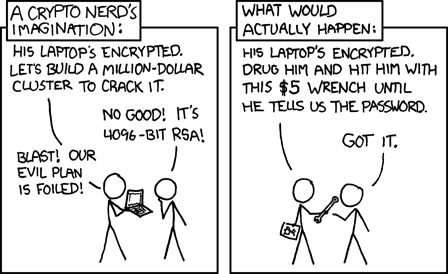
\includegraphics[width=0.75\textwidth]{figures/xkcd/xkcd_538_security.png}
    \caption[\texttt{xkcd} Security]{Here we have an example of cryptography
        in the wild.
        To defend against rubber-hose cryptanalysis,
        see~\cite{bojinov2012neuroscience}.
        Created by Randall Munroe on \texttt{xkcd};
        posted online at \url{https://xkcd.com/538/}.
        }
    \label{fig:xkcd_security}
\end{figure}


These notes may also be helpful to understand the cryptography in the
AliceNet Whitepaper~\cite{AliceNetWhitepaper}.
\emph{Full disclosure:} the author of the present work
helped write~\cite{AliceNetWhitepaper}.



\section{Intended Audience}

This document is written for individuals without a significant
background in mathematics.
The necessary mathematics for \gls{publiccrypto} involves
\gls{number theory} and algebra (\gls{group} theory, \gls{field} theory, and
\glspl{elliptic curve}).
The main requirement for learning this material is dedication.

Although this is primarily aimed at software engineers
interested in cryptography,
other technically-inclined individuals may find these notes helpful;
that is, the material presented here is meant to be accessible
to those who studied mathematics,
science, or engineering at the collegiate level.
Individuals who do not meet this criterion are still encouraged
to continue reading if the material is deemed sufficiently interesting.



\section{Examples}

Concrete examples will be used throughout to assist comprehension.
\texttt{Python} scripts are included that may easily be modified;
see \texttt{examples/} and its subdirectories.

We note that \texttt{code/} stores code for printed examples
throughout the text and is not meant to be modified;
this is separate from \texttt{examples/}, which is designed to be modified.


\section{Overview}

In Chapter~\ref{chap:do_not}, we focus on ``what not to do''.
This includes many bad ideas.
The main takeaway is this:
\textbf{do not write your own cryptographic algorithms or protocols}.

We start by introducing the mathematics used
throughout these notes in Chapters~\ref{chap:math_1},
\ref{chap:math_2}, and \ref{chap:math_3};
the material becomes progressively more abstract.
In Chapter~\ref{chap:math_3}, we discuss \glspl{elliptic curve},
\glspl{bilinear}, and \gls{lagrange interpolation};
this may be a bit advanced,
so on the initial reading this chapter may be skipped
and read at a future point in time.

After the mathematical review, we spend some time discussing
\gls{symmetriccrypto} in Chapter~\ref{chap:symmetric}.
This material is probably more familiar:
Alice and Bob share a secret key and want to communicate.
We spend significant time talking about \glspl{hash function};
\glspl{hash function} are first discussed in
Chapter~\ref{chap:hash} while their applications are discussed in
Chapter~\ref{chap:hash_applications}.

At this point, we focus on \gls{publiccrypto}
in Chapter~\ref{chap:public}.
In this case, Alice and Bob use 2 keys to communicate:
one public key and one private key.
We spend Chapter~\ref{chap:signatures} discussing an important
aspect of \gls{publiccrypto}: \glspl{signature}.
After this, we look at \gls{ecc} in Chapter~\ref{chap:elliptic};
this involves reworking material from Chapters~\ref{chap:public}
and \ref{chap:signatures} in terms of \glspl{elliptic curve}.

Starting with Chapter~\ref{chap:pairing} on \gls{pairingcrypto},
the material becomes more advanced.
After this, we discuss \glspl{zkproof} in Chapter~\ref{chap:zkproofs}.
To wrap up, we end with a discussion of secret sharing protocols
and \gls{distributed key generation} in Chapter~\ref{chap:secret_sharing};
the discussion here draws on material from essentially \emph{all}
of the previous chapters.

In Chapter~\ref{chap:hardness}, we discuss some of the hardness assumptions
in \gls{publiccrypto}.
If certain mathematical problems are hard to solve,
then the cryptographic protocols discussed here are secure.



\section{Cryptographic Participants}

We will frequently encounter Alice and Bob.
Alice and Bob will try to communicate without Eve
(an adversarial eavesdropper) determining what is being sent.
Other characters such as Charlie and Dave may pop up occasionally as well.
More characters may be found online%
\footnote{\url{https://en.wikipedia.org/wiki/Alice_and_Bob}}.



\section{Mathematical Precision}

In general, the author will try to be precise.
With that said, this is meant to be an \emph{introduction} to cryptography,
so definitions will not always be as precise as possible.
Care will be taken to refrain from using ``impossible''
unless it actually is.
For instance, if a \gls{otp} is used and the secret key is
uniformly random, then it is \emph{impossible} to decrypt the message
without the secret key.
This is \gls{perfect security}: no amount of computational power will enable
the \gls{otp} to be broken.
We will generally use ``impractical'' to describe situations
where a significant amount of computational effort is required;
for instance, breaking a system may require performing $2^{128}$
operations, which is thought to be impractical.

In most cases, only the material \emph{required} is mentioned
along with some related discussion.
At times, additional material is included in the appendices:
additional cryptography may be found in Appendix~\ref{app:crypto}
while additional mathematics may be found in Appendix~\ref{app:math}.
This material was deemed interesting or useful enough
to be included for the curious reader even if it is not
\emph{strictly necessary}.



\section{Additional Resources}

All of the material here may easily be gathered from other books and sources.
The author used many books to learn cryptography himself.
Specific paths for additional learning are discussed
in Chapter~\ref{chap:conclusion}.

\chapter{What Not to Do}
\label{chap:do_not}

This chapter is devoted to listing a bunch of \emph{horrible}
things to do;
we list them here precisely because you should \emph{never}
do any of these things.

\section{General Advice}

\begin{itemize}
\item \textbf{Do not ``roll your own crypto.''}
    It is always a good idea to use software that professional cryptographers
        have written.
    It is a bad idea to write your own \gls{encryption scheme},
        \gls{signature} scheme,
        \gls{hash function}, \dots
    Use something written by experts.
    That library should have been written by someone with many years
        of experience in cryptography and it should have been vetted
        by other people as well.

    Along those lines is a
    \href{https://www.schneier.com/crypto-gram/archives/1998/1015.html#cipherdesign}{quote}
    from Bruce Schneier in 1998:

\begin{quote}
    Anyone, from the most clueless amateur to the best cryptographer,
    can create an algorithm that he himself can't break.
    It's not even hard. What is hard is creating an algorithm
    that no one else can break, even after years of analysis.
\end{quote}

\item \textbf{Do not randomly combine cryptographic primitives
    to arrive at something you think solves the problem.}
    Take the time to think about \emph{exactly} what you are trying to do.
    If you are wanting to store passwords,
    then use a using a \gls{kdf} designed
    for password storage
    and not a standard \glsfirst{hash function};
    both are useful but serve different purposes.

\item \textbf{Whenever possible, do not use randomized algorithms.}
    There are many problems which may arise when using
        random number generators.
    Thus, whenever possible, use deterministic algorithms.
    There may be times when algorithms requiring randomness
    can be reworked to use ``deterministic randomness'' based on
    \glsfirstplural{hash function}.
    This would be the preferred method; see~\cite{rfc6979}.

\item \textbf{Do not use classical algorithms.}
    If any real security is required, do not \emph{ever} use
    classical algorithms like substitution or transposition ciphers.
    All classical ciphers can easily be brute-forced and may
    be broken given enough ciphertext.

\item \textbf{The only \gls{encryption scheme} with \gls{perfect security}
    is the \gls{otp}.}
    Any perfectly secure encryption scheme is equivalent to the
    \gls{otp}~\cite[Theorems 2.10 and 2.11]{IntroModernCrypto}.
    Anyone who claims to have a perfectly secure algorithm
    that is better than the \gls{otp} is \emph{lying}.

\item \textbf{Do not use ``security through obscurity'' or
    assume a secret algorithm will be sufficient for security.}
    This goes against
    \emph{Kerchoff's principle}~\cite[Page 5]{IntroModernCrypto}:

\begin{quote}
    The cipher method must not be required to be secret,
    and it must be able to fall into the hands of the enemy
    without inconvenience.
\end{quote}

\end{itemize}

\section{Symmetric Key Encryption}

\begin{itemize}
\item \textbf{Do not use ECB-mode when encrypting with a \gls{block cipher}.}
    ECB stands for \emph{Electronic Codebook}.
    This method should \emph{never} be used when performing
        encryption with a \gls{block cipher}.
    It leaks too much information.
\item \textbf{Do not use DES.}
    DES stands for \emph{Data Encryption Standard} and is a \gls{block cipher}.
    The small key size allows it to be easily broken~\cite{rfc4772}.
    The \emph{only} reason to ever use it is because its use is required
        for compatibility with legacy systems.
\item \textbf{Do not use RC4.}
    RC4 is a cryptographically-broken \gls{stream cipher}~\cite{rfc7465}.
\item \textbf{Do not use Blowfish.}
    Blowfish is an old \gls{block cipher},
    and in 2007 its author
    \href{https://www.schneier.com/news/archives/2007/12/bruce_almighty_schne.html}{recommended}
    switching from Blowfish to a different \gls{encryption scheme}.

\end{itemize}

\section{Cryptographic Hash Functions}

\begin{itemize}
\item \textbf{Do not use \MDFive{}.}
    \MDFive{} is a cryptographically-broken \gls{hash function}~\cite{rfc6151}.
    The \emph{only} reason to ever use it is because its use is required
        for compatibility with legacy systems.
\item \textbf{Do not use \ShaOne{}.}
    See the reasons above about why \MDFive{} should not be used~\cite{rfc6194}.
\item \textbf{Do not use PBKDF2 as a \gls{kdf}.}
    It has been shown to provide insufficient protection
    when protecting passwords~\cite{blocki2018economics}.
\item \textbf{Do not use \texttt{bcrypt} as a \gls{kdf}.}
    It has also been shown to provide insufficient protection
    when protecting passwords~\cite{blocki2018economics}.
\end{itemize}

\section{Cryptographically-Secure Pseudorandom Number Generators}

\begin{itemize}
\item \textbf{Do not use Dual\_EC\_DRBG.}
    The standard algorithm has the potential for a
    backdoor~\cite{BernsteinDualEC}.
\item \textbf{Do not use non-cryptographic PRNGs for cryptographic protocols.}
    Cryptographic protocols \emph{require} cryptographically-strong
    pseudorandom numbers;
    these numbers come from a \gls{csprng}.
    The numbers provided by non-cryptographic PRNGs
    \emph{are not sufficiently random}~\cite{marsaglia1968random,bouillaguet2020practical}.

    Here is a non-exhaustive list of non-cryptographic PRNGs:
    Linear Congruential Generator (LCG), Permuted Congruential Generator (PCG),
    Mersenne Twister.
    \emph{None} of these PRNGs should \emph{ever be used}
    in cryptographic situations.
\end{itemize}

\section{Public Key Encryption}

\begin{itemize}
\item \textbf{Do not use publish the private key.}
    This should go without saying.
\end{itemize}

\section{Digital Signatures}

\begin{itemize}
\item \textbf{Do not use publish the signing key.}
    This should go without saying.
\end{itemize}


\chapter{Mathematical Review: Set Theory, Number Theory, and Complexity}
\chaptermark{Mathematical Review 1}
\label{chap:math_1}

In this chapter we begin our mathematical review.
Depending on one's background, it may be useful to skip these
chapters and return to them as needed.

While the information here and in the following chapters will continually
get more abstract, we make an effort to include numerous
\emph{concrete examples}.
Furthermore, we will attempt to point out \emph{why} we need
the various mathematical objects as they arise.

\section{Mathematical Notation, Set Theory, and Functions}

We begin by reviewing standard mathematical notation,
the basics of set theory, and \glspl{function}.

\subsection{Introduction to Set Theory}

We use ``$\mathDef{}$'' when making definitions.
Thus,

\begin{equation}
    a \mathDef{} b
\end{equation}

\noindent
means that we \emph{define} $a$ as $b$ and may be read as
``$a$ is (defined to be) $b$''.

For our purposes, a \emph{\gls{set}} is a collection of elements or objects.
We suppose that $A$ is a \gls{set}.
If $a$ is an element of $A$, we write $a\in A$;
this may be read as ``$a$ is an element of $A$'' or ``$a$ is in $A$''.
If $a$ is not an element of $A$, we write $a\notin A$;
this may be read as ``$a$ is not an element of $A$'' or ``$a$ is not in $A$''.
We will always have that $a\in A$ or $a\notin A$
for all sets $A$ and elements $a$.
The \gls{set} which contains no elements $\braces{}$
is called the \emph{empty set}
and is denoted by $\emptyset$.

If the sets $A$ and $B$ contain the same elements,
then they denote the same set and we write $A = B$;
this may be read as ``$A$ equals $B$''.
Otherwise, $A$ and $B$ do not contain the same elements,
and we write $A\ne B$;
this may be read as ``$A$ does not equal $B$''.

If $B$ is a set and for every $b\in B$ we have $b\in A$, then $B$ is a subset
of $A$ and we write $B\subseteq A$.
We may read $B\subseteq A$ as ``$B$ is a subset of $A$''.
If $B$ is a subset of $A$ and $B$ is not equal to $A$,
then $B$ is a proper subset of $A$;
in this case, $B\subseteq A$ and there is some $a\in A$ such that $a\notin B$.
We may write this as $B\subset A$;
this may be read as ``$B$ is a proper subset of $A$''.
Given any set $A$, we always have that the empty set is a subset of $A$:
$\emptyset\subseteq A$.

Starting with one \gls{set}, we would like to make other \glspl{set}.
Let $X$ be a set and $P$ is some property that
elements of $X$ may or may not have.
If we want to define a new set $A$ as the set of all elements
in $X$ which have property $P$, we would write

\begin{equation}
    A \mathDef{} \braces{x\in X\mid P}.
\end{equation}

\noindent
This is ``set builder'' notation.
We should read $A \mathDef{} \braces{x\in X\mid P}$ as
``$A$ is (defined to be) the set of all $x$ in $X$ such that
(property) $P$ is true''.
Here, we use ``$\mid$'' as a separator that should be read as ``such that.''
When using set builder notation, the overall set $X$ may not always
be explicitly stated.

Within set builder notation, we may use ``$\exists$'' as shorthand
for ``there exists'' or ``there is'';
we may also use ``$\forall$'' as shorthand for ``for all''.
Outside of set builder notation, we will try to not use this shorthand.

We will be interested in operations between sets,
and we will want to combine them in various ways.
Let $A$ and $B$ be sets.
We have the following definitions:

\begin{align}
    A \cup B &\mathDef{} \braces{x \mid x\in A \text{ or } x\in B}
        \nonumber\\
    A \cap B &\mathDef{} \braces{x \mid x\in A \text{ and } x\in B}
        \nonumber\\
    A \setminus B &\mathDef{} \braces{a\in A \mid a\notin B}.
    \label{eq:math_set_theory_basic_set_ops}
\end{align}

\noindent
Thus, $A\cup B$ contains elements that are in $A$ or $B$;
this should be read ``$A$ union $B$''.
$A\cap B$ is the set containing elements that are in both $A$ and $B$;
this should be read ``$A$ intersect $B$''.
$A\setminus B$ is the set containing elements in $A$ that are not in $B$;
this could be read ``$A$ set minus $B$'' or ``$A$ minus $B$''.
See Figure~\ref{fig:math_set_venn} for a graphical representation
of these set operations.

\begin{figure}[t]
\centering
    \begin{subfigure}[t]{0.45\textwidth}
    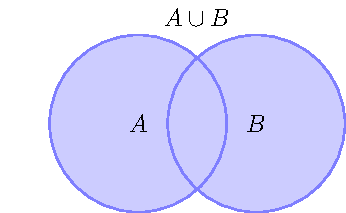
\includegraphics[width=\textwidth]{figures/math/set_theory/set_venn_or.pdf}
    \end{subfigure}
    \begin{subfigure}[t]{0.45\textwidth}
    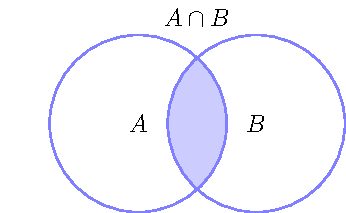
\includegraphics[width=\textwidth]{figures/math/set_theory/set_venn_and.pdf}
    \end{subfigure}

    \begin{subfigure}[t]{0.45\textwidth}
    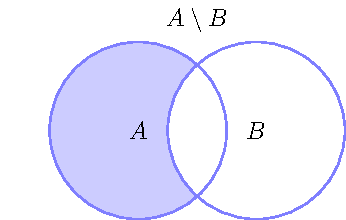
\includegraphics[width=\textwidth]{figures/math/set_theory/set_venn_minus.pdf}
    \end{subfigure}

    \caption[Set operations]{Here is a figure of various set operations:
        set union, set intersection, and set minus.
        Modified from the example
        \href{https://texample.net/tikz/examples/set-operations-illustrated-with-venn-diagrams/}{here}.}
    \label{fig:math_set_venn}
\end{figure}


\begin{example}[Examples of Sets and Set Operations]
We have the following definitions:

\begin{align}
    A &\mathDef{} \braces{0, 1, 2, 3}
        \nonumber\\
    B &\mathDef{} \braces{1, 2, 3, 4}
        \nonumber\\
    C &\mathDef{} \braces{1, 2, 3}
        \nonumber\\
    D &\mathDef{} \braces{1, 3, 5, 7}.
\end{align}

\noindent
Then we see

\begin{align}
    A \cup B &= \braces{0, 1, 2, 3, 4} \nonumber\\
    A \cap B &= \braces{1, 2, 3} \nonumber\\
        &= C \nonumber\\
    A \setminus B &= \braces{0}.
\end{align}

\noindent
We also note that all of the elements in $C$ are also in $A$ and $B$;
this implies that

\begin{align}
    C &\subseteq A
        \nonumber\\
    C &\subseteq B.
\end{align}

\noindent
Because $C\ne A$ and $C\ne B$, we have

\begin{align}
    C &\subset A
        \nonumber\\
    C &\subset B.
\end{align}

\noindent
Finally, we have

\begin{align}
    (A \cup C) \cup D &= \braces{0, 1, 2, 3, 5, 7} \nonumber\\
    (A \cap C) \cap D &= \braces{1, 3} \nonumber\\
    C \setminus D &= \braces{2} \nonumber\\
    C \setminus B &= \emptyset.
\end{align}
\end{example}

A further discussion of set theory may be found in
Appendix~\ref{app:math_set_theory}.

\subsection{Standard Mathematical Sets}
\label{ssec:standard_math_sets}

We have the following standard definitions for common collections
of numbers:

\begin{align}
    \N &\mathDef{} \braces{0, 1, 2, \ldots} \nonumber\\
    \Z &\mathDef{} \braces{\ldots, -2, -1, 0, 1, 2, \ldots} \nonumber\\
    \Q &\mathDef{} \braces{a/b \mid a,b\in\Z, b\ne0} \nonumber\\
    \R &\mathDef{} \braces{\text{the set of all real numbers}} \nonumber\\
    \C &\mathDef{} \braces{a + bi \mid a,b\in\R}.
\end{align}

\noindent
Naturally, we have the naturals $\N$, the integers $\Z$,
the rational numbers $\Q$, the real numbers $\R$,
and the complex numbers $\C$.

We also have the following standard definitions.
Not all of these will make sense at this time because
not everything has been defined.
We will discuss them in more detail in later chapters.

\begin{align}
    n\Z &\mathDef{} \braces{\ldots, -2n, -n, 0, n, 2n, \ldots}, \quad n\ge1
        \nonumber\\
    \Z_{n} &\mathDef{} \braces{0, 1, 2, \ldots, n-1}, \quad n>1\nonumber\\
    \Z_{n}^{*} &\mathDef{} \braces{a\in\Z_{n}\mid \gcd(a,n)=1}
        \nonumber\\
    \F_{p} &\mathDef{} \braces{0, 1, 2, \cdots, p-1}, \quad \text{$p$ prime}
        \nonumber\\
    \F_{p}^{*} &\mathDef{} \F_{p}\setminus\braces{0} \nonumber\\
    \braces{0,1}^{n} &\mathDef{} \braces{\text{The set of all $n$-bit strings}}
        \nonumber\\
    \braces{0,1}^{*} &\mathDef{}
        \braces{\text{The set of all finite bit strings}}.
\end{align}

\begin{example}[More Examples of Sets and Set Operations]
From the definitions, we see

\begin{align}
    \Z \cup \N &= \Z \nonumber\\
    \Z \cap \N &= \N \nonumber\\
    \Z \setminus \N &= \braces{\ldots, -3, -2, -1} \nonumber\\
    \Z \setminus \Q &= \emptyset.
\end{align}

\noindent
Additionally, for all sets $A$, we always have

\begin{align}
    A \cup \emptyset &= A \nonumber\\
    A \cap \emptyset &= \emptyset.
\end{align}
\end{example}

We write $a\chooseRandom{}A$ to denote that $a$ is chosen uniformly
at random from the \gls{set} $A$;
in this case, we assume that $A$ has a finite number of elements.

\subsection{Functions}

We will look at \glspl{function} between \glspl{set}.
Let $A$ and $B$ be \glspl{set}.
A \emph{\gls{function}} $f:A\to B$ uniquely assigns every element in
$a\in A$ to some element in $B$.
More specifically, for all $a\in A$ we have $f(a)\in B$.
We should read $f:A\to B$ as ``(a function) $f$ from $A$ to $B$''.
We say that $A$ is the \emph{domain} of $f$
and $B$ is the \emph{codomain} of $f$.
The \emph{range} of $f$ is defined to be $f(A)$:

\begin{equation}
    f(A) \mathDef{} \braces{b\in B \mid \exists a\in A, f(a) = b}.
    % TODO: possibly change to
    %       \braces{f(a)\in B \mid a\in A}.
\end{equation}

\noindent
This definition can be read as ``$f(A)$ is the set of all $b\in B$
such that there is an $a\in A$ so that $f(a) = b$''.
In this way, the range is everything that $f$ ``hits'':
if $\bar{b}\in f(A)$, then there is some $\bar{a}\in A$ with
$f(\bar{a}) = \bar{b}$.

\begin{example}[Example of a Function]
\label{example:function}
We let $A = \braces{0, 1, 2, 3}$ and $B = \braces{1, 2, 3, 4}$.
We define a \gls{function} $f:A\to B$ as follows:

\begin{align}
    f(0) &\mathDef{} 1 \nonumber\\
    f(1) &\mathDef{} 2 \nonumber\\
    f(2) &\mathDef{} 3 \nonumber\\
    f(3) &\mathDef{} 2.
\end{align}

\noindent
While we may sometimes think of \glspl{function} in terms of their graphs
like in Figure~\ref{fig:parabola_plot},
in this case we have fully specified $f$ by assigning every element in $A$
to some element in $B$;
thus, $f$ is a \gls{function}.

We see that

\begin{equation}
    f(A) = \braces{1,2,3} \subset B.
\end{equation}

\noindent
We have $1\in f(A)$ because $f(0) = 1$;
$2\in f(A)$ because $f(3) = 2$; and
$3\in f(A)$ because $f(2) = 3$.
Thus, the range $f(A)$ is a proper subset of the codomain $B$.
\end{example}

\begin{example}[Another Example of a Function]
We now have a more standard example of a \gls{function}.
We recall that $\R$ denotes the set of real numbers.

\begin{figure}[t]
\centering
    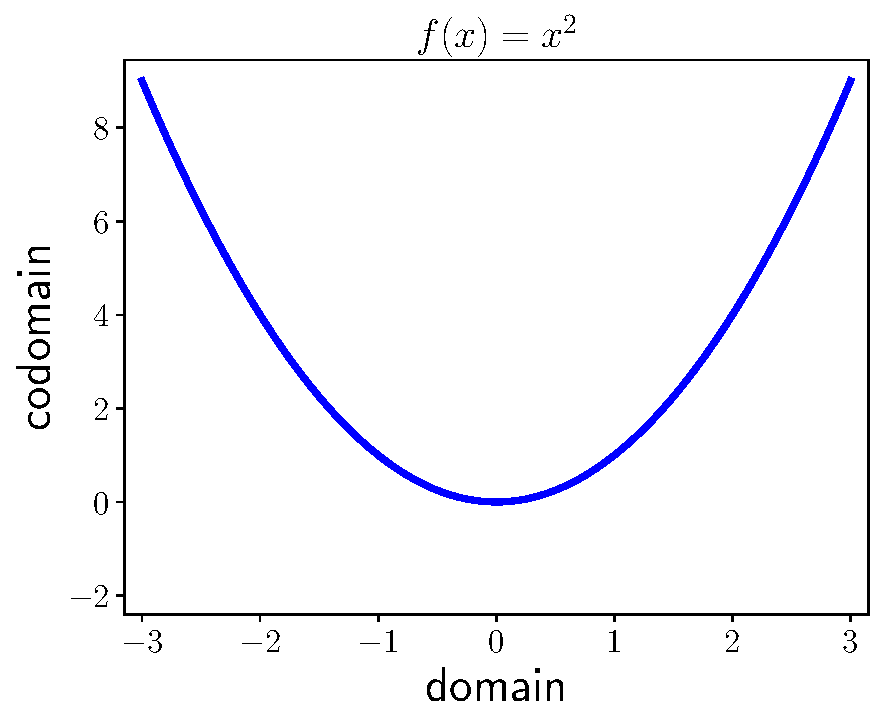
\includegraphics[width=10cm]{plots/parabola/function_parabola.pdf}
    \caption[Plot of a parabola]{Here
        we have a plot of the \gls{function} $f:\R\to\R$ with $f(x) = x^{2}$:
        the standard parabola.
        The domain of $f$ is the real numbers $\R$;
        the codomain of $f$ is also $\R$.
        We have that the range of $f$ is the \gls{set} of nonnegative
        real numbers: $f(\R) = [0,\infty)$.
        }
    \label{fig:parabola_plot}
\end{figure}


Let $f:\R\to\R$ and set $f(x) = x^{2}$.
In this case, the domain of the \gls{function} is $\R$
and the codomain of the \gls{function} is $\R$.
In this case, the range $f(\R) = [0,\infty)$.
We know the graph of $f$ is the standard parabola;
see Figure~\ref{fig:parabola_plot}.
\end{example}

\subsection{Function Properties}

We now list some standard properties that \glspl{function} may have:

\begin{itemize}
\item A \gls{function} $f:A\to B$ is \emph{\gls{injective}}
    or \emph{one-to-one} if $f(x) = f(y)$ implies that $x = y$.
    Equivalently, $f$ is injective if $x\ne y$ implies that $f(x) \ne f(y)$.
\item A \gls{function} $f:A\to B$ is \emph{\gls{surjective}} or \emph{onto}
    if for every $b\in B$ there is an $a\in A$ such that $f(a) = b$.
    This means that the range is equal to the codomain: $f(A) = B$.
\item A \gls{function} $f:A\to B$ is \emph{\gls{bijective}}
    (or $f$ is a \emph{bijection})
    if $f$ is both \gls{injective} and \gls{surjective}.
    In this case, $f$ has an \emph{inverse function} $g:B\to A$
    which satisfies

\begin{equation}
    g(f(a)) = a
\end{equation}

\noindent
and

\begin{equation}
    f(g(b)) = b
\end{equation}

\noindent
for all $a\in A$ and $b\in B$.
\end{itemize}

\begin{example}
The \gls{function} $f$ in Example~\ref{example:function}
is not \gls{injective}, \gls{surjective}, or \gls{bijective}.

\begin{itemize}
\item $f$ is not \gls{injective} because $f(1) = f(3) = 2$ but $1\ne3$.
\item $f$ is not \gls{surjective} because no element is mapped to $4\in B$.
\item $f$ is not \gls{bijective} because it is not
    \gls{injective} and \gls{surjective}.
\end{itemize}
\end{example}

\noindent
In preparation for more examples, we define the following functions:

\begin{align}
    f:\N\to\N,\quad &f(n) \mathDef{} n+1 \nonumber\\
    g:\Z\to\Z,\quad &g(n) \mathDef{} n+1 \nonumber\\
    h:\R\to\R,\quad &h(x) \mathDef{} x^{2}.
    \label{eq:math_set_theory_function_property_example_funcs}
\end{align}



\begin{example}[Injective Functions 1: Example]
\label{example:injective_functions_1}
We use the \gls{function} $f$ as defined in
Eq.~\eqref{eq:math_set_theory_function_property_example_funcs}.

If we have $n,m\in\N$ with

\begin{equation}
    f(n) = f(m),
\end{equation}

\noindent
this implies that

\begin{equation}
    n+1 = m+1,
\end{equation}

\noindent
so $n = m$.
Thus, $f$ is \gls{injective}.
\end{example}

\begin{example}[Injective Functions 2: Example]
\label{example:injective_functions_2}
We use the \gls{function} $g$ as defined in
Eq.~\eqref{eq:math_set_theory_function_property_example_funcs}.

Using the same argument from Example~\ref{example:injective_functions_1},
we see that $g$ is \gls{injective}.
\end{example}

\begin{example}[Injective Functions 3: Non-example]
\label{example:injective_functions_3}
We use the \gls{function} $h$ as defined in
Eq.~\eqref{eq:math_set_theory_function_property_example_funcs}.

For $x>0$, we see that $f(x) = f(-x)$ with $x\ne -x$.
In particular, we have $f(1) = f(-1) = 1$ but $1\ne-1$.
Thus, $h$ is not \gls{injective}.
\end{example}



\begin{example}[Surjective Functions 1: Non-example]
\label{example:surjective_functions_1}
We see that $f$ is not \gls{surjective},
because $0\in\N$ and there is no $n\in\N$ such that $f(n) = 0$.
\end{example}

\begin{example}[Surjective Functions 2: Example]
\label{example:surjective_functions_2}
Given $n\in\Z$, we see that $n-1\in\Z$ and

\begin{equation}
    g(n-1) = n.
\end{equation}

\noindent
Thus, $g$ is \gls{surjective}.
\end{example}

\begin{example}[Surjective Functions 3: Non-example]
\label{example:surjective_functions_3}
We see that $h$ is not \gls{surjective}.
This is because we know that for $x\in\R$, we have

\begin{equation}
    h(x) = x^{2}\ge0.
\end{equation}

\noindent
In particular, $-1\in\R$ yet there is no $x\in\R$ such that $h(x) = -1$.
\end{example}



\begin{example}[Bijective Functions 1: Non-example]
\label{example:bijective_functions_1}
In Example~\ref{example:injective_functions_1}
we showed that $f$ is \gls{injective}
while Example~\ref{example:surjective_functions_1}
showed that $f$ is not \gls{surjective};
thus, $f$ is not \gls{bijective}.
\end{example}

\begin{example}[Bijective Functions 2: Example]
\label{example:bijective_functions_2}
In Example~\ref{example:injective_functions_2}
we showed that $g$ is \gls{injective}
while Example~\ref{example:surjective_functions_2}
showed that $g$ is \gls{surjective};
thus, $g$ is \gls{bijective}.
\end{example}

\begin{example}[Bijective Functions 3: Non-example]
\label{example:bijective_functions_3}
In Example~\ref{example:injective_functions_3}
we showed that $h$ is not \gls{injective}
while Example~\ref{example:surjective_functions_3}
showed that $h$ is not \gls{surjective};
thus, $h$ is not \gls{bijective}.
\end{example}



\subsection{Permutations}

\Glspl{permutation} are a specific type of \gls{function};
in particular, \glspl{permutation} are bijections from a \gls{set} to itself.
More formally, if $A$ is a \gls{set},
the \gls{function} $f:A\to A$ is a \emph{\gls{permutation}}
if $f$ is \gls{bijective}.

\begin{example}[Permutations: Examples]
We let $A = \braces{1,2,3,4}$.

We define $f:A\to A$ by

\begin{align}
    f(1) &\mathDef{} 2
        \nonumber\\
    f(2) &\mathDef{} 3
        \nonumber\\
    f(3) &\mathDef{} 4
        \nonumber\\
    f(4) &\mathDef{} 1.
\end{align}

\noindent
Here, we see that $f$ is a \gls{permutation}.

Similarly, we can define $g:A\to A$ by

\begin{align}
    g(1) &\mathDef{} 4
        \nonumber\\
    g(2) &\mathDef{} 1
        \nonumber\\
    g(3) &\mathDef{} 2
        \nonumber\\
    g(4) &\mathDef{} 3.
\end{align}

\noindent
Here, $g$ is also a \gls{permutation}.
We can see that

\begin{align}
    f(g(1)) &= 1
        \nonumber\\
    f(g(2)) &= 2
        \nonumber\\
    f(g(3)) &= 3
        \nonumber\\
    f(g(4)) &= 4.
\end{align}

\noindent
Naturally, this formally shows that $f$ and $g$ are inverses.
\end{example}

\begin{example}[Permutations: Non-example]
As before, we let $A = \braces{1,2,3,4}$.

We define $h:A\to A$ by

\begin{align}
    h(1) &\mathDef{} 2
        \nonumber\\
    h(2) &\mathDef{} 3
        \nonumber\\
    h(3) &\mathDef{} 4
        \nonumber\\
    h(4) &\mathDef{} 4.
\end{align}

\noindent
We see that $h$ is not a \gls{permutation} because it is not a bijection.
In particular, $h$ is not \gls{injective} because $3,4\in A$
with $h(3) = h(4)$ yet $3\ne4$.
\end{example}

\section{Bit Operations}

Here we include a brief discussion of bit operations
for the sake of completeness.

\subsection{Definitions}

Each bit is either $\texttt{0}$ or $\texttt{1}$.

\paragraph{NOT}
\emph{NOT} reverses a bit:

\begin{align}
    \lnot\texttt{0} &= \texttt{1} \nonumber\\
    \lnot\texttt{1} &= \texttt{0}.
\end{align}

\paragraph{AND}
\emph{AND} operates on two bits and returns $\texttt{1}$ if both bits are
$\texttt{1}$ and returns $\texttt{0}$ otherwise:

\begin{align}
    \texttt{0}\land\texttt{0} &= \texttt{0} \nonumber\\
    \texttt{1}\land\texttt{0} &= \texttt{0} \nonumber\\
    \texttt{0}\land\texttt{1} &= \texttt{0} \nonumber\\
    \texttt{1}\land\texttt{1} &= \texttt{1}.
\end{align}

\paragraph{OR}
\emph{OR} operates on two bits and returns $\texttt{1}$ if at least one bit
is $\texttt{1}$ and returns $\texttt{0}$ otherwise:

\begin{align}
    \texttt{0}\lor\texttt{0} &= \texttt{0} \nonumber\\
    \texttt{1}\lor\texttt{0} &= \texttt{1} \nonumber\\
    \texttt{0}\lor\texttt{1} &= \texttt{1} \nonumber\\
    \texttt{1}\lor\texttt{1} &= \texttt{1}.
\end{align}

\paragraph{XOR}
\emph{XOR} operates on two bits and returns $\texttt{1}$
if the two bits are different and returns $\texttt{0}$ otherwise:

\begin{align}
    \texttt{0}\oplus\texttt{0} &= \texttt{0} \nonumber\\
    \texttt{1}\oplus\texttt{0} &= \texttt{1} \nonumber\\
    \texttt{0}\oplus\texttt{1} &= \texttt{1} \nonumber\\
    \texttt{1}\oplus\texttt{1} &= \texttt{0}.
\end{align}

\noindent
The XOR operation is important because of the following property:

\begin{equation}
    \parens{\texttt{x} \oplus \texttt{y}} \oplus \texttt{y} = \texttt{x}.
\end{equation}

\noindent
for all bits $\texttt{x}$ and $\texttt{y}$.
We also have

\begin{equation}
    \texttt{x} \oplus \texttt{0} = \texttt{x}.
\end{equation}

\subsection{Bit Operations on Integers}

Using an unsigned integer's binary representation,
these bit operations can be extended to unsigned integers;
the extension is straightforward and we only give examples.


\begin{example}[Bitwise Operations]
We show some examples of bit operations using 8-bit unsigned integers:

\begin{itemize}
\item Bitwise NOT:

\begin{align}
    \lnot\texttt{11110010} &=
         \texttt{00001101} \nonumber\\
    \lnot\texttt{11010011} &=
         \texttt{00101100} \nonumber\\
    \lnot\texttt{00010110} &=
         \texttt{11101001} \nonumber\\
    \lnot\texttt{10111011} &=
         \texttt{01000100}.
\end{align}

\item Bitwise AND:

\begin{align}
    \texttt{11110010} \land
    \texttt{11010011} &=
    \texttt{11010010} \nonumber\\
    \texttt{00010110} \land
    \texttt{10111011} &=
    \texttt{00010010}.
\end{align}

\item Bitwise OR:

\begin{align}
    \texttt{11110010} \lor
    \texttt{11010011} &=
    \texttt{11110011} \nonumber\\
    \texttt{00010110} \lor
    \texttt{10111011} &=
    \texttt{10111111}.
\end{align}

\item Bitwise XOR:

\begin{align}
    \texttt{11110010} \oplus
    \texttt{11010011} &=
    \texttt{00100001} \nonumber\\
    \texttt{00010110} \oplus
    \texttt{10111011} &=
    \texttt{10101101}.
\end{align}

In general, we also have

\begin{equation}
    \parens{x \oplus y} \oplus y = x
\end{equation}

\noindent
and

\begin{equation}
    x \oplus 0 = x
\end{equation}

\noindent
for all unsigned integers $x$ and $y$.
\end{itemize}
\end{example}

\section{Size of Numbers}

In \gls{publiccrypto} (which we discuss in Chapter~\ref{chap:public}),
we will need numbers to be of various magnitudes so that certain
mathematical problems are deemed sufficiently difficult;
the particular sizes are discussed in Chapter~\ref{chap:hardness}
when we talk about computational hardness assumptions.
We frequently represent integers in binary expansion,
so we use that to describe their sizes here.

Given $a\in\N$, we say that $a$ is a $k$-bit number if
$2^{k-1} \le a < 2^{k}$;
that is, the largest set bit in $a$'s binary expansion
is in the $k$th position.

\begin{example}[Size of Numbers]
\exampleCodeReference{examples/math\_review/size\_of\_numbers.py}

Here are some good order-of-magnitude estimates to keep in mind:

\begin{align}
    2^{32}   &\simeq 4\cdot10^{9}   \nonumber\\
    2^{64}   &\simeq 2\cdot10^{19}  \nonumber\\
    2^{128}  &\simeq 3\cdot10^{38}  \nonumber\\
    2^{256}  &\simeq 1\cdot10^{77}  \nonumber\\
    2^{512}  &\simeq 1\cdot10^{154} \nonumber\\
    2^{1024} &\simeq 2\cdot10^{308}.
\end{align}

\noindent
For reference, we note that the total number of particles
in the known universe is estimated to be $10^{80}$.
Additionally, a standard year has $31536000 \simeq 2^{25}$ seconds in it.
\end{example}

When working with cryptography in practice,
we may seek a certain level of security.
For instance, we may want ``128-bit security''.
This means that we want the most efficient algorithm for breaking
the underlying cryptosystem to require \emph{at least} $2^{128}$ operations.
As we can see, this is a large number.
Analogously, having $k$-bit security amounts to requiring
the most efficient algorithm must perform at least $2^{k}$ operations.

\begin{example}[How large is $2^{128}$?]
Let us suppose that we have $P$ processors
performing $F$ operations per second and run those processors for $S$ seconds.
The total number of operations $T$ that will be performed
in that amount of time will be

\begin{equation}
    T = P\cdot F\cdot S \quad\text{operations.}
\end{equation}

We now put in some concrete numbers.
Assume $P = 2^{30}$ processors (approximately one billion)
performing $F = 2^{30}$ operations per second (1 GHz)
for one year $S = 2^{25}$.
Then we have

\begin{align}
    T &= 2^{30}\cdot 2^{30} \cdot 2^{25} \nonumber\\
        &= 2^{85} \quad\text{operations.}
\end{align}

\noindent
At this rate, to perform $2^{128}$ operations would require
$2^{128-85} = 2^{43} \simeq 9\cdot10^{12}$ years.
It would take almost 10 trillion years at current capabilities
for perform $2^{128}$ operations.

While we should never try to estimate how computing will
advance in the future, it is clear that performing
$2^{128}$ operations is a daunting task.
Presumably, this is infeasible for at least the near future.
\end{example}

\subsection*{Converting between Powers of 2 and Powers of 10}

We have the following useful approximations:

\begin{align}
    10   &\simeq 2^{3} \nonumber\\
    100  &\simeq 2^{7} \nonumber\\
    1000 &\simeq 2^{10}.
\end{align}

\noindent
These approximations are slightly better:

\begin{align}
    10   &\simeq 2^{3.3} \nonumber\\
    100  &\simeq 2^{6.6} \nonumber\\
    1000 &\simeq 2^{10}.
\end{align}

\noindent
Even so, these approximations are probably not needed in practice,
especially if we just care about order-of-magnitude \emph{estimates}.

Based on $10^{3} = 1000 \simeq 1024 = 2^{10}$, we have the following:

\begin{align}
    2^{10} &\simeq 10^{3} \nonumber\\
    2^{20} &\simeq 10^{6} \nonumber\\
    2^{30} &\simeq 10^{9}.
\end{align}

\noindent
In general, we have

\begin{equation}
    2^{10k} \simeq 10^{3k}.
\end{equation}

\begin{example}[Power Conversions]
\exampleCodeReference{examples/math\_review/power\_conversion.py}

We will now work through some conversions.
We see

\begin{align}
    2^{86} &= 2^{6 + 10\cdot8} \nonumber\\
        &= 2^{6}\cdot2^{10\cdot8} \nonumber\\
        &\simeq 100\cdot10^{3\cdot8} \nonumber\\
        &= 10^{26}.
\end{align}

\noindent
A more exact approximation is

\begin{equation}
    2^{86} \simeq 7.7\cdot10^{25}.
\end{equation}

\noindent
Thus, $10^{26}$ is a good order-of-magnitude estimate.

Similarly,

\begin{align}
    10^{86} &= 10^{2 + 3\cdot28} \nonumber\\
        &= 100\cdot10^{3\cdot28} \nonumber\\
        &\simeq 2^{7}\cdot 2^{280} \nonumber\\
        &= 2^{287}.
\end{align}

\noindent
We see that

\begin{equation}
    \log_{2}(10^{86}) \simeq 285.7.
\end{equation}

\noindent
Thus, our approximation was not too far off:
we are within a factor of 4.

If instead we use the more accurate approximation $100 \simeq 2^{6.6}$,
then we have

\begin{equation}
    10^{86} \simeq 2^{286.6}.
\end{equation}

\noindent
This is within a factor of 2.
\end{example}

\section{Number Theory}

We review some basic facts of \gls{number theory} related to divisibility,
prime numbers, and modular arithmetic.
Additional material may be found in Appendix~\ref{app:math_nt}.
A more systematic treatment
may be found in~\cite{ComputationalIntroNTA}.

\subsection{Divisibility and Prime Numbers}

Given $a,b\in\Z$, we say $a$ divides $b$, written as $a\mid b$, when
$b = ca$ for $c\in\Z$;
in this case, we call $a$ a \emph{divisor} of $b$.
We write $a\nmid b$ when $a$ does not divide $b$ and say $a$ is not
a divisor of $b$.
Because $a = 1\cdot a$, we see that $1\mid a$ and $a\mid a$;
thus, $1$ and $a$ are always divisors of $a$.

If $p\in\N\setminus\braces{0,1}$ and we \emph{only} have
$1\mid p$ and $p\mid p$,
then we say that $p$ is a \emph{prime number}.
We frequently use $p$ and $q$ to denote prime numbers.
If $n\in\N\setminus\braces{0,1}$ and $n$ is not prime,
then we say that $n$ is \emph{composite}.

By convention, mathematicians do not consider $0$ or $1$
to be prime or composite numbers.

\begin{example}[Prime and Composite Numbers]
We know that $15 = 3\cdot 5$, so $15$ is a composite number.
We know that we only have $3 = 1\cdot 3$ and $5 = 1\cdot 5$,
so $3$ and $5$ are prime numbers.
\end{example}

\subsection{Greatest Common Divisor}

Given $a,b\in\Z$ (with $a\ne0$ or $b\ne0$), $d\ge0$ is the
\emph{greatest common divisor} of $a$ and $b$, written as
$\gcd(a,b) = d$, if $d$ is a divisor of $a$ and $b$ and that
if $r\ge0$ is also a divisor of $a$ and $b$ then $r\le d$.
When $\gcd(a,b) = 1$, we say that $a$ and $b$ are \emph{coprime}:
they have no common divisors.
Stated another way, coprime numbers have no common prime factors.

There are efficient algorithms to compute $\gcd(a,b)$;
see Appendix~\ref{app:math_nt} for more details.
One inefficient method involves computing the prime factorization
of $a$ and $b$ and then collecting the common factors.

\begin{example}[GCD Examples]
\label{example:bnt_gcd}
\exampleCodeReference{examples/math\_review/gcd.py}

We have $3 = 1\cdot3$ and $5 = 1\cdot5$;
this implies

\begin{equation}
    \gcd(3,5) = 1.
\end{equation}

\noindent
We know $15 = 3\cdot 5$;
this implies that

\begin{align}
    \gcd(15,5) &= 5 \nonumber\\
    \gcd(15,3) &= 3.
\end{align}

\noindent
We know $1872 = 2^{4}\cdot3^{2}\cdot13$ and
$1080 = 2^{3}\cdot3^{3}\cdot5$;
this implies that

\begin{align}
    \gcd(1872, 1080) &= 2^{3}\cdot3^{2} \nonumber\\
        &= 72.
\end{align}

\noindent
This is worked out in
Example~\ref{example:app_math_euclidean_alg}.
\end{example}

If $\gcd(a,b) = d$, then we can always find $x,y\in\Z$ such that

\begin{equation}
    ax + by = d.
\end{equation}

\noindent
There are efficient algorithms to compute this;
see Appendix~\ref{app:math_nt} for more details.

\begin{example}
\label{example:bnt_extended_gcd}
\exampleCodeReference{examples/math\_review/gcd.py}

We continue the previous example for $\gcd(1872, 1080) = 72$.
We see

\begin{equation}
    1872 \cdot (-4) + 1080 \cdot 7 = 72.
\end{equation}

\noindent
This is worked out in
Example~\ref{example:app_math_extended_euclidean_alg}.
\end{example}

\subsection{Congruent Numbers}

Let $n>1$ be an integer.
Given $a,b\in\Z$, we say that $a$ is congruent to $b$ modulo $n$
if $n\mid a-b$;
that is, we have $a-b = kn$ for some $k\in\Z$.
We also write this as $a \equiv b \mod n$.

\begin{example}[Examples of Congruent Numbers Mod 2]
We let $n=2$.
In this case, we see that $1 \equiv 11\mod 2$ because

\begin{equation}
    1 - 11 = \parens{-5}\cdot2.
\end{equation}

\noindent
Similarly, $2 \equiv 10 \mod 2$:

\begin{equation}
    2 - 10 = \parens{-4}\cdot2.
\end{equation}

\noindent
Continuing on, we see that all even numbers are congruent modulo $2$
and all odd numbers are congruent modulo $2$.

We show this now.
Let $a = 2k$ and $b = 2\ell$.
Then

\begin{equation}
    a - b = 2\parens{k-\ell}.
\end{equation}

\noindent
Thus, $a\equiv b \mod 2$.
This gives us the result for even numbers.
If $c = 2m+1$ and $d = 2n + 1$, then we see

\begin{equation}
    c - d = 2\parens{m-n}.
\end{equation}

\noindent
Thus, $c\equiv d \mod 2$.
This gives us the result for odd numbers.

We just showed that all even numbers are congruent to $0$ modulo $2$
and all odd numbers are congruent to $1$ modulo $2$.
\end{example}



\subsection{Modular Arithmetic}

Let $n>1$ be an integer.
Given $a\in\Z$, we can always compute $q, r\in\Z$ such that

\begin{equation}
    a = qn + r,
\end{equation}

\noindent
where $q$ the \emph{quotient}
and $0\le r < n$ the \emph{remainder};
this is called \emph{Euclidean Division}
and is discussed in Appendix~\ref{app:math_nt}.
From our previous discussion, we see that

\begin{equation}
    a\equiv r\mod n.
\end{equation}

\noindent
Using this fact, we will show that addition and multiplication
are always well-defined in modular arithmetic.
From there, exponentiation and other operations follow.
The only operation which requires care is division,
which we will look at separately.

\paragraph{Addition} We let $a_{1}, a_{2}\in\Z$ with

\begin{align}
    a_{1} &= q_{1}n + r_{1} \nonumber\\
    a_{2} &= q_{2}n + r_{2},
\end{align}

\noindent
where $q_{i}\in\Z$ and $0\le r_{i} < n$.
Then we see

\begin{align}
    a_{1} + a_{2} &= \parens{q_{1} + q_{2}}n + \parens{r_{1}+r_{2}}
        \nonumber\\
    &= r_{1} + r_{2} \mod n.
\end{align}

\noindent
This shows that addition behaves as we would expect.

\paragraph{Multiplication} We let $a_{1}$ and $a_{2}$ be as before.
Then

\begin{align}
    a_{1}a_{2} &= \parens{q_{1}q_{2}n + r_{1}q_{2} + r_{2}q_{1}}n + r_{1}r_{2}
        \nonumber\\
    &= r_{1}r_{2} \mod n.
\end{align}

\noindent
This shows that multiplication behaves as we would expect.

\paragraph{Division} We need to be careful in order to define division.
Within the rational or real numbers, when we say that $x$
is the multiplicative inverse of $a$,
we mean that

\begin{equation}
    ax = 1.
\end{equation}

We look for something similar in modular arithmetic.
Thus, if $a\in\Z\setminus\braces{0}$, then we look for an $x\ne0$ such that

\begin{equation}
    ax \equiv 1 \mod n.
\end{equation}

\noindent
This implies that there is $k\in\Z$ such that

\begin{equation}
    ax - 1 = -nk,
\end{equation}

\noindent
or rather

\begin{equation}
    ax + nk = 1.
\end{equation}

The above equality implies that

\begin{equation}
    \gcd(a,n) = 1.
\end{equation}

\noindent
Thus, if $\gcd(a,n) = 1$, then $a$ has a multiplicative inverse
modulo $n$.

\begin{example}[Modular Arithmetic Example]
\exampleCodeReference{examples/math\_review/modular\_arithmetic.py}

We let $n = 256$.
We have

\begin{align}
    27 + 241 &\equiv 12 \mod 256 \nonumber\\
    27 \cdot 241 &\equiv 107 \mod 256.
\end{align}

\noindent
Because $\gcd(27,256) = 1$ and $\gcd(241,256) = 1$,
$27$ and $241$ have multiplicative inverses.
We find that

\begin{align}
    27 \cdot 19 &\equiv 1 \mod 256 \nonumber\\
    241 \cdot 17 &\equiv 1 \mod 256.
\end{align}
\end{example}

\section{Computational Complexity}

We review the basics of computational complexity in order
to talk about the computational cost of solving certain problems.
That is to say, we care about how long certain operations
take when we look at asymptotically large values.

\subsection{Big-O Notation}

We begin by reviewing big-O notation.
Let $f:\N\to\R$ and $g:\N\to\R$ with $f(n)\ge0$ and $g(n)\ge0$.
We write $f(n) = O(g(n))$ when there is some $C>0$
and $N\in\N$ such that

\begin{equation}
    f(n) \le Cg(n), \quad n\ge N.
\end{equation}

\noindent
That is, $f$ is asymptotically bounded above by $g$.

We write $f(n) = \Omega(g(n))$ when there is some $C>0$
and $N\in\N$ such that

\begin{equation}
    f(n) \ge Cg(n), \quad n\ge N.
\end{equation}

\noindent
That is, $f$ is asymptotically bounded below by $g$.

Finally, we write $f(n) = \Theta(g(n))$ when $f(n) = O(g(n))$ and
$f(n) = \Omega(g(n))$.
That is, $f$ is asymptotically bounded above and below by $g$.
In general, we are interested in \emph{tightly} bounding functions
asymptotically; lose bounds are not very valuable.

A further discussion of Big-O notation may be found
in~\cite[Chapter 3]{IntroToAlgs} or
\cite[Chapter 1.2.11.1]{TAOCP1}.

\begin{example}[Example of Big-O Notation]
We let $f(n) = n^{2} + 10n + 5$ and $g_{1}(n) = n^{3}$.
Then we see

\begin{equation}
    f(n) \le 20\cdot g_{1}(n), \quad n\ge1.
\end{equation}

\noindent
Thus, $f(n) = O(g_{1}(n))$.

We now let $g_{2}(n) = n^{2}$.
In this case, we have

\begin{equation}
    f(n) \le 16\cdot g_{2}(n), \quad n\ge1.
\end{equation}

\noindent
Thus, $f(n) = O(g_{2}(n))$.
We see that $g_{1}$ is a larger upper bound for $f$ while $g_{2}$ matches
the growth of $f$ more closely.

We now focus on making the statement ``$g_{2}$ matches the growth
of $f$ more closely'' more precise;
in particular, we will show that $g_{2}$ asymptotically bounds $f$
above and below.
We see that

\begin{equation}
    f(n) \ge g_{2}(n), \quad n\ge1.
\end{equation}

\noindent
Thus, $f(n) = \Omega(g_{2}(n))$.
Together, we have $f(n) = \Theta(g_{2}(n))$.
\end{example}

\begin{example}[Another Example of Big-O Notation]
We consider the function $f(n) = 100\brackets{\ln n}^{2}$.

We begin by comparing this function to $g_{1}(n) = n$.
Looking at $N = e^{10}\simeq 2.2\cdot10^{4}$, we have

\begin{equation}
    f(N) = 10^{4} < 2.2\cdot10^{4} \simeq g_{1}(N).
\end{equation}

\noindent
This holds for all $n\ge N$, so we have $f(n) = O(g_{1}(n))$.
Because $g_{1}$ grows much more quickly than $f$,
this bound is not very valuable.

We set $g_{2} = \brackets{\ln n}^{2}$.
Then we see that

\begin{equation}
    f(n) = 100\brackets{\ln n}^{2} \le 1000\brackets{\ln n}^{2}
\end{equation}

\noindent
and

\begin{equation}
    f(n) = 100\brackets{\ln n}^{2} \ge \brackets{\ln n}^{2}.
\end{equation}

\noindent
These inequalities hold for all $n$.
Thus, we have $f(n) = \Theta(g_{2}(n))$.
\end{example}

\subsection{Standard Complexity Classes}

We will now discuss some broad complexity classes.

Generally, we think of two classes: polynomial algorithms
and exponential algorithms.
Polynomial algorithms have time and space requirements bounded above
by a polynomial.
Exponential algorithms have time and space requirements
bounded above by an exponential function.

When working in computational (or algorithmic) number theory,
we seek algorithms which are polynomial in the \emph{bits} of $n$,
not polynomial in $n$.
Thus, we seek algorithms with total complexity cost

\begin{equation}
    C(n) = O\parens{\brackets{\log n}^{c}}
\end{equation}

\noindent
for some constant $c>0$.
This is called a \emph{polynomial algorithm};
its run time is bounded above by a polynomial in the bits of $n$.

If an algorithm has total complexity cost

\begin{equation}
    C(n) = O\parens{n^{c}}
\end{equation}

\noindent
for some constant $c>0$,
then the algorithm is \emph{exponential} in the bits of $n$.
This is called an \emph{exponential algorithm};
its run time is bounded above by a function exponential in the bits of $n$.
Because all polynomial algorithms are trivially exponential algorithms,
we generally assume the cost is bounded below by an exponential as well.
In the case of probabilistic algorithms,
the \emph{expected} run time is exponential.

It is possible to talk about superpolynomial algorithms
(algorithms which grow faster than any polynomial)
and subexponential algorithms
(algorithms which grow slower than any exponential)
but we will not discuss them at this point.
We do note that there are many open questions in computer science
related to the asymptotic complexity of various algorithms.
This is related to the computational complexity of
certain mathematical problems which we will discuss
in Chapter~\ref{chap:hardness}.

\subsection{Complexity of Various Operations}

There are polynomial algorithms for addition,
multiplication, exponentiation, greatest common divisor, and many others.
Currently, there are \emph{no known} polynomial algorithms
for integer factorization.
The fastest algorithms for factoring integers are subexponential algorithms.


\chapter{Mathematical Review: Groups, Rings, and Fields}
\chaptermark{Mathematical Review 2}
\label{chap:math_2}

We now build on our mathematical discussion from Chapter~\ref{chap:math_1}.
Here, we focus on the algebraic objects known as \glspl{group},
\glspl{ring}, and \glspl{field}.
These mathematical objects enable us to discuss the specifics
of \gls{publiccrypto}.

To assist in this discussion, we will first begin with intuition
and examples before giving the formal definition;
we include non-examples as well.

\section{Groups}
\label{sec:math_groups}

\subsection{Why do we care about Groups?}
\Glspl{group} arise in many different areas.
In cryptography, we will encounter them in the \gls{dhke}
and \glspl{signature}.
For \glspl{group} to be used in practice, we will need to encode them;
that is, we will need to know how to represent them on a computer.

\subsection{Intuition and Examples}
\emph{\Glspl{group}} are mathematical objects which we will
frequently encounter.
Informally, a \gls{group} is a generalization of the integers under addition,
so we start by looking at them first.

\begin{example}[Integers under addition]
The standard example of a \gls{group} is to consider the
integers $\Z$ under addition.

Given $a,b\in\Z$, we know that $a+b\in\Z$.
This means that the integers are \emph{closed} under addition:
adding two integers will always give us another integer.

Addition is also \emph{\gls{associative}}.
That is, for $a,b,c\in\Z$, we have

\begin{equation}
    \parens{a + b} + c = a + \parens{b + c}.
\end{equation}

\noindent
In this way, we do not have to worry about which way we add integers;
we will always get the same result regardless of order.

There is also a special integer $0\in\Z$.
It is special in that adding $0$ to $a$ gives us $a$:

\begin{equation}
    0 + a = a + 0 = a.
\end{equation}

\noindent
No other integer has this property.

We also know the (additive) inverse of $a$: $-a$.
This is because

\begin{equation}
    a + (-a) = 0.
\end{equation}

\noindent
It also turns out that the (additive) inverse is \emph{unique}.

We note that every integer can be written as
repeated additions of $1$.
If $a\ge0$, then we have

\begin{equation}
    a = \underbrace{1 + 1 + \cdots + 1}_{\text{$a$ times}} \quad a\ge 0.
    \label{eq:math_groups_integers_1_gen_pos}
\end{equation}

\noindent
For this to apply to negative numbers, we allow for adding $1$'s
additive inverse $-1$.
If $a<0$, then

\begin{equation}
    a = \underbrace{(-1) + (-1) + \cdots + (-1)}_{\text{$\abs{a}$ times}}
        \quad a < 0.
    \label{eq:math_groups_integers_1_gen_neg}
\end{equation}

\noindent
In this way, $1$ \emph{generates} the \gls{group} of integers under addition.

We also notice that addition is \emph{\gls{commutative}}:
given $a,b\in\Z$, we have

\begin{equation}
    a + b = b + a.
\end{equation}

\noindent
Although not all \glspl{group} have this property, the ones we care about do.
\end{example}

\begin{example}[Rationals under addition]
Similar to the integers under addition, the rational numbers $\Q$
under addition also form a \gls{group}.

Given $a,b\in\Q$ with $a = p/q$ and $b = r/s$,
we know

\begin{align}
    a + b &= \frac{p}{q} + \frac{r}{s} \nonumber\\
        &= \frac{ps + qr}{qs}\in\Q.
\end{align}

\noindent
This shows us that the rationals are closed under addition.

We know that addition of rationals is \gls{associative} and \gls{commutative}.
Furthermore, $0\in\Q$ is the identity element.
If $a = \frac{p}{q}$ as above, then the inverse is

\begin{equation}
    -a = \frac{-p}{q}
\end{equation}

\noindent
because

\begin{align}
    a + \parens{-a} &= \frac{p}{q} + \frac{-p}{q} \nonumber\\
        &= \frac{pq - pq}{q^{2}} \nonumber\\
        &= 0.
\end{align}

\noindent
This shows that the rationals under addition form a \gls{group}.
\end{example}

\begin{example}[Integers under modular addition]
We now look at another standard example: integers under modular arithmetic.
Let $n > 1$.
Then

\begin{equation}
    \Z_{n} = \braces{0, 1, \cdots, n-1}.
\end{equation}

\noindent
For $a,b\in\Z_{n}$, we know there is some $c\in\Z_{n}$ such that

\begin{equation}
    a + b = c \mod n.
\end{equation}

\noindent
This shows us that $\Z_{n}$ is closed under addition.

We know $0\in\Z_{n}$ and we always have

\begin{equation}
    0 + a = a + 0 = a
\end{equation}

\noindent
for $a\in\Z_{n}$.
Thus, $0$ is the additive identity.

Given $a\in\Z_{n}\setminus\braces{0}$, we know

\begin{equation}
    a + \parens{n-a} = 0 \mod n,
\end{equation}

\noindent
Thus, the additive inverse of $a$ is $n-a$;
$0$ is its own additive inverse.
Therefore, we see that $\parens{\Z_{n},+}$ is a \gls{group}.
\end{example}

\begin{example}[Positive Rationals under multiplication]
Similar to the integers under addition, the positive rational
numbers $\Q^{+}$ under multiplication form a \gls{group}.
In this case, the multiplicative identity is $1$.
\end{example}

\begin{example}[Nonexample: Natural numbers under addition]
We know that the natural numbers under addition are
very similar to the integers under addition.
We know that we can always add two natural numbers,
so that $a,b\in\N$ implies $a+b\in\N$;
thus, the naturals are closed under addition.
Addition is also \gls{associative} and \gls{commutative}.

We also have the identity $0\in\N$, so

\begin{equation}
    a + 0 = a
\end{equation}

\noindent
for all $a\in\N$.

Unfortunately, we do not have additive inverses;
this is because the natural numbers do not include the negative integers.
That is, for $a\in\N\setminus\braces{0}$, there is no $b\in\N$ such that

\begin{equation}
    a + b = 0.
\end{equation}

\noindent
Thus, $\parens{\N,+}$ is \emph{not} a \gls{group}.
\end{example}

\subsection{Formal Definition}

\begin{defn}[Group]
A \gls{group} is a \gls{set} $G$ together with a binary operation $\cdot$
such that, given $a,b\in G$, $a\cdot b\in G$;
that is, $G$ is closed under the binary operation $\cdot$.

The binary operation also satisfies the following properties:

\begin{itemize}
\item Associativity: for all $a,b,c\in G$, we have

\begin{equation}
    \parens{a\cdot b}\cdot c = a\cdot \parens{b\cdot c}.
\end{equation}

\item Identity element: there is an element $e\in G$ such that
    for all $a\in G$,

\begin{equation}
    a\cdot e = e\cdot a = a.
\end{equation}

\item Inverses: for every $a\in G$ there is a $b\in G$ such that
    
\begin{equation}
    a\cdot b = b\cdot a = e.
\end{equation}

\noindent
We henceforth denote the inverse of $a$ as $a^{-1}$.
\end{itemize}
\end{defn}

Formally, we write that $\parens{G,\cdot}$ is a \gls{group}.
Informally, we write that $G$ is a \gls{group} when the operation is understood.
Additionally, we frequently write $ab$ for $a\cdot b$.

\subsection{Continued Discussion}
Although the generic group operation was listed as ``multiplication'',
we could very well have used addition.
We will sometimes refer to some \glspl{group} as ``multiplicative groups''
while others as ``additive groups'';
this just means we use the multiplication sign $\cdot$
or the addition sign $+$ to denote the group operation.
Nothing changes, as we can use both symbols,
but there are conventions.
In additive groups, the identity element is usually denoted $0$;
in multiplicative groups, the identity element is usually denoted $1$.

Because $\parens{\Z,+}$ is a \gls{group}, we know that \glspl{group} can have
an infinite number of elements.
In what follows, we will be particularly interested
in \emph{\glspl{finite group}}:
\glspl{group} that have a finite number of elements.
We let $\abs{G}$ denote the order of the \gls{group}
(the number of elements in $G$).

At times, we may drop explicit reference to the operation if it is understood.
For instance, we may refer to $\Z$ as a \gls{group},
when more formally we should say $\parens{\Z,+}$ is a \gls{group}
in order to reference both the \emph{\gls{set}} (the integers $\Z$)
and the \emph{operation} (integer addition).
Even so, this is long, tedious, and painful, so we will,
at times, forego the formalities when the operation is clear
from the context.

\subsection{More Definitions}
Let $G$ be a \gls{group} and $H \subseteq G$;
more explicitly, $\parens{G,\cdot}$ is a \gls{group} and $H$ is a subset of $G$.
We say that $H$ is a \emph{\gls{subgroup}} of $G$, written as $H \le G$,
if $H$ with the group operation inherited from $G$ is also a \gls{group}.
Every \gls{group} $G$ has at least two \glspl{subgroup}:
$G$ (the entire group) and $\braces{e}$
(the group that is just the identity element $e$).
A \gls{subgroup} is called a \emph{proper subgroup} when
$H\le G$ and $H\ne G$.
If $H$ is a proper subgroup, then we may write $H < G$.
The \gls{group} $\braces{e}$ is called the \emph{trivial} subgroup.

\begin{example}[Subgroup Example: $2\Z \le \Z$]
We let

\begin{equation}
    2\Z \mathDef{} \braces{\ldots, -4, -2, 0, 2, 4, \ldots};
\end{equation}

\noindent
that is, $2\Z$ is the set of even integers.
Naturally, we have $2\Z\subseteq\Z$.
For every $a\in2\Z$ there is some $b\in\Z$ so that $a = 2b$.

Given $x,y\in2\Z$, we set $x = 2m$ and $y = 2n$ for $m,n\in\Z$.
We then see

\begin{align}
    x + y &= 2m + 2n \nonumber\\
        &= 2\parens{m+n}\in2\Z.
\end{align}

\noindent
Thus, $2\Z$ is closed under addition.
Because addition on $\Z$ is \gls{associative},
addition on $2\Z$ is also \gls{associative}.

Because $0\in\Z$ and

\begin{equation}
    0 + x = x\in2\Z,
\end{equation}

\noindent
we still have the same identity element $0\in2\Z$.

We let $x\in2\Z$ with $x = 2m$ for $m\in\Z$.
If $y = -2m$, then $y\in\Z$ and

\begin{align}
    x + y &= 2m + \parens{-2m} \nonumber\\
        &= 0\in2\Z.
\end{align}

\noindent
Thus, we see that every element in $2\Z$ has an additive inverse
within $2\Z$.
We have just shown that $\parens{2\Z,+}$ is a \gls{group};
because $2\Z\subseteq\Z$, $2\Z$ is a \gls{subgroup} of $\Z$.

In general, for $n\in\N\setminus\braces{0}$ we let

\begin{equation}
    n\Z \mathDef{} \braces{\ldots, -2n, -n, 0, n, 2n, \ldots}.
\end{equation}

\noindent
Then $n\Z\le\Z$.
This is a \emph{proper} subgroup when $n\ge2$.
\end{example}

For a multiplicative group $\parens{G,\cdot}$ and $g\in G$, we define

\begin{equation}
    \angles{g} \mathDef{} \braces{g^{n} \mid n\in\Z}.
\end{equation}

\noindent
In this case, we see that $\angles{g}$ contains all group elements
of the form $g^{n}$ for $n\in\Z$.
This is similar to Eqs.~\eqref{eq:math_groups_integers_1_gen_pos}
and \eqref{eq:math_groups_integers_1_gen_neg}.
Here, we have

\begin{equation}
    g^{n} = \underbrace{g \cdot g \cdots g}_{\text{$n$ times}} \quad n\ge 0
\end{equation}

\noindent
and

\begin{equation}
    g^{n} = \underbrace{g^{-1} \cdot g^{-1} \cdots g^{-1}}_{\text{$\abs{n}$
        times}} \quad n < 0.
\end{equation}

\noindent
In this case, $\angles{g}$ is the \gls{subgroup} of $G$ which consists
of products of $g$ or $g^{-1}$;
this allows us to write $\angles{g}\le G$.
We say $G$ is a \emph{\gls{cyclic group}} if there is a $g\in G$ such that
for all $h\in G$ there is an $n\in\Z$ such that $h = g^{n}$.
In this case, we have $G = \angles{g}$ and 
say that $g$ is a \emph{generator} of $G$.
\Glspl{cyclic group} are important in cryptography because
these \glspl{group} are used in the \gls{dhke};
they are also used to construct \glspl{signature}.

\begin{example}[Cyclic Group: $\Z$]
As we saw previously, $1$ is a generator of the integers $\Z$ under addition.
Thus, we can write $\angles{1} = \Z$.
We note that $-1$ is also a generator, so $\angles{-1} = \Z$.
\end{example}

\begin{example}[Non-cyclic Group: $\Q$]
We can consider the rational numbers $\Q$ under addition.
For any $a \in \Q\setminus\braces{0}$, we know that
and $\frac{a}{2}\in\Q\setminus\braces{0}$.
Even so, we see that $\frac{a}{2} \not\in \angles{a}$.
Thus, $\Q$ is not a \gls{cyclic group}.
\end{example}

In all of the groups we have looked up to this point,
all of our group operations satisfy $a\cdot b = b\cdot a$;
that is, the group operation is \emph{\gls{commutative}}.
We say that $G$ is an \emph{\gls{abelian group}} if for all $a,b\in G$
we have $a\cdot b = b\cdot a$.
This need not always be the case, but we will only consider
\glspl{abelian group} here because the \glspl{group} which normally arise
in cryptography are abelian.

We note that addition and multiplication are familiar
\gls{commutative} operations;
we always have $a+b = b+a$ and $a\cdot b = b\cdot a$ for real numbers.
We know that subtraction and division are \emph{not} \gls{commutative};
in general, we have $a-b \ne b-a$ and $\frac{a}{b} \ne \frac{b}{a}$.

We will usually denote $a\cdot b$ as $ab$ from now on
when there is no cause for confusion.

\subsection{Encoding Groups}

When working with the group $\Z_{n}$,
we can encode $k\in\Z_{n}$ by its binary representation.
Other groups may have different representations.

\section{Rings}
\label{sec:math_rings}

\subsection{Why do we care about Rings?}
\Glspl{ring} arise in many different areas.
We use \glspl{ring} to ease our way into the discussion about
\glspl{field} in Chapter~\ref{sec:math_fields}.

\subsection{Intuition and Examples}
\emph{\Glspl{ring}} are mathematical objects which we will sometimes encounter.
They are a generalization of the integers when we look
at both addition \emph{and} multiplication of integers.
We begin with some examples.

\begin{example}[Integers under addition and multiplication]
We know that we can add and multiply integers and remain
in the set of integers.
In this way, the integers are closed under addition
and closed under multiplication.
We also note that both addition and multiplication are \gls{associative}.
We know that both addition is \gls{commutative};
multiplication is also \gls{commutative},
but here we emphasize the \gls{commutative} nature of addition.

In the case of addition, we know that $0\in\Z$ is the additive inverse:
for every $a\in\Z$, we have

\begin{equation}
    0 + a = a + 0 = a.
\end{equation}

\noindent
Similarly, we have that $1\in\Z$ is the multiplicative inverse:
we have

\begin{equation}
    1\cdot a = a\cdot1 = a
\end{equation}

\noindent
for all $a\in\Z$.

We also know that addition and multiplication follow certain rules.
In particular, given $a,b,c\in\Z$, we have

\begin{equation}
    a\cdot\parens{b+c} = \parens{a\cdot b} + \parens{a\cdot c};
\end{equation}

\noindent
that is, we can \emph{distribute} multiplication over addition.
We also have

\begin{equation}
    \parens{a+b}\cdot c = \parens{a\cdot c} + \parens{b\cdot c}.
\end{equation}
\end{example}

\begin{example}[Integers modulo $n$]
We now look at modular arithmetic.
To be concrete, we look at $\Z_{6}$.
This satisfies all of the properties of the integers under addition
and multiplication.

One interesting property of $\Z_{6}$ but not $\Z$ is that $2,3\in\Z_{6}$
with $2\ne0$ and $3\ne0$ but

\begin{equation}
    2\cdot 3 = 0 \mod 6.
\end{equation}

\noindent
This is an example where two nonzero elements may be multiplied
together to equal zero.
Thus, we can see that there is something distinctly different
between $\Z$ and $\Z_{6}$.
\end{example}

\subsection{Formal Definition}

\begin{defn}[Ring]
A \gls{ring} is a \gls{set} $R$ together with two binary operations addition $+$
and multiplication $\cdot$.
First, $R$ is closed under addition and multiplication.
Furthermore, we have the following properties:

\begin{itemize}
\item $\parens{R,+}$ is an \gls{abelian group} with additive identity $0$.
    This implies that addition is \gls{associative}.
\item Multiplication is \gls{associative} on $R$; that is,
    for all $a,b,c \in R$, we have

\begin{equation}
    \parens{a\cdot b}\cdot c = a\cdot\parens{b\cdot c}.
\end{equation}
\item There is multiplicative identity $1\in R$; that is, 
    for all $a\in R$, we have

\begin{equation}
    1\cdot a = a\cdot 1 = a.
\end{equation}

\noindent
Furthermore, $0\ne 1$.

\item We have the following distribution laws between multiplication
    and addition.
    For all $a,b,c\in R$, we have

\begin{align}
    a\cdot\parens{b + c} &= \parens{a\cdot b} + \parens{a\cdot c}
        \nonumber\\
    \parens{b + c}\cdot a &= \parens{b\cdot a} + \parens{c\cdot a}
\end{align}
\end{itemize}

\noindent
We formally write $\parens{R,+,\cdot}$ is a ring.
\end{defn}

The above definition holds for all rings.
A \emph{\gls{commutative ring}} is one where multiplication
is \gls{commutative};
that is $a\cdot b = b\cdot a$ for all $a,b\in R$.
We will focus on \glspl{commutative ring} here because those will arise
in our work moving forward.
Thus, our distribution law reduces to 

\begin{equation}
    a\cdot\parens{b + c} = \parens{a\cdot b} + \parens{a\cdot c}.
\end{equation}

\subsection{Continued Discussion}

We say that  $a\in R\setminus\braces{0}$ is a \emph{zero divisor}
if there exists $b\in R\setminus\braces{0}$ such that $ab = 0$.

\begin{example}[Example of Zero Divisors]
We continue to look at the \gls{ring} $\Z_{6}$.
We have $2,3\in\Z_{6}$ with $2\ne0$ and $3\ne0$, yet we know

\begin{equation}
    2\cdot 3 = 6 \equiv 0 \mod 6.
\end{equation}

\noindent
This implies that $2$ and $3$ are zero divisors in $\Z_{6}$.

More generally, let $n = pq$ for distinct primes $p$ and $q$.
Then $p,q\in\Z_{n}$ and we know

\begin{equation}
    p\cdot q = n \equiv 0 \mod n.
\end{equation}

\noindent
This shows that $p$ and $q$ are zero divisors in $\Z_{n}$.
\end{example}

\begin{example}[Non-example of Zero Divisors]
While we may not have used this language before,
$\Z$ has no zero divisors.
We know (although we have not shown) that for $a,b\in\Z$ with
$ab = 0$ implies that $a=0$ or $b=0$.

This shows that the \gls{ring} $\parens{\Z,+,\cdot}$
is very different from the \glspl{ring} $\parens{\Z_{n},+,\cdot}$
when $n$ is composite.
\end{example}

\subsection{Encoding Rings}

When working with the \gls{ring} $\Z_{n}$, we can encode $k\in\Z_{n}$
by its binary representation.
Other rings have different representations.

\section{Fields}
\label{sec:math_fields}

\subsection{Why do we care about Fields?}
\Glspl{field} arise in many different areas.
In cryptography, we use \glspl{field} in \gls{dhke} and \glspl{signature}.
Additionally, \glspl{field} are used when working with \glspl{elliptic curve}.

\subsection{Intuition and Examples}
\emph{\Gls{field}} are common mathematical objects.
All \glspl{field} are \glspl{ring} but have additional properties.
Informally, a \gls{field} is a generalization of the rational numbers
with addition and multiplication.
In particular, every nonzero element has a multiplicative inverse.
We begin with some examples.

\begin{example}[The Rational Numbers]
The rational numbers are a standard example of a \gls{field}.
For $a\in\Q\setminus\braces{0}$, we can write

\begin{equation}
    a = \frac{m}{n}
\end{equation}

\noindent
for $m,n\in\Z\setminus\braces{0}$.
Then $\frac{n}{m}\in\Q$ and

\begin{equation}
    \frac{m}{n} \cdot \frac{n}{m} = 1.
\end{equation}

\noindent
Thus, $a$ has multiplicative inverse.
The rational numbers $\Q$ have an infinite number of elements.
\end{example}

\begin{example}[The Field $(\Z_{11},+,\cdot)$]
\exampleCodeReference{examples/math\_review/finite\_field\_inverses.py}

Let us look at $\Z_{11}$.
We have the following multiplication facts:

\begin{align}
    1\cdot 1 &= 1 \mod 11
        &
    6\cdot 2 &= 1 \mod 11 \nonumber\\
    2\cdot 6 &= 1 \mod 11
        &
    7\cdot 8 &= 1 \mod 11 \nonumber\\
    3\cdot 4 &= 1 \mod 11
        &
    8\cdot 7 &= 1 \mod 11 \nonumber\\
    4\cdot 3 &= 1 \mod 11
        &
    9\cdot 5 &= 1 \mod 11 \nonumber\\
    5\cdot 9 &= 1 \mod 11
        &
    10\cdot 10 &= 1 \mod 11.
\end{align}

\noindent
This shows that every nonzero element in $\Z_{11}$ has a multiplicative
inverse.
This, along with the other \gls{ring} properties, makes $\Z_{11}$ a \gls{field}.
In this case, we write it as $\F_{11}$ to emphasize the \gls{field} nature.
The \gls{field} $\F_{11}$ has a finite number of elements.
\end{example}

\subsection{Formal Definition}
\begin{defn}[Field]
A \gls{field} is a \gls{set} $F$ together with two binary operations
addition $+$ and multiplication $\cdot$ which have the following properties:

\begin{itemize}
\item $\parens{F,+}$ is an \gls{abelian group} with additive identity $0$.

\item $\parens{F^{*},\cdot}$ is an \gls{abelian group} with multiplicative
    identity $1$.
    Here, $F^{*} \mathDef{} F\setminus\braces{0}$.

\item We have $0\ne 1$.

\item We have the following distribution law between multiplication
    and addition.
    For all $a,b,c\in F$, we have

\begin{equation}
    a\cdot\parens{b + c} = \parens{a\cdot b} + \parens{a\cdot c}.
\end{equation}
\end{itemize}

\noindent
We formally say that $\parens{F,+,\cdot}$ is a \gls{field}.
\end{defn}

\subsection{Continued Discussion}

\subsubsection{Difference Between Rings and Fields}

We note that a \gls{field} is a \gls{commutative ring} with no zero divisors
and where every nonzero element has a multiplicative inverse.

\subsubsection{Finite Fields}

While the \glspl{field} of the rationals $\Q$, the reals $\R$,
and complex numbers $\C$ are more familiar,
in cryptography we will be particularly interested
in \emph{\glspl{finite field}}.
As one may guess, a \gls{field} $\F$ is \emph{finite} if the number of
elements is finite; that is, $\abs{\F}<\infty$.

The \glspl{finite field} we will focus on are $\F_{p}$;
here $p$ is a prime number.
We will look at more examples of these \glspl{field} below.
There are additional types of \glspl{finite field},
but the \glspl{finite field} $\F_{p}$ are our primary focus.
Additional material on \glspl{field} may be found in
Appendix~\ref{app:math_finite_fields}.

\subsection{More Examples}

\begin{example}[Integers modulo a prime]
We now show that $\parens{\F_{p},+,\cdot}$ is a \gls{field},
where

\begin{equation}
    \F_{p} \mathDef{} \braces{0, 1, 2, \ldots, p-1}
\end{equation}

\noindent
and $p$ is prime.
We let

\begin{equation}
    \F_{p}^{*} \mathDef{} \F_{p}\setminus\braces{0},
\end{equation}

\noindent
so $\F_{p}^{*}$ are the nonzero elements of $\F_{p}$.

Let $a\in\F_{p}^{*}$ for prime $p>2$.
Because $p$ is prime and $1\le a\le p-1$,
$\gcd(a,p) = 1$.
Thus, there exists $x$ and $y$ such that

\begin{equation}
    ax + py = 1.
\end{equation}

\noindent
If we look at the above modulo $p$, we see

\begin{equation}
    ax = 1 \mod p.
\end{equation}

\noindent
Therefore, $a$ has a multiplicative inverse $x\mod p$.
This holds for all $a\in\F_{p}^{*}$, so $\parens{\F_{p},+,\cdot}$
is a \gls{field}.
\end{example}

\begin{example}[More examples with $\F_{p}$]
There are some unusual properties that we will discuss about $\F_{p}$.
Throughout this example, all arithmetic will be performed modulo $p$.

For all $x\in\F_{p}$, we have

\begin{equation}
    p\cdot x = 0.
\end{equation}

\noindent
By this, we mean

\begin{equation}
    \underbrace{x + x + \cdots + x}_{\text{$p$ times}} = 0.
\end{equation}

\noindent
In particular, we have

\begin{equation}
    p\cdot 1 = 0;
\end{equation}

\noindent
that is,

\begin{equation}
    \underbrace{1 + 1 + \cdots + 1}_{\text{$p$ times}} = 0.
\end{equation}

\noindent
This is not the case in the more familiar \glspl{field}
of $\Q$, $\R$, and $\C$.
In particular,

\begin{equation}
    \underbrace{1 + 1 + \cdots + 1}_{\text{$n$ times}} = n
\end{equation}

\noindent
for every $n\in\N$.
It is not possible to add $1$ to itself and arrive at $0$.

Additionally, for $x,y\in\F_{p}$, we have

\begin{equation}
    \parens{x+y}^{p} = x^{p} + y^{p}.
\end{equation}

\noindent
This follows from the previous property and the
\href{https://en.wikipedia.org/wiki/Binomial_theorem}{Binomial Theorem}.
Although this is fascinating, we will not discuss it further.
\end{example}

\begin{example}[Even more examples with $\F_{p}$]
\label{example:math_field_p_more}
\exampleCodeReference{examples/math\_review/finite\_field\_powers.py}

We now fix a value of $p$ in order to work on some examples.
We let

\begin{align}
    p &= 65537 \nonumber\\
        &= 2^{16} + 1.
\end{align}

Addition modulo $p$ is well understood.
We will take some time to look at examples of multiplication.
In particular, we will look at exponentiation.

We see

\begin{align}
    3^{0}  &= 1
        &
    3^{32}  &= 61869 \nonumber\\
    3^{1}  &= 3
        &
    3^{64}  &= 19139 \nonumber\\
    3^{2}  &= 9
        &
    3^{128}  &= 15028 \nonumber\\
    3^{4}  &= 81
        &
    3^{256}  &= 282 \nonumber\\
    3^{8}  &= 6561
        &
    3^{512}  &= 13987 \nonumber\\
    3^{16} &= 54449
        &
    3^{1024}  &= 8224.
\end{align}

\noindent
Once we reach a large enough exponent, say 16,
there does not appear to be any relationship between the exponent
$x$ and the resulting number $3^{x}\mod p$.

To get a \gls{group} from the \gls{field} $\F_{p}$,
we can look at the \gls{subgroup}
generated by 3 under multiplication;
that is, we can look at

\begin{equation}
    H \mathDef{} \braces{3^{x} \mod p \mid x\in\Z}.
\end{equation}

\noindent
Then $H\le \F_{p}^{*}$; that is, $H$ is a \gls{subgroup} of the \gls{group}
$\parens{\F_{p}^{*},\cdot}$.
In general, if we choose prime $p$ large enough,
we can use $H$ as a \gls{group} for the \gls{dhke};
this will be discussed in Chapter~\ref{sec:public_diffie_hellman}.
\end{example}

\subsection{Encoding Fields}

When working with the \gls{field} $\F_{p}$, we can encode $k\in\F_{p}$
by its binary representation.
Other \glspl{field} have different representations.




\section{Concluding Discussion}
It would be a valid question to ask if everything discussed here
is absolutely necessary to begin to understand cryptography.
The answer is \emph{yes} if one is really interested in getting
more than just a superficial view of \gls{publiccrypto}.
This is because \gls{publiccrypto} looks to work in \glspl{group}
where certain problems are deemed computationally infeasible.
We will discuss computational infeasibility more in Chapter~\ref{chap:hardness}.

\chapter{Mathematical Review: Elliptic Curves, Pairings, and Interpolation}
\chaptermark{Mathematical Review 3}
\label{chap:math_3}

In this chapter we continue on to more advanced mathematics.
Understanding the information here is not required before reading
other parts of the document.
Even so, the more advanced parts of this document will require some familiarity
with these topics.

\section{Important Information}

\begin{itemize}
\item \Gls{publiccrypto}, such as the \gls{dhke},
    requires \glspl{cyclic group}.
    Many \glspl{cyclic group} may be constructed from \glspl{elliptic curve}
    with greater flexibility than the other \glspl{group}
    discussed in Chapter~\ref{sec:math_groups}
    or Example~\ref{example:math_field_p_more}.
\item \Glspl{bilinear} allow for many interesting possibilities;
    in particular, they allow for \glspl{signature}
    like BLS signatures~\cite{BLSSignatures}.
    More generally, they allow for \Gls{pairingcrypto}
    as discussed in Chapter~\ref{chap:pairing}.
\item \Gls{lagrange interpolation} is used in the secret sharing protocols
    in Chapter~\ref{chap:secret_sharing}.
\end{itemize}

\section{Elliptic Curves}
\label{sec:math_elliptic_curves}

\subsection{Why do we care about Elliptic Curves?}

\Glspl{elliptic curve} are fascinating and extremely useful in
\gls{number theory}.
We will give a brief introduction that will set the stage
for what we need in \gls{publiccrypto}.

We begin by noting \emph{why} we care about \glspl{elliptic curve}.
\Gls{publiccrypto} requires \glspl{group}
of various sizes and properties.
It turns out that there is a lot of freedom when constructing
specific \glspl{elliptic curve},
and it is easy to make many different kinds of \glspl{group}.
This freedom is what allows \glspl{elliptic curve} to be chosen
to have particular properties that are useful in \gls{publiccrypto}.

\subsection{Elliptic Curves are \emph{not} Ellipses}

First, we note that an \gls{elliptic curve} is \emph{not} an ellipse.
We recall that an ellipse over the reals has the form

\begin{equation}
    \parens{\frac{x}{a}}^{2} + \parens{\frac{y}{b}}^{2} = 1
\end{equation}

\noindent
for constants $a,b>0$ and $x,y\in\R$.
Figure~\ref{fig:ellipse_plot} shows an example of an ellipse.

\begin{figure}[t]
\centering
    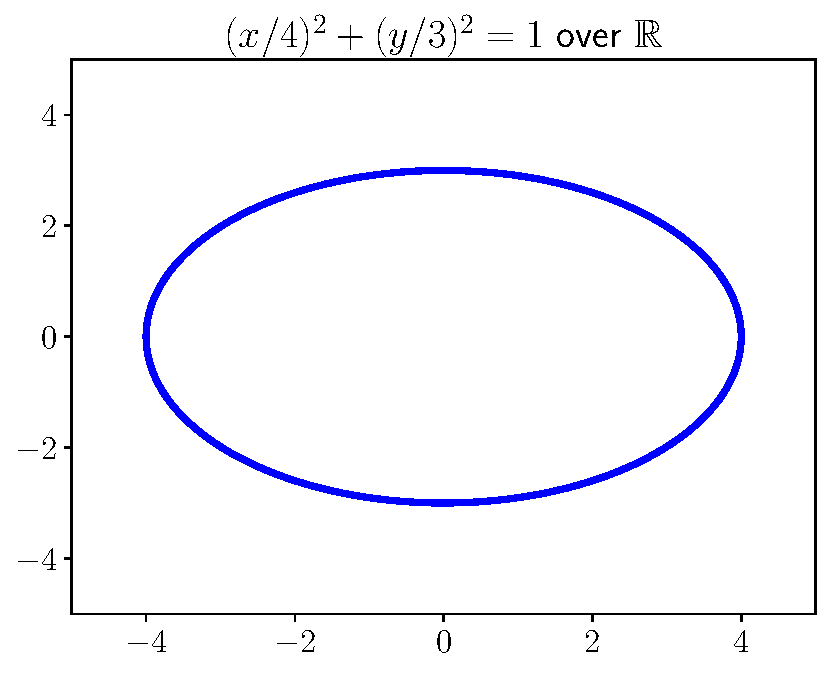
\includegraphics[width=10cm]{plots/ellipse/ellipse_reals_4_3.pdf}
    \caption[Plot of an ellipse over the reals]{Here
        is a plot of an ellipse over $\R$.
        Ellipses are \emph{not} \glspl{elliptic curve}.}
    \label{fig:ellipse_plot}
\end{figure}


Even though \glspl{elliptic curve} are not ellipses,
they are useful for jumping into our discussion of \glspl{elliptic curve}.
Ellipses describe a collection of points which satisfy a polynomial equation;
in this case, a particular quadratic equation.
Additionally, we have some notion of geometry by looking
at the points which satisfy the equation.
\Glspl{elliptic curve} arise in a similar manner but from a different polynomial
equation.

We will never mention ellipses again.

\subsection{Elliptic Curves over the Reals}

We will now look at some examples of \glspl{elliptic curve} over $\R$.
To do this, we will look at $\parens{x,y}\in\R^{2}$ which satisfy

\begin{equation}
    y^{2} = x^{3} + ax + b
    \label{eq:ec_reals}
\end{equation}

\noindent
for $a,b\in\R$.
Example plots can be found in Figures~\ref{fig:ec_real_plots_1}
and \ref{fig:ec_real_plots_2}.

\begin{figure}[p]
\centering
    \begin{subfigure}[t]{0.45\textwidth}
    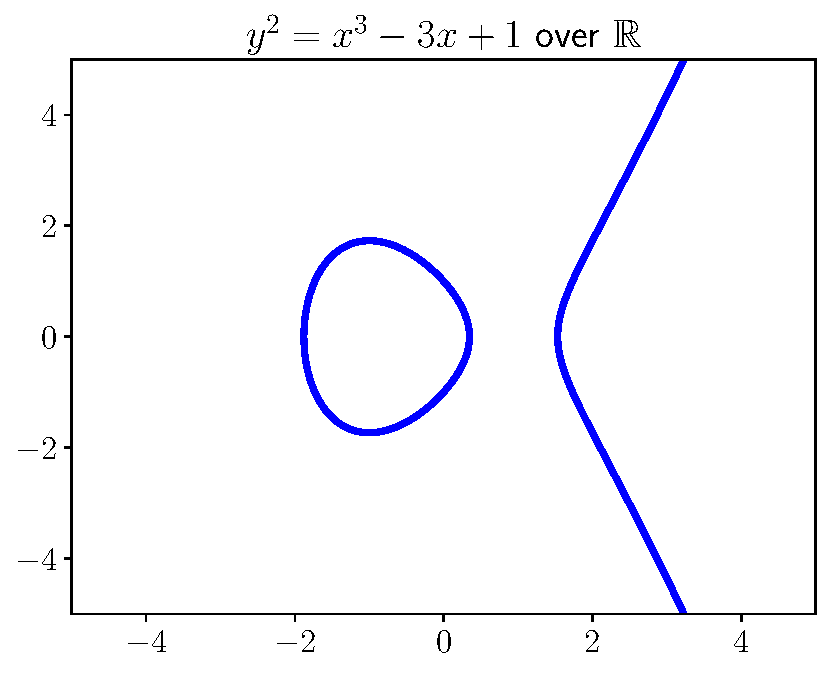
\includegraphics[width=\textwidth]{plots/ec_reals/ec_reals_n3_1.pdf}
    \end{subfigure}
    \begin{subfigure}[t]{0.45\textwidth}
    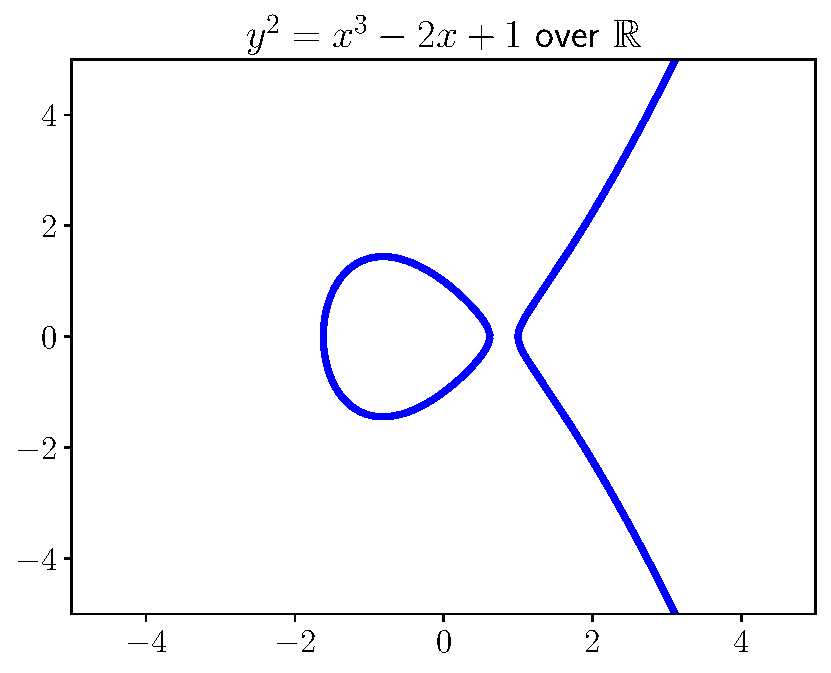
\includegraphics[width=\textwidth]{plots/ec_reals/ec_reals_n2_1.pdf}
    \end{subfigure}

    \begin{subfigure}[t]{0.45\textwidth}
    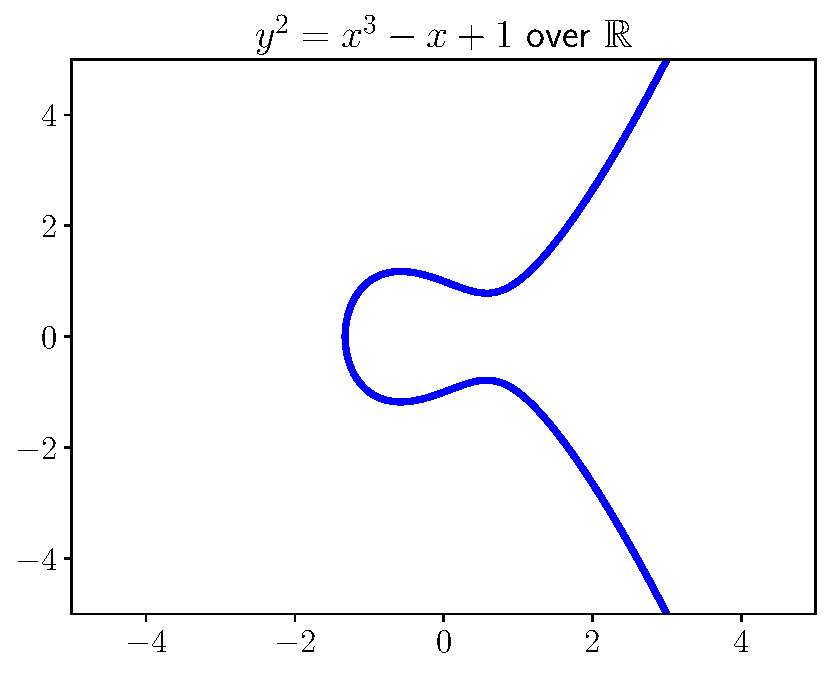
\includegraphics[width=\textwidth]{plots/ec_reals/ec_reals_n1_1.pdf}
    \end{subfigure}
    \begin{subfigure}[t]{0.45\textwidth}
    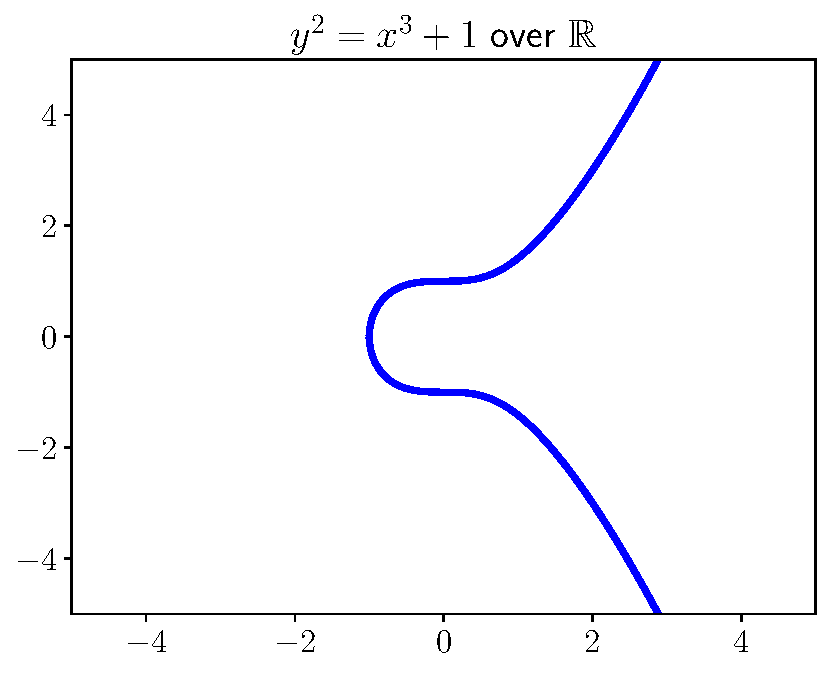
\includegraphics[width=\textwidth]{plots/ec_reals/ec_reals_0_1.pdf}
    \end{subfigure}

    \begin{subfigure}[t]{0.45\textwidth}
    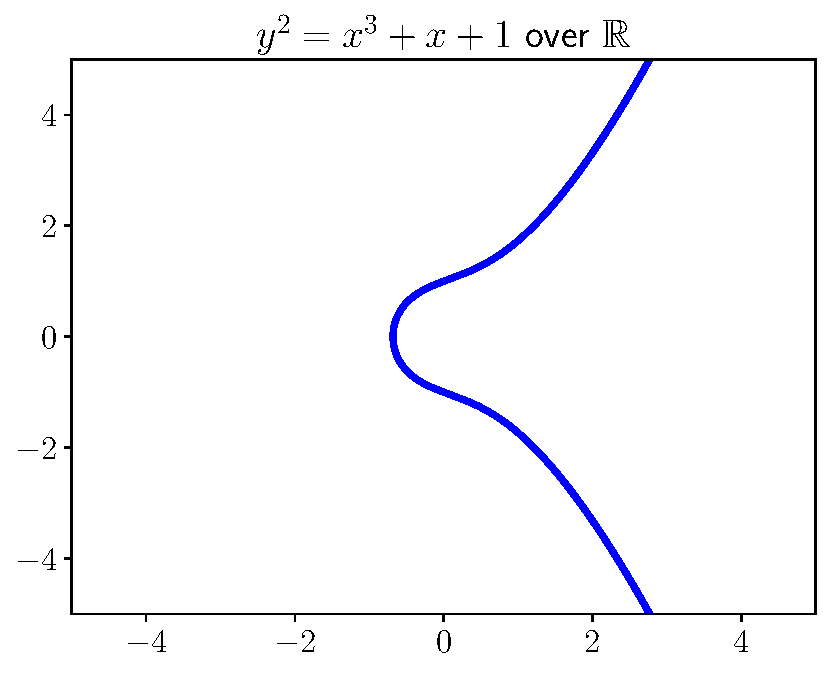
\includegraphics[width=\textwidth]{plots/ec_reals/ec_reals_1_1.pdf}
    \end{subfigure}
    \begin{subfigure}[t]{0.45\textwidth}
    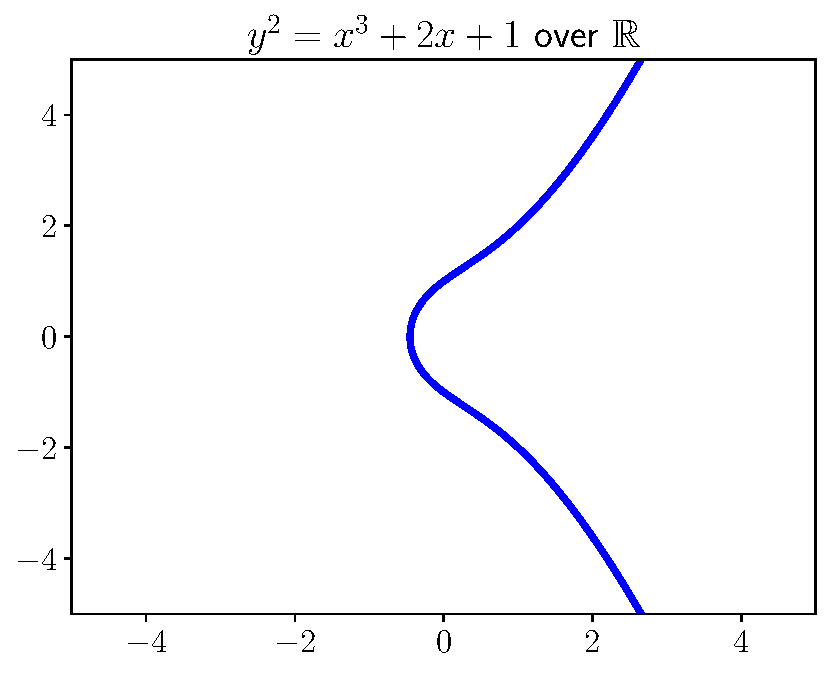
\includegraphics[width=\textwidth]{plots/ec_reals/ec_reals_2_1.pdf}
    \end{subfigure}
    \caption[Plots of elliptic curves over the reals 1]{Here
        are plots of \glspl{elliptic curve} over $\R$.
        The $\parens{x,y}$ points satisfy the equation
        $y^{2} = x^{3} + ax + b$;
        we vary $a$ and hold $b$ constant.}
    \label{fig:ec_real_plots_1}
\end{figure}

\begin{figure}[p]
\centering
    \begin{subfigure}[t]{0.45\textwidth}
    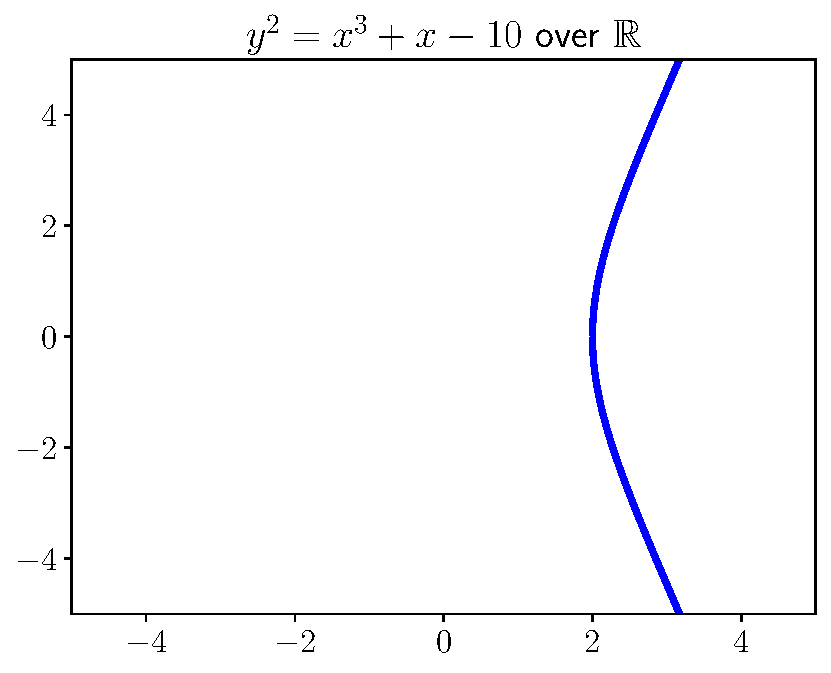
\includegraphics[width=\textwidth]{plots/ec_reals/ec_reals_1_n10.pdf}
    \end{subfigure}
    \begin{subfigure}[t]{0.45\textwidth}
    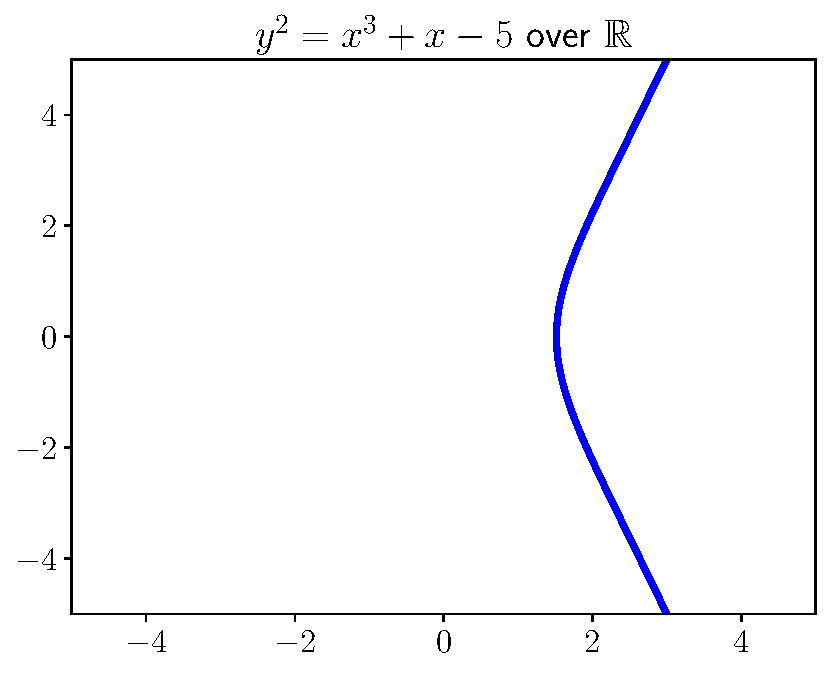
\includegraphics[width=\textwidth]{plots/ec_reals/ec_reals_1_n5.pdf}
    \end{subfigure}

    \begin{subfigure}[t]{0.45\textwidth}
    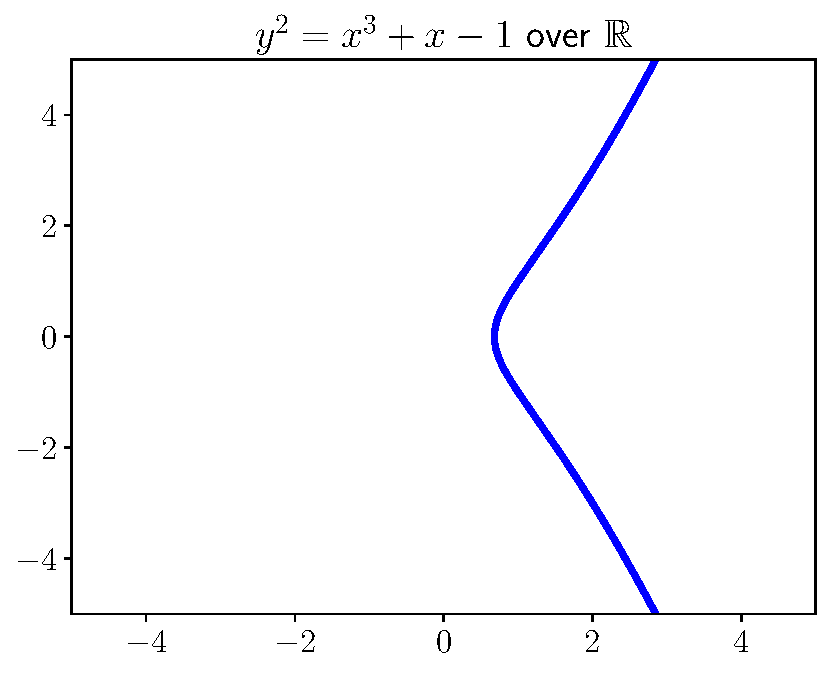
\includegraphics[width=\textwidth]{plots/ec_reals/ec_reals_1_n1.pdf}
    \end{subfigure}
    \begin{subfigure}[t]{0.45\textwidth}
    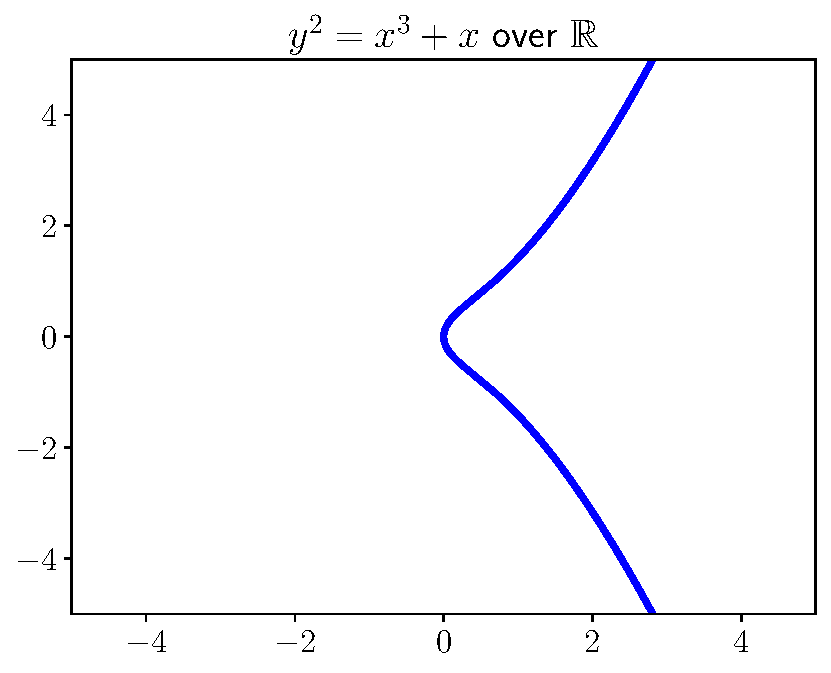
\includegraphics[width=\textwidth]{plots/ec_reals/ec_reals_1_0.pdf}
    \end{subfigure}

    \begin{subfigure}[t]{0.45\textwidth}
    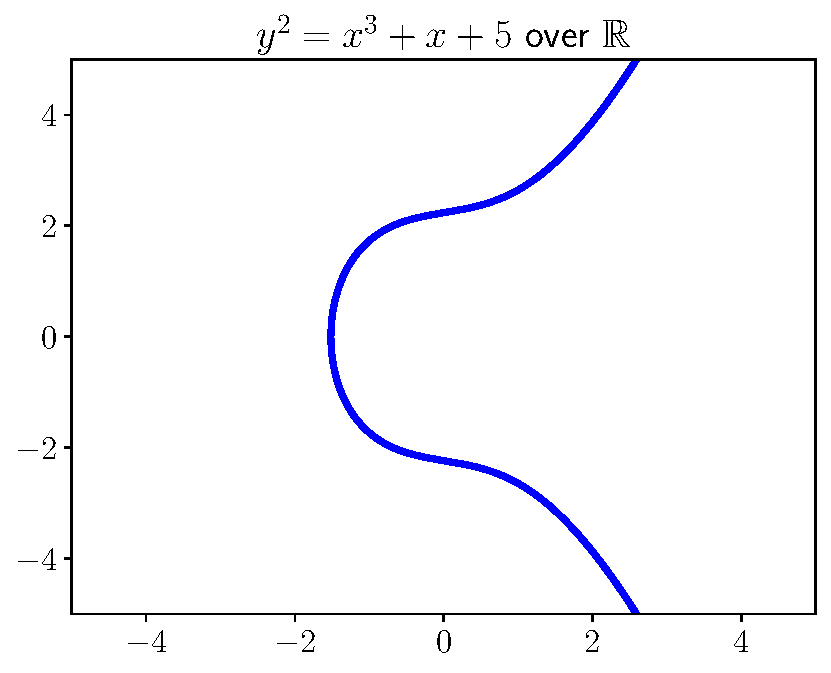
\includegraphics[width=\textwidth]{plots/ec_reals/ec_reals_1_5.pdf}
    \end{subfigure}
    \begin{subfigure}[t]{0.45\textwidth}
    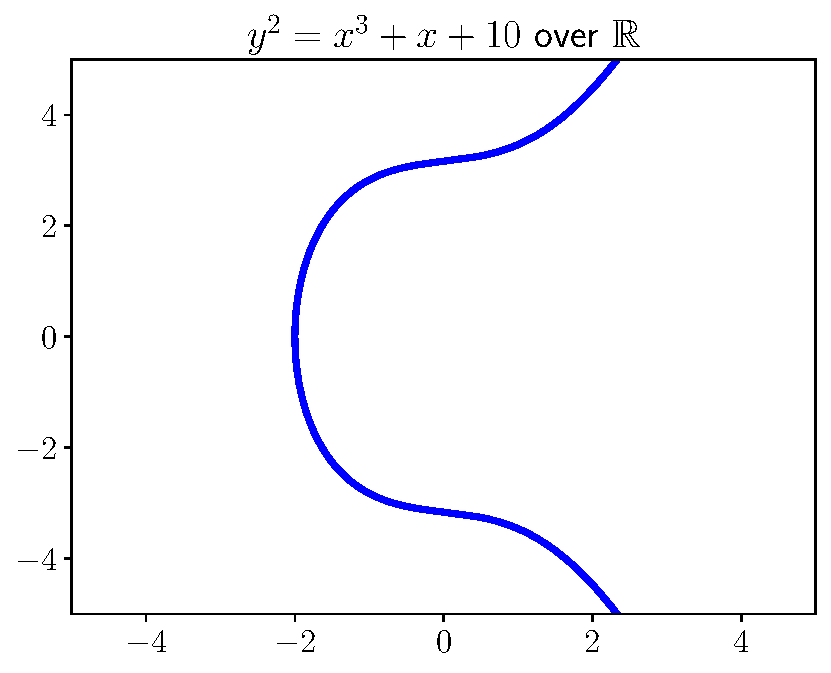
\includegraphics[width=\textwidth]{plots/ec_reals/ec_reals_1_10.pdf}
    \end{subfigure}
    \caption[Plots of elliptic curves over the reals 2]{Here
        are additional plots of \glspl{elliptic curve} over $\R$.
        The $\parens{x,y}$ points satisfy the equation
        $y^{2} = x^{3} + ax + b$;
        we vary $b$ and hold $a$ constant.}
    \label{fig:ec_real_plots_2}
\end{figure}


First, we notice the symmetry about the $x$-axis.
We expect this symmetry because we have
$y^{2} = \cdots$ in Eq.~\eqref{eq:ec_reals}.
Furthermore, we note that by changing $a$ and $b$, we change characteristics
of the curve.
In Figure~\ref{fig:ec_real_plots_1} we vary $a$;
in Figure~\ref{fig:ec_real_plots_2} we vary $b$.

\subsection{Elliptic Curve Addition}
\label{ssec:math_elliptic_addition}

We previously stated that \glspl{elliptic curve} give more freedom
to construct \glspl{group}.
At this point, it is not clear what the \gls{group} structure is,
as we have just seen the equation defining the curve
and looked at some plots.

We now define addition on points of \glspl{elliptic curve}.
As before, we will be looking at points $\parens{x,y}$ which satisfy

\begin{equation}
    y^{2} = x^{3} + ax + b.
    \label{eq:ec_addition}
\end{equation}

\noindent
We also include a special point $\mathcal{O}$;
this point is the additive identity on the \gls{elliptic curve}.
Thus, for any point $P$ on the \gls{elliptic curve},
we have

\begin{equation}
    \mathcal{O} + P = P.
\end{equation}

We suppose that $P = \parens{x_{1},y_{1}}$
and $Q = \parens{x_{2},y_{2}}$ with $P\ne\mathcal{O}$
and $Q\ne\mathcal{O}$;
that is, $P$ and $Q$ are points on the \gls{elliptic curve} which
are not the identity element.
We want to compute $R$ such that

\begin{equation}
    P + Q = R.
\end{equation}

\noindent
We have a few different cases to consider:

\begin{itemize}
\item Case 1: $x_{1}\ne x_{2}$ and $y_{1}\ne y_{2}$

This the general case.
We set

\begin{align}
    s &\mathDef{} \frac{y_{2}-y_{1}}{x_{2}-x_{1}} \nonumber\\
    x_{3} &\mathDef{} s^{2} - x_{1} - x_{2} \nonumber\\
    y_{3} &\mathDef{} s\parens{x_{1} - x_{3}} - y_{1}.
\end{align}

\noindent
In this case, we set

\begin{equation}
    R \mathDef{} \parens{x_{3},y_{3}}.
\end{equation}

\item Case 2: $x_{1} = x_{2}$ and $y_{1}\ne y_{2}$

In this case, we have $Q = -P$, so

\begin{equation}
    R \mathDef{} \mathcal{O}.
\end{equation}

\item Case 3: $x_{1} = x_{2}$ and $y_{1} = y_{2}$

In this case, we need to add a point to itself;
this is also called \emph{point doubling},
and we want to compute $P + P = R$.
We set

\begin{align}
    s &\mathDef{} \frac{3x_{1}^{2} + a}{2y_{1}} \nonumber\\
    x_{3} &\mathDef{} s^{2} - 2x_{1} \nonumber\\
    y_{3} &\mathDef{} s\parens{x_{1} - x_{3}} - y_{1}.
\end{align}

\noindent
In this case, we set

\begin{equation}
    R \mathDef{} \parens{x_{3},y_{3}}.
\end{equation}
\end{itemize}

\noindent
This, when including addition by the identity element,
is the entire addition formula;
one reference is \cite[Proposition~9.70]{IntroModernCrypto}.
Although we have not shown it, \glspl{elliptic curve}
form \glspl{abelian group};
this means that

\begin{equation}
    P + Q = Q + P
\end{equation}

\noindent
for all points $P$ and $Q$.

As mentioned above, if we have $P = \parens{x,y}$,
the additive inverse $-P$ satisfies

\begin{equation}
    -P \mathDef{} \parens{x,-y}.
\end{equation}

\noindent
Naturally, we have

\begin{equation}
    P + \parens{-P} = \mathcal{O}.
\end{equation}

The addition law described here depends on the particular form
of \gls{elliptic curve}.
Additional types of \glspl{elliptic curve} are discussed below,
and the addition formula described here does not always apply.
In fact, due to the nature of the addition formula
(involving conditional checks and different paths for different points),
certain \gls{ecc} (ECC) algorithms specifically
choose a different form of \gls{elliptic curve}.
The branch logic required to implement the above addition formula
will leak secret information if it is not
carefully implemented~\cite{brumley2011remote}.

Plots for elliptic curve addition in
Examples~\ref{example:ec_real_addition_1}
and \ref{example:ec_real_addition_2}
can be found in Figure~\ref{fig:ec_real_plots_addition}.

\begin{figure}[p]
\centering
    \begin{subfigure}[t]{\textwidth}
        \centering
    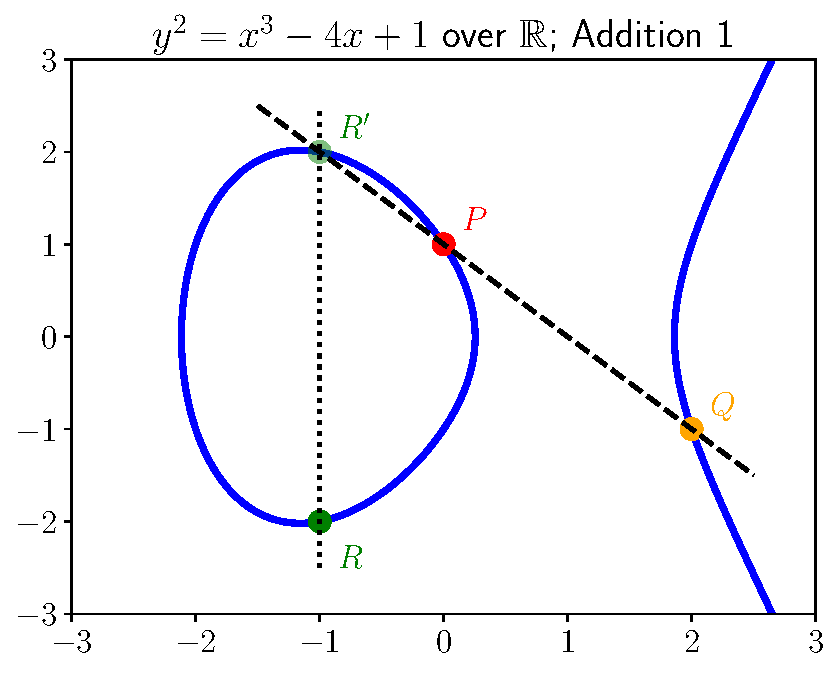
\includegraphics[width=0.70\textwidth]{plots/ec_reals/ec_reals_addition_1.pdf}
    \caption{Plot of elliptic curve addition over $\R$ for
        Example~\ref{example:ec_real_addition_1};
        this is an example of adding distinct points.
        We have
        $\textcolor{red}{P} + \textcolor{orange}{Q} =
        \textcolor[rgb]{0,0.33,0}{R}$.
        This figure shows
        $\textcolor{red}{\parens{0,1}} + \textcolor{orange}{\parens{2,-1}}
        = \textcolor[rgb]{0,0.33,0}{\parens{-1,-2}}$.}
    \label{fig:ec_real_plots_addition_1}
    \end{subfigure}

    \begin{subfigure}[t]{\textwidth}
        \centering
    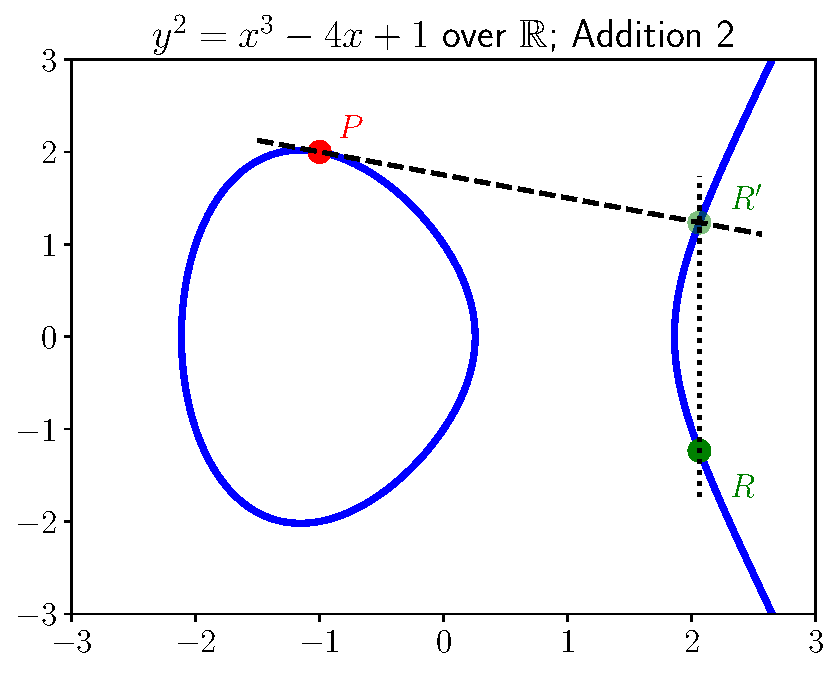
\includegraphics[width=0.70\textwidth]{plots/ec_reals/ec_reals_addition_2.pdf}
    \caption{Plot of elliptic curve addition over $\R$ for
        Example~\ref{example:ec_real_addition_2};
        this is an example of \emph{point doubling}.
        We have
        $\textcolor{red}{P} + \textcolor{red}{P} =
        \textcolor[rgb]{0,0.33,0}{R}$.
        This may also be written as
        $2\cdot\textcolor{red}{P} = \textcolor[rgb]{0,0.33,0}{R}$.
        This figure shows
        $2\cdot\textcolor{red}{\parens{-1,2}}
        = \textcolor[rgb]{0,0.33,0}{\parens{\frac{33}{16},-\frac{79}{64}}}$.}
    \label{fig:ec_real_plots_addition_2}
    \end{subfigure}

\caption[Plots of elliptic curve addition over the reals]{Here
    we plot elliptic curve addition over $\R$
    for Examples~\ref{example:ec_real_addition_1}
    and \ref{example:ec_real_addition_2}.
    Figure~\ref{fig:ec_real_plots_addition_1} shows the addition
    of distinct points while
    Figure~\ref{fig:ec_real_plots_addition_2} shows the addition
    of repeated points (point doubling).}
\label{fig:ec_real_plots_addition}
\end{figure}


\begin{example}[Elliptic Curve Addition over Reals 1]
\label{example:ec_real_addition_1}
We now look at addition on the \gls{elliptic curve}

\begin{equation}
    E: y^{2} = x^{3} - 4x + 1
\end{equation}

\noindent
over $\R$.
We want to add the two points

\begin{align}
    \textcolor{red}{P} &= \parens{0,1} \nonumber\\
    \textcolor{orange}{Q} &= \parens{2,-1}.
\end{align}

\noindent
Using the addition formula, we find

\begin{align}
    s &= -1 \nonumber\\
    x_{3} &= -1 \nonumber\\
    y_{3} &= -2.
\end{align}

\noindent
This gives us the point

\begin{equation}
    \textcolor[rgb]{0,0.33,0}{R} = \parens{-1,-2}.
\end{equation}

\noindent
Thus, we have

\begin{equation}
    \textcolor{red}{\parens{0,1}} + \textcolor{orange}{\parens{2,-1}}
    = \textcolor[rgb]{0,0.33,0}{\parens{-1,-2}}.
\end{equation}

\noindent
See Figure~\ref{fig:ec_real_plots_addition_1}
for a plot.

To understand how $\textcolor[rgb]{0,0.33,0}{R}$ is determined,
we look at the line connecting
$\textcolor{red}{P}$ and $\textcolor{orange}{Q}$.
This line will intersect the \gls{elliptic curve} at another point
$\textcolor[rgb]{0,0.33,0}{R'}$;
it can be shown that this will always happen.
The point $\textcolor[rgb]{0,0.33,0}{R}$ is defined to be
the reflection of $\textcolor[rgb]{0,0.33,0}{R'}$
across the $x$-axis.
\end{example}

\begin{example}[Elliptic Curve Addition over Reals 2]
\label{example:ec_real_addition_2}
We use the same \gls{elliptic curve} in
Example~\ref{example:ec_real_addition_1}:

\begin{equation}
    E: y^{2} = x^{3} - 4x + 1
\end{equation}

\noindent
over $\R$.

In this example, we look at adding a point to itself;
this is also called \emph{point doubling}.
In this case, we have the point

\begin{equation}
    \textcolor{red}{P} = \parens{-1,2}.
\end{equation}

\noindent
We see

\begin{align}
    s &= -\frac{1}{4} \nonumber\\
    x_{3} &= \frac{33}{16} \nonumber\\
    y_{3} &= -\frac{79}{64}.
\end{align}

\noindent
This gives us the point

\begin{equation}
    \textcolor[rgb]{0,0.33,0}{R} = \parens{\frac{33}{16},-\frac{79}{64}}.
\end{equation}

\noindent
Thus, we have

\begin{equation}
    \textcolor{red}{\parens{-1,2}} + \textcolor{red}{\parens{-1,2}}
    = \textcolor[rgb]{0,0.33,0}{\parens{\frac{33}{16},-\frac{79}{64}}}.
\end{equation}

\noindent
This may also be written as

\begin{equation}
    2\cdot\textcolor{red}{\parens{-1,2}}
    = \textcolor[rgb]{0,0.33,0}{\parens{\frac{33}{16},-\frac{79}{64}}}.
\end{equation}

\noindent
See Figure~\ref{fig:ec_real_plots_addition_2}
for a plot.

To understand how $\textcolor[rgb]{0,0.33,0}{R}$ is determined,
we now look at the tangent line of $\textcolor{red}{P}$
on the \gls{elliptic curve}.
This line will intersect the \gls{elliptic curve} at another point
$\textcolor[rgb]{0,0.33,0}{R'}$;
it can be shown that this will always happen.
The point $\textcolor[rgb]{0,0.33,0}{R}$ is defined to be
the reflection of $\textcolor[rgb]{0,0.33,0}{R'}$
across the $x$-axis.
\end{example}


\subsection{Elliptic Curves over General Fields}

We let $K$ be a \gls{field}.
For concreteness, the reader may assume $K = \R$ as before.
We are interested in looking at points $\parens{x,y}\in K^{2}$
which satisfy the equation

\begin{equation}
    E: y^{2} = x^{3} + ax + b
    \label{eq:weierstrass_form}
\end{equation}

\noindent
for $a,b\in K$.
\Glspl{elliptic curve} given in the form in Eq.~\eqref{eq:weierstrass_form}
are said to be in \emph{Weierstrass form}.
We will see other forms of \glspl{elliptic curve}
in Chapter~\ref{ssec:specific_curves}
when we discuss some specific \glspl{elliptic curve} which are used in practice.
The addition law we discussed in
Chapter~\ref{ssec:math_elliptic_addition}
is the same provided the field operations over $K$ are used.

The set of points of an \gls{elliptic curve} along with the addition
formula gives rise to an \gls{abelian group}.
We can look at cyclic subgroups of the \glspl{elliptic curve} to specify
a \gls{dlp}.

We note that there are some technical restrictions on $a$ and $b$
in Eq.~\eqref{eq:weierstrass_form},
but we do not discuss the specifics here.


\subsection{Elliptic Curves over Finite Fields}

We now focus on looking at \glspl{elliptic curve} over the
\gls{field} $\F_{p}$ for prime $p$.
Example plots can be found in Figures~\ref{fig:ec_finite_plots_1}
and \ref{fig:ec_finite_plots_2}
where we look at \glspl{elliptic curve} over $\F_{71}$.

\begin{figure}[p]
\centering
    \begin{subfigure}[t]{0.45\textwidth}
    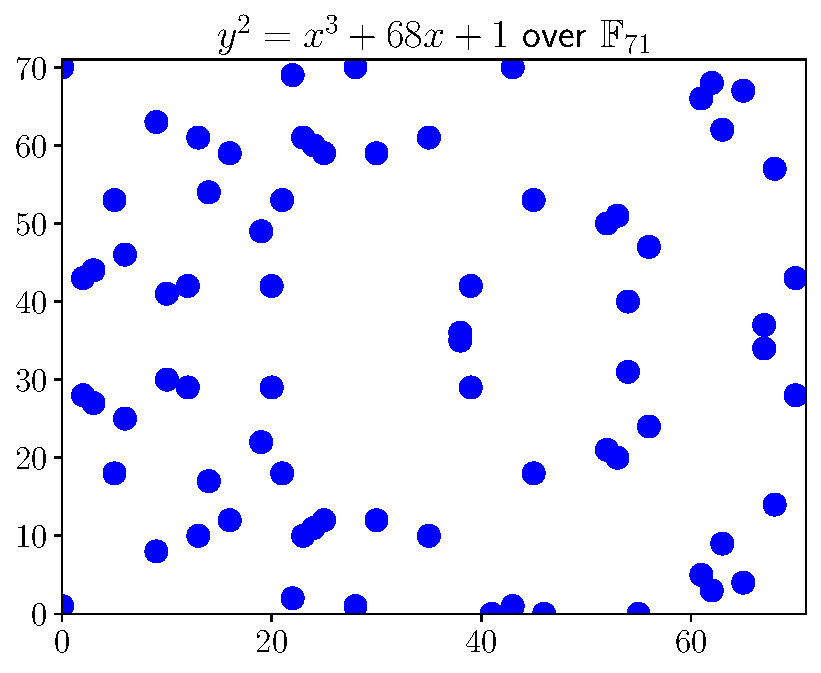
\includegraphics[width=\textwidth]{plots/ec_finite/ec_finite_F_71_68_1.pdf}
    \end{subfigure}
    \begin{subfigure}[t]{0.45\textwidth}
    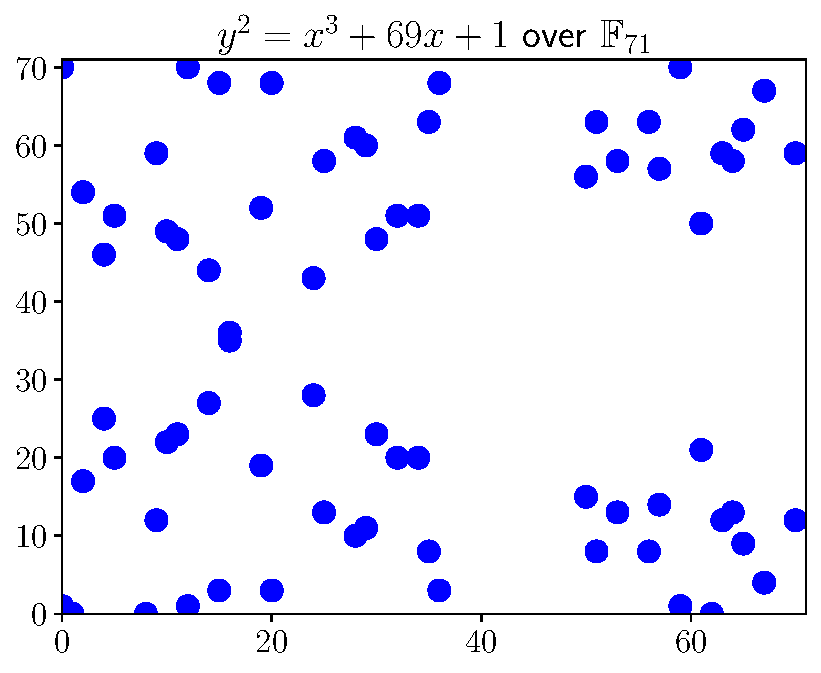
\includegraphics[width=\textwidth]{plots/ec_finite/ec_finite_F_71_69_1.pdf}
    \end{subfigure}

    \begin{subfigure}[t]{0.45\textwidth}
    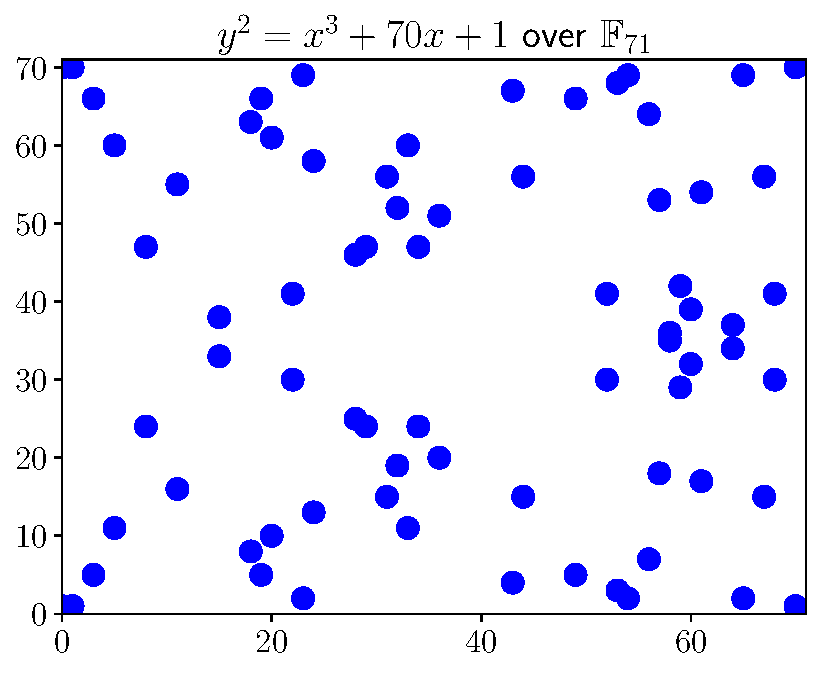
\includegraphics[width=\textwidth]{plots/ec_finite/ec_finite_F_71_70_1.pdf}
    \end{subfigure}
    \begin{subfigure}[t]{0.45\textwidth}
    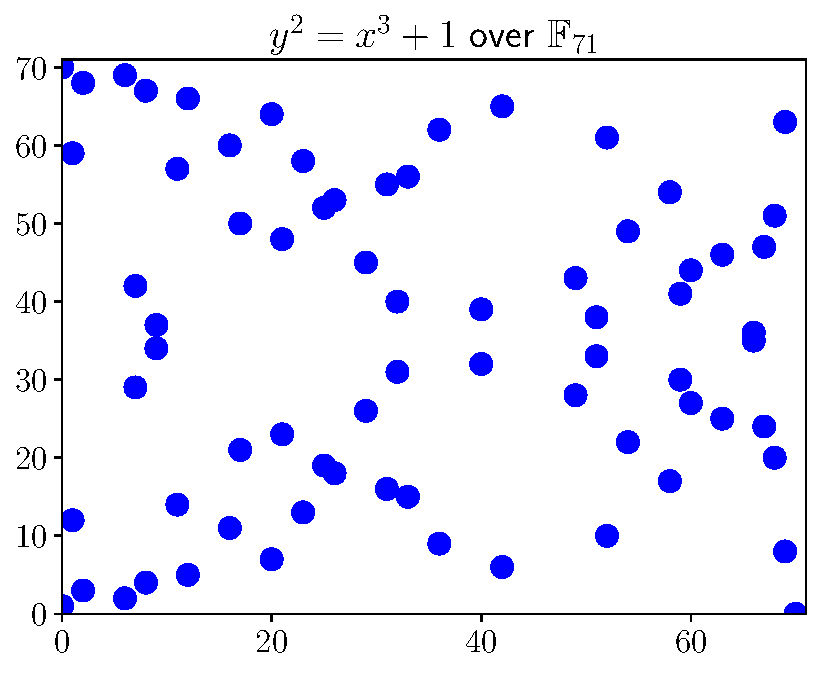
\includegraphics[width=\textwidth]{plots/ec_finite/ec_finite_F_71_0_1.pdf}
    \end{subfigure}

    \begin{subfigure}[t]{0.45\textwidth}
    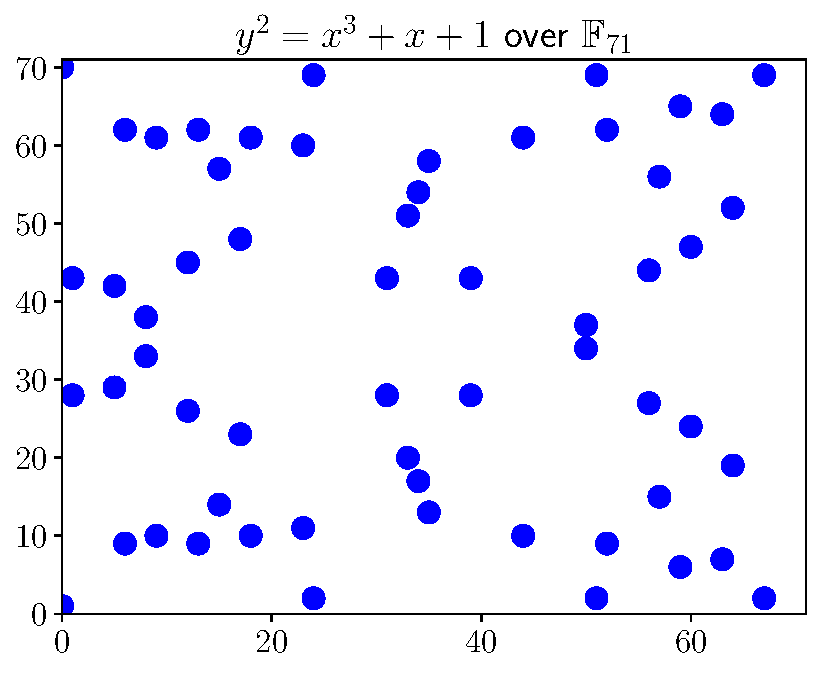
\includegraphics[width=\textwidth]{plots/ec_finite/ec_finite_F_71_1_1.pdf}
    \end{subfigure}
    \begin{subfigure}[t]{0.45\textwidth}
    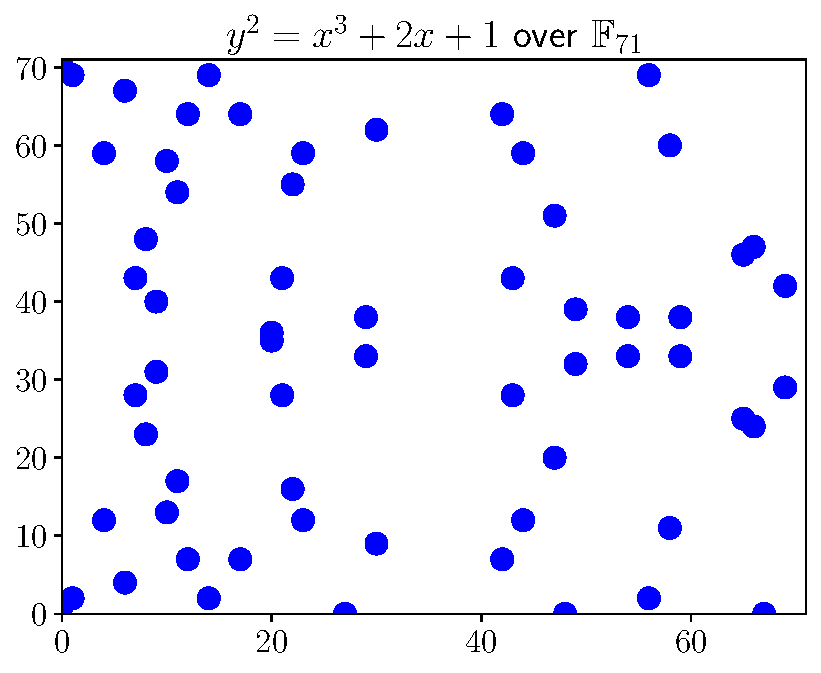
\includegraphics[width=\textwidth]{plots/ec_finite/ec_finite_F_71_2_1.pdf}
    \end{subfigure}
    \caption[Plots of elliptic curves over finite fields 1]{Here
        are plots of \glspl{elliptic curve} over $\F_{71}$.
        Here, we are keeping $b$ constant.}
    \label{fig:ec_finite_plots_1}
\end{figure}

\begin{figure}[p]
\centering
    \begin{subfigure}[t]{0.45\textwidth}
    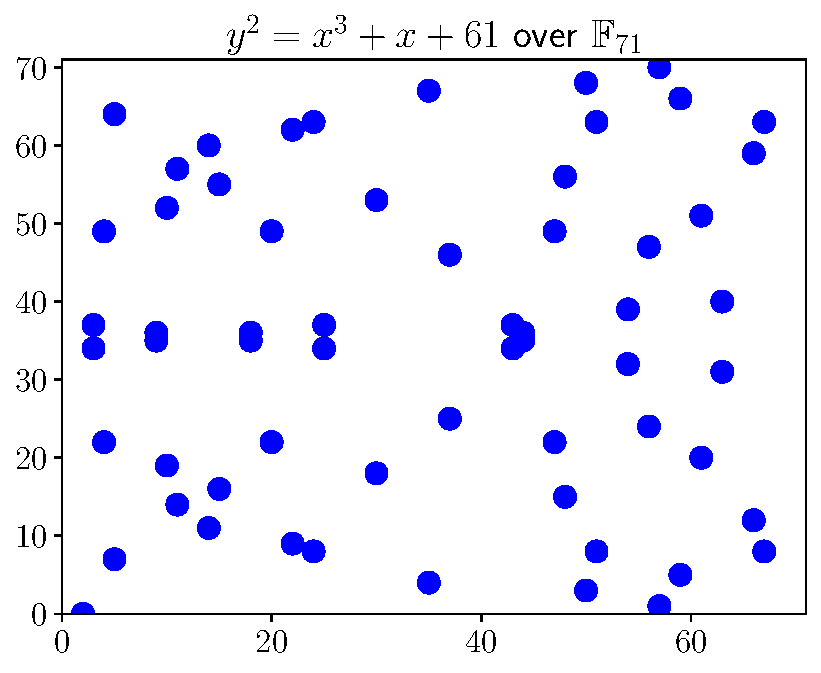
\includegraphics[width=\textwidth]{plots/ec_finite/ec_finite_F_71_1_61.pdf}
    \end{subfigure}
    \begin{subfigure}[t]{0.45\textwidth}
    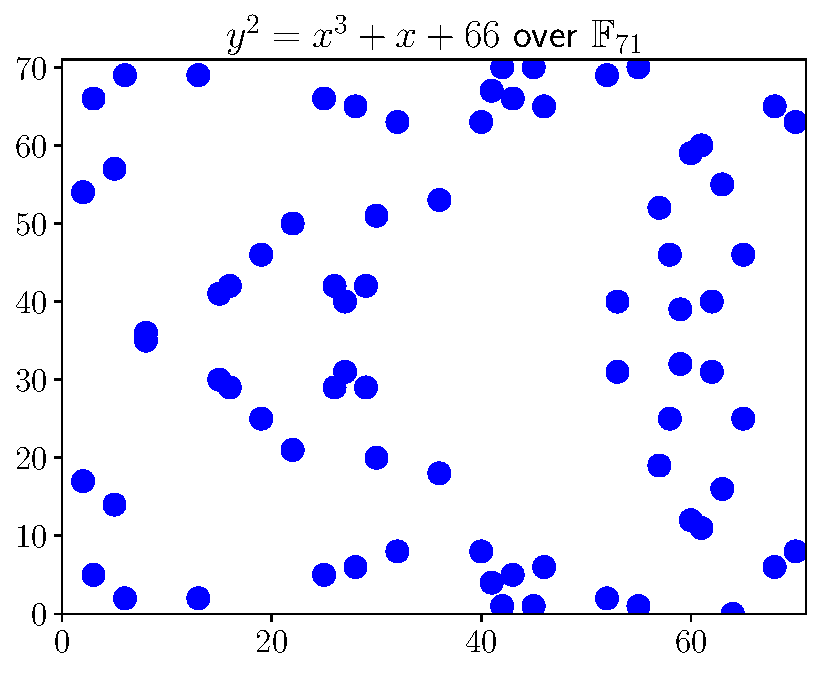
\includegraphics[width=\textwidth]{plots/ec_finite/ec_finite_F_71_1_66.pdf}
    \end{subfigure}

    \begin{subfigure}[t]{0.45\textwidth}
    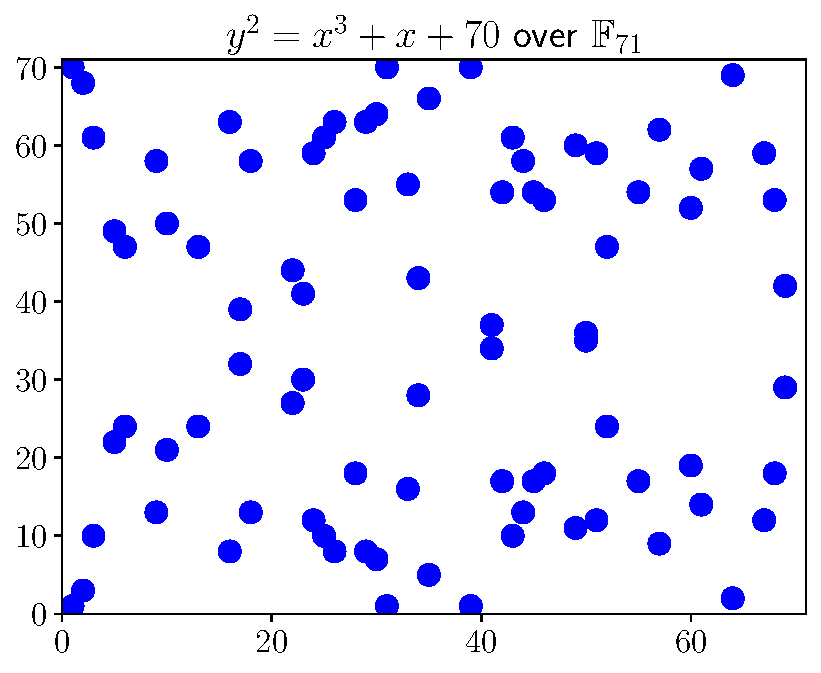
\includegraphics[width=\textwidth]{plots/ec_finite/ec_finite_F_71_1_70.pdf}
    \end{subfigure}
    \begin{subfigure}[t]{0.45\textwidth}
    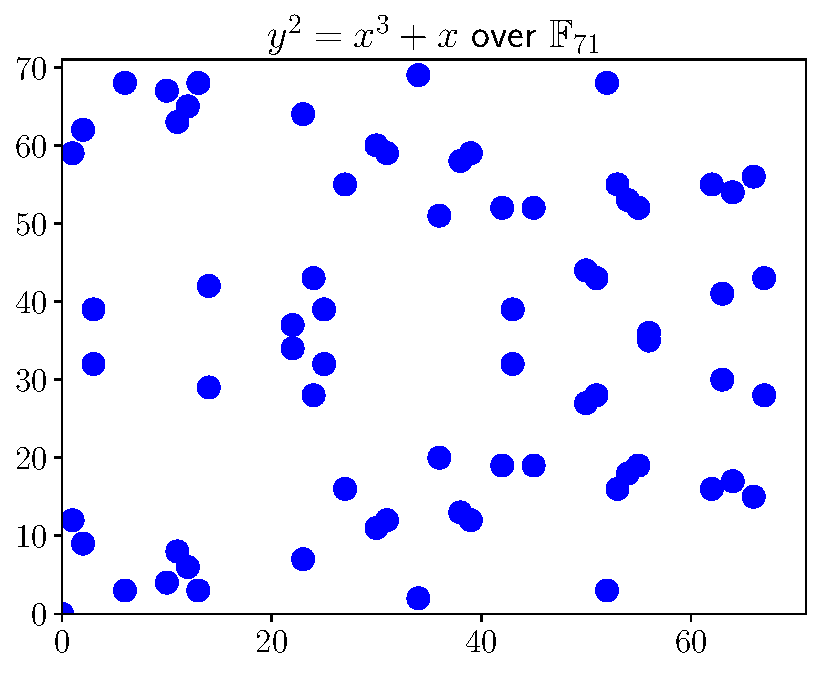
\includegraphics[width=\textwidth]{plots/ec_finite/ec_finite_F_71_1_0.pdf}
    \end{subfigure}

    \begin{subfigure}[t]{0.45\textwidth}
    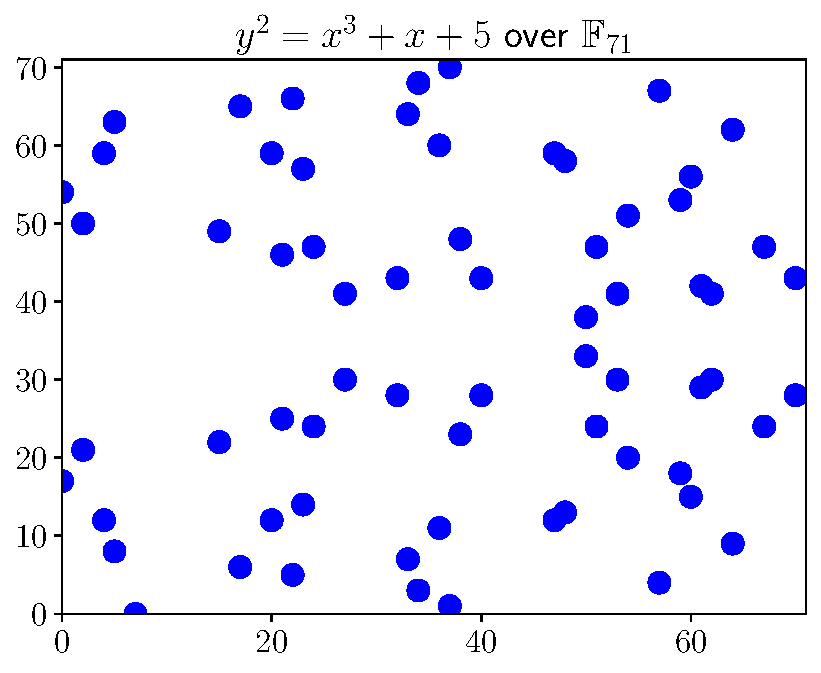
\includegraphics[width=\textwidth]{plots/ec_finite/ec_finite_F_71_1_5.pdf}
    \end{subfigure}
    \begin{subfigure}[t]{0.45\textwidth}
    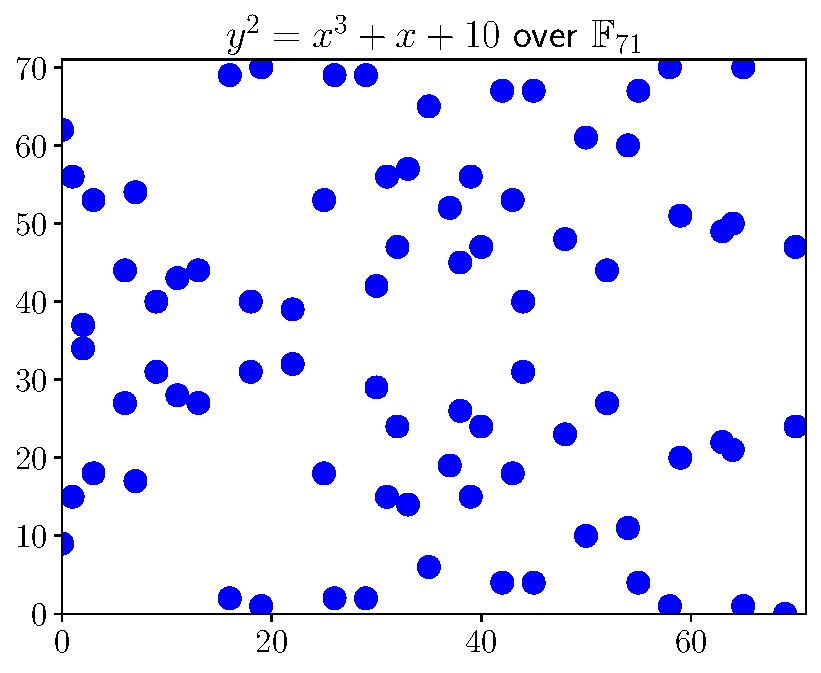
\includegraphics[width=\textwidth]{plots/ec_finite/ec_finite_F_71_1_10.pdf}
    \end{subfigure}
    \caption[Plots of elliptic curves over finite fields 2]{Here
        are additional plots of \glspl{elliptic curve} over $\F_{71}$.
        Here, we are keeping $a$ constant.}
    \label{fig:ec_finite_plots_2}
\end{figure}


The \glspl{elliptic curve} are the ``same'' as the ones in
Figures~\ref{fig:ec_real_plots_1} and \ref{fig:ec_real_plots_2}.
That is, the \emph{equation} describing each of them is the same;
the only difference is that we are now looking for solutions
over a different \gls{field}; we are looking for solutions over $\F_{71}$
rather than $\R$.
By looking at the plots, there does not appear to any relationship
between the parameters and the points on the \gls{elliptic curve}.
We still note the symmetry about the middle of the graph, though.
This comes from the $y^{2} = \cdots$ in the equation definition.

To understand the symmetry about the middle of the graph,
we will spend a bit more time discussing this.
First, we remember that, in our \glspl{finite field}, we have

\begin{equation}
    -y = p-y \mod p.
\end{equation}

\begin{figure}[p]
\centering
    \begin{subfigure}[t]{0.9\textwidth}
    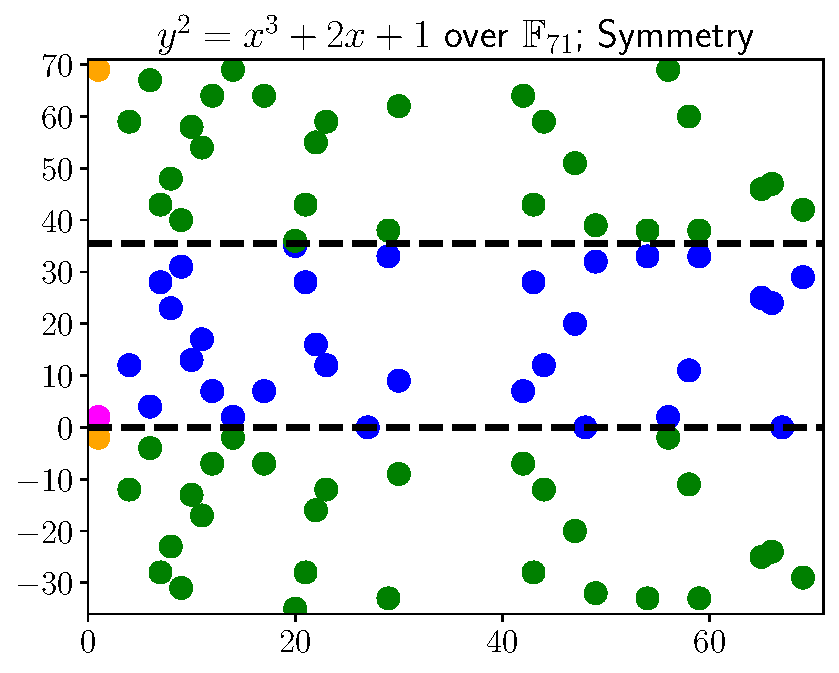
\includegraphics[width=\textwidth]{plots/ec_finite/ec_finite_F_71_2_1_symmetry_base.pdf}
    \caption{Plot with all $y$ values in $\brackets{-p/2,p}$.}
    \label{fig:ec_finite_plots_symmetry_main}
    \end{subfigure}

    \begin{subfigure}[t]{0.45\textwidth}
    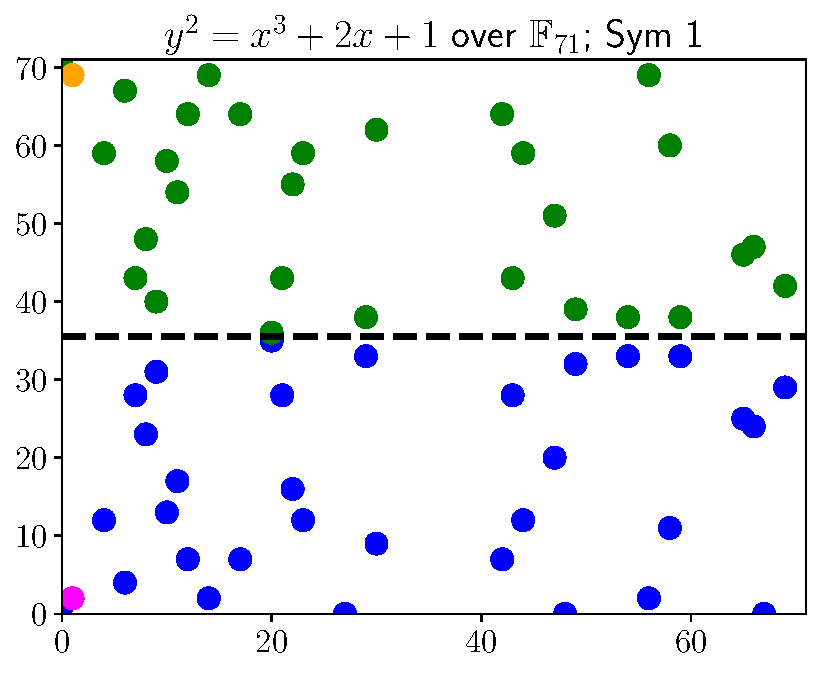
\includegraphics[width=\textwidth]{plots/ec_finite/ec_finite_F_71_2_1_symmetry_1.pdf}
    \caption{Plot with $y$ values in $\brackets{0,p}$.}
    \label{fig:ec_finite_plots_symmetry_1}
    \end{subfigure}
    \begin{subfigure}[t]{0.45\textwidth}
    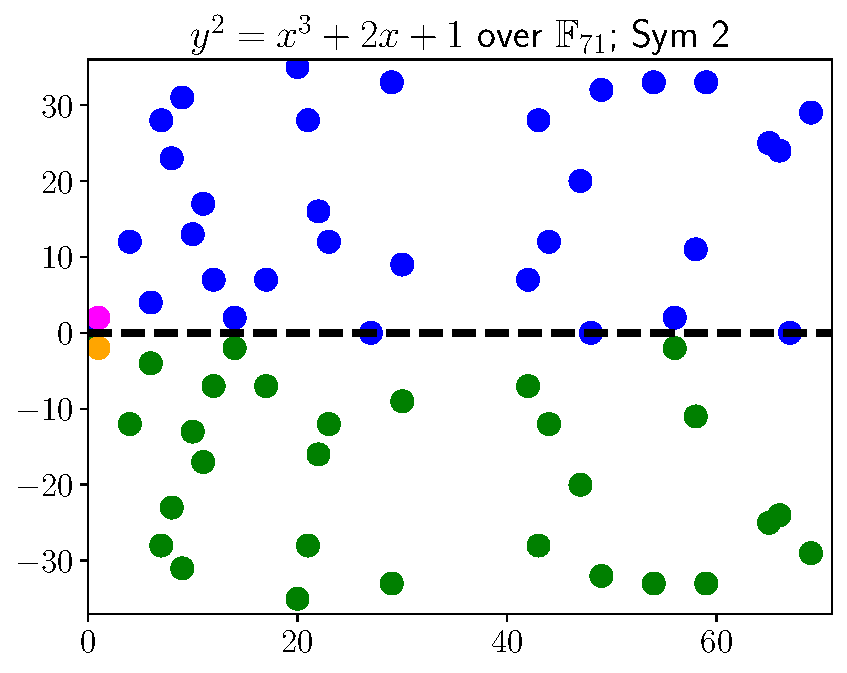
\includegraphics[width=\textwidth]{plots/ec_finite/ec_finite_F_71_2_1_symmetry_2.pdf}
    \caption{Plot with $y$ values in $\brackets{-p/2,p/2}$.}
    \label{fig:ec_finite_plots_symmetry_2}
    \end{subfigure}
\caption[Plots showing symmetry of elliptic curves over finite fields]{Here
    have a plot showing the symmetry of \glspl{elliptic curve} over $\F_{71}$.
    The ``positive'' points are in \textcolor{blue}{blue}
        with $y$-values between $0$ and $p/2$;
    the ``negative'' points are in \textcolor[rgb]{0,0.33,0}{green}
        with $y$-values between $p/2$ and $p$.
    Because $-y = p-y\mod p$,
    the negative points are equivalent to those with $y$ values
    between $-p/2$ and $0$.
    }
\label{fig:ec_finite_plots_symmetry}
\end{figure}


\noindent
To be concrete, we will focus on $y^{2} = x^{3} + 2x + 1$ over $\F_{71}$;
see Figure~\ref{fig:ec_finite_plots_symmetry_main}.
We can see \emph{two} lines of symmetry:
one line at $y=0$; another line at $y=p/2$.
These two lines of symmetry arise from $-y = p-y \mod p$:
we are free in where we put the ``negative'' numbers.
We can place the ``negative'' numbers between $p/2$ and $p$ as seen in
Figure~\ref{fig:ec_finite_plots_symmetry_1};
or we can place the ``negative'' numbers between $-p/2$ and $0$ as seen in
Figure~\ref{fig:ec_finite_plots_symmetry_2}.
In all of our plots, we will use the first convention
and always have plot $y$ values between $0$ and $p$.
Within Figure~\ref{fig:ec_finite_plots_symmetry},
we have a distinguished point $\color{magenta}{\parens{1,2}}$.
The additive inverse of this point is
$\color{orange}{\parens{1,-2}}$.
This is equivalent to $\color{orange}{\parens{1,69}}$
over $\F_{71}$.

All of the previous plots looked at \glspl{elliptic curve} over $\F_{71}$.
Even so, the particular form of \gls{elliptic curve} depends on the
\gls{finite field} as well.
Figure~\ref{fig:ec_finite_plots_fields} includes some plots where
we keep the equation fixed but change the prime $p$.

\begin{figure}[p]
\centering
    \begin{subfigure}[t]{0.45\textwidth}
    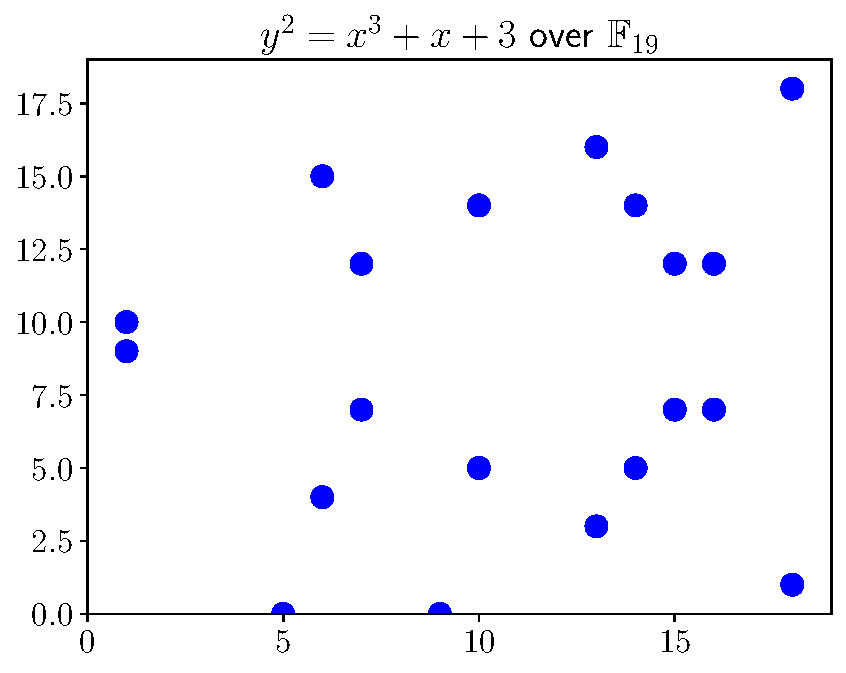
\includegraphics[width=\textwidth]{plots/ec_finite/ec_finite_F_19_1_3.pdf}
    \end{subfigure}
    \begin{subfigure}[t]{0.45\textwidth}
    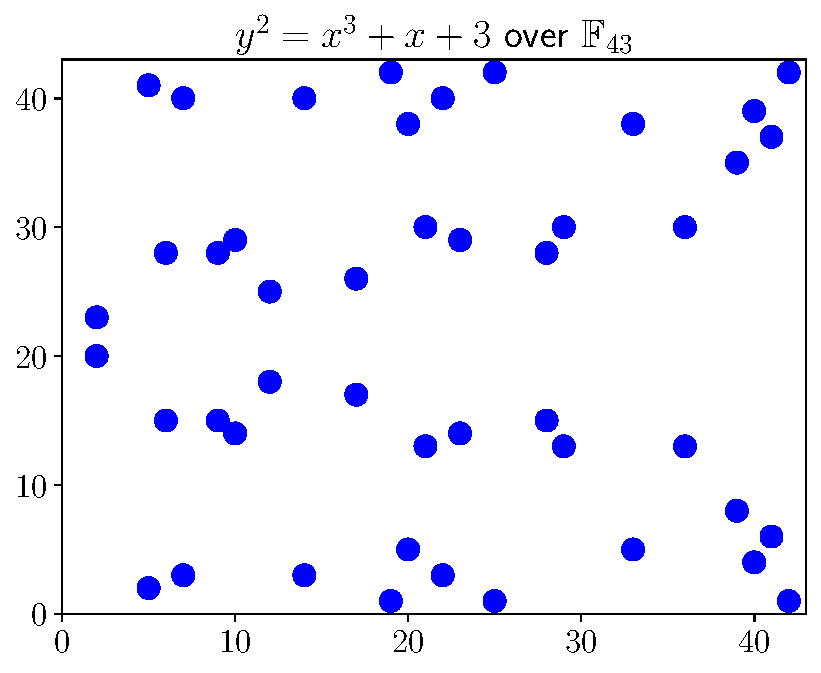
\includegraphics[width=\textwidth]{plots/ec_finite/ec_finite_F_43_1_3.pdf}
    \end{subfigure}

    \begin{subfigure}[t]{0.45\textwidth}
    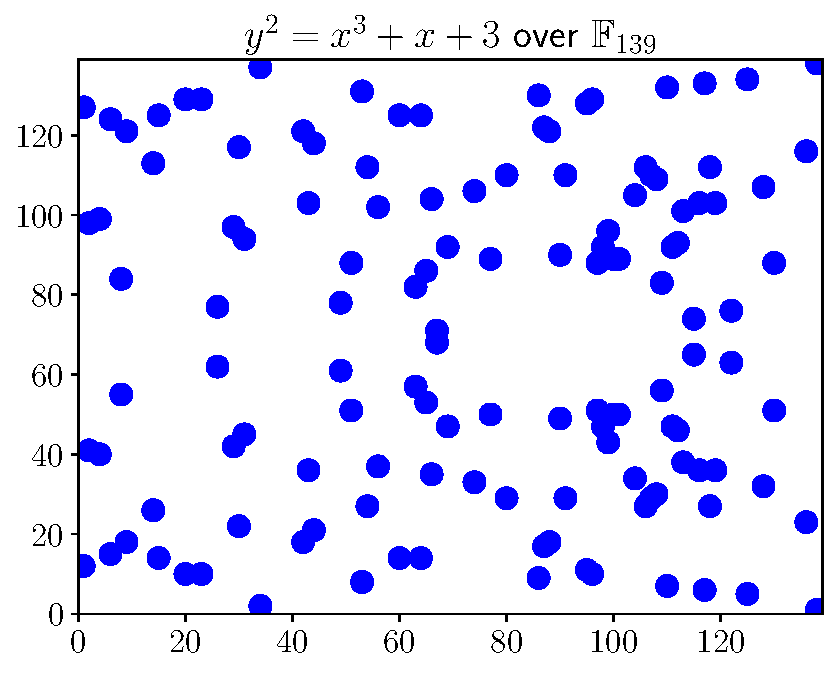
\includegraphics[width=\textwidth]{plots/ec_finite/ec_finite_F_139_1_3.pdf}
    \end{subfigure}
    \begin{subfigure}[t]{0.45\textwidth}
    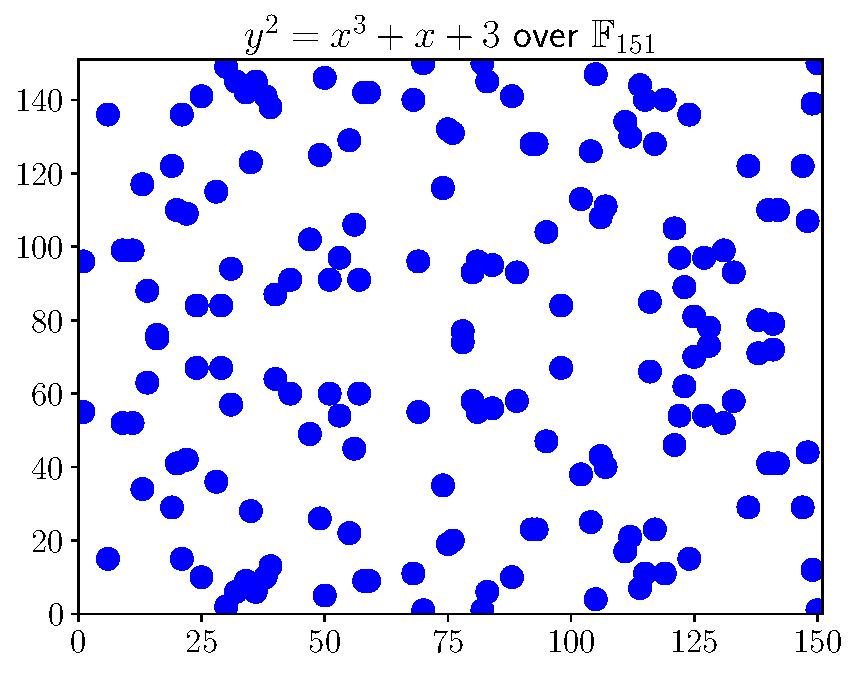
\includegraphics[width=\textwidth]{plots/ec_finite/ec_finite_F_151_1_3.pdf}
    \end{subfigure}

    \begin{subfigure}[t]{0.45\textwidth}
    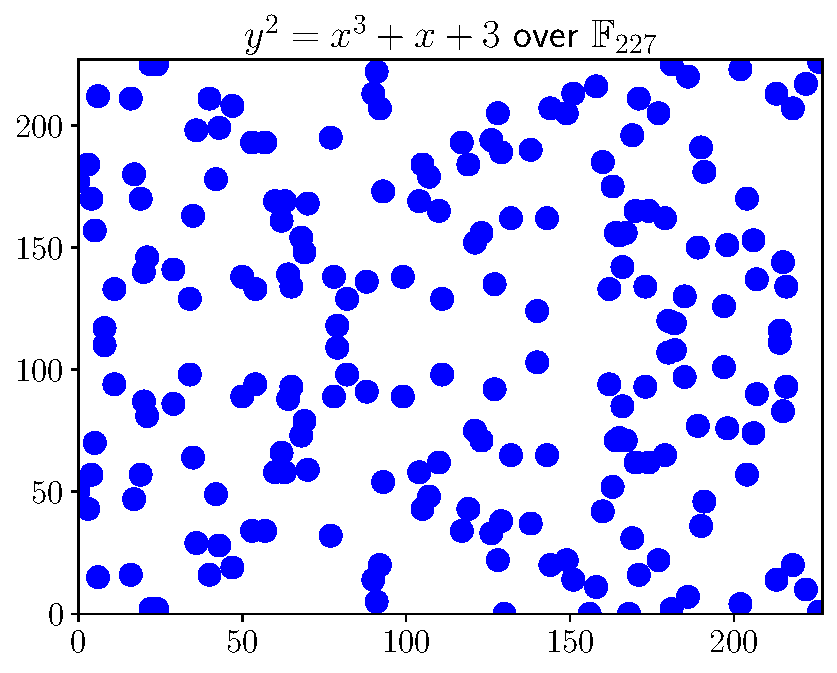
\includegraphics[width=\textwidth]{plots/ec_finite/ec_finite_F_227_1_3.pdf}
    \end{subfigure}
    \begin{subfigure}[t]{0.45\textwidth}
    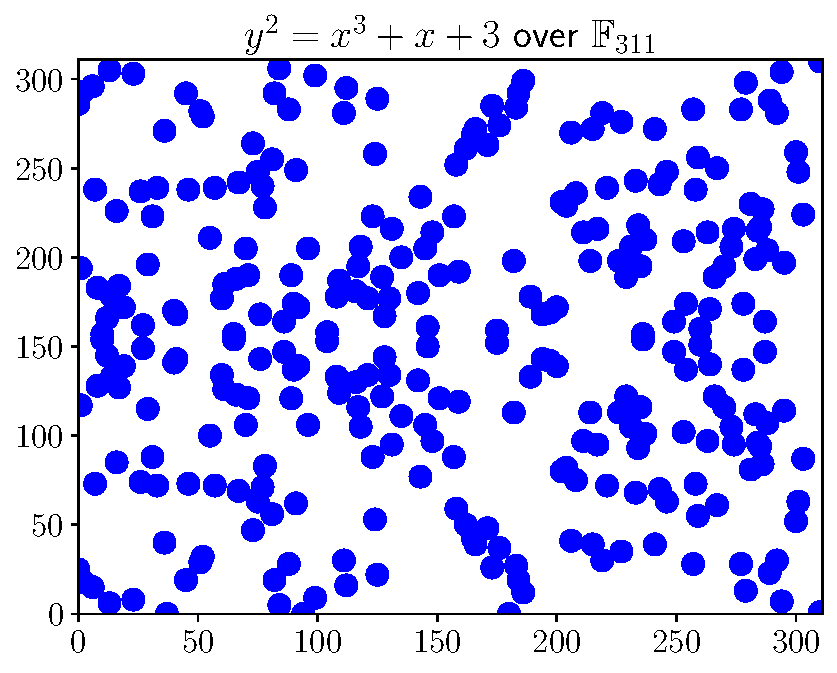
\includegraphics[width=\textwidth]{plots/ec_finite/ec_finite_F_311_1_3.pdf}
    \end{subfigure}
    \caption[Plots of elliptic curves over various finite fields]{Here
        are plots of \glspl{elliptic curve} over $\F_{p}$
        for primes $p\in\braces{19, 43, 139, 151, 227, 311}$.}
    \label{fig:ec_finite_plots_fields}
\end{figure}


We have not talked about methods to determine how many points
are on a specific \gls{elliptic curve}.
There are methods to compute the exact number of
elements on an \gls{elliptic curve},
but we will not discuss them here.
Here is an easy bound on the number of points:

\begin{thm}[{{Hasse's Theorem on Elliptic Curves~\cite[Theorem V.1.1]{AEC}}}]
\label{thm:hasse_bound}
Let $\#E(\F_{p})$ denote the number of elements of an \gls{elliptic curve}
$E/\F_{p}$.
Then we have the following bound:

\begin{equation}
    \abs{\#E(\F_{p}) - \parens{p+1}} \le 2\sqrt{p}.
\end{equation}
\end{thm}

\noindent
This means that the number of points on the \gls{elliptic curve}
$E\parens{\F_{p}}$ is essentially $p$.

We now look at some examples of addition on \glspl{elliptic curve}.
By looking at the points and the \gls{elliptic curve},
there does not appear to be any structure.

\begin{example}[Addition of Elliptic Curves over Finite Fields]
\exampleCodeReference{examples/math\_review/elliptic\_curve\_addition.py}

We will focus on the \gls{elliptic curve}

\begin{equation}
    E: y^{2} = x^{3} + 2x + 1
\end{equation}

\noindent
over $\F_{71}$.

We compute the following values:

\begin{align}
    \parens{17,7} + \parens{20,35} &= \parens{58,60}
        \nonumber\\
    \parens{17,7} + \parens{21,28} &= \parens{65,25}
        \nonumber\\
    \parens{17,7} + \parens{22,16} &= \parens{4,59}
        \nonumber\\
    \parens{17,7} + \parens{23,12} &= \parens{10,58}
        \nonumber\\
    \parens{17,7} + \parens{29,33} &= \parens{8,48}.
\end{align}

\noindent
We plot the results of addition in Figure~\ref{fig:ec_finite_plots_addition}.

\begin{figure}[p]
\centering
    \begin{subfigure}[t]{0.45\textwidth}
    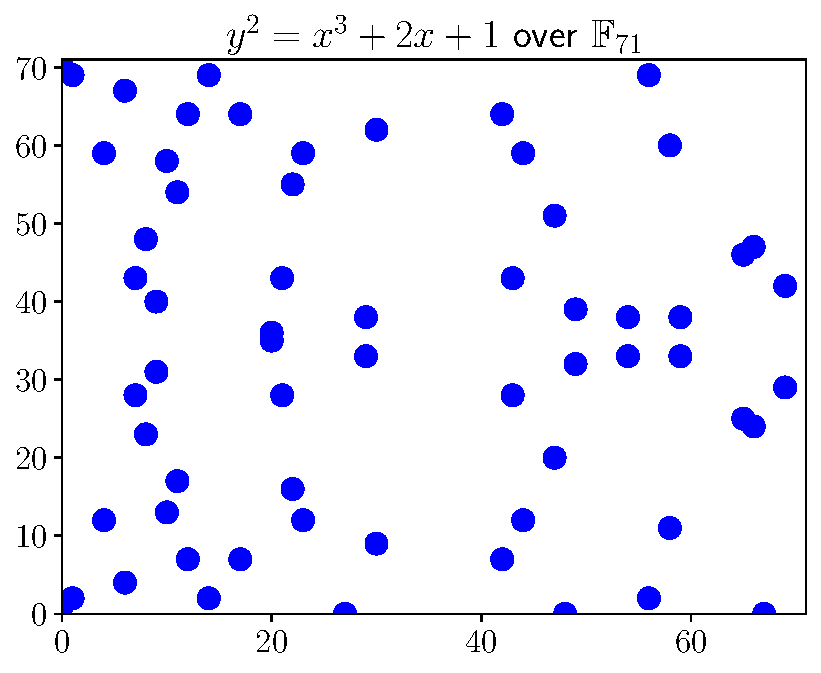
\includegraphics[width=\textwidth]{plots/ec_finite/ec_finite_F_71_2_1_addition_base.pdf}
    \caption{All points on $y^{2} = x^{3} + 2x + 1$ over $\F_{71}$.}
    \end{subfigure}
    \begin{subfigure}[t]{0.45\textwidth}
    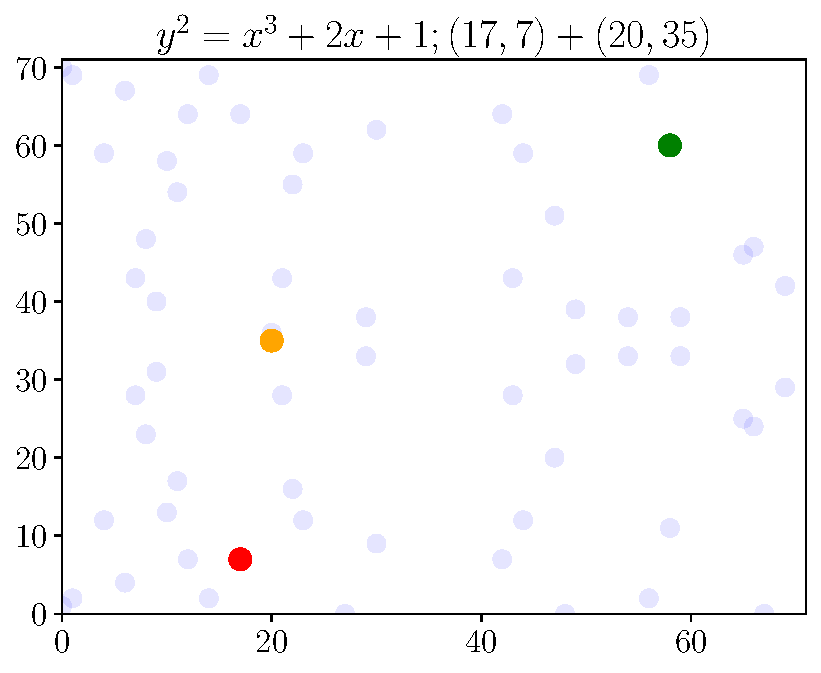
\includegraphics[width=\textwidth]{plots/ec_finite/ec_finite_F_71_2_1_addition_20_35.pdf}
    \caption{$\textcolor{red}{\parens{17,7}}
        + \textcolor{orange}{\parens{20,35}}
        = \textcolor[rgb]{0,0.33,0}{\parens{58,60}}$}
    \end{subfigure}

    \begin{subfigure}[t]{0.45\textwidth}
    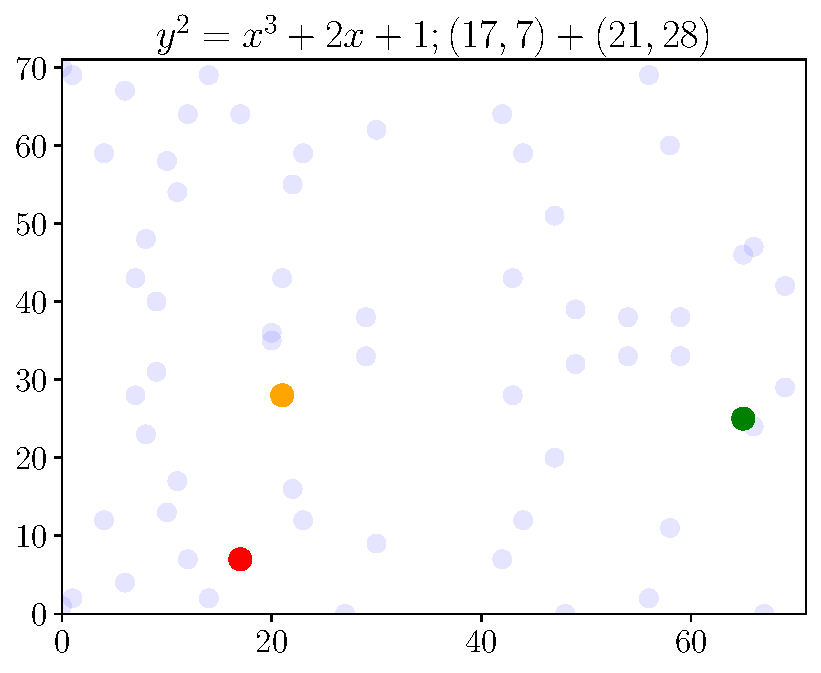
\includegraphics[width=\textwidth]{plots/ec_finite/ec_finite_F_71_2_1_addition_21_28.pdf}
    \caption{$\textcolor{red}{\parens{17,7}}
        + \textcolor{orange}{\parens{21,28}}
        = \textcolor[rgb]{0,0.33,0}{\parens{65,25}}$}
    \end{subfigure}
    \begin{subfigure}[t]{0.45\textwidth}
    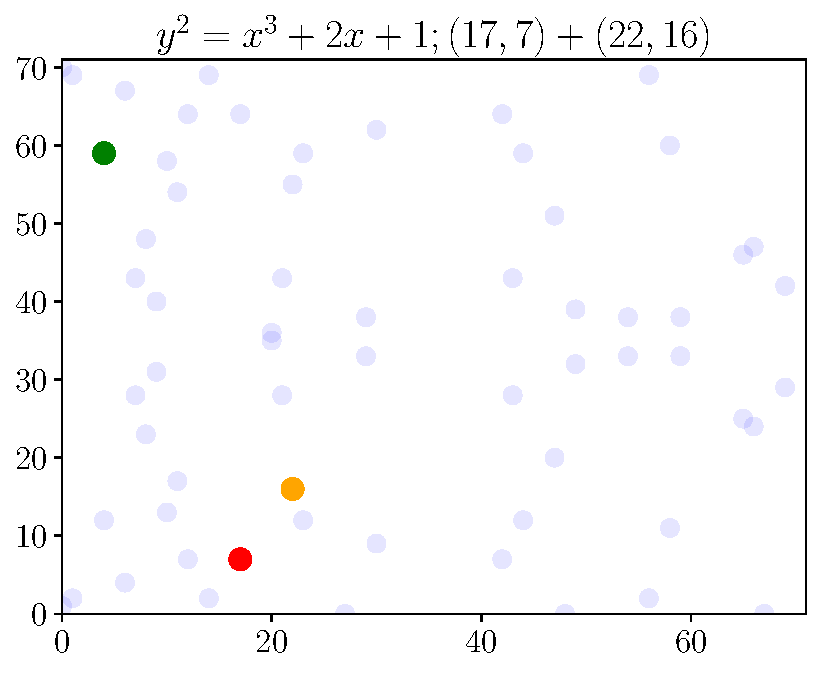
\includegraphics[width=\textwidth]{plots/ec_finite/ec_finite_F_71_2_1_addition_22_16.pdf}
    \caption{$\textcolor{red}{\parens{17,7}}
        + \textcolor{orange}{\parens{22,16}}
        = \textcolor[rgb]{0,0.33,0}{\parens{4,59}}$}
    \end{subfigure}

    \begin{subfigure}[t]{0.45\textwidth}
    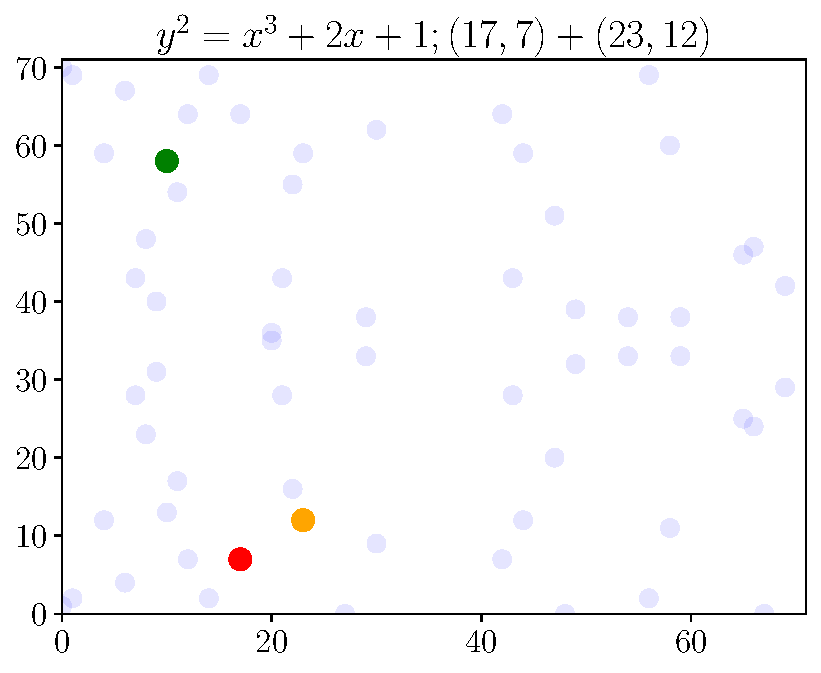
\includegraphics[width=\textwidth]{plots/ec_finite/ec_finite_F_71_2_1_addition_23_12.pdf}
    \caption{$\textcolor{red}{\parens{17,7}}
        + \textcolor{orange}{\parens{23,12}}
        = \textcolor[rgb]{0,0.33,0}{\parens{10,58}}$}
    \end{subfigure}
    \begin{subfigure}[t]{0.45\textwidth}
    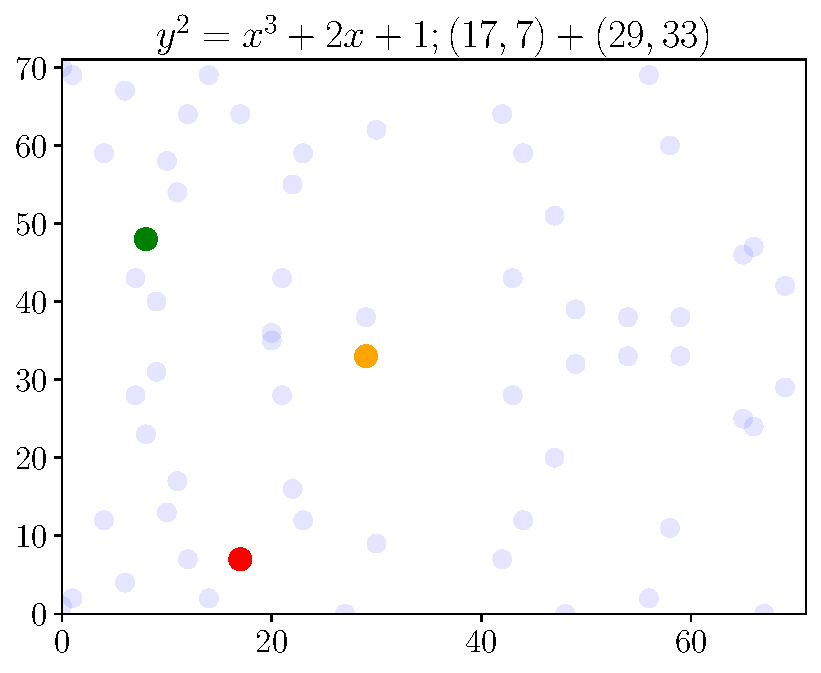
\includegraphics[width=\textwidth]{plots/ec_finite/ec_finite_F_71_2_1_addition_29_33.pdf}
    \caption{$\textcolor{red}{\parens{17,7}}
        + \textcolor{orange}{\parens{29,33}}
        = \textcolor[rgb]{0,0.33,0}{\parens{8,48}}$}
    \end{subfigure}
    \caption[Plots of elliptic curve addition over finite fields]{Here
        have plots of addition on \glspl{elliptic curve} over $\F_{71}$.
        The \glspl{elliptic curve} are all the same: $y^{2} = x^{3} + 2x + 1$.
        The first plot shows the points on the \gls{elliptic curve};
        the other plots show the addition
        $\textcolor{red}{P} + \textcolor{orange}{Q}
            = \textcolor[rgb]{0,0.33,0}{R}$.
        Throughout the plots, $\color{red} P = \parens{17,7}$.
        }
    \label{fig:ec_finite_plots_addition}
\end{figure}

\end{example}


\subsection{Elliptic Curve Scalar Multiplication}
\label{ssec:ec_scalar_mult}

In Chapter~\ref{ssec:ec_subgroups}, we will want to repeatedly add
a point on an \gls{elliptic curve} to itself.
That is, we will want to compute $k\cdot P$ for $k\in\Z$
and $P\in E\parens{\F_{p}}$.
This is defined as

\begin{equation}
    k\cdot P \mathDef{} 
        \underbrace{P + P + \cdots + P}_{\text{$k$ times}}, \quad k\ge 0.
\end{equation}

\noindent
Similarly, we have

\begin{equation}
    k\cdot P \mathDef{} 
        \underbrace{-P - P - \cdots - P}_{\text{$-k$ times}}, \quad k< 0.
\end{equation}

\noindent
This is called \emph{elliptic curve point multiplication} or
\emph{elliptic curve scalar multiplication}.
We remember that if $P\in E(\F_{p})$ and $E$ is in Weierstrass form
with $P = \parens{x,y}$, then $-P = \parens{x,-y}$.
Thus, point negation has negligible cost.

We recall that, in practice, we will define \glspl{elliptic curve} over
$\F_{p}$ with $p$ being a 256-bit prime number.
Thus, $k$ will also be a 256-bit number.
Computing $k\cdot P$ by performing

\begin{align}
    2P &= P + P  \nonumber\\
    3P &= P + 2P \nonumber\\
    4P &= P + 3P \nonumber\\
    5P &= P + 4P \nonumber\\
    &\vdots
\end{align}

\noindent
would take around $2^{256}$ elliptic curve additions.
There is not a fast enough computer to perform the calculation
using this method.

Thankfully, there is a better method called the \emph{double-and-add} method;
see Alg.~\ref{alg:ec_double_and_add} for a formal specification
using \gls{recursion}.
We will walk through the method in Example~\ref{example:ec_double-and-add}.

\begin{algorithm}[t]
\caption{Double-and-add formula for elliptic curve
    scalar multiplication}
\label{alg:ec_double_and_add}
\begin{algorithmic}[1]
\Require $P$ point on \gls{elliptic curve}; $k\in\N$
\Procedure{DoubleAndAdd}{$P$, $k$}
    \If {$k=0$}
        \State \Return $\mathcal{O}$
    \ElsIf {$k=1$}
        \State \Return $P$
    \ElsIf {$k\equiv0\mod 2$}
        \State \Return $\textsc{DoubleAndAdd}(P+P, k/2)$
    \Else
        \State \Return $\textsc{DoubleAndAdd}(P+P, (k-1)/2)+P$
    \EndIf
\EndProcedure
\end{algorithmic}
\end{algorithm}


While this is an efficient algorithm to compute $k\cdot P$,
the branch logic will \emph{leak information} about $k$.
For instance, this type of operation occurs when $k$
could be a private key.
Thus, if this operation is not performed in a secure method
\emph{independent} of $k$, the private key could be
revealed~\cite{cryptoeprint:2014:140}.

We note that the double-and-add formula may be used
when computing large exponentiations as well;
the algorithms are the same except for switching the operations
from doubling and addition to squaring and multiplication.

\begin{example}[Double-and-Add Example]
\label{example:ec_double-and-add}
\exampleCodeReference{examples/math\_review/elliptic\_curve\_double-and-add.py}

We continue using the \gls{elliptic curve}

\begin{equation}
    E: y^{2} = x^{3} + 2x + 1
\end{equation}

\noindent
defined over $\F_{71}$ as before.
We want to compute

\begin{equation}
    29\cdot\parens{0,1}.
\end{equation}

We will use Alg.~\ref{alg:ec_double_and_add}.
We first see that

\begin{equation}
    \parens{0,1} + \parens{0,1} = \parens{1,69}.
\end{equation}

\noindent
We have

\begin{equation}
    \textsc{DoubleAndAdd}\brackets{\parens{0,1}, 29}
    = \parens{0,1} + \textsc{DoubleAndAdd}\brackets{\parens{1,69}, 14}.
\end{equation}

\noindent
Next, we see

\begin{equation}
    \parens{1,69} + \parens{1,69} = \parens{4,59}.
\end{equation}

\noindent
We then compute

\begin{equation}
    \textsc{DoubleAndAdd}\brackets{\parens{1,69}, 14}
    = \textsc{DoubleAndAdd}\brackets{\parens{4,59}, 7}.
\end{equation}

\noindent
In the next step, we find

\begin{equation}
    \parens{4,59} + \parens{4,59} = \parens{56,2}.
\end{equation}

\noindent
After this, we have

\begin{equation}
    \textsc{DoubleAndAdd}\brackets{\parens{4,59}, 7}
    = \parens{4,59} + \textsc{DoubleAndAdd}\brackets{\parens{56,2}, 3}.
\end{equation}

\noindent
Another addition gives us

\begin{equation}
    \parens{56,2} + \parens{56,2} = \parens{67,0}.
\end{equation}

\noindent
The final iteration gives us

\begin{align}
    \textsc{DoubleAndAdd}\brackets{\parens{56,2}, 3}
        &= \parens{56,2} + \textsc{DoubleAndAdd}\brackets{\parens{67,0}, 1}
            \nonumber\\
    &= \parens{56,2} + \parens{67,0}.
\end{align}

\noindent
Our algorithm has stopped.

At this point, we can add all of the points we have computed.
Doing this, we see

\begin{align}
    29\cdot\parens{0,1} &=
            \parens{0,1} + \braces{\parens{4,59} + \brackets{
                \parens{56,2} + \parens{67,0}}}
        \nonumber\\
    &= \parens{0,1} + \braces{\parens{4,59} + \parens{56,69}}
        \nonumber\\
    &= \parens{0,1} + \parens{4,12}
        \nonumber\\
    &= \parens{8,48}.
\end{align}

\noindent
This took us 7 additions on the \gls{elliptic curve};
this is much less than 29.
\end{example}

In fact, using Alg.~\ref{alg:ec_double_and_add},
the computation is logarithmic in $k$;
that is, it will take $O(\log(k)^{c})$ steps for small constant $c>0$.


\subsection{Subgroups of Elliptic Curves over Finite Fields}
\label{ssec:ec_subgroups}

We now have the addition formula
and the ability to efficiently add points.
\emph{This} allows us to create \glspl{subgroup} of \glspl{elliptic curve}
over \glspl{finite field} for \gls{ecc}.

We let $P\in E(\F_{p})$ be a point on an \gls{elliptic curve}.
We define the following \gls{subgroup}:

\begin{equation}
    \angles{P} \mathDef{} \braces{k\cdot P \mid k\in\Z}.
\end{equation}

\noindent
Naturally, we have $\angles{P}\le E(\F_{p})$;
more explicitly, $\angles{P}$ is the \gls{subgroup}
of the \gls{elliptic curve} $E(\F_{p})$
formed by looking at all the points on the \gls{elliptic curve}
which we can get by adding $P$ to itself.
We can always look at \glspl{subgroup} of this form over general
\glspl{elliptic curve};
when we restrict our attention to \glspl{finite field},
then the \glspl{elliptic curve} are \glspl{finite group}.
These \glspl{finite group} allow us to look at the
\emph{\gls{dlp}}:
If $Q \in \angles{P}$, determine $x\in\Z$ such that

\begin{equation}
    Q = x\cdot P.
\end{equation}

\noindent
For many \glspl{elliptic curve}, this is difficult problem.
This is discussed more in Chapter~\ref{chap:hardness}.

See Figure~\ref{fig:ec_finite_plots_subgroups}
for example cyclic subgroups of \glspl{elliptic curve} over
\glspl{finite field}.

\begin{figure}[p]
\centering
    \begin{subfigure}[t]{0.45\textwidth}
    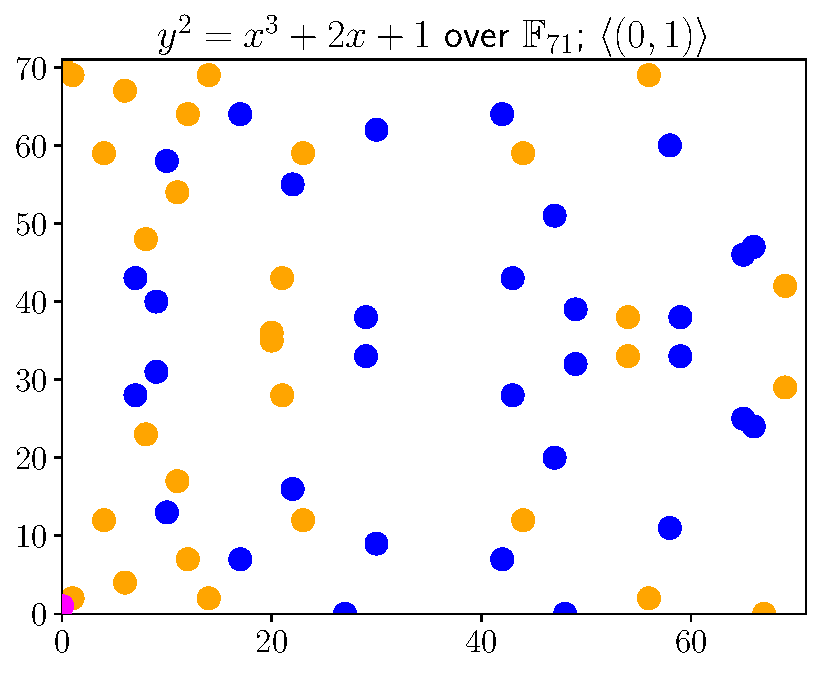
\includegraphics[width=\textwidth]{plots/ec_finite/ec_finite_F_71_2_1_subgroup_0_1.pdf}
    \caption{\textcolor{orange}{Subgroup} generated by
        $\color{magenta} \parens{0,1}$}
    \label{fig:ec_finite_plots_subgroups_0_1}
    \end{subfigure}
    \begin{subfigure}[t]{0.45\textwidth}
    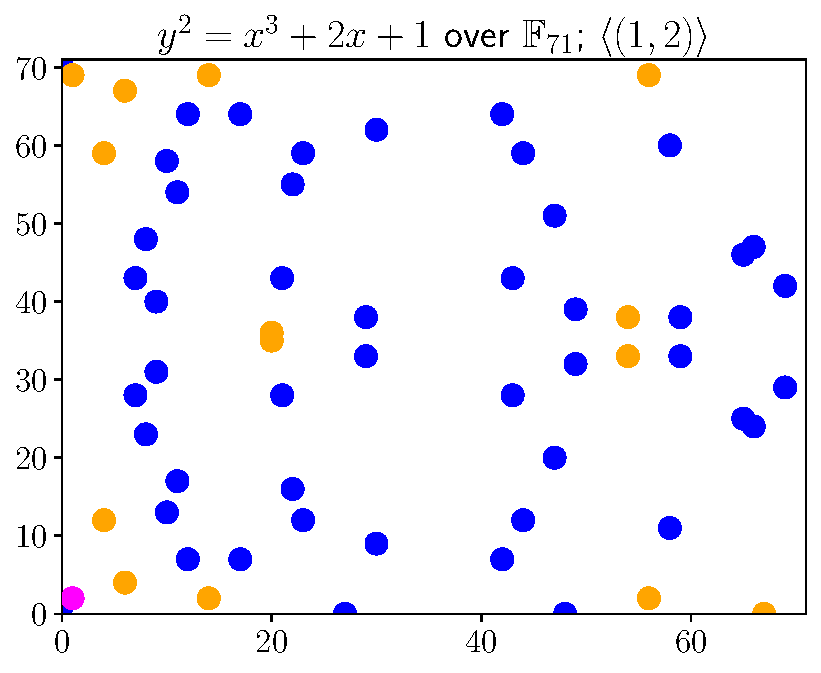
\includegraphics[width=\textwidth]{plots/ec_finite/ec_finite_F_71_2_1_subgroup_1_2.pdf}
    \caption{\textcolor{orange}{Subgroup} generated by
        $\color{magenta}\parens{1,2}$}
    \label{fig:ec_finite_plots_subgroups_1_2}
    \end{subfigure}

    \begin{subfigure}[t]{0.45\textwidth}
    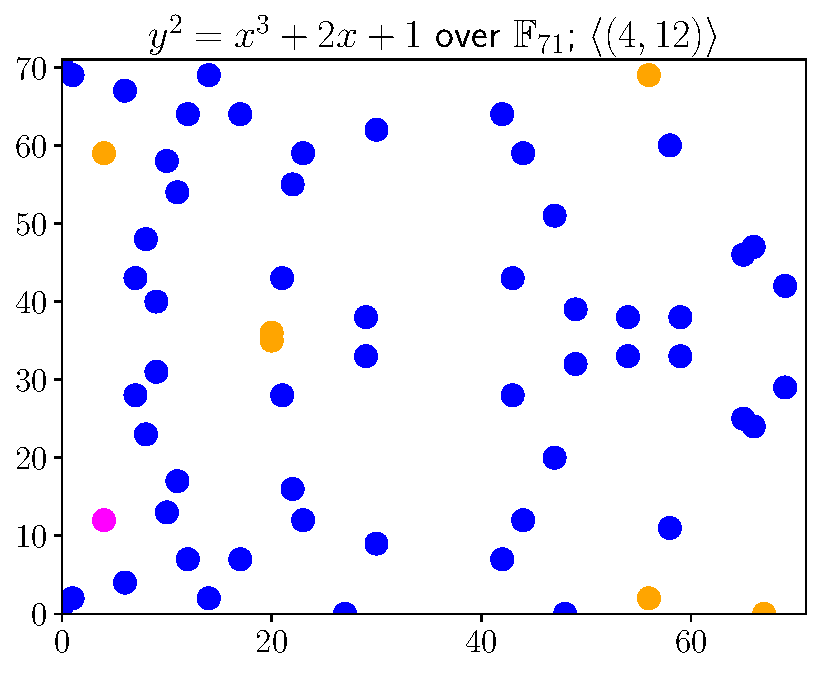
\includegraphics[width=\textwidth]{plots/ec_finite/ec_finite_F_71_2_1_subgroup_4_12.pdf}
    \caption{\textcolor{orange}{Subgroup} generated by
        $\color{magenta}\parens{4,12}$}
    \label{fig:ec_finite_plots_subgroups_4_12}
    \end{subfigure}
    \begin{subfigure}[t]{0.45\textwidth}
    \includegraphics[width=\textwidth]{plots/ec_finite/ec_finite_F_71_2_1_subgroup_6_4.pdf}
    \caption{\textcolor{orange}{Subgroup} generated by
        $\color{magenta}\parens{6,4}$}
    \label{fig:ec_finite_plots_subgroups_6_4}
    \end{subfigure}

    \begin{subfigure}[t]{0.45\textwidth}
    \includegraphics[width=\textwidth]{plots/ec_finite/ec_finite_F_71_2_1_subgroup_7_28.pdf}
    \caption{\textcolor{orange}{Subgroup} generated by
        $\color{magenta}\parens{7,28}$}
    \label{fig:ec_finite_plots_subgroups_7_28}
    \end{subfigure}
    \begin{subfigure}[t]{0.45\textwidth}
    \includegraphics[width=\textwidth]{plots/ec_finite/ec_finite_F_71_2_1_subgroup_10_13.pdf}
    \caption{\textcolor{orange}{Subgroup} generated by
        $\color{magenta}\parens{10,13}$}
    \label{fig:ec_finite_plots_subgroups_10_13}
    \end{subfigure}
    \caption[Plots of subgroups of elliptic curves over finite fields]{Here
        are plots of \glspl{elliptic curve} over $\F_{71}$.
        The \glspl{elliptic curve} are all the same: $y^{2} = x^{3} + 2x + 1$.
        In each plot, we also show different cyclic subgroups;
        \textcolor{orange}{subgroups} generated by different
        \textcolor{magenta}{base points}.}
    \label{fig:ec_finite_plots_subgroups}
\end{figure}


\begin{example}[Subgroups of Elliptic Curves]
\exampleCodeReference{examples/math\_review/elliptic\_curve\_subgroup.py}

In this example we look at \glspl{subgroup} on an \gls{elliptic curve}.
We will focus on the \gls{elliptic curve}

\begin{equation}
    E: y^{2} = x^{3} + 2x + 1
\end{equation}

\noindent
over $\F_{71}$.
Plots of various \glspl{subgroup} are found in
Figure~\ref{fig:ec_finite_plots_subgroups}.

We will focus on $\angles{\parens{1,2}}$;
this can be seen in
Figure~\ref{fig:ec_finite_plots_subgroups_1_2}.
If we list out all the points of the \gls{subgroup}, we see

\begin{align}
    1\cdot \parens{1,2}  &= \parens{1,2}
        &
    9\cdot \parens{1,2}  &= \parens{6,67} \nonumber\\
    2\cdot \parens{1,2}  &= \parens{4,12}
        &
    10\cdot \parens{1,2} &= \parens{20,35} \nonumber\\
    3\cdot \parens{1,2}  &= \parens{14,2}
        &
    11\cdot \parens{1,2} &= \parens{54,33} \nonumber\\
    4\cdot \parens{1,2}  &= \parens{56,69}
        &
    12\cdot \parens{1,2} &= \parens{56,2} \nonumber\\
    5\cdot \parens{1,2}  &= \parens{54,38}
        &
    13\cdot \parens{1,2} &= \parens{14,69} \nonumber\\
    6\cdot \parens{1,2}  &= \parens{20,36}
        &
    14\cdot \parens{1,2} &= \parens{4,59} \nonumber\\
    7\cdot \parens{1,2}  &= \parens{6,4}
        &
    15\cdot \parens{1,2} &= \parens{1,69} \nonumber\\
    8\cdot \parens{1,2}  &= \parens{67,0}
        &
    16\cdot \parens{1,2} &= \mathcal{O}.
    \label{eq:elliptic_ecdlp}
\end{align}

\noindent
As we look at the point distribution and compare it with
the rest of the points,
there does not appear to be any structure between
the points in the \gls{subgroup} or not.
It is this apparent lack of structure that makes \gls{elliptic curve}
\glspl{group} great for \gls{publiccrypto}.

We note that the \glspl{subgroup} in
Figures~\ref{fig:ec_finite_plots_subgroups_1_2}
and \ref{fig:ec_finite_plots_subgroups_6_4} are the same;
this means that the points $\parens{1,2}$ and $\parens{6,4}$
generate the same \glspl{subgroup}.
\end{example}

\begin{example}[Elliptic Curve Discrete Logarithm]
We continue the previous example with the same \gls{elliptic curve}
and \gls{subgroup}.

We want to find $x$ such that

\begin{equation}
    x\cdot\parens{1,2} = \parens{54,33}.
\end{equation}

\noindent
Because the addition formula for points on \glspl{elliptic curve} is ``random'',
there does not appear to be any better way to find
$x$ than to just list out every possibility.
From looking at all the scalar multiplications
in Eq.~\eqref{eq:elliptic_ecdlp},
we see that $x = 11$.
\end{example}

We note that generic methods for solving the \gls{elliptic curve} \gls{dlp}
are discussed in Chapter~\ref{sec:hardness_dlp}.


\subsection{Elliptic Curve Point Compression}
\label{ssec:ec_point_compression}

Due to the fact that \glspl{elliptic curve} satisfy an algebraic equation,
we are able to \emph{compress} points on the \gls{elliptic curve}
so that they take up less space.

We assume that $p$ is an odd prime.
As before, let us look at an \gls{elliptic curve} $E/\F_{p}$
and suppose that we have a point on the \gls{elliptic curve}
$P = \parens{x,y}$.
We know that we have the relation

\begin{equation}
    y^{2} = x^{3} + ax + b.
\end{equation}

\noindent
for some specified $a,b\in\F_{p}$.

If we only knew $x$, then we can solve for $y$:

\begin{equation}
    y = \pm\sqrt{x^{3} + ax + b}.
\end{equation}

\noindent
The challenge is to then determine \emph{which} $y$ value
is the appropriate one.
We see that such a square root must exist, so we set

\begin{equation}
    s \mathDef{} \sqrt{x^{3} + ax + b}.
    \label{eq:ec_compress_sqrt}
\end{equation}

\noindent
Note well that this square root is a \emph{modular square root},
not a regular square root.
Thus, we have

\begin{equation}
    y = \pm s.
\end{equation}

Now, we remember that all of these operations are modular arithmetic
operations modulo a prime $p$.
Thus, we know $s\in\braces{0, 1, 2, \cdots, p-1}$.
We also remember that

\begin{equation}
    -s = p - s \mod p.
\end{equation}

\noindent
Because we are assuming that $p$ is an odd prime,
we know there are two possibilities:
$s$ is even and $p-s$ is odd; or
$s$ is odd and $p-s$ is even.

We can use these facts to compress the point $P = \parens{x,y}$
on an \gls{elliptic curve};
this allows for more efficient transmission.
For instance, suppose that $p$ is an $n$-bit prime.
In this case, the uncompressed form of representing $P$
requires $2n$ bits.
The compressed form only requires $n+1$ bits: $n$ bits to store $x$
and $1$ bit to store whether $y$ is even or odd.
By using the compressed form, storage is essentially halved.
This assumes that the particular \gls{elliptic curve} being used
is public knowledge so that $a$ and $b$ are known.

We did not mention \emph{how} to compute $s$ in
Eq.~\eqref{eq:ec_compress_sqrt}.
Methods for computing square roots in \glspl{finite field}
may be found in Appendix~\ref{app:math_finite_fields}.

\begin{example}[Elliptic Curve Point Compression]
\exampleCodeReference{examples/math\_review/elliptic\_curve\_compression.py}

We continue to work with the \gls{elliptic curve}

\begin{equation}
    E: y^{2} = x^{3} + 2x + 1
\end{equation}

\noindent
over $\F_{71}$.

If we want to compress the point $\parens{17,7}$,
then we need to send $\parens{17,\texttt{0b1}}$;
we send \texttt{0b1} because the $y$-coordinate $7$ is odd.

Suppose we receive the compressed point $\parens{47,\texttt{0b0}}$.
Thus, the $x$-coordinate is $47$ and the $y$-coordinate is even.
We see that

\begin{align}
    t &\mathDef{} x^{3} + ax + b \mod p\nonumber\\
        &= 47^{3} + 2\cdot47 + 1 \mod 71 \nonumber\\
        &= 45.
\end{align}

\noindent
We can verify that

\begin{equation}
    51^{2} \mod 71 = 45.
\end{equation}

\noindent
Thus, $51$ is a square root of $45$.
It follows that

\begin{align}
    s &\mathDef{} \sqrt{t} \mod p \nonumber\\
        &= 51.
\end{align}

\noindent
We note, though, that $s$ is odd although we were told $y$ is even;
thus, we have

\begin{align}
    y &\mathDef{} p - s \nonumber\\
        &= 20.
\end{align}

\noindent
Therefore, the point in uncompressed form is

\begin{equation}
    P = \parens{47,20}.
\end{equation}
\end{example}

As we can see from the above example,
the point compression for \glspl{elliptic curve} trades
storage for computation.
Compression may be worthwhile in situations where
storage is relatively expensive.

\subsection{Examples of Specific Curves}
\label{ssec:specific_curves}

We now include some specific curves used in practice.
We also bring them up because some of them have forms different
than the Weierstrass form we have been using.

While it is very easy to come up with additional \glspl{elliptic curve},
developing new \glspl{elliptic curve} for cryptography requires
\emph{extreme care}.
Doing this is \emph{highly discouraged}, as it amounts to
``rolling your own crypto''.
This was frowned upon in Chapter~\ref{chap:do_not}.

Whenever possible, use a well-tested library developed by
experienced cryptologists.
If this is not possible, \emph{proceed with caution}.

\subsubsection{Secp256k1}

This \gls{elliptic curve} is used by both Bitcoin~\cite{BitcoinWhitepaper} and
\gls{ethereum}~\cite[Appendix F]{EthereumYellowpaper}
for \glspl{signature}.
It has the form

\begin{equation}
    E:y^{2} = x^{3} + 7
\end{equation}

\noindent
over the \gls{field} $\F_{q}$ with

\begin{equation}
    q = 2^{256} - 2^{32} - 2^{9} - 2^{8} - 2^{7} - 2^{6} - 2^{4} - 1.
\end{equation}

\noindent
It was defined in~\cite[Section 2.4.1]{brown2010sec2}.

\subsubsection{Curve25519}

This curve~\cite{Curve25519} is used in X25519,
the \gls{dhke} based on this curve.
We have

\begin{equation}
    E:y^{2} = x^{3} + 486662x^{2} + x
\end{equation}

\noindent
over the prime \gls{field} $\F_{q}$,
where

\begin{equation}
    q = 2^{255} - 19.
\end{equation}

\noindent
This is a \emph{Montgomery curve}.
A general Montgomery curve has the form

\begin{equation}
    M_{A,B}: By^{2} = x^{3} + Ax^{2} + x
\end{equation}

\noindent
over a field $K$ with $A,B\in K$.
Having this specific form allows for some operations to be
efficiently computed.

\subsubsection{Ed25519}

This is one of the \glspl{elliptic curve} used for the
Edwards Curve Digital Signature Algorithm (EdDSA)~\cite{ed25519}.
It is birationally equivalent to Curve25519~\cite{Curve25519}.
We have

\begin{equation}
    E:-x^{2} + y^{2} = 1 - \frac{121665}{121666}x^{2}y^{2}
\end{equation}

\noindent
over the \gls{field} $\F_{q}$ with

\begin{equation}
    q = 2^{255}-19.
\end{equation}

\noindent
This is a \emph{twisted Edwards curve}.
In general, a twisted Edwards curve has the form

\begin{equation}
    E_{E,a,d}:ax^{2} + y^{2} = 1 + dx^{2}y^{2}
\end{equation}

\noindent
over a field $K$ with $a,d\in K$ distinct.
There is a minor technical restriction on the field $K$
which we do not mention.

\subsection{Encoding Elliptic Curves over Finite Fields}

When working with the \glspl{elliptic curve} $E/\F_{p}$,
we can encode $\parens{x,y}$ using its binary representation;
encoding the identity element $\mathcal{O}$ may require care.
It may be useful to use point compression described
in Chapter~\ref{ssec:ec_point_compression} depending on the situation.

\section{Bilinear Pairings}
\label{sec:math_pairings}

\subsection{Why do we care about Bilinear Pairings?}

We care about \glspl{bilinear} because they give us a lot of nice
mathematical features that we can use.
In particular, \glspl{bilinear} give us
\emph{short digital signatures}.
These started with BLS signatures based on the Weil
pairing~\cite{BLSSignatures},
a particular type of \gls{bilinear}.

\Glspl{bilinear} also allow for threshold group signatures.
These can be formed as part of a \gls{distributed key generation}
protocol and are discussed in Chapter~\ref{chap:secret_sharing}.

\subsection{Formal Definition}

A \gls{bilinear} is a special type of \gls{function}:

\begin{defn}[Bilinear Pairing]
We let $G_{1}$, $G_{2}$, and $G_{T}$ be \glspl{finite group} with
$\abs{G_{1}} = \abs{G_{2}} = \abs{G_{T}}$.
We say $e:G_{1}\times G_{2}\to G_{T}$ is a \emph{\gls{bilinear}}
if for all $h_{1}\in G_{1}$, $h_{2}\in G_{2}$, and $a,b\in\Z$
we have

\begin{equation}
    e\parens{h_{1}^{a},h_{2}^{b}} = \brackets{e\parens{h_{1},h_{2}}}^{ab}.
\end{equation}
\end{defn}

\subsection{Discussion}

It is straightforward to \emph{use} the previous definition.
The challenge is \emph{finding} \glspl{group} with which to build such a
\gls{bilinear}.
This is nontrivial.

At this point, all \glspl{bilinear} arise from \glspl{elliptic curve}.
The exact construction is complex and we do not discuss it here.
We will use \glspl{bilinear} in Chapter~\ref{chap:pairing}
when we discuss \gls{pairingcrypto}.
Having a solid understanding of the mathematics behind pairings
and how they are constructed from \glspl{elliptic curve}
requires advanced knowledge of \glspl{elliptic curve} as discussed
in~\cite{AEC}.

\section{Lagrange Interpolation}
\label{sec:math_lagrange}

We spend some time discussing \gls{lagrange interpolation}.

\subsection{Why do we care about interpolation?}

Within cryptography, \emph{\gls{lagrange interpolation}}
over \glspl{finite field}
is used in secret sharing protocols and \gls{distributed key generation}.
More generally, interpolation is useful because
it attempts to approximate a complex function with a simpler polynomial.

We will start by looking at interpolation over real data.
After working through examples, we will transition
to interpolation over \glspl{finite field} as this is our primary focus.

\subsection{Lagrange Interpolation over the Reals}

Given a set of data points $\braces{\parens{x_{k},y_{k}}}_{k=1}^{n}$
with $\braces{x_{k}}_{k=1}^{n}$ distinct,
we want to find the interpolating polynomial of minimal degree
which agrees with the data.
That is, we want a polynomial $p$ of at most degree $n-1$ such that

\begin{equation}
    p(x_{k}) = y_{k}, \quad k\in\braces{1,\cdots,n}.
\end{equation}

We now proceed to construct such a polynomial.
To do this, we set

\begin{align}
    L(x) &\mathDef{} \sum_{k=1}^{n} y_{k}\ell_{k}(x) \nonumber\\
    \ell_{k}(x) &\mathDef{}
        \prod_{\substack{1\le j \le n \\ j\ne k}} \frac{x-x_{j}}{x_{k}-x_{j}}
            \nonumber\\
        &=
        \frac{x-x_{1}}{x_{k}-x_{1}}\cdot
        \frac{x-x_{2}}{x_{k}-x_{2}}\cdots
        \frac{x-x_{k-1}}{x_{k}-x_{k-1}}\cdot
        \frac{x-x_{k+1}}{x_{k}-x_{k+1}}\cdots
        \frac{x-x_{n}}{x_{k}-x_{n}}.
    \label{eq:math_lagrange_def}
\end{align}

\noindent
We note that $\ell_{k}$ is a polynomial of degree $n-1$;
this implies that $L$ is a polynomial of degree at most $n-1$.
We note that

\begin{align}
    \ell_{k}(x_{j}) &=
        \begin{cases} 1, \quad k = j \\ 0, \quad k\ne j \end{cases}
            \nonumber\\
        &= \del_{kj}.
\end{align}

\noindent
Here, $\del_{kj}$ is the Kronecker delta.
It follows that 

\begin{align}
    L(x_{j}) &= \sum_{k=1}^{n}y_{k}\ell_{k}(x_{j}) \nonumber\\
        &= \sum_{k=1}^{n} y_{k}\del_{kj} \nonumber\\
        &= y_{j}.
\end{align}

\noindent
Thus, this is the interpolating polynomial which agrees
with the data.
Furthermore, the degree of the polynomial is at most $n-1$.
Such polynomials are unique.

\subsection{Examples of Lagrange Interpolation over the Reals}

\begin{example}
\label{example:math_lagrange_reals_1}
\exampleCodeReference{examples/math\_review/lagrange\_reals\_1.py}

We begin by interpolating the data
$\braces{\parens{1,2},\parens{4,1},\parens{7,8}}$.
See the data in Figure~\ref{fig:lagrange_points_1}.

\begin{figure}[t]
\centering
    \begin{subfigure}[t]{0.45\textwidth}
    \includegraphics[width=\textwidth]{plots/lagrange/lagrange_reals_points_1.pdf}
    \caption{Lagrange interpolation data points}
    \label{fig:lagrange_points_1}
    \end{subfigure}
    \begin{subfigure}[t]{0.45\textwidth}
    \includegraphics[width=\textwidth]{plots/lagrange/lagrange_reals_poly_1.pdf}
    \caption{Lagrange interpolation polynomial}
    \label{fig:lagrange_poly_1}
    \end{subfigure}
    \caption[Data points and Lagrange Interpolation over the reals 1]{Here
        are data points and Lagrange interpolating polynomial
        for Example~\ref{example:math_lagrange_reals_1}.}
\end{figure}



We start by computing the $\ell_{k}$ polynomials:

\begin{align}
    \ell_{1}(x) &= \frac{x-4}{1-4}\cdot\frac{x-7}{1-7}
        \nonumber\\
    \ell_{2}(x) &= \frac{x-1}{4-1}\cdot\frac{x-7}{4-7}
        \nonumber\\
    \ell_{3}(x) &= \frac{x-1}{7-1}\cdot\frac{x-4}{7-4}.
\end{align}

\noindent
In this case, we have the interpolating polynomial

\begin{equation}
    L(x) = 2\cdot\frac{x-4}{1-4}\cdot\frac{x-7}{1-7}
        + 1\cdot\frac{x-1}{4-1}\cdot\frac{x-7}{4-7}
        + 8\cdot\frac{x-1}{7-1}\cdot\frac{x-4}{7-4}.
\end{equation}

\noindent
This may be reduced to

\begin{equation}
    L(x) = \frac{1}{9}\brackets{4x^{2} - 23x + 37}.
\end{equation}

\noindent
The data points with this polynomial can be found in
Figure~\ref{fig:lagrange_poly_1}.
We see that

\begin{align}
    L(1) &= 2 \nonumber\\
    L(4) &= 1 \nonumber\\
    L(7) &= 8.
\end{align}
\end{example}

\begin{example}
\label{example:math_lagrange_reals_2}
\exampleCodeReference{examples/math\_review/lagrange\_reals\_2.py}

We interpolate the data
$\braces{\parens{1,2},\parens{4,1},\parens{5,1},\parens{7,8}}$;
this is the same data from the previous example with the additional
point $\parens{5,1}$.
See the data in Figure~\ref{fig:lagrange_points_2}.

\begin{figure}[t]
\centering
    \begin{subfigure}[t]{0.45\textwidth}
    \includegraphics[width=\textwidth]{plots/lagrange/lagrange_reals_points_2.pdf}
    \caption{Lagrange interpolation data points}
    \label{fig:lagrange_points_2}
    \end{subfigure}
    \begin{subfigure}[t]{0.45\textwidth}
    \includegraphics[width=\textwidth]{plots/lagrange/lagrange_reals_poly_2.pdf}
    \caption{Lagrange interpolation polynomial}
    \label{fig:lagrange_poly_2}
    \end{subfigure}
    \caption[Data points and Lagrange Interpolation over the reals 2]{Here
        are data points and Lagrange interpolating polynomial
        for Example~\ref{example:math_lagrange_reals_2}.}
\end{figure}



We again compute the $\ell_{k}$ polynomials:

\begin{align}
    \ell_{1}(x) &= \frac{x-4}{1-4}\cdot\frac{x-5}{1-5}\cdot\frac{x-7}{1-7}
        \nonumber\\
    \ell_{2}(x) &= \frac{x-1}{4-1}\cdot\frac{x-5}{4-5}\cdot\frac{x-7}{4-7}
        \nonumber\\
    \ell_{3}(x) &= \frac{x-1}{5-1}\cdot\frac{x-4}{5-4}\cdot\frac{x-7}{5-7}
        \nonumber\\
    \ell_{4}(x) &= \frac{x-1}{7-1}\cdot\frac{x-4}{7-4}\cdot\frac{x-5}{7-5}.
\end{align}

\noindent
The resulting Lagrange interpolation polynomial is

\begin{equation}
    L(x) = \frac{1}{72}\brackets{13x^{3} - 124x^{2} + 323x - 68}.
\end{equation}

\noindent
The data points with this polynomial can be found in
Figure~\ref{fig:lagrange_poly_2}.
\end{example}

\subsection{Problems with Lagrange Interpolation over the Reals}

We note that using \gls{lagrange interpolation} can lead to problems
when attempting to approximate certain types of \glspl{function} (data).
In particular, even with smooth functions
(functions with infinitely many derivatives),
it is possible that the polynomial approximation given by
\gls{lagrange interpolation} does not converge to the underlying function.
An example of this is shown in Figure~\ref{fig:math_lagrange_runge};
this is called \emph{Runge's Phenomenon}.

\begin{figure}[t]
\centering
    \includegraphics[width=10cm]{plots/lagrange/lagrange_runge.pdf}
    \caption[Plot of Runge's Phenomenon]{Here
        is an example of Runge's phenomenon.
        Even though the polynomial approximation of the \gls{function}
        $f(x) = \brackets{1+25x^{2}}^{-1}$
        is accurate close to $0$, the approximation is very poor
        near $1$ and $-1$.}
    \label{fig:math_lagrange_runge}
\end{figure}


There are mathematical reasons which can explain this,
but \emph{none} of those difficulties matter to us
because we are not particularly interested in interpolating
\glspl{function} over $\R$.
Rather, we are interested in interpolating polynomials over
\glspl{finite field}.

\subsection{Lagrange Interpolation over Finite Fields}

We are particularly interested in performing \gls{lagrange interpolation}
over \glspl{finite field}.
This will be used in secret sharing protocols.

There is effectively no difference between interpolation
over $\R$ and interpolation over $\F_{p}$.
This is because all of the operations in $\R$ directly translate
into the equivalent operations in $\F_{p}$.

\subsection{Examples of Lagrange Interpolation over Finite Fields}

We use the same examples as before except that now we use
the \gls{finite field} $\F_{73}$.



\begin{example}
\label{example:math_lagrange_finite_1}
\exampleCodeReference{examples/math\_review/lagrange\_finite\_1.py}

We begin by interpolating the data
$\braces{\parens{1,2},\parens{4,1},\parens{7,8}}$ as before
in Example~\ref{example:math_lagrange_reals_1};
in this case, we are interpolating over $\F_{73}$.
See the data in Figure~\ref{fig:lagrange_finite_points_1}.

\begin{figure}[t]
\centering
    \begin{subfigure}[t]{0.45\textwidth}
    \includegraphics[width=\textwidth]{plots/lagrange/lagrange_finite_points_1.pdf}
    \caption{Lagrange interpolation data points}
    \label{fig:lagrange_finite_points_1}
    \end{subfigure}
    \begin{subfigure}[t]{0.45\textwidth}
    \includegraphics[width=\textwidth]{plots/lagrange/lagrange_finite_poly_1.pdf}
    \caption{Lagrange interpolation polynomial}
    \label{fig:lagrange_finite_poly_1}
    \end{subfigure}
    \caption[Data points and Lagrange Interpolation over finite fields 1]{Here
        are data points and Lagrange interpolating polynomial
        for Example~\ref{example:math_lagrange_finite_1}.
        This example uses the \gls{finite field} $\F_{73}$.}
\end{figure}



In this case, we have the interpolating polynomial

\begin{equation}
    L(x) = 41x^{2} + 38x + 69.
\end{equation}

\noindent
The data points with this polynomial can be found in
Figure~\ref{fig:lagrange_finite_poly_1}.
We see that

\begin{align}
    L(1) &= 2 \nonumber\\
    L(4) &= 1 \nonumber\\
    L(7) &= 8.
\end{align}
\end{example}

\begin{example}
\label{example:math_lagrange_finite_2}
\exampleCodeReference{examples/math\_review/lagrange\_finite\_2.py}

We interpolate the data
$\braces{\parens{1,2},\parens{4,1},\parens{5,1},\parens{7,8}}$ as
in Example~\ref{example:math_lagrange_reals_2};
in this case, we are interpolating over $\F_{73}$.
See the data in Figure~\ref{fig:lagrange_finite_points_2}.

\begin{figure}[t]
\centering
    \begin{subfigure}[t]{0.45\textwidth}
    \includegraphics[width=\textwidth]{plots/lagrange/lagrange_finite_points_2.pdf}
    \caption{Lagrange interpolation data points}
    \label{fig:lagrange_finite_points_2}
    \end{subfigure}
    \begin{subfigure}[t]{0.45\textwidth}
    \includegraphics[width=\textwidth]{plots/lagrange/lagrange_finite_poly_2.pdf}
    \caption{Lagrange interpolation polynomial}
    \label{fig:lagrange_finite_poly_2}
    \end{subfigure}
    \caption[Data points and Lagrange Interpolation over finite fields 2]{Here
        are data points and Lagrange interpolating polynomial
        for Example~\ref{example:math_lagrange_finite_2}.
        This example uses the \gls{finite field} $\F_{73}$.}
\end{figure}



In this case, we have the interpolating polynomial

\begin{equation}
    L(x) = 60x^{3} + 51x^{2} + 42x + 68.
\end{equation}

\noindent
The data points with this polynomial can be found in
Figure~\ref{fig:lagrange_finite_poly_2}.
We see that

\begin{align}
    L(1) &= 2 \nonumber\\
    L(4) &= 1 \nonumber\\
    L(5) &= 1 \nonumber\\
    L(7) &= 8.
\end{align}
\end{example}

\subsection{Further Generalizations of Lagrange Interpolation}

It is possible to generalize \gls{lagrange interpolation} more.
In particular, by looking at Eq.~\eqref{eq:math_lagrange_def},
we see that all that is required of the data
$\braces{\parens{x_{i},y_{i}}}_{i=1}^{n}$
is that $\braces{x_{i}}$ must be elements of a \gls{field} $\F$
and $\braces{y_{i}}$ must be elements where it makes sense to perform
multiplication by $\F$.
Although this may appear to be an unnecessary generalization,
this will be used when computing threshold digital signatures
in Chapter~\ref{sec:ss_threshold};
in that setting, we are essentially interpolating over \gls{group} elements
parameterized by elements in a \gls{finite field}.


\section{Conclusion of Mathematical Review}

A lot of important and difficult material was covered
in the previous chapters.
There is still more mathematics that could be learned
and that would be useful for cryptography.
With that said, these are the main ideas and the most useful.
Studying additional mathematics would be recommended to anyone
who wants to dive deeper into cryptography;
see Chapter~\ref{chap:conclusion} for additional resources.

\chapter{Symmetric Key Cryptography}
\label{chap:symmetric}

We now begin our discussion of \gls{symmetriccrypto},
which involves one secret key.
This distinguishes it from \gls{publiccrypto}, which we will
discuss in Chapter~\ref{chap:public}, which uses \emph{two} keys:
one public key and one private key.



\section{The Need for Symmetric Key Cryptography}

Alice and Bob would like to communicate with each other
over an \gls{insecure channel}.
In particular, they know that eavesdropper Eve will frequently
be intercepting their communication,
and they do not want her to be find out what they are saying.

Throughout \gls{symmetriccrypto}, we assume that Alice and Bob
have a shared secret key that they can use for communication.
This secret key has been shared through a \gls{secure channel};
in particular, Eve does \emph{not} know what the key is,
although she does know everything about the \gls{encryption scheme}
they are using.
This ensures that Alice and Bob follow
\emph{Kerchoff's principle}~\cite[Page 5]{IntroModernCrypto}:

\begin{quote}
    The cipher method must not be required to be secret,
    and it must be able to fall into the hands of the enemy
    without inconvenience.
\end{quote}

\noindent
The messages that Alice and Bob send to each other shall be called
the \emph{plaintext}.
When the plaintext has been encrypted, the resulting encrypted message
shall be called the \emph{ciphertext} (also spelled \emph{cyphertext}).



\section{Unbreakable Encryption: the One-Time Pad}

\subsection{Definition}

Suppose Alice has a message $m\in\braces{0,1}^{L}$ to send Bob
and wants to encrypt $m$.
Further suppose that Alice previously shared a secret key
$s\chooseRandom{}\braces{0,1}^{L}$ with Bob.
Here, the key $s$ is a uniformly random bit string.
To encrypt $m$ using the \gls{otp}, the ciphertext $c$ is

\begin{equation}
    c \mathDef{} s \oplus m,
\end{equation}

\noindent
where $\oplus$ is the XOR operation.
She then sends the ciphertext $c$ to Bob over an \gls{insecure channel}
(like the Internet).
Because Bob also knows the secret key $s$,
he is able to recover the message $m$ by the XOR operation:

\begin{align}
    s \oplus c &= s \oplus \parens{s \oplus m} \nonumber\\
        &= m.
\end{align}

\subsection{Examples}

We now look at some examples of encryption using the \gls{otp}.

\begin{example}[One-Time Pad 1]
\exampleCodeReference{examples/symmetric/one-time\_pad\_1.py}

We want to encrypt the message

\begin{equation}
    m = \texttt{00112233445566778899aabbccddeeff}
\end{equation}

\noindent
using the \gls{otp} with the secret key

\begin{equation}
    s = \texttt{aa31553ea3fd3f015c4bffac26447514}.
\end{equation}

\noindent
The resulting ciphertext is

\begin{align}
    c &= s \oplus m \nonumber\\
        &= \texttt{aa20770de7a85976d4d25517ea999beb}.
\end{align}

\noindent
Decrypting the message, we see

\begin{align}
    c \oplus s &= \texttt{00112233445566778899aabbccddeeff} \nonumber\\
        &= m,
\end{align}

\noindent
as expected.
See Listing~\ref{list:one-time_pad_1}.

\lstset{
    showstringspaces=false,
    frame=single
}
\lstinputlisting[
    label=list:one-time_pad_1,
    float,
    language=Python,
    caption={Encryption with the \glsentrytext{otp} 1}]{code/symmetric/one-time_pad_1.py}

\end{example}

\begin{example}[One-Time Pad 2]
\exampleCodeReference{examples/symmetric/one-time\_pad\_2.py}

We provide another example of encryption using the \gls{otp}.
Here, we encrypt the same message

\begin{equation}
    m = \texttt{00112233445566778899aabbccddeeff}
\end{equation}

\noindent
using a different secret key:

\begin{equation}
    s = \texttt{09fa37f922072f9cd36cfbc4936d5712}.
\end{equation}

\noindent
A different key produces a different ciphertext:

\begin{align}
    c &= s \oplus m \nonumber\\
        &= \texttt{09eb15ca665249eb5bf5517f5fb0b9ed}.
\end{align}

\noindent
Decrypting the message, we see

\begin{align}
    c \oplus s &= \texttt{00112233445566778899aabbccddeeff} \nonumber\\
        &= m,
\end{align}

\noindent
as expected.
See Listing~\ref{list:one-time_pad_2}.

\lstset{
    showstringspaces=false,
    frame=single
}
\lstinputlisting[
    label=list:one-time_pad_2,
    float,
    language=Python,
    caption={Encryption with the \glsentrytext{otp} 2}]{code/symmetric/one-time_pad_2.py}

\end{example}

\subsection{Discussion}

The \gls{otp} is a \gls{symmetric key encryption} scheme that
\emph{cannot} be broken.
This is called \emph{\gls{perfect security}},
\emph{information-theoretic security},
or \emph{unconditional security}.
Even with \emph{unlimited computation}, the scheme \emph{cannot be broken}.
A proof that the \gls{otp} is perfectly secure can be found
in~\cite[Theorem 2.10]{IntroModernCrypto}.
It is also possible to prove that \gls{perfect security} is possible
only when the total number of keys is greater than or equal
to the total number of messages;
see~\cite[Theorem 2.11]{IntroModernCrypto}.
From this, it follows that any \gls{encryption scheme}
with \gls{perfect security}
must be equivalent to the \gls{otp}

The referenced proofs rely on the fact that $s$ is a uniformly
random bit string the same size of the message.
The secret key $s$ must be \emph{truly random};
anything less is \emph{not sufficient}.
Acquiring true randomness is difficult.
This shows the cost of \gls{perfect security}:
the secret key must be a truly random secret shared beforehand
and the same size as the message.
This is why other \glspl{encryption scheme} are used in practice:
\emph{computational security} enables smaller secret keys.

Anyone who claims to have an unbreakable \gls{encryption scheme} must
either have the equivalent of a \gls{otp} or he is lying;
there are no other possibilities.



\section{Encryption Schemes}

We recall that the primary goal of all \glspl{encryption scheme}
is to convert a plaintext message into a ciphertext which
is indistinguishable from a random bit string.
This random-looking ciphertext is then transmitted over
an \gls{insecure channel}.
Upon receiving the ciphertext, it may be decrypted back into
the original message.

There are two primary classes of \gls{symmetric key encryption} algorithms:
\glspl{stream cipher} and \glspl{block cipher}.
\Glspl{stream cipher} act on the message one bit at a time (in a stream)
while \glspl{block cipher} operate on chunks (or blocks) of bits at a time.

We mention that \glspl{encryption scheme} do not provide
\emph{message integrity};
that is, encrypting a message does not ensure that the message was
not corrupted during transit.
See Chapter~\ref{sec:symmetric_mac} for more information
about message integrity using a \gls{mac}.

The discussion here is meant to give a high-level overview
of \glspl{stream cipher} and \glspl{block cipher}.
The focus is on general ideas,
not current best practices and a thorough description of specific algorithms.
In particular, \emph{do not attempt to write \glspl{encryption scheme}
based on the material presented here.}


\subsection{Stream Ciphers}
\label{ssec:stream_cipher}

Throughout this section, let $L>0$ denote the length of the message in bits.
In general, we will assume that $L$ is significantly larger
than our $k$-bit keys.

\subsubsection{Discussion}

In a certain sense, \glspl{stream cipher} are a natural extension of the
\gls{otp}.
Here, a secret key is stretched into a cryptographically secure
stream of bits.
More formally, let $G:\braces{0,1}^{k}\to\braces{0,1}^{L}$.
Then given a secret key $s\chooseRandom{}\braces{0,1}^{k}$,
the ciphertext is

\begin{equation}
    c = G(s)\oplus m.
\end{equation}

\noindent
Because we are assuming Bob also knows $s$, he can decrypt
the ciphertext:

\begin{equation}
    m = G(s)\oplus c.
\end{equation}

In practice, an \emph{\gls{initialization vector}} may used
in a \gls{stream cipher}.
In this case, we would have
$G:\braces{0,1}^{k}\times\braces{0,1}^{\ell}\to\braces{0,1}^{L}$.
We would then choose the secret key $s\chooseRandom{}\braces{0,1}^{k}$
and \gls{initialization vector} $\textsf{IV}\chooseRandom{}\braces{0,1}^{\ell}$.
The resulting ciphertext would be

\begin{equation}
    c = G(s,\textsf{IV})\oplus m.
\end{equation}

\noindent
In this case, while $s$ must be kept secret,
the \gls{initialization vector} $\textsf{IV}$ is sent
in the clear (unencrypted) along with the ciphertext $c$.
This enables the reuse of the secret key and also ensures
that encrypting the same message under the same secret key
but different \gls{initialization vector} results in a completely different
ciphertext.
Different protocols have different requirements of
\glspl{initialization vector}.
In every case, an \gls{initialization vector} should \emph{never}
be reused.

The important part of a \gls{stream cipher} is the function $G$.
This function must produce an output which is impractical
to distinguish from true randomness.
This should hold for every secret key and \gls{initialization vector}
combination.

\Glspl{initialization vector} are related to \glspl{nonce}.
A \gls{nonce} is a \emph{\textbf{n}umber used only \textbf{once}}.
\Glspl{nonce} should \emph{never} be reused;
\gls{nonce} reuse may \emph{break} the cryptosystem by leaking the private key.

\subsubsection{Examples}

\Glspl{stream cipher} operate on the plaintext in a continuous manner.
Some standard examples include RC4~\cite{rivest2016spritz},
Salsa20~\cite{salsa20}, and ChaCha~\cite{chacha}.

\paragraph{RC4}
Designed by Rivest in 1987 for RSA Security;
originally a trade secret, the algorithm was made public in 1994 after being
reverse engineered~\cite{rivest2016spritz}.
RC4 \emph{should not be used} because it is a cryptographically-broken
\gls{stream cipher}~\cite{rfc7465,rivest2016spritz}.

\paragraph{Salsa20}
In the case of Salsa20, the secret key is 256 bits
and the \gls{nonce} is 64 bits~\cite{salsa20};
a version with a 192 bit \gls{nonce} is also available~\cite{xsalsa20}.
Developed by Daniel Bernstein in 2005,
the cipher uses only additions, rotations, and XOR operations;
ciphers which only use these operations are called \emph{ARX ciphers}.

\paragraph{ChaCha}
The design of ChaCha~\cite{chacha} is a modification of Salsa20 cipher;
ChaCha was also designed by Bernstein.
While the original specification uses a 64 bit nonce,
one standardization uses a 96 bit nonce~\cite{rfc8439}.


\subsection{Block Ciphers}
\label{ssec:block_cipher}

\subsubsection{Discussion}

As mentioned previously, a \gls{block cipher} acts on blocks of bits
at a time.
The main property of \glspl{block cipher} is that they are
\emph{keyed} \glspl{permutation}.
We suppose that the secret key is $k$ bits and the block is $n$ bits.
In this case, the \gls{block cipher} would be a function
$E:\braces{0,1}^{k}\times\braces{0,1}^{n}\to\braces{0,1}^{n}$
such that for all $s\in\braces{0,1}^{k}$,
$E\parens{s,\cdot}:\braces{0,1}^{n}\to\braces{0,1}^{n}$
is a \gls{permutation} which appears random.

In order to encrypt a message $m\in\braces{0,1}^{n}$,
Alice chooses a secret key $s\chooseRandom{}\braces{0,1}^{k}$;
Bob receives $s$ through a \gls{secure channel}.
The resulting ciphertext is

\begin{equation}
    c \mathDef{} E(s,m).
\end{equation}

\noindent
Because $E(s,\cdot)$ is a \gls{permutation} (a bijection),
it has an inverse permutation $D(s,\cdot)$.
Thus, Bob can now decrypt the ciphertext to retrieve the plaintext:

\begin{equation}
    m = D(s,c).
\end{equation}

Different methods (called modes) need to be used to encrypt messages
longer than $n$ bits.
There are ways to combine the plaintexts and ciphertexts
to thoroughly scramble the inputs and have the ciphertext
look like a random bit string.
Some modes of operation require the use of an \gls{initialization vector}.

We mention one mode that \emph{should not be used:}
Electronic Codebook (ECB).
It \emph{should not be used} because it does not thoroughly scramble
information.
If we wish to encrypt a message with blocks $m_{1}$, $m_{2}$, and $m_{3}$,
then encrypting with ECB mode would be

\begin{align}
    c_{1} &\mathDef{} E(s,m_{1})
        \nonumber\\
    c_{2} &\mathDef{} E(s,m_{2})
        \nonumber\\
    c_{3} &\mathDef{} E(s,m_{3}),
\end{align}

\noindent
where $s$ is the secret key.
This leaks too much information because, generally speaking,
the message blocks $m_{i}$ will be highly structured.
Also, if $m_{i} = m_{j}$ for $i\ne j$,
then we clearly will have $c_{i} = c_{j}$.
Any secure \gls{block cipher} mode will not leak this information.
We end with one quote about ECB~\cite[Chapter 4.2]{CryptoEng}:

\begin{quote}
    Do not ever use ECB for anything.
    It has serious weaknesses, and is only included here
    so that we can warn you away from it.
\end{quote}

\noindent
Instead of using ECB, consider the algorithm in
Figure~\ref{fig:xkcd_cryptography}.

\begin{figure}[t]
\centering
    \includegraphics[width=0.75\textwidth]{figures/xkcd/xkcd_153_cryptography.png}
    \caption[\texttt{xkcd} Cryptography]{Here we have an example of
        a \gls{symmetric key encryption} algorithm.
        Created by Randall Munroe on \texttt{xkcd};
        posted online at \url{https://xkcd.com/153/}.
        }
    \label{fig:xkcd_cryptography}
\end{figure}


\subsubsection{Examples}

Some standard examples of \glspl{block cipher} include
AES~\cite{FIPS-197-2001}, DES~\cite{FIPS-46-3-1977},
Twofish~\cite{TwofishAlg},
and Blowfish~\cite{BlowfishAlg}.

\paragraph{AES} The \emph{Advanced Encryption Standard}
has a block size of 128 bits and key sizes of 128, 192,
and 256 bits~\cite{FIPS-197-2001}.
AES uses the Rijndael cipher~\cite{RijndaelAlg}.
When using AES, care should be taken so that timing information
does not leak the private key~\cite{bernstein2005cache,weiss2012cache}.

\paragraph{DES} The \emph{Data Encryption Standard}
was originally standardized in 1977~\cite{FIPS-46-3-1977}.
DES should not be used because it is a cryptographically-broken
\gls{block cipher}~\cite{rfc4772};
it has a block size of 64 bits and a key size of 56 bits.
The small block size and key size makes it vulnerable to attacks.
and \emph{should not be used.}
AES was in fact designed to replace DES.

Triple DES (3DES) is a variant of DES which performs encryption
using three different keys~\cite{NIST-SP-800-67r2,rfc1851}.
While it is still currently approved for certain instances
(\cite{NIST-SP-800-67r2} was published in 2017),
it is ``Depreciated through 2023'' and
``Disallowed after 2023''~\cite{NIST-SP-800-131Ar2};
it was also recommended that 3DES be depreciated in 2018~\cite{rfc8429}.

All of this points to the fact that DES and Triple DES
\emph{should not be used}.

\paragraph{Twofish} A \gls{block cipher} designed by Bruce Schneier in 1998
as part of the AES Competition~\cite{TwofishAlg}.
Twofish made it to the final round of the competition
but was not selected as the standard.

\paragraph{Blowfish}
Blowfish is a cipher designed by Bruce Schneier in 1993~\cite{BlowfishAlg}.
Its old design and small block size (64 bits like DES)
means it should not be be used.
In 2007, Schneier recommended%
\footnote{\url{https://www.schneier.com/news/archives/2007/12/bruce_almighty_schne.html}}
switching from Blowfish to Twofish.


\section{Cryptographic Hash Functions}

\Glsfirstplural{hash function} are very important in cryptography.
They are discussed in Chapters~\ref{chap:hash}
and \ref{chap:hash_applications}.



\section{Key Derivation Functions}
\label{sec:kdf}

A \emph{\gls{kdf}} (KDF) is a function which takes
a key (perhaps a password, passphrase, or \gls{shared secret})
and uses it to derive \emph{cryptographic} keys.
While the input key material may not be uniformly random bit strings,
the derived cryptographic keys \emph{are} uniformly random bit strings.
This is important because cryptographic protocols usually assume
that the cryptographic keys are uniformly random.
In this way, using the raw input key as a cryptographic key
would decrease the security of the system.

The algorithm \emph{assumes} the input key has sufficient entropy;
problems arise when this assumption is violated.
In practice, a \gls{salt} may also be used so that repeated
input keys produce independent derived keys.
\Glspl{kdf} based on \glspl{hash function} are discussed
in Chapter~\ref{sec:hash_hkdf}.
\Glspl{kdf} may also be used to store passwords.
This aspect is discussed in
Chapter~\ref{sec:hash_apps_password_hashing}.



\section{Cryptographically-Secure Pseudorandom Number Generators}
\label{sec:csprng}

\subsection{Discussion}

In the cryptographic setting, the pseudorandom number generators
that are important are
\emph{\glsfirst{csprng}}
(CSPRNGs).
These are random number generators where it is impractical
to guess the next bit better than average.
This is \emph{not} the case for standard pseudorandom number generators
such as the Linear Congruential Generator~\cite[Chapter 3.2.1]{TAOCP2},
Permuted Congruential Generator~\cite{PCG2014},
or the Mersenne Twister~\cite{matsumoto1998mersenne}.
Their focus is on certain statistical properties and passing
certain statistical tests;
this is necessary but \emph{not sufficient} in cryptography.
In particular, we note that the outputs of LCGs
\emph{fall in planes}~\cite{marsaglia1968random}
and that the internal state recovery of PCGs
is \emph{practical}~\cite{bouillaguet2020practical}.
Also, we note that an online challenge%
\footnote{\url{https://cryptopals.com/sets/3/challenges/23}}
is devoted to cloning the internal state of the Mersenne Twister
based solely on its output.

\Glsfirstplural{csprng} are similar to \glspl{stream cipher}, in that they take
an initial random seed and stretch it into random output.
The difference is that \glsfirstplural{csprng} are able to be reseeded
periodically with additional randomness
so that it is impractical to determine previous outputs.

We mention that even the \emph{notion} of randomness is quite complex
and we will not discuss it further;
one reference for further discussion is~\cite[Chapter 3.5]{TAOCP2}.

\subsection{Examples}

Some examples of \glsfirstplural{csprng} are
Fortuna~\cite[Chapter 10]{PracticalCryptography}\cite[Chapter 9]{CryptoEng},
Hash\_DRBG~\cite[Section~10.1.1]{NIST-SP-800-90ARev1},
and HMAC\_DRBG~\cite[Section~10.1.2]{NIST-SP-800-90ARev1}.
In general, individuals should not worry about specific
\glsfirstplural{csprng} functions.
It should be possible to perform a generic call to retrieve
cryptographically random bits within a cryptographic library;
this is sufficient for normal users.
Do \emph{not} use Dual\_EC\_DRBG~\cite[Section~10.3.1]{NIST-SP-800-90A},
as the standard implementation
is thought to have a backdoor~\cite{BernsteinDualEC}.
Figure~\ref{fig:xkcd_rng} shows an example of a
secure software random number generator
while Figure~\ref{fig:xkcd_d65536} shows an example of a
secure hardware random number generator.

\Glsfirstplural{csprng} are used for constructing private keys,
\glspl{initialization vector}, \glspl{nonce},
and related numbers which need to be drawn from a uniform bit distribution.
They are also used when constructing large prime numbers.

Unless an algorithm has been \emph{specifically designed} to be a
\glsfirstplural{csprng},
it \emph{should not used} when cryptographic random numbers are required.
Otherwise, this could happen:
your \gls{ethereum} private keys could be brute-forced due to
insufficient randomization%
\footnote{\url{https://github.com/johguse/profanity/issues/61}}.
\emph{You have been warned.}

\begin{figure}[t]
\centering
    \includegraphics[width=0.75\textwidth]{figures/xkcd/xkcd_221_random_number.png}
    \caption[\texttt{xkcd} RNG]{A secure random number generator
        written in the C programming language.
        Created by Randall Munroe on \texttt{xkcd};
        posted online at \url{https://xkcd.com/221/}.
        }
    \label{fig:xkcd_rng}
\end{figure}

\begin{figure}[t]
\centering
    \includegraphics[width=0.75\textwidth]{figures/xkcd/xkcd_2626_d65536.png}
    \caption[\texttt{xkcd} D65536]{A secure
        hardware random number generator.
        Created by Randall Munroe on \texttt{xkcd};
        posted online at \url{https://xkcd.com/2626/}.
        }
    \label{fig:xkcd_d65536}
\end{figure}




\section{Message Authentication Codes}
\label{sec:symmetric_mac}

\subsection{Discussion}

A \emph{\gls{mac}} (MAC) ensures the integrity
of a message.
This occurs through the use of a shared secret key between parties.

We suppose that Alice and Bob have a shared key used for
message authentication.
In this case, Alice would take her message,
compute a \emph{tag} $t$ using her secret key $k$ and the message $m$,
and send the pair $\parens{m,t}$ to Bob.
Bob would be able to use his copy of the secret key to validate
the pair $\parens{m,t}$.
If the tag is valid, then Bob can be certain that Alice sent him
the message $m$ and that it was not corrupted during transit.

It is important to note that \glspl{mac} do not ensure nonrepudiation;
that is, if Alice sends Bob a message with valid tag,
Bob cannot prove to Charlie that Alice actually sent him the message.
This is because Bob also has access to the (shared) secret key,
and he could have constructed a valid tag for this message.
Additionally, he would have to share his secret key with Charlie
for him to validate the message.
Nonrepudiation is possible with \emph{\glspl{signature}}.
\Glspl{signature} are briefly mentioned in Chapter~\ref{chap:public}
and discussed more thoroughly in Chapter~\ref{chap:signatures}.
We also wish to emphasize that \glspl{mac} do not involve encryption;
in the example above, Alice sent the raw message to Bob.
Combining encryption with message integrity results in
\emph{\gls{ae}} and is discussed
below in Chapter~\ref{sec:symmetric_ae}.

\subsection{Examples}

One example of a \gls{mac} is Poly1305~\cite{poly1305}.
A generic way to build a \gls{mac} is based on a \gls{hash function}:
a \emph{\gls{hmac}}, or HMAC.
HMAC based on the \ShaTwo{} \glsfirst{hash function}
would be written as HMAC-\ShaTwo{}.
The HMAC construction is briefly discussed in Chapter~\ref{sec:hash_hmac};
a more thorough discussion can be found in Appendix~\ref{app:crypto_hmac}.



\section{Authenticated Encryption}
\label{sec:symmetric_ae}

It is important to note that encryption, by itself,
does \emph{not} ensure message integrity;
that is, nothing in the encryption process ensures that
the entire message was correctly delivered.
\emph{\Gls{ae}} is the process of
accomplishing both privacy and integrity
by using an \gls{encryption scheme} with a \gls{mac}.
In practice, this combination is highly desirable.
One example is using the ChaCha20 \gls{stream cipher} and
Poly1305 \gls{mac}~\cite{rfc8439,cryptoeprint:2014:613}.

\chapter{Cryptographic Hash Functions}
\label{chap:hash}

This chapter is devoted to introducing \glsfirstplural{hash function}.
\Glspl{hash function} are used all over cryptography.

\emph{Note:} In Chapters~\ref{chap:hash} and \ref{chap:hash_applications},
we will frequently use the \MDFive{} and \ShaOne{} \glspl{hash function}
in the examples due to their small output size.
As explained below, \MDFive{} and \ShaOne{}
\emph{should never be used in practice}.



\section{The Need for Cryptographic Hash Functions}

In cryptography, we want to be able to work with arbitrary data;
the challenge, of course, is that it may be difficult to design
algorithms which can handle arbitrary-length data.
It would be better if, instead of working with the raw data,
we would work with a ``fingerprint'' or ``hash'' of the data;
in this way, algorithms would be able to work with identifiers
of a fixed size.
For this to be useful in a cryptographic setting,
we would want hashes to be effectively unique.
Furthermore, additional intuitive properties are desired:
each hash should be easy to compute and appear random;
the only way to determine a hash is to explicitly compute it; and
it should be hard to find two different files with the same hash.

Thus, we are interested in \glsfirstplural{hash function};
these are hash functions with additional properties to defend against
cryptographic adversaries.



\section{Desired Properties of Cryptographic Hash Functions}
\label{sec:hash_properties}

In the cryptographic setting, the \glspl{hash function} we are concerned about
are generally called \emph{\glsfirstplural{hash function}}.
We let $H:\braces{0,1}^{*}\to\braces{0,1}^{b}$ be a
\glsfirst{hash function} with an output of $b$ bits.
We want $H$ to satisfy a number of properties:

\begin{description}
\item [Easy to Compute]
    Given an input $x$, we want to be able to easily compute $H(x)$.

    \emph{Discussion:} Most \glspl{hash function} have
        some inherent message length limitations,
        but in practice these lengths are extremely long
        and so are treated as infinite.
\item [Random Output]
    Given an input $x$, we want $H(x)$ to be a ``random'' element
    of $\braces{0,1}^{b}$.

    \emph{Discussion:} One of the important assumptions
        involving \glspl{hash function} is that it should not be possible
        to obtain \emph{any} information about the output
        without explicitly computing $H(x)$.
        In particular, even if $x'$ is somehow related to $x$,
        $H(x')$ should be completely unrelated to $H(x)$
        provided $x\ne x'$.
\item [Preimage Resistance]
    Given an output $y$, it should be impractical to find $x$ such that

\begin{equation}
    H(x) = y.
\end{equation}

    \emph{Discussion:} We expect that every possible output has some input
        (in fact, many inputs) which maps to it,
        but the challenge is that it is not clear how
        to find such inputs efficiently.
        We expect that the best choice is just to try all possible inputs
        (or rather, around $2^{b}$ possible inputs) to find $x$.

\item [Second-Preimage Resistance]
    Given $x_{1}$, it should be impractical to find a distinct $x_{2}$ such that

\begin{equation}
    H(x_{1}) = H(x_{2}).
\end{equation}

    \emph{Discussion:} Given $x_{1}$, we realize it should be possible
        to find $x_{2}$ which results in the same hash output,
        but the emphasis here is that there should be no
        efficient method for finding such pairs.
        We expect the best choice would be to try around $2^{b}$ inputs
        to find $x_{2}$.

\item [Collision Resistance]
    It should be impractical to find any $x_{1}\ne x_{2}$ such that

\begin{equation}
    H(x_{1}) = H(x_{2}).
\end{equation}

    \emph{Discussion:} We expect there to be no efficient method
        to find \emph{any} pairs $x_{1}$ and $x_{2}$ that hash to the
        same output.
        We expect the best choice would be to try around $2^{b/2}$ inputs
        to find $x_{1}$ and $x_{2}$.
\end{description}

Although here we have restricted ourselves to \glspl{hash function}
from bit strings to bit strings,
it is possible to expand the definition from any \gls{set} to
any other \gls{set}.
In particular, we look at hashing to \glspl{elliptic curve} in
Chapter~\ref{chap:pairing}.
Some standard \glspl{hash function} will be discussed below
in Chapter~\ref{sec:hash_examples}.

\emph{Note well:} It is important to note that hashing data
\emph{does not}, by itself, have anything to do with encrypting
said data.
Additionally, the relationship between preimage resistance,
second-preimage resistance, and collision resistance is intricate;
see~\cite{cryptoeprint:2004:035,cryptoeprint:2019/492}
for extended discussions about
the relationships between them.



\section{Random Oracle: The Ideal Cryptographic Hash Function}
\label{sec:random_oracle}

A \emph{\gls{random oracle}} is an idealized form of a
\glsfirst{hash function}.
Put another way, when cryptographers write proofs they may
assume that all parties have access to a \gls{random oracle};
in practice, the \gls{random oracle} is instantiated with a specific
\gls{hash function}.

Suppose we have a \gls{random oracle} $H:\braces{0,1}^{*}\to\braces{0,1}^{b}$.
A \gls{random oracle} $H(\cdot)$ has the property that,
for any $x\in\braces{0,1}^{*}$,
the output $H(x)$ is uniformly distributed on $\braces{0,1}^{b}$.



\section{Additional Properties}
\label{sec:additional_hash_properties}

There are additional properties that we want in a \glsfirst{hash function}:

\begin{description}
\item [Correlation Resistance]
    Even if $x$ and $y$ are correlated, $H(x)$ and $H(y)$
        should be unrelated.

    \emph{Discussion:} This provides greater detail related to
        the \textbf{Random Output} property.
        It is common that correlated inputs are hashed.
        In fact, in some instances $x$ and $y$ may vary by only \emph{one bit},
        yet we want the outputs $H(x)$ and $H(y)$ to be completely
        unrelated.
 \item [Length-extension Resistance]
    If $H(x) = H(y)$ with $x\ne y$, then for any bit string $z$
    of positive length, $H(x\|z)$ and $H(y\|z)$ are independent.

    \emph{Discussion:} Again, this provides greater detail related to
        the \textbf{Random Output} property.
    \emph{There are \glspl{hash function} which do not satisfy this property};
        see Chapter~\ref{ssec:hash_challenges_length_extension}.
\end{description}



\section{Examples}
\label{sec:hash_examples}

We will now spend some time looking at the outputs of various
\glspl{hash function}.
\exampleCodeReference{examples/hash\_functions/}
One way to gain some understanding about \glspl{hash function}
is to repeatedly hash data.
For each \gls{hash function}, we will look at three different examples:

\begin{enumerate}
\item ``'' (the empty byte slice);
\item ``The quick brown fox jumps over the lazy dog''
    (converted into bytes)
\item ``The quick brown fox jumps over the lazy dog.''
    (converted into bytes; note the period).
\end{enumerate}

\noindent
Although the last 2 values are very similar,
we would expect there to be drastic changes in the hash output;
this happens in all the examples below.
This drastic change is known as the \emph{avalanche effect}:
any change in input should result in a vastly different output,
as we expect the outputs to be completely unrelated.

\paragraph{\MDFive{}} Designed by Ronald Rivest
and published in 1992~\cite{rfc1321} with an output of 128 bits (16 bytes).
At this point, due to the small size and significant attacks against it,
\MDFive{} should no longer be used in any situation
where a \gls{hash function} is necessary.
Example hashes can be found in Listing~\ref{list:md5}.

\paragraph{\ShaOne{}} Designed by NIST and published
in 1995~\cite{FIPS-180-1-1995},
\ShaOne{} has an output of 160 bits (20 bytes).
Although more secure than \MDFive{},
there are also significant attacks against \ShaOne{}
and it should not be used.
Example hashes can be found in Listing~\ref{list:sha1}.

\paragraph{\ShaTwo{}} Due to the attacks against \ShaOne{},
NIST released \ShaTwo{} in 2001~\cite{FIPS-180-4-2015}.
The standard had multiple algorithms with different output sizes;
one commonly used algorithm is \ShaTwo{}-256 (also called SHA-256),
which has a 256 bit (32 byte) output.
Although still subject to certain attacks (described below),
it is still considered secure.
\ShaTwo{}-256 example hashes can be found in Listing~\ref{list:sha2}.

\paragraph{\ShaThree{}}
The continued cryptanalysis of \MDFive{}, \ShaOne{}, and \ShaTwo{}
caused NIST to have a competition
(similar to the competition which produced the block cipher AES,
the Advanced Encryption Standard~\cite{FIPS-197-2001}).
In the end, \Keccak{}~\cite{KeccakSponge2011} became the basis
for \ShaThree{}~\cite{FIPS-202}.
Like \ShaTwo{}, there are multiple versions with different output lengths;
a common one is \ShaThree{}-256 with 256 bits (32 bytes) of output.
\ShaThree{}-256 example hashes can be found in Listing~\ref{list:sha3}.

\lstset{
    showstringspaces=false,
    frame=single
}
\lstinputlisting[
    label=list:md5,
    float,
    language=Python,
    caption=Output from the MD5 hash function]{code/hash_functions/hash_md5.py}

\lstset{
    showstringspaces=false,
    frame=single
}
\lstinputlisting[
    label=list:sha1,
    float,
    language=Python,
    caption=Output from the SHA-1 hash function]{code/hash_functions/hash_sha1.py}

\lstset{
    showstringspaces=false,
    frame=single
}
\lstinputlisting[
    label=list:sha2,
    float,
    language=Python,
    caption=Output from the SHA-2-256 hash function]{code/hash_functions/hash_sha2.py}

\lstset{
    showstringspaces=false,
    frame=single
}
\lstinputlisting[
    label=list:sha3,
    float,
    language=Python,
    caption=Output from the SHA-3-256 hash function]{code/hash_functions/hash_sha3.py}




\section{Domain Separation}

It may happen that, due to resource constraints, only \emph{one}
\gls{hash function} may be implemented.
Sometimes it is desired to instantiate different \glspl{hash function}
for different uses.
We can do this with \emph{domain separation}:
adding a value to specify the specific domain.
This will ensure that the queries to the underlying \gls{hash function}
are unique regardless of input.

In particular, if $H$ is a \gls{hash function}, we can make two different
\glspl{hash function} by specifying

\begin{align}
    H_{0}(x) &\mathDef{} H(\texttt{0}\|x) \nonumber\\
    H_{1}(x) &\mathDef{} H(\texttt{1}\|x),
\end{align}

\noindent
where $\texttt{0}$ and $\texttt{1}$ are bits.
When viewed as \glspl{random oracle}, this is not a problem.
Care must be required when this is used in practice, though;
this is because we can run into issues when working with
\glspl{hash function} in the real world.
This is discussed more in Chapter~\ref{sec:hash_challenges}.



\section{Known Challenges with Certain Hash Functions}
\label{sec:hash_challenges}

Here we briefly discuss some of the known difficulties which may arise when
working with \glspl{hash function} in practice.

\subsection{Length Extension Attacks}
\label{ssec:hash_challenges_length_extension}

The \MDFive{}, \ShaOne{}, and \ShaTwo{} \glspl{hash function} are based
on the \MD{}
construction~\cite{merkle1979secrecy,damgaard1989design};
this is discussed in Appendix~\ref{app:crypto_md_construction}.
In this case, given the length of $x$ and $H(x)$ (but not $x$ explicitly),
there exists $y$ such that for any $z$
it is easy to compute

\begin{equation}
    H(x\|y\|z).
\end{equation}

\noindent
Here, $y$ is related to the internal padding of the underlying
\gls{hash function}.
Because this padding is publicly known,
it is trivial to determine it based solely on the length of the input.
This implies that one must be careful in order to use
\glspl{hash function} in \glspl{mac};
see Chapter~\ref{sec:hash_hmac} for more information.

Not all \glspl{hash function} are susceptible to this attack.
\Keccak{} and \ShaThree{} were designed to resist all known attacks;
their resistance is based on the fact that they are built
using a sponge construction
(discussed in Appendix~\ref{app:crypto_sponge_construction})
and not all their internal state is output.
Similarly, \ShaTwo{}-512/256 is not affected because its internal state
is truncated before output
(512 bit internal state truncated to 256 bits for output).
In these instances, a portion of the internal state is not output,
so total internal state recovery would require guessing at least 256 bits
thereby making this attack impractical.

\subsection{Other Attacks}

We note that the collision resistance of \MDFive{} and \ShaOne{}
are \emph{significantly below} their original security level
(respectively 64 bits and 80 bits).
It is \emph{practical} to find \MDFive{} and \ShaOne{} hash
collisions~\cite{cryptoeprint:2004:199,cryptoeprint:2005:067,
cryptoeprint:2004:356,rfc6151,rfc6194};
\MDFive{} preimage resistance has been attacked~\cite{MD5FastPreimage2009}.

In order to show just how practical hash collisions are
for \MDFive{} and \ShaOne{},
see Listing~\ref{list:md5_collision}
for an \MDFive{} hash collision~\cite{md5Collision}
and Listing~\ref{list:sha1_collision} and Figure~\ref{fig:shattered}
for a \ShaOne{} hash collision~\cite{sha1Collision}.
More complicated collision attacks
(called \emph{chosen-prefix collision})
exist for both \MDFive{} and
\ShaOne{}~\cite{stevens2012chosen,leurent2020sha1,cryptoeprint:2020/014}.

We conclude with this quote~\cite[Section 7]{cryptoeprint:2020/014}
(emphasis in original but citations have been modified):

\begin{quote}
    More generally, as cryptographers, we recommend to deprecate
    \texttt{SHA-1} everywhere, even when there is no direct evidence
    that [these] weaknesses can be exploited.
    \texttt{SHA-1} has been broken regarding collision resistance for 15 years,
    and there are better alternatives available, well-studied,
    and standardized (\texttt{SHA-2}~\cite{FIPS-180-4-2015},
    \texttt{SHA-3}~\cite{FIPS-202}).
    There is no good reason to use \texttt{SHA-1} in modern security software.
    Attacks only get better over time,
    and the goal of the cryptanalysis effort is to warn users
    so that they can deprecate algorithms
    \emph{before} the attacks get practical.
\end{quote}

\noindent
This quote also applies to \MDFive{} given that it is weaker than \ShaOne{}.

\lstset{
    showstringspaces=false,
    frame=single
}
\lstinputlisting[
    label=list:md5_collision,
    float,
    language=Python,
    caption={Example MD5 Collision from Marc Stevens~\cite{md5Collision}}]{code/hash_functions/md5_collision.py}

\lstset{
    showstringspaces=false,
    frame=single
}
\lstinputlisting[
    label=list:sha1_collision,
    float,
    language=Python,
    caption={Example SHA-1 Collision from~\cite{sha1Collision}.
        Each file is a valid PDF.}]{code/hash_functions/sha1_collision.py}

\begin{figure}
\centering
\begin{subfigure}{\textwidth}
    \centering
    \includegraphics[width=0.75\textwidth]{figures/hash_functions/shattered-1.pdf}
    \caption{\texttt{shattered-1.pdf}}
    \label{fig:shattered-1}
    \end{subfigure}
    \vspace{0.5cm}

    \begin{subfigure}{\textwidth}
    \centering
    \includegraphics[width=0.75\textwidth]{figures/hash_functions/shattered-2.pdf}
    \caption{\texttt{shattered-2.pdf}}
    \label{fig:shattered-2}
    \end{subfigure}

\caption[Example Files Producing \ShaOne{} Collision]{Here
    are two different files (valid PDFs) which produce the same
    \ShaOne{} hash value:
    \texttt{38762cf7f55934b34d179ae6a4c80cadccbb7f0a}.
    See \url{https://shattered.io/} for more information.}
\label{fig:shattered}
\end{figure}



\section{Properties of a Secure Cryptographic Hash Function}

Ideally, a \gls{hash function} will be as close to a
\gls{random oracle} as possible.
So, a good \gls{hash function} will have all of the properties
from Chapters~\ref{sec:hash_properties} and
\ref{sec:additional_hash_properties}.

This is not always possible in practice.
As discussed previously, \MDFive{} and \ShaOne{} do not satisfy
all of the standard hash properties (particularly collision resistance);
this makes them insecure.
Thus, \MDFive{} and \ShaOne{} should only by used
when \emph{required} for legacy systems.

Due to length extension attacks, \ShaTwo{} cannot satisfy
all the properties of a \gls{random oracle}.
With that said, the best attacks against its collision resistance
are no where close to working on the entire \gls{hash function}
(just weaker versions).
In this way, \ShaTwo{} is secure provided that care is taken
to ensure that it is not possible to exploit length extension attacks.
By design, \ShaThree{} is not susceptible to length extension attacks.
This makes it closer to a \gls{random oracle}.

In conclusion, it would be acceptable to use either \ShaTwo{} or \ShaThree{}
in situations where a \glsfirst{hash function} is required.
If using \ShaTwo{}, ensure that it is not possible
to exploit length extension attacks.

\chapter{Applications of Cryptographic Hash Functions}
\label{chap:hash_applications}

This chapter is devoted to applications of \glsfirstplural{hash function}.



\section{Ethereum Addresses}

This section assumes some knowledge of the \gls{ethereum} blockchain and
\glspl{elliptic curve}.

\subsection{Address Definition}

We recall that \gls{ethereum} uses \textsc{secp256k1}
for its \gls{ecc};
its private keys are 256-bit nonnegative (unsigned) integers
(32 bytes in length; 64 hexadecimal characters).
Each private key $k$ produces a public key

\begin{equation}
    P = k\cdot G;
\end{equation}

\noindent
here, $G$ is the specified base point of the \gls{elliptic curve}
(the generator for the \gls{cyclic group}).
Uncompressed, the public key is two 256-bit unsigned integers
(64 bytes).
With the compressed or uncompressed designation byte,
a public key is either 65 bytes uncompressed or 33 bytes compressed.

This is a significant amount of space.
In order to save space, \gls{ethereum}~\cite[Eq.~314]{EthereumYellowpaper}
defines the address of every public key.
This is computed by performing the \Keccak{} hash of the public key
and using the rightmost 20 bytes.

\subsection{Colliding Addresses}

While each private key corresponds to a unique public key,
using only 20 bytes of a hash output reduces the unique
number of addresses to $2^{160}$.
Because there are approximately $2^{256}$ unique private and public keys,
this means there are \emph{many} public keys with the same address;
a rough estimate would be that there are approximately $2^{96}$ public keys
per address.

The good news is that, due to \Keccak{} being a strong \gls{hash function}
with collision resistance,
finding any 2 public keys which map to the same address would require
the computation of approximately $2^{80}$ hash values.
Although large, it \emph{may} be possible for this many hash operations
to be computed by a \emph{well-funded and dedicated} adversary.

In practice, an adversary would want to find a private key
corresponding to a \emph{particular} address.
This converts a collision attack into a second-preimage attack.
This instead requires approximately $2^{160}$ hash operations
to find a valid public key.
Considering the belief that performing $2^{128}$ operations is impractical,
performing $2^{160}$ operations is also impractical.
Thus, there is little concern for colliding addresses in \gls{ethereum}
even though they certainly exist.

\subsection{Example}

\begin{example}[Ethereum Address]
\exampleCodeReference{examples/hash\_applications/ethereum\_addr.py}

We have the private key

\begin{align}
    k &= 2^{248} + 1 \nonumber\\
&= \texttt{0100000000000000000000000000000000000000000000000000000000000001};
\end{align}

\noindent
the second line lists the private key in hexadecimal form.
The corresponding public key in hexadecimal form is

\begin{align}
    &P = k\cdot G = \nonumber\\
    &(\texttt{e4dbb4350d84eabec1d67e40a398a78a8e6d719d86914393fca83b88dbe927af},
        \nonumber\\
    &\texttt{b80fe66bf659859889a544623c945d0bd80d855f649e8c197be3aa41fe0390f8}).
\end{align}

\noindent
By computing the \Keccak{}-256 hash of this and taking the rightmost
20 bytes, we see

\begin{equation}
    \texttt{addr} = \texttt{7691ee0343b9a529675e1a8a70197b3b704f90b7}.
\end{equation}

\noindent
This address is much more manageable than the public key.
\end{example}



\section{Commitment Schemes}

A \emph{commitment scheme} is a method to commit to a specific value
without revealing any information about the value;
at a later point in time, it is possible to reveal the committed
value and prove that this particular value was the commitment.
Ideally, a commitment scheme is \emph{hiding} and \emph{binding}:
\emph{hiding} because no information about the committed value is revealed;
\emph{binding} because the committed value cannot be changed after
it is committed.

Suppose we have our \gls{hash function} $H:\braces{0,1}^{*}\to\braces{0,1}^{n}$.
If $m\in\braces{0,1}^{*}$ is the value to be committed,
we choose our random value $r\chooseRandom{}\braces{0,1}^{n}$.
The commitment is then

\begin{equation}
    c \mathDef{} H(r\|m).
\end{equation}

\noindent
At a future point in time, revealing the value $m$ and the random value $r$
will show that $m$ was the value previously committed.
This is due to the fact that it is difficult to determine
$r'\in\braces{0,1}^{n}$ and $m'\in\braces{0,1}^{*}$
such that $c = H(r'\|m')$.

\begin{example}[Commitment Scheme]
\exampleCodeReference{examples/hash\_applications/commitment\_scheme.py}

We look at a commitment scheme using \MDFive{};
see Listing~\ref{list:commitment_scheme_md5}.
We are seeking to commit to the byte value

\begin{equation}
    m \mathDef{} \texttt{01}.
\end{equation}

\noindent
The random value $r$ is the \MDFive{} hash of 16 zero bytes:

\begin{equation}
    r \mathDef{} \texttt{4ae71336e44bf9bf79d2752e234818a5}.
\end{equation}

\noindent
The resulting commitment $c$ is then

\begin{align}
    c &\mathDef{} \text{\MDFive{}}\parens{r\|m} \nonumber\\
        &= \texttt{ff95213ae708e6443c5f0ae2d8f5fe41}.
\end{align}

\noindent
At a later point in time, $m$ and $r$ may be revealed.

\lstset{
    showstringspaces=false,
    frame=single
}
\lstinputlisting[
    label=list:commitment_scheme_md5,
    float,
    language=Python,
    caption={Commitment scheme using \MDFive{}}]{code/hash_applications/commitment_scheme.py}


\emph{Note well:} We note that in an actual commitment scheme,
such a random value \emph{should not be used};
the value should be truly random or drawn from a \glsfirst{csprng}.
\end{example}

It is not necessary that $r$ be a bit string of length $n$
in the commitment scheme;
this was chosen for convenience.
Even so, it must be long enough so that it is impractical
to test every possible value for $r$ and $m$.
If the random value $r$ was not included in the commitment,
problems may arise.
If the commitment was just $H(m)$,
it may be possible to compute all possible values
and determine which value is committed;
thus, the scheme would not be hiding.



\section{Hash Chains}

Hash chains use \glspl{hash function} recursively.
If $H$ is a \gls{hash function}, then a hash chain of $x$ is

\begin{equation}
    x, H(x), H(H(x)), H(H(H(x))), H(H(H(H(x)))), \cdots
\end{equation}

\noindent
This can be more compactly written as

\begin{equation}
    H^{0}(x), H^{1}(x), H^{2}(x), H^{3}(x), H^{4}(x), \cdots
\end{equation}

\noindent
where we have

\begin{equation}
    H^{n}(x) = \begin{cases}
            x\quad &n = 0 \\
            H(H^{n-1}(x))\quad &n \ge 1 \\
    \end{cases}.
\end{equation}

\noindent
Depending on the circumstance, the initial value ($x$ or $H^{0}(x)$)
may not be included.

Hash chains enable easy iteration in the forward direction.
By using a secure \gls{hash function}, it is impractical to iterate in reverse,
as doing so would require computing \gls{hash function} preimages.

\begin{example}[Hash Chain]
\exampleCodeReference{examples/hash\_applications/hash\_chain.py}

We look at a hash chain using \MDFive{};
see Listing~\ref{list:hash_chain_md5}.
The initial byte array is

\begin{align}
    x &= H^{0}(x) \nonumber\\
        &= \texttt{00112233445566778899aabbccddeeff}.
\end{align}

\lstset{
    showstringspaces=false,
    frame=single
}
\lstinputlisting[
    label=list:hash_chain_md5,
    float,
    language=Python,
    caption={Hash chain using \MDFive{}}]{code/hash_applications/hash_chain.py}


\noindent
Iterating \MDFive{} five times gives us the value

\begin{equation}
    H^{5}(x) = \texttt{e94712ae81bf26d81b0e7475fbf6b3f8}.
\end{equation}
\end{example}


% Sections on Merkle Trees
\section{Merkle Trees I}
\label{sec:merkle_trees}

Another useful application of \glspl{hash function} are
\emph{\glspl{merkle tree}}.
In this section, we will focus on \glspl{merkle tree} involving
leaves which are a power-of-two.
We will look at trees with an arbitrary number of leaves in
Chap.~\ref{sec:merkle_trees_2}.
In Chap.~\ref{sec:sparse_merkle_trees},
we will look at \emph{\glspl{smt}}.

\subsection{Intuition}

It is challenging to send large amounts of data at one time.
It would be convenient to chop the data into small pieces
and then send those small pieces of data separately.
The challenge is then to ensure the validity of each small
piece of data.

A \emph{\gls{merkle tree}} can help solve this problem.
It uses one cryptographic hash value to represent the \emph{entire}
collection of data.
At the same time, individual blocks of data can be retrieved
along with its associated \emph{Merkle Proof}:
a proof which shows the individual data block is valid.

\subsection{Definition}

The algorithm defining the \gls{merkle tree} root hash can be found in
Alg.~\ref{alg:merkle_tree};
see Alg.~\ref{alg:merkle_proof} for the proof of inclusion.
These definitions are modified
from~\cite[Chapter 8.9]{BonehShoupGraduateApplied}.
This is valid only for trees with leaves
which are a power-of-two;
as mentioned, we will discuss the situation involving
an arbitrary number of leaves in Chap.~\ref{sec:merkle_trees_2}.

\begin{algorithm}[p]
\caption{Compute Merkle Tree root hash}
\label{alg:merkle_tree}
\begin{algorithmic}[1]
\Require $n = 2^{k}$ for some $k\ge1$; $H$ is a \gls{hash function}.
\Procedure{MerkleTreeRoot}{$x_{0}, x_{1}, \cdots, x_{n-1}$}
    \For {$i=0; i < n; i{+}{+}$}
        \State $y_{i} \algAssign{} H(x_{i})$
        \Comment{Compute leaf hashes}
    \EndFor
    \For {$i=0; i < n-1; i{+}{+}$}
        \State $y_{n+i} \algAssign{} H(y_{2i}\|y_{2i+1})$
        \Comment{Compute internal hashes}
    \EndFor
    \State \Return $y_{2n-2}$
    \Comment{Return root hash}
\EndProcedure
\end{algorithmic}
\end{algorithm}

\begin{algorithm}[p]
\caption{Validate Merkle Proof of Inclusion}
\label{alg:merkle_proof}
\begin{algorithmic}[1]
\Require $n = 2^{k}$ for some $k\ge1$; $H$ is a \gls{hash function}; $\text{len}(\pi) = \log_{2}(n)$.
\Procedure{ValidateMerkleProof}{$x, i, y_{2n-2}, \pi$}
    \State $\hat{y}_{i} \algAssign{} H(x)$
    \Comment{Compute leaf hash}
    \State $\mu \algAssign{} i$
    \For {$k=0; k < \log_{2}(n); k{+}{+}$}
        \If {$\mu$ odd}
            \State $\ell \algAssign{} (\mu-1)/2$
            \State $\nu \algAssign{} n + \ell$
            \State $\hat{y}_{\nu} \algAssign{} H(\pi_{k}\|\hat{y}_{\mu})$
        \Else
            \State $\ell \algAssign{} \mu/2$
            \State $\nu \algAssign{} n + \ell$
            \State $\hat{y}_{\nu} \algAssign{} H(\hat{y}_{\mu}\|\pi_{k})$
        \EndIf
        \State $\mu \algAssign{} \nu$
    \EndFor
    \If {$\hat{y}_{2n-2} = y_{2n-2}$}
        \State \Return \texttt{true}
    \Else
        \State \Return \texttt{false}
    \EndIf
\EndProcedure
\end{algorithmic}
\end{algorithm}


\subsection{Continued Discussion}

As mentioned above, there is an associated proof of inclusion
for each piece of data.
These individual proofs are inexpensive.
It is possible to perform multiple inclusion-proofs at once;
this is a called a \emph{Merkle Multi-Proof}.
We will not give a formal definition of a multi-proof
but see Example~\ref{example:hash_app_merkle_tree_multi-proof}
for an example.

We note the following details which are useful
but which will not be discussed any further here.
In addition to proofs of inclusion,
it is also possible to have \emph{proofs of exclusion};
doing this requires additional assumptions on the
input data~\cite{EfficientSMT}.
Furthermore, some implementations may use prefixes when hashing;
the purpose of this is to provide
second-preimage resistance~\cite{rfc6962,rfc9162}.
The need for this will be shown in
Example~\ref{example:hash_app_merkle_tree_security}.

\subsection{Examples}

\begin{example}[2-Layer Merkle Tree]
\exampleCodeReference{examples/hash\_applications/merkle\_tree\_md5\_2.py}

We begin by starting with an example involving 4 blocks of data;
see the \gls{merkle tree} in Figure~\ref{fig:merkle_tree_2}
for the example.

\begin{figure}[p]
\centering
\begin{subfigure}{\textwidth}
    \centering
    \begin{tikzpicture}
        [level 1/.style={sibling distance=40mm},
         level 2/.style={sibling distance=20mm}]
        \node[circle,draw] (root) {$H$}
            child {node[circle,draw] {$H$}
                child {node[circle,draw] {$H$}
                    child {node[rectangle,draw] {$x_{1}$}
                    edge from parent[<-,thick]}
                edge from parent[<-,thick]
                    node[left] {$y_{1}$}
                }
                child {node[circle,draw] {$H$}
                    child {node[rectangle,draw] {$x_{2}$}
                    edge from parent[<-,thick]}
                edge from parent[<-,thick]
                    node[right] {$y_{2}$}
                }
            edge from parent[<-,thick]
                node[left] {$y_{5}$}
            }
            child {node[circle,draw] {$H$}
                child {node[circle,draw] {$H$}
                    child {node[rectangle,draw] {$x_{3}$}
                    edge from parent[<-,thick]}
                edge from parent[<-,thick]
                    node[left] {$y_{3}$}
                }
                child {node[circle,draw] {$H$}
                    child {node[rectangle,draw] {$x_{4}$}
                    edge from parent[<-,thick]}
                edge from parent[<-,thick]
                    node[right] {$y_{4}$}
                }
            edge from parent[<-,thick]
                node[right] {$y_{6}$}
            };
        \node[above=of root] (header) {};
        \draw[->,thick] (root) to node[auto,swap] {$y_{7}$} (header);
    \end{tikzpicture}
    \caption{2-layer Merkle Tree}
    \label{fig:merkle_tree_2}
\end{subfigure}

\begin{subfigure}{\textwidth}
    \centering
    \begin{tikzpicture}
        [level 1/.style={sibling distance=40mm},
         level 2/.style={sibling distance=20mm}]
        \node[circle,draw] (root) {$H$}
            child {node[circle,draw] {$H$}
                child {node[circle,draw] {$H$}
                    child {node[rectangle,draw] {$x_{1}$}
                    edge from parent[<-,thick]}
                edge from parent[<-,thick]
                    node[left] {$y_{1}$}
                }
                child {node[circle,draw] {$H$}
                    child {node[rectangle,draw] {$x_{2}$}
                    edge from parent[<-,thick]}
                edge from parent[<-,thick]
                    node[right] {$y_{2}$}
                }
            edge from parent[<-,thick]
                node[left,red] {$y_{5}$}
            }
            child {node[circle,draw] {$H$}
                child {node[circle,draw] {$H$}
                    child {node[rectangle,draw,very thick, blue] {$x_{3}$}
                    edge from parent[<-,thick]}
                edge from parent[<-,thick]
                    node[left] {$y_{3}$}
                }
                child {node[circle,draw] {$H$}
                    child {node[rectangle,draw] {$x_{4}$}
                    edge from parent[<-,thick]}
                edge from parent[<-,thick]
                    node[right,red] {$y_{4}$}
                }
            edge from parent[<-,thick]
                node[right] {$y_{6}$}
            };
        \node[above=of root] (header) {};
        \draw[->,thick] (root) to node[auto,swap] {$y_{7}$} (header);
    \end{tikzpicture}
    \caption{2-layer Merkle Tree with Merkle Proof of $x_{3}$.}
    \label{fig:merkle_tree_2_proof}
\end{subfigure}
\caption[2-Layer Merkle Tree and Merkle Proof]{Here
    we have a 2-layer Merkle Tree.
    There is also a Merkle Proof for $x_{3}$.}
\end{figure}


In this case, we see that we have the following:

\begin{align}
    y_{0} &= H(x_{0})
        &
    y_{4} &= H(y_{0}\|y_{1}) \nonumber\\
    y_{1} &= H(x_{1})
        &
    y_{5} &= H(y_{2}\|y_{3}) \nonumber\\
    y_{2} &= H(x_{2})
        &
    y_{6} &= H(y_{4}\|y_{5}). \nonumber\\
    y_{3} &= H(x_{3})
    \label{eq:merkle_tree_2_def}
\end{align}

\noindent
In this case, $y_{6}$ is our root hash.

To make this more practical, we will work through an example
using \MDFive{}; see Listing~\ref{list:merkle_tree_md5_2}.
We have the data

\begin{align}
    x_{0} &= \texttt{00000000000000000000000000000000}
        \nonumber\\
    x_{1} &= \texttt{11111111111111111111111111111111}
        \nonumber\\
    x_{2} &= \texttt{22222222222222222222222222222222}
        \nonumber\\
    x_{3} &= \texttt{33333333333333333333333333333333}.
\end{align}

\lstset{
    showstringspaces=false,
    frame=single
}
\lstinputlisting[
    label=list:merkle_tree_md5_2,
    float,
    language=Python,
    caption={2-Layer Merkle Tree using \MDFive{}}]{code/hash_applications/merkle_tree_md5_2.py}


\noindent
After working through all the hashing in Eq.~\eqref{eq:merkle_tree_2_def},
we have the root hash

\begin{equation}
    y_{6} = \texttt{40c0b71ca488d334d266beecac02a16c}.
\end{equation}
\end{example}

\begin{example}[2-Layer Merkle Tree Proof]
\exampleCodeReference{examples/hash\_applications/merkle\_tree\_md5\_2\_proof.py}

We will now look at Merkle Proof showing that $x_{2}$
is a member of this tree at position 2;
see Figure~\ref{fig:merkle_tree_2_proof}
and Listing~\ref{list:merkle_tree_md5_proof}.
Our data and proof is

\lstset{
    showstringspaces=false,
    frame=single
}
\lstinputlisting[
    label=list:merkle_tree_md5_proof,
    float,
    language=Python,
    caption={2-Layer Merkle Proof using \MDFive{}}]{code/hash_applications/merkle_tree_md5_2_proof.py}


\begin{align}
    x_{2} &= \texttt{22222222222222222222222222222222}
        \nonumber\\
    y_{3} &= \texttt{28bfcf057ec5a48f18c3154c1f2bd324}
        \nonumber\\
    y_{4} &= \texttt{b05df6fba6c1c53e8ddb98ffd386ffc8}.
\end{align}

\noindent
Using these values, we see

\begin{align}
    \hat{y}_{2} &= H(x_{2}) \nonumber\\
        &= \texttt{fbc3cf71d993ca7bec2664357ccdac2b}
            \nonumber\\
    \hat{y}_{5} &= H(\hat{y}_{2}, y_{3}) \nonumber\\
        &= \texttt{8f7a2a2dcd297872689e177953270f37}
            \nonumber\\
    \hat{y}_{6} &= H(y_{4}, \hat{y}_{5}) \nonumber\\
        &= \texttt{40c0b71ca488d334d266beecac02a16c}.
\end{align}

\noindent
Because $\hat{y}_{6} = y_{6}$, we have shown that $x_{2}$ is the data
at position 2 in our \gls{merkle tree}.
This completes the proof;
it required computing 3 hashes.
\end{example}

\begin{example}[3-Layer Merkle Tree]
\exampleCodeReference{examples/hash\_applications/merkle\_tree\_md5\_3.py}

A 3-layer \gls{merkle tree} can be found in Figure~\ref{fig:merkle_tree_3};
also see Listing~\ref{list:merkle_tree_md5_3}.
In this case, we see that we have the following:

\begin{figure}
\centering
\begin{subfigure}{\textwidth}
    \centering
    \begin{tikzpicture}
        [level 1/.style={sibling distance=80mm},
         level 2/.style={sibling distance=40mm},
         level 3/.style={sibling distance=20mm}]
        \node[circle,draw] (root) {$H$}
            child {node[circle,draw] {$H$}
                child {node[circle,draw] {$H$}
                    child {node[circle,draw] {$H$}
                        child {node[rectangle,draw] {$x_{1}$}
                        edge from parent[<-,thick]}
                    edge from parent[<-,thick]
                        node[left] {$y_{1}$}
                    }
                    child {node[circle,draw] {$H$}
                        child {node[rectangle,draw] {$x_{2}$}
                        edge from parent[<-,thick]}
                    edge from parent[<-,thick]
                        node[right] {$y_{2}$}
                    }
                edge from parent[<-,thick]
                    node[left] {$y_{9}$}
                }
                child {node[circle,draw] {$H$}
                    child {node[circle,draw] {$H$}
                        child {node[rectangle,draw] {$x_{3}$}
                        edge from parent[<-,thick]}
                    edge from parent[<-,thick]
                        node[left] {$y_{3}$}
                    }
                    child {node[circle,draw] {$H$}
                        child {node[rectangle,draw] {$x_{4}$}
                        edge from parent[<-,thick]}
                    edge from parent[<-,thick]
                        node[right] {$y_{4}$}
                    }
                edge from parent[<-,thick]
                    node[right] {$y_{10}$}
                }
            edge from parent[<-,thick]
                node[left] {$y_{13}$}
            }
            child {node[circle,draw] {$H$}
                child {node[circle,draw] {$H$}
                    child {node[circle,draw] {$H$}
                        child {node[rectangle,draw] {$x_{5}$}}
                    edge from parent[<-,thick]
                        node[left] {$y_{5}$}
                    }
                    child {node[circle,draw] {$H$}
                        child {node[rectangle,draw] {$x_{6}$}}
                    edge from parent[<-,thick]
                        node[right] {$y_{6}$}
                    }
                edge from parent[<-,thick]
                    node[left] {$y_{11}$}
                }
                child {node[circle,draw] {$H$}
                    child {node[circle,draw] {$H$}
                        child {node[rectangle,draw] {$x_{7}$}
                        edge from parent[<-,thick]}
                    edge from parent[<-,thick]
                        node[left] {$y_{7}$}
                    }
                    child {node[circle,draw] {$H$}
                        child {node[rectangle,draw] {$x_{8}$}
                        edge from parent[<-,thick]}
                    edge from parent[<-,thick]
                        node[right] {$y_{8}$}
                    }
                edge from parent[<-,thick]
                    node[right] {$y_{12}$}
                }
            edge from parent[<-,thick]
                node[right] {$y_{14}$}
            };
        \node[above=of root] (header) {};
        \draw[->,thick] (root) to node[auto,swap] {$y_{15}$} (header);
    \end{tikzpicture}
    \caption{3-layer Merkle Tree}
    \label{fig:merkle_tree_3}
\end{subfigure}

\begin{subfigure}{\textwidth}
    \centering
    \begin{tikzpicture}
        [level 1/.style={sibling distance=80mm},
         level 2/.style={sibling distance=40mm},
         level 3/.style={sibling distance=20mm}]
        \node[circle,draw] (root) {$H$}
            child {node[circle,draw] {$H$}
                child {node[circle,draw] {$H$}
                    child {node[circle,draw] {$H$}
                        child {node[rectangle,draw] {$x_{1}$}
                        edge from parent[<-,thick]}
                    edge from parent[<-,thick]
                        node[left] {$y_{1}$}
                    }
                    child {node[circle,draw] {$H$}
                        child {node[rectangle,draw] {$x_{2}$}
                        edge from parent[<-,thick]}
                    edge from parent[<-,thick]
                        node[right] {$y_{2}$}
                    }
                edge from parent[<-,thick]
                    node[left] {$y_{9}$}
                }
                child {node[circle,draw] {$H$}
                    child {node[circle,draw] {$H$}
                        child {node[rectangle,draw] {$x_{3}$}
                        edge from parent[<-,thick]}
                    edge from parent[<-,thick]
                        node[left] {$y_{3}$}
                    }
                    child {node[circle,draw] {$H$}
                        child {node[rectangle,draw] {$x_{4}$}
                        edge from parent[<-,thick]}
                    edge from parent[<-,thick]
                        node[right] {$y_{4}$}
                    }
                edge from parent[<-,thick]
                    node[right] {$y_{10}$}
                }
            edge from parent[<-,thick]
                node[left,red] {$y_{13}$}
            }
            child {node[circle,draw] {$H$}
                child {node[circle,draw] {$H$}
                    child {node[circle,draw] {$H$}
                        child {node[rectangle,draw,very thick,blue] {$x_{5}$}}
                    edge from parent[<-,thick]
                        node[left] {$y_{5}$}
                    }
                    child {node[circle,draw] {$H$}
                        child {node[rectangle,draw] {$x_{6}$}}
                    edge from parent[<-,thick]
                        node[right,red] {$y_{6}$}
                    }
                edge from parent[<-,thick]
                    node[left] {$y_{11}$}
                }
                child {node[circle,draw] {$H$}
                    child {node[circle,draw] {$H$}
                        child {node[rectangle,draw] {$x_{7}$}
                        edge from parent[<-,thick]}
                    edge from parent[<-,thick]
                        node[left] {$y_{7}$}
                    }
                    child {node[circle,draw] {$H$}
                        child {node[rectangle,draw] {$x_{8}$}
                        edge from parent[<-,thick]}
                    edge from parent[<-,thick]
                        node[right] {$y_{8}$}
                    }
                edge from parent[<-,thick]
                    node[right,red] {$y_{12}$}
                }
            edge from parent[<-,thick]
                node[right] {$y_{14}$}
            };
        \node[above=of root] (header) {};
        \draw[->,thick] (root) to node[auto,swap] {$y_{15}$} (header);
    \end{tikzpicture}
    \caption{3-layer Merkle Tree with Merkle Proof of $x_{5}$}
    \label{fig:merkle_tree_3_proof}
\end{subfigure}
\caption[3-Layer Merkle Tree and Merkle Proof]{Here
    is a 3-layer Merkle Tree.
    There is also a Merkle Proof for $x_{5}$.}
\end{figure}

\lstset{
    showstringspaces=false,
    frame=single
}
\lstinputlisting[
    label=list:merkle_tree_md5_3,
    float,
    language=Python,
    caption={3-Layer Merkle Tree using \MDFive{}}]{code/hash_applications/merkle_tree_md5_3.py}


\begin{align}
    y_{0}  &= H(x_{0})
        &
    y_{8}  &= H(y_{0}\|y_{1}) \nonumber\\
    y_{1}  &= H(x_{1})
        &
    y_{9}  &= H(y_{2}\|y_{3}) \nonumber\\
    y_{2}  &= H(x_{2})
        &
    y_{10} &= H(y_{4}\|y_{5}) \nonumber\\
    y_{3}  &= H(x_{3})
        &
    y_{11} &= H(y_{6}\|y_{7}) \nonumber\\
    y_{4}  &= H(x_{4})
        &
    y_{12} &= H(y_{8}\|y_{9}) \nonumber\\
    y_{5}  &= H(x_{5})
        &
    y_{13} &= H(y_{10}\|y_{11}) \nonumber\\
    y_{6}  &= H(x_{6})
        &
    y_{14} &= H(y_{12}\|y_{13}). \nonumber\\
    y_{7}  &= H(x_{7})
    \label{eq:merkle_tree_3_def}
\end{align}

\noindent
Here, $y_{14}$ is the root hash.

For our data, we set

\begin{align}
    x_{0} &= \texttt{00000000000000000000000000000000}
        \nonumber\\
    x_{1} &= \texttt{01010101010101010101010101010101}
        \nonumber\\
    x_{2} &= \texttt{02020202020202020202020202020202}
        \nonumber\\
    x_{3} &= \texttt{03030303030303030303030303030303}
        \nonumber\\
    x_{4} &= \texttt{04040404040404040404040404040404}
        \nonumber\\
    x_{5} &= \texttt{05050505050505050505050505050505}
        \nonumber\\
    x_{6} &= \texttt{06060606060606060606060606060606}
        \nonumber\\
    x_{7} &= \texttt{07070707070707070707070707070707}.
    \label{eq:merkle_tree_3_data}
\end{align}

\noindent
We have the root hash

\begin{equation}
    y_{14} = \texttt{18446692e822581d02b096e1b77c9fff}.
    \label{eq:merkle_tree_3_root_hash}
\end{equation}
\end{example}

\begin{example}[3-Layer Merkle Tree Proof]
\exampleCodeReference{examples/hash\_applications/merkle\_tree\_md5\_3\_proof.py}

We continue our previous example to show a Merkle proof showing
$x_{4}$ is an element of our \gls{merkle tree};
see Figure~\ref{fig:merkle_tree_3_proof}
and Listing~\ref{list:merkle_tree_md5_3_proof}.
Our data and proof is

\lstset{
    showstringspaces=false,
    frame=single
}
\lstinputlisting[
    label=list:merkle_tree_md5_3_proof,
    float,
    language=Python,
    caption={3-Layer Merkle Proof using \MDFive{}}]{code/hash_applications/merkle_tree_md5_3_proof.py}


\begin{align}
    x_{4}  &= \texttt{04040404040404040404040404040404}
        \nonumber\\
    y_{5}  &= \texttt{af52282db55243f4c147ba5d7fb1155a}
        \nonumber\\
    y_{11} &= \texttt{70d0669eae8c7a5dce3b3ff4ccf4adbb}
        \nonumber\\
    y_{12} &= \texttt{a3f21dba8fa8de359220c29c00467556}.
\end{align}

\noindent
Using these values, we see

\begin{align}
    \hat{y}_{4}  &= H(x_{4}) \nonumber\\
        &= \texttt{b40ebeba833c1c07e74d9e4c6ebb8230}
            \nonumber\\
    \hat{y}_{10} &= H(\hat{y}_{4}, y_{5}) \nonumber\\
        &= \texttt{524856d86cb1006e9e9e9149f36b2875}
            \nonumber\\
    \hat{y}_{13} &= H(\hat{y}_{10}, y_{11}) \nonumber\\
        &= \texttt{da95d6882598892592ccd54bc89f7bdb
            }
            \nonumber\\
    \hat{y}_{14} &= H(y_{12}, \hat{y}_{13}) \nonumber\\
        &= \texttt{18446692e822581d02b096e1b77c9fff}.
\end{align}

\noindent
Because $\hat{y}_{14} = y_{14}$ in Eq.~\eqref{eq:merkle_tree_3_root_hash},
we have shown that $x_{4}$ is the data at position 4
in our \gls{merkle tree}.
This completes the proof;
it required computing 4 hashes.
\end{example}

\begin{example}[3-Layer Merkle Tree Multi-Proof]
\label{example:hash_app_merkle_tree_multi-proof}
\exampleCodeReference{examples/hash\_applications/merkle\_tree\_md5\_3\_multi-proof.py}

We continue the previous example working with a 3-layer \gls{merkle tree}
by showing an example of a Merkle Multi-Proof.
In this case, we want to proof the inclusion of
$x_{1}$, $x_{3}$, and $x_{6}$;
see Figure~\ref{fig:merkle_tree_3_multi-proof}
and Listing~\ref{list:merkle_tree_md5_3_multi-proof}.

\begin{figure}
\centering
\begin{tikzpicture}
    [level 1/.style={sibling distance=80mm},
     level 2/.style={sibling distance=40mm},
     level 3/.style={sibling distance=20mm}]
    \node[circle,draw] (root) {$H$}
        child {node[circle,draw] {$H$}
            child {node[circle,draw] {$H$}
                child {node[circle,draw] {$H$}
                    child {node[rectangle,draw] {$x_{0}$}
                    edge from parent[<-,thick]}
                edge from parent[<-,thick]
                    node[left,red] {$y_{0}$}
                }
                child {node[circle,draw] {$H$}
                    child {node[rectangle,draw,very thick, blue] {$x_{1}$}
                    edge from parent[<-,thick]}
                edge from parent[<-,thick]
                    node[right] {$y_{1}$}
                }
            edge from parent[<-,thick]
                node[left] {$y_{8}$}
            }
            child {node[circle,draw] {$H$}
                child {node[circle,draw] {$H$}
                    child {node[rectangle,draw] {$x_{2}$}
                    edge from parent[<-,thick]}
                edge from parent[<-,thick]
                    node[left,red] {$y_{2}$}
                }
                child {node[circle,draw] {$H$}
                    child {node[rectangle,draw,very thick, blue] {$x_{3}$}
                    edge from parent[<-,thick]}
                edge from parent[<-,thick]
                    node[right] {$y_{3}$}
                }
            edge from parent[<-,thick]
                node[right] {$y_{9}$}
            }
        edge from parent[<-,thick]
            node[left] {$y_{12}$}
        }
        child {node[circle,draw] {$H$}
            child {node[circle,draw] {$H$}
                child {node[circle,draw] {$H$}
                    child {node[rectangle,draw] {$x_{4}$}}
                edge from parent[<-,thick]
                    node[left] {$y_{4}$}
                }
                child {node[circle,draw] {$H$}
                    child {node[rectangle,draw] {$x_{5}$}}
                edge from parent[<-,thick]
                    node[right] {$y_{5}$}
                }
            edge from parent[<-,thick]
                node[left,red] {$y_{10}$}
            }
            child {node[circle,draw] {$H$}
                child {node[circle,draw] {$H$}
                    child {node[rectangle,draw,very thick, blue] {$x_{6}$}
                    edge from parent[<-,thick]}
                edge from parent[<-,thick]
                    node[left] {$y_{6}$}
                }
                child {node[circle,draw] {$H$}
                    child {node[rectangle,draw] {$x_{7}$}
                    edge from parent[<-,thick]}
                edge from parent[<-,thick]
                    node[right,red] {$y_{7}$}
                }
            edge from parent[<-,thick]
                node[right] {$y_{11}$}
            }
        edge from parent[<-,thick]
            node[right] {$y_{13}$}
        };
    \node[above=of root] (header) {};
    \draw[->,thick] (root) to node[auto,swap] {$y_{14}$} (header);
\end{tikzpicture}
\caption[3-Layer Merkle Tree and Merkle Multi-Proof]{Here
    is a 3-layer Merkle Tree with a Merkle Multi-Proof of
    $x_{1}$, $x_{3}$, and $x_{6}$.}
\label{fig:merkle_tree_3_multi-proof}
\end{figure}

\lstset{
    showstringspaces=false,
    frame=single
}
\lstinputlisting[
    label=list:merkle_tree_md5_3_multi-proof,
    float,
    language=Python,
    caption={3-Layer Merkle Multi-Proof using \MDFive{}}]{code/hash_applications/merkle_tree_md5_3_multi-proof.py}


We have the data

\begin{align}
    x_{1} &= \texttt{01010101010101010101010101010101}
        \nonumber\\
    x_{3} &= \texttt{03030303030303030303030303030303}
        \nonumber\\
    x_{6} &= \texttt{06060606060606060606060606060606}.
\end{align}

\noindent
Our proof is

\begin{align}
    y_{0}  &= \texttt{4ae71336e44bf9bf79d2752e234818a5}
        \nonumber\\
    y_{2}  &= \texttt{437b25ad27df2f61eb14c6400ae98309}
        \nonumber\\
    y_{7}  &= \texttt{a4aa9a02aa65f31d17dce9f944a57ab2}
        \nonumber\\
    y_{10} &= \texttt{524856d86cb1006e9e9e9149f36b2875}.
\end{align}

\noindent
We have the following computed values:

\begin{align}
    \hat{y}_{1} &= H(x_{1}) \nonumber\\
        &= \texttt{24311d9abc4077123c2c9a167afbe754}
            \nonumber\\
    \hat{y}_{3} &= H(x_{3}) \nonumber\\
        &= \texttt{b09931959951caa2ac110feebbd16750}
            \nonumber\\
    \hat{y}_{6} &= H(x_{6}) \nonumber\\
        &= \texttt{e5f636381c9702b63aa666ef2a6f8e20}
            \nonumber\\
    \hat{y}_{8} &= H(y_{0}\|\hat{y}_{1}) \nonumber\\
        &= \texttt{f8a9500bb41d7312abd46b0d01404fca}
            \nonumber\\
    \hat{y}_{9} &= H(y_{2}\|\hat{y}_{3}) \nonumber\\
        &= \texttt{8bfbb2226583b489fbc3cdfee7adc2c7}
            \nonumber\\
    \hat{y}_{11} &= H(\hat{y}_{6},y_{7}) \nonumber\\
        &= \texttt{70d0669eae8c7a5dce3b3ff4ccf4adbb}
            \nonumber\\
    \hat{y}_{12} &= H(\hat{y}_{8}\|\hat{y}_{9}) \nonumber\\
        &= \texttt{a3f21dba8fa8de359220c29c00467556}
            \nonumber\\
    \hat{y}_{13} &= H(y_{10}\|\hat{y}_{11}) \nonumber\\
        &= \texttt{da95d6882598892592ccd54bc89f7bdb}
            \nonumber\\
    \hat{y}_{14} &= H(\hat{y}_{12}\|\hat{y}_{13}) \nonumber\\
        &= \texttt{18446692e822581d02b096e1b77c9fff}.
\end{align}

\noindent
Because $\hat{y}_{14} = y_{14}$, we have shown that
$x_{1}$, $x_{3}$, and $x_{6}$ are valid and are at the specified positions.
This completes the proof.
This proof requires computing 9 hash values,
which is less than the 12 hash computations required to prove the inclusions
separately ($12 = 3\cdot 4$; 3 proofs involving 4 hash computations each).
\end{example}


\begin{example}[3-Layer Merkle Tree Security]
\label{example:hash_app_merkle_tree_security}
\exampleCodeReference{examples/hash\_applications/merkle\_tree\_md5\_3\_security.py}

We continue the previous example working with a 3-layer \gls{merkle tree}
by showing what can go wrong by using the standard definitions
given in Algs.~\ref{alg:merkle_tree} and \ref{alg:merkle_proof}.

In particular, we will show that the value

\begin{equation}
    x \mathDef{} y_{4}\|y_{5}
\end{equation}

\noindent
is a ``leaf node'' in the tree;
see Figure~\ref{fig:merkle_tree_3_security}
and Listing~\ref{list:merkle_tree_md5_3_security}.
The values $y_{4}$ and $y_{5}$ are derived from the data
in Eq.~\eqref{eq:merkle_tree_3_data}.

\begin{figure}
\centering
\begin{tikzpicture}
    [level 1/.style={sibling distance=80mm},
     level 2/.style={sibling distance=40mm},
     level 3/.style={sibling distance=20mm}]
    \node[circle,draw] (root) {$H$}
        child {node[circle,draw] {$H$}
            child {node[circle,draw] {$H$}
                child {node[circle,draw] {$H$}
                    child {node[rectangle,draw] {$x_{0}$}
                    edge from parent[<-,thick]}
                edge from parent[<-,thick]
                    node[left] {$y_{0}$}
                }
                child {node[circle,draw] {$H$}
                    child {node[rectangle,draw] {$x_{1}$}
                    edge from parent[<-,thick]}
                edge from parent[<-,thick]
                    node[right] {$y_{1}$}
                }
            edge from parent[<-,thick]
                node[left=3pt] {$y_{8}$}
            }
            child {node[circle,draw] {$H$}
                child {node[circle,draw] {$H$}
                    child {node[rectangle,draw] {$x_{2}$}
                    edge from parent[<-,thick]}
                edge from parent[<-,thick]
                    node[left] {$y_{2}$}
                }
                child {node[circle,draw] {$H$}
                    child {node[rectangle,draw] {$x_{3}$}
                    edge from parent[<-,thick]}
                edge from parent[<-,thick]
                    node[right] {$y_{3}$}
                }
            edge from parent[<-,thick]
                node[right=3pt] {$y_{9}$}
            }
        edge from parent[<-,thick]
            node[left=9pt,red] {$y_{12}$}
        }
        child {node[circle,draw] {$H$}
            child {node[circle,draw] {$H$}
                child {node[rectangle,draw,very thick,blue] {$x$}
                    edge from parent[<-,thick]}
            edge from parent[<-,thick]
                node[left=3pt] {$y$}
            }
            child {node[circle,draw] {$H$}
                child {node[circle,draw] {$H$}
                    child {node[rectangle,draw] {$x_{6}$}
                    edge from parent[<-,thick]}
                edge from parent[<-,thick]
                    node[left] {$y_{6}$}
                }
                child {node[circle,draw] {$H$}
                    child {node[rectangle,draw] {$x_{7}$}
                    edge from parent[<-,thick]}
                edge from parent[<-,thick]
                    node[right] {$y_{7}$}
                }
            edge from parent[<-,thick]
                node[right=3pt,red] {$y_{11}$}
            }
        edge from parent[<-,thick]
            node[right=10pt] {$y_{13}$}
        };
    \node[above=of root] (header) {};
    \draw[->,thick] (root) to node[auto,swap] {$y_{14}$} (header);
\end{tikzpicture}
\caption[3-Layer Merkle Tree and Security]{Here
    is a 3-layer \gls{merkle tree} with a Merkle Proof for showing
    that $x \mathDef{} y_{4}||y_{5}$ is a ``leaf node'' in the tree.
    This is possible if there is not difference between hashing
    leaf nodes and interior nodes in a \gls{merkle tree}.}
\label{fig:merkle_tree_3_security}
\end{figure}

\lstset{
    showstringspaces=false,
    frame=single
}
\lstinputlisting[
    label=list:merkle_tree_md5_3_security,
    float,
    language=Python,
    caption={Security of 3-Layer Merkle Proof using \MDFive{}}]{code/hash_applications/merkle_tree_md5_3_security.py}


Our data and proof is

\begin{align}
    x  &=
    \texttt{b40ebeba833c1c07e74d9e4c6ebb8230af52282db55243f4c147ba5d7fb1155a}
        \nonumber\\
    y_{11} &= \texttt{70d0669eae8c7a5dce3b3ff4ccf4adbb}
        \nonumber\\
    y_{12} &= \texttt{a3f21dba8fa8de359220c29c00467556}.
\end{align}

\noindent
Using these values, we see

\begin{align}
    \hat{y} &= H(x) \nonumber\\
        &= \texttt{524856d86cb1006e9e9e9149f36b2875}
            \nonumber\\
    \hat{y}_{13} &= H(\hat{y}, y_{11}) \nonumber\\
        &= \texttt{da95d6882598892592ccd54bc89f7bdb
            }
            \nonumber\\
    \hat{y}_{14} &= H(y_{12}, \hat{y}_{13}) \nonumber\\
        &= \texttt{18446692e822581d02b096e1b77c9fff}.
\end{align}

\noindent
Because $\hat{y}_{14} = y_{14}$ in Eq.~\eqref{eq:merkle_tree_3_root_hash},
we have ``proven'' that $x$ is a leaf in our \gls{merkle tree}.
The reason for this will be discussed more in
Chapter~\ref{ssec:mt2_security}.
\end{example}



\section{Merkle Trees II}
\label{sec:merkle_trees_2}

The previous section focused on generic \glspl{merkle tree} when
the number of leaves are a power-of-two.
We now look at the more general situation involving an
arbitrary number of leaves.
First, we start by looking more closely at \gls{merkle tree}
security concerns.

\subsection{Merkle Tree Security}
\label{ssec:mt2_security}

In Example~\ref{example:hash_app_merkle_tree_security},
we were able to ``prove'' that another data value
was present in the \gls{merkle tree}.
The fact such easy ``proofs'' exist and may be readily found
scares cryptographers
(who have a ``professional paranoia mindset''~\cite[Chapter 1.12]{CryptoEng}).
This is unacceptable;
it should be impractical to find any data
and a valid inclusion proof if that data is not present within the
\gls{merkle tree}.

This problem arises because the same hash algorithm is used
for both leaf and interior nodes.
One way to get around this is to use domain separation
within the definition of the leaf hashes and interior hashes;
this choice is used in~\cite{rfc6962,rfc9162}.
In particular, leaf hashes begin with the zero byte \texttt{0x00}
while other hashes (interior hashes) start with the one byte \texttt{0x01}.
The stated reason is that
``this domain separation is required to give
second preimage resistance.''~\cite[Section 2.1.1]{rfc9162}.

\subsection{Merkle Trees with Arbitrary Leaves}

Our \gls{merkle tree} definitions in Algs.~\ref{alg:merkle_tree}
and \ref{alg:merkle_proof} only allowed for leaves
which were a power-of-two.
While it would be possible to always use this
by padding with a specific value,
we would prefer to not have this restriction.

To get around this, a convention must be followed.
One choice may be found in~\cite{rfc6962,rfc9162};
another convention is specified in the OpenZeppelin \gls{merkle tree}
library~\cite{MerkleTreeOZ}.

\subsubsection{Certificate Transparency Convention}

We will first look at the convention in~\cite{rfc6962,rfc9162},
although we will use the general hash from~\cite{rfc9162}
rather than \ShaTwo{}-256 from~\cite{rfc6962}.
The precise definition for computing the \gls{merkle tree}
root hash may be found in Alg.~\ref{alg:merkle_tree_ctv};
the definition is defined using \gls{recursion}.
Some visualizations of these trees may be found in
Figures~\ref{fig:merkle_tree_ctv_5},
\ref{fig:merkle_tree_ctv_6},
\ref{fig:merkle_tree_ctv_7}, and
\ref{fig:merkle_tree_ctv_8}.
Algorithms for constructing inclusion proofs and verifying them
may be found in~\cite{rfc9162}.
As mentioned above, second preimage security is ensured by
using domain separation.

\begin{algorithm}[t]
\caption{Compute Merkle Tree root hash using \gls{recursion}
    from~\cite{rfc9162}}
\label{alg:merkle_tree_ctv}
\begin{algorithmic}[1]
\Procedure{MerkleRootCTV}{$x_{0}, x_{1}, \cdots, x_{n-1}$}
    \If {$n = 0$}
        \State \Return $\textsf{Hash}()$
        \Comment{Hash of empty byte string}
    \ElsIf {$n = 1$}
        \State \Return $\textsf{Hash}(\texttt{0x00}, x_{0})$
    \Else
        \State $k \algAssign{}
            \max\braces{2^{\ell} \mid \ell\in\N \land 2^{\ell} < n}$
        \Comment{$k$ is largest power-of-two strictly less than $n$}
        \State $h_{0} \algAssign{}
            \textsc{MerkleRootCTV}(x_{0}, x_{1}, \cdots, x_{k-1})$
        \State $h_{1} \algAssign{}
            \textsc{MerkleRootCTV}(x_{k}, x_{k+1}, \cdots, x_{n-1})$
        \State \Return $\textsf{Hash}(\texttt{0x01}, h_{0}, h_{1})$
    \EndIf
\EndProcedure
\end{algorithmic}
\end{algorithm}

\begin{figure}[p]
\centering
\begin{tikzpicture}
    [level 1/.style={sibling distance=80mm},
     level 2/.style={sibling distance=40mm},
     level 3/.style={sibling distance=20mm}]
    \node[circle,draw] (root) {$H$}
        child {node[circle,draw] {$H$}
            child {node[circle,draw] {$H$}
                child {node[rectangle,draw,rounded corners] {$H$}
                    child {node[rectangle,draw] {$x_{0}$}
                    edge from parent[<-,thick]}
                edge from parent[<-,thick]
                    node[left] {$y_{0}$}
                }
                child {node[rectangle,draw,rounded corners] {$H$}
                    child {node[rectangle,draw] {$x_{1}$}
                    edge from parent[<-,thick]}
                edge from parent[<-,thick]
                    node[right] {$y_{1}$}
                }
            edge from parent[<-,thick]
                node[left=3pt] {$y_{4}$}
            }
            child {node[circle,draw] {$H$}
                child {node[rectangle,draw,rounded corners] {$H$}
                    child {node[rectangle,draw] {$x_{2}$}
                    edge from parent[<-,thick]}
                edge from parent[<-,thick]
                    node[left] {$y_{2}$}
                }
                child {node[rectangle,draw,rounded corners] {$H$}
                    child {node[rectangle,draw] {$x_{3}$}
                    edge from parent[<-,thick]}
                edge from parent[<-,thick]
                    node[right] {$y_{3}$}
                }
            edge from parent[<-,thick]
                node[right=3pt] {$y_{5}$}
            }
        edge from parent[<-,thick]
            node[left=9pt] {$y_{6}$}
        }
        child {node[rectangle,draw,rounded corners] {$H$}
            child {node[rectangle,draw] {$x_{4}$}
            edge from parent[<-,thick]}
        edge from parent[<-,thick]
            node[right=10pt] {$y_{7}$}
        };
    \node[above=of root] (header) {};
    \draw[->,thick] (root) to node[auto,swap] {$y_{8}$} (header);
\end{tikzpicture}
\caption{Merkle Tree with 5 leaves using
    recursive definition from~\cite{rfc9162}.}
\label{fig:merkle_tree_ctv_5}
\end{figure}

\begin{figure}[p]
\centering
\begin{tikzpicture}
    [level 1/.style={sibling distance=80mm},
     level 2/.style={sibling distance=40mm},
     level 3/.style={sibling distance=20mm}]
    \node[circle,draw] (root) {$H$}
        child {node[circle,draw] {$H$}
            child {node[circle,draw] {$H$}
                child {node[rectangle,draw,rounded corners] {$H$}
                    child {node[rectangle,draw] {$x_{0}$}
                    edge from parent[<-,thick]}
                edge from parent[<-,thick]
                    node[left] {$y_{0}$}
                }
                child {node[rectangle,draw,rounded corners] {$H$}
                    child {node[rectangle,draw] {$x_{1}$}
                    edge from parent[<-,thick]}
                edge from parent[<-,thick]
                    node[right] {$y_{1}$}
                }
            edge from parent[<-,thick]
                node[left=3pt] {$y_{4}$}
            }
            child {node[circle,draw] {$H$}
                child {node[rectangle,draw,rounded corners] {$H$}
                    child {node[rectangle,draw] {$x_{2}$}
                    edge from parent[<-,thick]}
                edge from parent[<-,thick]
                    node[left] {$y_{2}$}
                }
                child {node[rectangle,draw,rounded corners] {$H$}
                    child {node[rectangle,draw] {$x_{3}$}
                    edge from parent[<-,thick]}
                edge from parent[<-,thick]
                    node[right] {$y_{3}$}
                }
            edge from parent[<-,thick]
                node[right=3pt] {$y_{5}$}
            }
        edge from parent[<-,thick]
            node[left=9pt] {$y_{8}$}
        }
        child {node[circle,draw] {$H$}
            child {node[rectangle,draw,rounded corners] {$H$}
                child {node[rectangle,draw] {$x_{4}$}
                edge from parent[<-,thick]}
            edge from parent[<-,thick]
                node[left=3pt] {$y_{6}$}
            }
            child {node[rectangle,draw,rounded corners] {$H$}
                child {node[rectangle,draw] {$x_{5}$}
                edge from parent[<-,thick]}
            edge from parent[<-,thick]
                node[right=3pt] {$y_{7}$}
            }
        edge from parent[<-,thick]
            node[right=10pt] {$y_{9}$}
        };
    \node[above=of root] (header) {};
    \draw[->,thick] (root) to node[auto,swap] {$y_{10}$} (header);
\end{tikzpicture}
\caption{Merkle Tree with 6 leaves using
    recursive definition from~\cite{rfc9162}.}
\label{fig:merkle_tree_ctv_6}
\end{figure}

\begin{figure}[p]
\centering
\begin{tikzpicture}
    [level 1/.style={sibling distance=80mm},
     level 2/.style={sibling distance=40mm},
     level 3/.style={sibling distance=20mm}]
    \node[circle,draw] (root) {$H$}
        child {node[circle,draw] {$H$}
            child {node[circle,draw] {$H$}
                child {node[rectangle,draw,rounded corners] {$H$}
                    child {node[rectangle,draw] {$x_{0}$}
                    edge from parent[<-,thick]}
                edge from parent[<-,thick]
                    node[left] {$y_{0}$}
                }
                child {node[rectangle,draw,rounded corners] {$H$}
                    child {node[rectangle,draw] {$x_{1}$}
                    edge from parent[<-,thick]}
                edge from parent[<-,thick]
                    node[right] {$y_{1}$}
                }
            edge from parent[<-,thick]
                node[left=3pt] {$y_{6}$}
            }
            child {node[circle,draw] {$H$}
                child {node[rectangle,draw,rounded corners] {$H$}
                    child {node[rectangle,draw] {$x_{2}$}
                    edge from parent[<-,thick]}
                edge from parent[<-,thick]
                    node[left] {$y_{2}$}
                }
                child {node[rectangle,draw,rounded corners] {$H$}
                    child {node[rectangle,draw] {$x_{3}$}
                    edge from parent[<-,thick]}
                edge from parent[<-,thick]
                    node[right] {$y_{3}$}
                }
            edge from parent[<-,thick]
                node[right=3pt] {$y_{7}$}
            }
        edge from parent[<-,thick]
            node[left=9pt] {$y_{10}$}
        }
        child {node[circle,draw] {$H$}
            child {node[circle,draw] {$H$}
                child {node[rectangle,draw,rounded corners] {$H$}
                    child {node[rectangle,draw] {$x_{4}$}
                    edge from parent[<-,thick]}
                edge from parent[<-,thick]
                    node[left] {$y_{4}$}
                }
                child {node[rectangle,draw,rounded corners] {$H$}
                    child {node[rectangle,draw] {$x_{5}$}
                    edge from parent[<-,thick]}
                edge from parent[<-,thick]
                    node[right] {$y_{5}$}
                }
            edge from parent[<-,thick]
                node[left=3pt] {$y_{8}$}
            }
            child {node[rectangle,draw,rounded corners] {$H$}
                child {node[rectangle,draw] {$x_{6}$}
                edge from parent[<-,thick]}
            edge from parent[<-,thick]
                node[right=3pt] {$y_{9}$}
            }
        edge from parent[<-,thick]
            node[right=10pt] {$y_{11}$}
        };
    \node[above=of root] (header) {};
    \draw[->,thick] (root) to node[auto,swap] {$y_{12}$} (header);
\end{tikzpicture}
\caption{Merkle Tree with 7 leaves using
    recursive definition from~\cite{rfc9162}.}
\label{fig:merkle_tree_ctv_7}
\end{figure}

\begin{figure}[p]
\centering
\begin{tikzpicture}
    [level 1/.style={sibling distance=80mm},
     level 2/.style={sibling distance=40mm},
     level 3/.style={sibling distance=20mm}]
    \node[circle,draw] (root) {$H$}
        child {node[circle,draw] {$H$}
            child {node[circle,draw] {$H$}
                child {node[rectangle,draw,rounded corners] {$H$}
                    child {node[rectangle,draw] {$x_{0}$}
                    edge from parent[<-,thick]}
                edge from parent[<-,thick]
                    node[left] {$y_{0}$}
                }
                child {node[rectangle,draw,rounded corners] {$H$}
                    child {node[rectangle,draw] {$x_{1}$}
                    edge from parent[<-,thick]}
                edge from parent[<-,thick]
                    node[right] {$y_{1}$}
                }
            edge from parent[<-,thick]
                node[left=3pt] {$y_{8}$}
            }
            child {node[circle,draw] {$H$}
                child {node[rectangle,draw,rounded corners] {$H$}
                    child {node[rectangle,draw] {$x_{2}$}
                    edge from parent[<-,thick]}
                edge from parent[<-,thick]
                    node[left] {$y_{2}$}
                }
                child {node[rectangle,draw,rounded corners] {$H$}
                    child {node[rectangle,draw] {$x_{3}$}
                    edge from parent[<-,thick]}
                edge from parent[<-,thick]
                    node[right] {$y_{3}$}
                }
            edge from parent[<-,thick]
                node[right=3pt] {$y_{9}$}
            }
        edge from parent[<-,thick]
            node[left=9pt] {$y_{12}$}
        }
        child {node[circle,draw] {$H$}
            child {node[circle,draw] {$H$}
                child {node[rectangle,draw,rounded corners] {$H$}
                    child {node[rectangle,draw] {$x_{4}$}
                    edge from parent[<-,thick]}
                edge from parent[<-,thick]
                    node[left] {$y_{4}$}
                }
                child {node[rectangle,draw,rounded corners] {$H$}
                    child {node[rectangle,draw] {$x_{5}$}
                    edge from parent[<-,thick]}
                edge from parent[<-,thick]
                    node[right] {$y_{5}$}
                }
            edge from parent[<-,thick]
                node[left=3pt] {$y_{10}$}
            }
            child {node[circle,draw] {$H$}
                child {node[rectangle,draw,rounded corners] {$H$}
                    child {node[rectangle,draw] {$x_{6}$}
                    edge from parent[<-,thick]}
                edge from parent[<-,thick]
                    node[left] {$y_{6}$}
                }
                child {node[rectangle,draw,rounded corners] {$H$}
                    child {node[rectangle,draw] {$x_{7}$}
                    edge from parent[<-,thick]}
                edge from parent[<-,thick]
                    node[right] {$y_{7}$}
                }
            edge from parent[<-,thick]
                node[right=3pt] {$y_{11}$}
            }
        edge from parent[<-,thick]
            node[right=10pt] {$y_{13}$}
        };
    \node[above=of root] (header) {};
    \draw[->,thick] (root) to node[auto,swap] {$y_{14}$} (header);
\end{tikzpicture}
\caption{Merkle Tree with 8 leaves using
    recursive definition from~\cite{rfc9162}.}
\label{fig:merkle_tree_ctv_8}
\end{figure}


\subsubsection{OpenZeppelin Convention}

A slightly different convention is specified in the OpenZeppelin
\gls{merkle tree} library~\cite{MerkleTreeOZ};
this convention has been used on the \gls{ethereum} blockchain
within \glspl{smart contract}.
The definition for computing the \gls{merkle tree}
root hash may be found in Alg.~\ref{alg:merkle_tree_oz}.
Second preimage security is ensured by double-hashing the leaf nodes.
Some visualizations of these trees may be found in
Figures~\ref{fig:merkle_tree_oz_5},
\ref{fig:merkle_tree_oz_6},
\ref{fig:merkle_tree_oz_7}, and
\ref{fig:merkle_tree_oz_8}.
Additional algorithms may be found in~\cite{MerkleTreeOZ}.

\begin{algorithm}[t]
\caption{Compute Merkle Tree root hash from~\cite{MerkleTreeOZ}}
\label{alg:merkle_tree_oz}
\begin{algorithmic}[1]
\Procedure{MerkleRootOZ}{$\texttt{data}$}
    \State $n \algAssign{} \textsc{Length}(\texttt{data})$
    \State $\texttt{leaves} \algAssign{} \textsc{Make}(\text{array}, n)$
    \Comment{Initialize an empty array of length $n$}
    \For{$k=0$; $k < n$; $k{+}{+}$}
        \State $\texttt{leaves}[k] \algAssign{}
            \textsc{LeafHash}(\texttt{data}[k])$
    \EndFor
    \State $\texttt{tree} \algAssign{} \textsc{Make}(\text{array}, 2n-1)$
    \Comment{Initialize an empty array of length $2n-1$}
    \For{$k=0$; $k < n$; $k{+}{+}$}
        \State $\texttt{tree}[2n-2-k] \algAssign{} \texttt{leaves}[k])$
    \EndFor
    \For{$k=n-2$; $k\ge0$; $k{-}{-}$}
        \State $\texttt{tree}[k] \algAssign{}
            \textsc{InteriorHash}(\texttt{tree}[2k+1],\texttt{tree}[2k+2])$
    \EndFor
    \State \Return $\texttt{tree}[0]$
    \Comment{Return the root hash}
\EndProcedure

\State
\Procedure{LeafHash}{$x$}
    \State \Return $\textsf{Hash}(\textsf{Hash}(x))$
\EndProcedure

\State
\Procedure{InteriorHash}{$a$, $b$}
    \If {$\text{int}(a) < \text{int}(b)$}
        \State \Return $\textsf{Hash}(a, b)$
    \Else
        \State \Return $\textsf{Hash}(b, a)$
    \EndIf
\EndProcedure
\end{algorithmic}
\end{algorithm}

\begin{figure}[p]
\centering
\begin{tikzpicture}
    [level 1/.style={sibling distance=80mm},
     level 2/.style={sibling distance=40mm},
     level 3/.style={sibling distance=20mm}]
    \node[circle,draw] (root) {$H$}
        child {node[circle,draw] {$H$}
            child {node[circle,draw] {$H$}
                child {node[rectangle,draw,rounded corners] {$H$}
                    child {node[rectangle,draw] {$x_{1}$}
                    edge from parent[<-,thick]}
                edge from parent[<-,thick]
                    node[left] {$L_{1}$}
                }
                child {node[rectangle,draw,rounded corners] {$H$}
                    child {node[rectangle,draw] {$x_{0}$}
                    edge from parent[<-,thick]}
                edge from parent[<-,thick]
                    node[right] {$L_{0}$}
                }
            edge from parent[<-,thick]
                node[left=4pt] {$I_{3}$}
            }
            child {node[rectangle,draw,rounded corners] {$H$}
                child {node[rectangle,draw] {$x_{4}$}
                edge from parent[<-,thick]}
            edge from parent[<-,thick]
                node[right=4pt] {$L_{4}$}
            }
        edge from parent[<-,thick]
            node[left=12pt] {$I_{1}$}
        }
        child {node[circle,draw] {$H$}
            child {node[rectangle,draw,rounded corners] {$H$}
                child {node[rectangle,draw] {$x_{3}$}
                edge from parent[<-,thick]}
            edge from parent[<-,thick]
                node[left=4pt] {$L_{3}$}
            }
            child {node[rectangle,draw,rounded corners] {$H$}
                child {node[rectangle,draw] {$x_{2}$}
                edge from parent[<-,thick]}
            edge from parent[<-,thick]
                node[right=4pt] {$L_{2}$}
            }
        edge from parent[<-,thick]
            node[right=11pt] {$I_{2}$}
        };
    \node[above=of root] (header) {};
    \draw[->,thick] (root) to node[auto,swap] {$I_{0}$} (header);
\end{tikzpicture}
\caption{Merkle Tree with 5 leaves using definition from~\cite{MerkleTreeOZ}.}
\label{fig:merkle_tree_oz_5}
\end{figure}

\begin{figure}[p]
\centering
\begin{tikzpicture}
    [level 1/.style={sibling distance=80mm},
     level 2/.style={sibling distance=40mm},
     level 3/.style={sibling distance=20mm}]
    \node[circle,draw] (root) {$H$}
        child {node[circle,draw] {$H$}
            child {node[circle,draw] {$H$}
                child {node[rectangle,draw,rounded corners] {$H$}
                    child {node[rectangle,draw] {$x_{3}$}
                    edge from parent[<-,thick]}
                edge from parent[<-,thick]
                    node[left] {$L_{3}$}
                }
                child {node[rectangle,draw,rounded corners] {$H$}
                    child {node[rectangle,draw] {$x_{2}$}
                    edge from parent[<-,thick]}
                edge from parent[<-,thick]
                    node[right] {$L_{2}$}
                }
            edge from parent[<-,thick]
                node[left=4pt] {$I_{3}$}
            }
            child {node[circle,draw] {$H$}
                child {node[rectangle,draw,rounded corners] {$H$}
                    child {node[rectangle,draw] {$x_{1}$}
                    edge from parent[<-,thick]}
                edge from parent[<-,thick]
                    node[left] {$L_{1}$}
                }
                child {node[rectangle,draw,rounded corners] {$H$}
                    child {node[rectangle,draw] {$x_{0}$}
                    edge from parent[<-,thick]}
                edge from parent[<-,thick]
                    node[right] {$L_{0}$}
                }
            edge from parent[<-,thick]
                node[right=4pt] {$I_{4}$}
            }
        edge from parent[<-,thick]
            node[left=12pt] {$I_{1}$}
        }
        child {node[circle,draw] {$H$}
            child {node[rectangle,draw,rounded corners] {$H$}
                child {node[rectangle,draw] {$x_{5}$}
                edge from parent[<-,thick]}
            edge from parent[<-,thick]
                node[left=4pt] {$L_{5}$}
            }
            child {node[rectangle,draw,rounded corners] {$H$}
                child {node[rectangle,draw] {$x_{4}$}
                edge from parent[<-,thick]}
            edge from parent[<-,thick]
                node[right=4pt] {$L_{4}$}
            }
        edge from parent[<-,thick]
            node[right=11pt] {$I_{2}$}
        };
    \node[above=of root] (header) {};
    \draw[->,thick] (root) to node[auto,swap] {$I_{0}$} (header);
\end{tikzpicture}
\caption{Merkle Tree with 6 leaves using definition from~\cite{MerkleTreeOZ}.}
\label{fig:merkle_tree_oz_6}
\end{figure}

\begin{figure}[p]
\centering
\begin{tikzpicture}
    [level 1/.style={sibling distance=80mm},
     level 2/.style={sibling distance=40mm},
     level 3/.style={sibling distance=20mm}]
    \node[circle,draw] (root) {$H$}
        child {node[circle,draw] {$H$}
            child {node[circle,draw] {$H$}
                child {node[rectangle,draw,rounded corners] {$H$}
                    child {node[rectangle,draw] {$x_{5}$}
                    edge from parent[<-,thick]}
                edge from parent[<-,thick]
                    node[left] {$L_{5}$}
                }
                child {node[rectangle,draw,rounded corners] {$H$}
                    child {node[rectangle,draw] {$x_{4}$}
                    edge from parent[<-,thick]}
                edge from parent[<-,thick]
                    node[right] {$L_{4}$}
                }
            edge from parent[<-,thick]
                node[left=4pt] {$I_{3}$}
            }
            child {node[circle,draw] {$H$}
                child {node[rectangle,draw,rounded corners] {$H$}
                    child {node[rectangle,draw] {$x_{3}$}
                    edge from parent[<-,thick]}
                edge from parent[<-,thick]
                    node[left] {$L_{3}$}
                }
                child {node[rectangle,draw,rounded corners] {$H$}
                    child {node[rectangle,draw] {$x_{2}$}
                    edge from parent[<-,thick]}
                edge from parent[<-,thick]
                    node[right] {$L_{2}$}
                }
            edge from parent[<-,thick]
                node[right=4pt] {$I_{4}$}
            }
        edge from parent[<-,thick]
            node[left=12pt] {$I_{1}$}
        }
        child {node[circle,draw] {$H$}
            child {node[circle,draw] {$H$}
                child {node[rectangle,draw,rounded corners] {$H$}
                    child {node[rectangle,draw] {$x_{1}$}
                    edge from parent[<-,thick]}
                edge from parent[<-,thick]
                    node[left] {$L_{1}$}
                }
                child {node[rectangle,draw,rounded corners] {$H$}
                    child {node[rectangle,draw] {$x_{0}$}
                    edge from parent[<-,thick]}
                edge from parent[<-,thick]
                    node[right] {$L_{0}$}
                }
            edge from parent[<-,thick]
                node[left=4pt] {$I_{5}$}
            }
            child {node[rectangle,draw,rounded corners] {$H$}
                child {node[rectangle,draw] {$x_{6}$}
                edge from parent[<-,thick]}
            edge from parent[<-,thick]
                node[right=4pt] {$L_{6}$}
            }
        edge from parent[<-,thick]
            node[right=11pt] {$I_{2}$}
        };
    \node[above=of root] (header) {};
    \draw[->,thick] (root) to node[auto,swap] {$I_{0}$} (header);
\end{tikzpicture}
\caption{Merkle Tree with 7 leaves using definition from~\cite{MerkleTreeOZ}.}
\label{fig:merkle_tree_oz_7}
\end{figure}

\begin{figure}[p]
\centering
\begin{tikzpicture}
    [level 1/.style={sibling distance=80mm},
     level 2/.style={sibling distance=40mm},
     level 3/.style={sibling distance=20mm}]
    \node[circle,draw] (root) {$H$}
        child {node[circle,draw] {$H$}
            child {node[circle,draw] {$H$}
                child {node[rectangle,draw,rounded corners] {$H$}
                    child {node[rectangle,draw] {$x_{7}$}
                    edge from parent[<-,thick]}
                edge from parent[<-,thick]
                    node[left] {$L_{7}$}
                }
                child {node[rectangle,draw,rounded corners] {$H$}
                    child {node[rectangle,draw] {$x_{6}$}
                    edge from parent[<-,thick]}
                edge from parent[<-,thick]
                    node[right] {$L_{6}$}
                }
            edge from parent[<-,thick]
                node[left=4pt] {$I_{3}$}
            }
            child {node[circle,draw] {$H$}
                child {node[rectangle,draw,rounded corners] {$H$}
                    child {node[rectangle,draw] {$x_{5}$}
                    edge from parent[<-,thick]}
                edge from parent[<-,thick]
                    node[left] {$L_{5}$}
                }
                child {node[rectangle,draw,rounded corners] {$H$}
                    child {node[rectangle,draw] {$x_{4}$}
                    edge from parent[<-,thick]}
                edge from parent[<-,thick]
                    node[right] {$L_{4}$}
                }
            edge from parent[<-,thick]
                node[right=4pt] {$I_{4}$}
            }
        edge from parent[<-,thick]
            node[left=12pt] {$I_{1}$}
        }
        child {node[circle,draw] {$H$}
            child {node[circle,draw] {$H$}
                child {node[rectangle,draw,rounded corners] {$H$}
                    child {node[rectangle,draw] {$x_{3}$}
                    edge from parent[<-,thick]}
                edge from parent[<-,thick]
                    node[left] {$L_{3}$}
                }
                child {node[rectangle,draw,rounded corners] {$H$}
                    child {node[rectangle,draw] {$x_{2}$}
                    edge from parent[<-,thick]}
                edge from parent[<-,thick]
                    node[right] {$L_{2}$}
                }
            edge from parent[<-,thick]
                node[left=4pt] {$I_{5}$}
            }
            child {node[circle,draw] {$H$}
                child {node[rectangle,draw,rounded corners] {$H$}
                    child {node[rectangle,draw] {$x_{1}$}
                    edge from parent[<-,thick]}
                edge from parent[<-,thick]
                    node[left] {$L_{1}$}
                }
                child {node[rectangle,draw,rounded corners] {$H$}
                    child {node[rectangle,draw] {$x_{0}$}
                    edge from parent[<-,thick]}
                edge from parent[<-,thick]
                    node[right] {$L_{0}$}
                }
            edge from parent[<-,thick]
                node[right=4pt] {$I_{6}$}
            }
        edge from parent[<-,thick]
            node[right=11pt] {$I_{2}$}
        };
    \node[above=of root] (header) {};
    \draw[->,thick] (root) to node[auto,swap] {$I_{0}$} (header);
\end{tikzpicture}
\caption{Merkle Tree with 8 leaves using definition from~\cite{MerkleTreeOZ}.}
\label{fig:merkle_tree_oz_8}
\end{figure}



\section{Sparse Merkle Trees}
\label{sec:sparse_merkle_trees}

\subsection{Discussion}

We continue our discussion of \glspl{merkle tree} by noting
another variation: \emph{\glspl{smt}}.
In this case, the number of leaves may be very large;
however, \emph{most} of the leaves are empty,
so it is still practical to work with the tree.

In particular, using a 256-bit \gls{hash function} such as
\ShaTwo{}-256 or \ShaThree{}-256,
there are a maximum of $2^{256}\simeq 10^{77}$ leaves.

Additionally, while when we discussed \glspl{merkle tree} in
Chapters~\ref{sec:merkle_trees} and \ref{sec:merkle_trees_2}
we placed no restriction on the key order,
in \glspl{smt} the keys will be sorted.
Furthermore, if there is no data for a particular key,
it is handled in a special way.

\subsection{Conventions}

There are various conventions for \glspl{smt};
this is needed in order to know how to handle empty leaves.
Some references include~\cite{EfficientSMT,CompactSMT,CompactMerkleMultiproofs,
RevocationTransparency2012,AngelaSMT}.



\section{Hash-based Message Authentication Code}
\label{sec:hash_hmac}

As mentioned in Chapter~\ref{sec:symmetric_mac},
\glspl{mac} are used for message authentication;
Bob can be certain Alice sent him the message and that it was not
corrupted in transit.
One method for implementing a \gls{mac} is based on a \gls{hash function},
hence \gls{hmac} (HMAC)~\cite{HMAC1996,rfc2104}.
Any \gls{hash function} may be used,
but \glspl{hmac} based on \MDFive{} or \ShaOne{} should \emph{only}
be used if \emph{required}; see~\cite{rfc6151}.

Further discussion about \gls{hmac} is relegated to
Appendix~\ref{app:crypto_hmac}.



\section{HMAC-based Key Derivation Function}
\label{sec:hash_hkdf}

We mentioned in Chapter~\ref{sec:kdf} that \glspl{kdf}
take initial key material which
has sufficient entropy (but which may not be uniform)
and converts it into a uniform cryptographically-strong key.
One way this can be done is through the use of a \gls{hash function}
via the HMAC construction; see~\cite{HKDF2010,rfc5869}.
In this case, it is called an \gls{hkdf} (HKDF).
The main idea is to first compress the available entropy;
this compressed entropy is then expanded into cryptographic keys.
For instance, it could be used to derive an encryption key
from a \gls{shared secret} between Alice and Bob.

Further discussion about \gls{hkdf} is relegated to
Appendix~\ref{app:crypto_hkdf}.



\section{Mask Generation Functions and Extendable Output Functions}
\label{sec:hash_mgf_xof}

A \gls{mgf} is like a \gls{hash function}
except it has a variable digest length;
in particular, the length may be made arbitrarily long.
There are times when this is useful, especially if the digest
of a \gls{hash function} is too short.
A similar concept is an \gls{xof}.

Further discussion about \glspl{mgf} and \glspl{xof} is relegated to
Appendix~\ref{app:crypto_additional_uniform_bytes}.



\section{Password Hashing}
\label{sec:hash_apps_password_hashing}

We briefly describe another application of \glsfirstplural{hash function}:
safe password storage.
As mentioned in Chapter~\ref{sec:kdf}, \glspl{kdf}
are also used for protecting passwords.

Password storage is difficult.
One way to store passwords is to not store the password \emph{itself}
but to rather store its \emph{hash}.
In order to make each password hash unique, each password
is also given a random \emph{\gls{salt}}.
A \gls{salt} is a bit string which is uniformly random used
for domain separation;
the proper length will be discussed below.

If a \gls{salt} is not used (or a \gls{salt} is repeated),
then it is possible to make \emph{rainbow tables}:
find a list of the most common passwords and hash them,
either by themselves or together with the repeated \gls{salt}.
This is why it is important to not reuse \glspl{salt}:
reusing \glspl{salt} makes it more efficient to crack multiple passwords.
Using a repeated \gls{salt} is almost as bad as
using no \gls{salt} at all.
This is also why it is important to use \glspl{salt}
of sufficient length and entropy:
it should be impractical to make a rainbow table
of every possible \gls{salt} value,
and it should not be possible to \emph{derive} the \gls{salt}
from related information.

While \glsfirstplural{hash function} like \ShaTwo{} or \ShaThree{} may be used,
when security is important, it is important to use a \gls{hash function}
\emph{specifically designed} for password hashing.
Some examples are \texttt{scrypt}~\cite{scryptPaper,rfc7914},
\texttt{Argon2}~\cite{argon2},
and balloon hashing~\cite{cryptoeprint:2016:027}.
When using these \glspl{hash function}, it is possible to tune
the difficulty parameter so that users are only mildly affected
by password validation,
but adversaries have a much more difficult time
when attempting to brute-force potential passwords.
The difficulty parameter ensures that password cracking is difficult
even when performed offline.
We note that even though PBKDF2~\cite{rfc8018} is recommended
as of 2017, it was designed in 2000~\cite{rfc2898}
and should not be used due to the insufficient protection
it supplies~\cite{blocki2018economics}.
In~\cite{blocki2018economics}, the authors recommend \emph{not}
using \texttt{bcrypt}~\cite{bcryptPaper}
and PBKDF2~\cite{rfc2898}.
The \texttt{bcrypt} \gls{kdf}
is derived from the Blowfish cipher~\cite{BlowfishAlg}.
Both PBKDF2 and \texttt{bcrypt} allow for varying the computation time,
but the fact that they do not have large memory requirements
enables the construction of dedicated hardware
for inexpensive attacks.

There have been a number of instances where user passwords have been
hacked; see the examples in~\cite{blocki2018economics}
and Figure~\ref{fig:xkcd_encryptic}.
Suggestions for strong passwords may be found in
Figure~\ref{fig:xkcd_password_strength}.
As we can see from Figure~\ref{fig:xkcd_password_reuse},
password reuse is insecure.

\begin{figure}[t]
\centering
    \includegraphics[width=0.75\textwidth]{figures/xkcd/xkcd_1286_encryptic.png}
    \caption[\texttt{xkcd} Encryptic]{Here we have an example of how
        \emph{not} to store passwords;
        also, see Figure~\ref{fig:xkcd_password_reuse}.
        Created by Randall Munroe on \texttt{xkcd};
        posted online at \url{https://xkcd.com/1286/}.
        }
    \label{fig:xkcd_encryptic}
\end{figure}

\begin{figure}[t]
\centering
    \includegraphics[width=0.75\textwidth]{figures/xkcd/xkcd_936_password_strength.png}
    \caption[\texttt{xkcd} Password Strength]{Here we learn
        about strong passwords.
        Created by Randall Munroe on \texttt{xkcd};
        posted online at \url{https://xkcd.com/936/}.
        }
    \label{fig:xkcd_password_strength}
\end{figure}

\begin{figure}[t]
\centering
    \includegraphics[width=0.5\textwidth]{figures/xkcd/xkcd_792_password_reuse.png}
    \caption[\texttt{xkcd} Password Reuse]{Here we learn
        why it is a bad idea to reuse passwords.
        Created by Randall Munroe on \texttt{xkcd};
        posted online at \url{https://xkcd.com/792/}.
        }
    \label{fig:xkcd_password_reuse}
\end{figure}


\subsection*{\Glsentrytext{salt} Length}

It is important that a \gls{salt} be long enough so that it is
impractical to form rainbow tables.
Because of this, \glspl{salt} should be at least be 128 bits (16 bytes).
Ideally, \glspl{salt} should be 256 bits (32 bytes).
Salts may be longer, but the \emph{purpose} of a \gls{salt}
is to ensure a unique output even if the same password is used multiple times.
To make the password derivation more difficult,
use a \gls{hash function} designed for password hashing and
choose the appropriate difficulty setting with iteration count
and memory requirements.



\section{Concluding Discussion of Hash Functions}

There has been a lot of information presented here on \glspl{hash function}.
From all the applications discussed, it is obvious
that \glspl{hash function} are used all over cryptography.
Also, see the discussion of geohashing in Figure~\ref{fig:xkcd_geohashing}.

\begin{figure}[t]
\centering
    \includegraphics[width=0.75\textwidth]{figures/xkcd/xkcd_426_geohashing.png}
    \caption[\texttt{xkcd} Geohashing]{Geohashing is a
        frequently-overlooked application of \glsfirstplural{hash function}.
        Created by Randall Munroe on \texttt{xkcd};
        posted online at \url{https://xkcd.com/426/}.
        }
    \label{fig:xkcd_geohashing}
\end{figure}


\chapter{Public Key Cryptography}
\label{chap:public}

We now talk about \gls{publiccrypto}.



\section{The Need for Public Key Cryptography}

Alice and Bob would like to communicate with each other.
Unfortunately, there is a problem:
they have never met and are not able to meet beforehand.
Thus, they are not able to share a secret through a \gls{secure channel}.
Is there some way that Alice and Bob can still securely communicate
over an \gls{insecure channel}?
The answer is yes, and communication is possible using
\emph{\gls{publiccrypto}}.

In each case, Alice and Bob have \emph{two} keys:
a \emph{public key} (known to everyone) and
a \emph{private key} (known only to the individual).
We recall that in \gls{symmetriccrypto},
Alice and Bob \emph{share} a secret key.
Due to the nature of the private key, it should never be shared;
see Figure~\ref{fig:xkcd_public_key}.

\begin{figure}[t]
\centering
    \includegraphics[width=0.75\textwidth]{figures/xkcd/xkcd_1553_public_key.png}
    \caption[\texttt{xkcd} Public Key]{Even with a lack of attention,
        posting one's private key is \emph{highly} discouraged.
        Created by Randall Munroe on \texttt{xkcd};
        posted online at \url{https://xkcd.com/1553/}.
        }
    \label{fig:xkcd_public_key}
\end{figure}


The \gls{dhke} was first described in
by Diffie and Hellman in~\cite{DHKEpaper}.
The first method for performing \gls{public key encryption}
and \glspl{signature} was the original RSA paper~\cite{RSApaper}
by Rivest, Shamir, and Adleman.
We will not discuss \gls{publiccrypto} based on RSA;
these notes focus on \gls{ecc}.



\section{Brief Discussion of Public Key Infrastructure}

\Gls{publiccrypto} \emph{assumes} the ability for Alice and Bob
to publicly post information and allow everyone to know
that this information is valid.
This is handled by Public Key Infrastructure (PKI).
This is an important aspect of \gls{publiccrypto}
and is also very challenging; we will not go into details at this time.
For simplicity, we will assume that such infrastructure is present.



\section{Diffie-Hellman Key Exchange}
\label{sec:public_diffie_hellman}

Here, we discuss how Alice and Bob, who have never met,
can construct a \gls{shared secret}.
This \gls{shared secret} may then be used derive a secret key
for \gls{symmetric key encryption}.

\subsection{Intuition and Discussion}

We would like to use mathematics to help Alice and Bob communicate.

Let $G$ be a \gls{cyclic group} with generator $g$ and order $\abs{G} = N$.
W let $a,b\chooseRandom{}\Z_{N}^{*}$ be private keys and $g^{a},g^{b}\in G$
be the corresponding public keys.
We want to be able to combine this information in some way to derive
a \gls{shared secret} that Alice and Bob can use to securely communicate
over an \gls{insecure channel}.
At the same time, it should be impractical for eavesdropper Eve
to derive the \gls{shared secret} from the public information.

If Alice has Bob's public key $g^{b}$, then she can compute

\begin{equation}
    \parens{g^{b}}^{a} = g^{ab}.
\end{equation}

\noindent
Similarly, if Bob has Alice's public key $g^{a}$, then he can compute

\begin{equation}
    \parens{g^{a}}^{b} = g^{ab}.
\end{equation}

\noindent
Thus, $g^{ab}$ is a secret that both Alice and Bob can compute.
This is their \emph{\gls{shared secret}}.

If it is difficult to compute $g^{ab}$ given $g^{a}$ and $g^{b}$,
then this method enables Alice and Bob to compute a \gls{shared secret}
which is hard for Eve to determine.
This \gls{shared secret} can then be used to derive a secret key
for secure communication using \gls{symmetric key encryption}.
\emph{Deriving} a key from the \gls{shared secret} and
not using the shared secret directly is important for security.
Some form of \emph{\gls{kdf}} (KDF) is generally used;
we briefly mentioned KDFs based on \glspl{hash function}
in Chapter~\ref{sec:hash_hkdf}.

\begin{example}[DH Example 1]
\exampleCodeReference{examples/public/diffie-hellman\_1.py}

We now go through an example.
Let us look at $\F_{7919}$; we let $7\in\F_{7919}$ be the base point.
It can be shown that $\angles{7} = \F_{7919}^{*}$
so that $\abs{\angles{7}} = 7918$;
for more information, see Appendix~\ref{app:math_finite_fields_primitive} and
Example~\ref{example:app_math_finite_generator_7919}.

We let $a = 3545$ and $b = 6614$.
Here, $a$ is Alice's private key and $b$ is Bob's private key.
In this case, we have

\begin{align}
    A &\mathDef{} 7^{3545} \mod 7919 \nonumber\\
        &= 5490 \nonumber\\
    B &\mathDef{} 7^{6614} \mod 7919 \nonumber\\
        &= 407,
\end{align}

\noindent
where $A$ is Alice's public key and $B$ is Bob's public key.

Now, Alice knows $B$ and computes $B^{a}$ to learn their \gls{shared secret}:

\begin{align}
    B^{a} &= 407^{3545} \mod 7919 \nonumber\\
        &= 4439.
\end{align}

\noindent
Similarly, Bob knows $A$ and computes $A^{b}$:

\begin{align}
    A^{b} &= 5490^{6614} \mod 7919 \nonumber\\
        &= 4439.
\end{align}

\noindent
They can now derive a secret key from their \gls{shared secret} $4439$.
\end{example}

\begin{example}[DH Example 2]
\exampleCodeReference{examples/public/diffie-hellman\_2.py}

We now go through another example.
The setup is the same:
we look at $\F_{7919}$ and let $7\in\F_{7919}$ be the base point.

We let $a = 1347$ and $b = 4862$.
Then

\begin{align}
    A &\mathDef{} 7^{1347} \mod 7919 \nonumber\\
        &= 683 \nonumber\\
    B &\mathDef{} 7^{4862} \mod 7919 \nonumber\\
        &= 2710.
\end{align}

Alice computes

\begin{align}
    B^{a} &= 2710^{1347} \mod 7919 \nonumber\\
        &= 7114.
\end{align}

\noindent
Bob computes

\begin{align}
    A^{b} &= 683^{4862} \mod 7919 \nonumber\\
        &= 7114.
\end{align}

\noindent
They can derive a secret key from their \gls{shared secret} $7114$.
\end{example}

\subsection{Formal Definition}

We now give the formal definition.
This definition holds for any \gls{cyclic group}.

\begin{defn}
\label{def:diffie-hellman}
Let $G = \angles{g}$ and $\abs{G} = N$.
Choose $a,b\chooseRandom{}\Z_{N}^{*}$ as private keys and set
$A = g^{a}$ and $B = g^{b}$.
Then $A,B\in G$ are public keys.

The \emph{\gls{shared secret}} is $g^{ab}\in G$.
We have

\begin{align}
    B^{a} &= \parens{g^{b}}^{a} \nonumber\\
        &= g^{ab}
\end{align}

\noindent
and

\begin{align}
    A^{b} &= \parens{g^{a}}^{b} \nonumber\\
        &= g^{ab}.
\end{align}
\end{defn}

\subsection{Potential Confusion between Public and Private Keys}

Care must be taken to avoid confusion between private keys
and public keys.
From the definition, the private key is a element of $\Z_{N}^{*}$
while the public key is an element of $G$;
that is, the private key is an \emph{integer}
and the public key is a \emph{group element}.

Potential confusion may arise from the fact that when we are
using \glspl{subgroup} of $\F_{p}$ (so that $G\le \F_{p}$),
then both the private key \emph{and} the public key are integers.
This may cause some initial confusion when trying to understand the
\gls{dhke}.
In Chapter~\ref{sec:ecdh}, we look at the \gls{dhke}
using \glspl{subgroup} of \glspl{elliptic curve}.
In that case, the private key is an integer while the public key
is a point on an \gls{elliptic curve}.

\subsection{Security of the \glsentrytext{dhke}}

A discussion of the security of the \gls{dhke} can be found
in Chapter~\ref{chap:hardness}.



\section{Elgamal Encryption}
\label{sec:public_elgamal_encryption}

We now describe the Elgamal \gls{encryption scheme}~\cite{elgamal1985public}.

The \gls{dhke} made it possible to compute a \gls{shared secret}
from two public keys;
that \gls{shared secret} is the used to derive a secret key
for \gls{symmetric key encryption}.
We now will consider the situation where encryption is based
on the public key.

\subsection{Formal Definition}

\begin{defn}
We let $G$ be a \gls{cyclic group} with generator $g$ of order $N$.

\paragraph{Key Generation}
Let $x\chooseRandom{}\Z_{N}^{*}$ be the private key.
The public key is $g^{x}$.

\paragraph{Encryption}
Alice wishes to encrypt a message $M$ to Bob.

Convert $M$ in a reversible way to $m\in G$.
Let $B = g^{b}$ be Bob's public key.
Choose a \gls{nonce} $y\chooseRandom{}\Z_{N}^{*}$.
Set $s = B^{y}$; we note $s = g^{yb}$.
Compute $c_{1} = g^{y}$
and $c_{2} = m\cdot s$.
Alice sends $\parens{c_{1},c_{2}}$ to Bob.

\paragraph{Decryption}
Bob receives $\parens{c_{1},c_{2}}$ from Alice.

Set $s = c_{1}^{b}$.
Because $b$ is Bob's private key and $c_{1} = g^{y}$,

\begin{align}
    s &= c_{1}^{b} \nonumber\\
        &= \parens{g^{y}}^{b} \nonumber\\
        &= g^{yb}.
\end{align}

\noindent
Thus, $s$ is the secret used by Alice; it is their ``shared secret''.
Compute $m = c_{2}\cdot s^{-1}$.
Convert $m$ into the message $M$.
\end{defn}

\subsection{Discussion and Examples}

As it currently stands, one of the challenges is that $y$ is a \gls{nonce}:
it must be random and \emph{never} reused.
If a message $M$ and ciphertext pair $\parens{c_{1},c_{2}}$ is known,
then the secret $s$ can be easily computed.

\begin{example}[Elgamal Encryption]
\exampleCodeReference{examples/public/elgamal\_encryption.py}

We use the same \gls{group} as before:
$\F_{7919}$ with generator $7\in\F_{7919}$ as the base point.
We recall that $\angles{7} = \F_{7919}^{*}$ and $\abs{\angles{7}} = 7918$.

\paragraph{Encryption}
Alice wants to send the message $m = 1234$ to Bob.
Bob has the private key $b = 3119$ and public key

\begin{align}
    g^{b} &= 7^{3119} \mod 7919 \nonumber\\
        &= 2106.
\end{align}

\noindent
Thus, $B = 2106$.
Alice chooses random $y = 3185$.
In this case,

\begin{align}
    c_{1} &= g^{y} \nonumber\\
        &= 7^{3185} \mod 7919 \nonumber\\
        &= 2478.
\end{align}

\noindent
We also have the \gls{shared secret}

\begin{align}
    s &= B^{y} \nonumber\\
        &= 2106^{3185} \mod 7919 \nonumber\\
        &= 1582.
\end{align}

\noindent
Finally, we have

\begin{align}
    c_{2} &= m\cdot s \nonumber\\
        &= 1234\cdot 1582 \mod 7919 \nonumber\\
        &= 4114.
\end{align}

\noindent
Thus, Alice sends $\parens{c_{1},c_{2}} = \parens{2478,4114}$ to Bob.

\paragraph{Decryption}
Bob receives $\parens{c_{1},c_{2}} = \parens{2478,4114}$ from Alice.
We recall Bob's private key is $b = 3119$.
Bob computes

\begin{align}
    s &= c_{1}^{b} \nonumber\\
        &= 2478^{3119} \mod 7919 \nonumber\\
        &= 1582.
\end{align}

\noindent
This is the shared secret used for encryption.
Bob now needs to compute $s^{-1}$.
We see $1582 \cdot 3519 = 1 \mod 7919$, so $s^{-1} = 3519$.
Then we see

\begin{align}
    m &= c_{2}\cdot s^{-1} \nonumber\\
        &= 4114\cdot 3519 \mod 7919 \nonumber\\
        &= 1234.
\end{align}

\noindent
Thus, Bob correctly decrypted Alice's message.
\end{example}



\section{Digital Signatures}

Suppose Alice sends Bob a (non-secret) message.
Can we ensure that Bob can prove to Charlie that
Alice did send him that message?
Yes; this can be done with a \emph{\gls{signature}}.

Due to the important nature of \glspl{signature},
a thorough discussion will be postponed until Chapter~\ref{chap:signatures}.



\section{Public Key Encryption in Practice}

\Gls{public key encryption} (in the form of Elgamal)
requires \emph{orders of magnitude} more work than the
\gls{symmetric key encryption} algorithms discussed in
Chapter~\ref{chap:symmetric}.

In practice, a symmetric key is generated and used to encrypt a message.
\Gls{public key encryption} is then used to encrypt the symmetric key.
At this point, the encrypted symmetric key and encrypted message
are then sent over an \gls{insecure channel} from Alice to Bob.
This is a \emph{hybrid encryption scheme}.
Although this is a very important topic in practice,
we will not discuss it further;
one reference is~\cite[Chapter~12.3]{IntroModernCrypto}.

Furthermore, it is important to note that some of these
\glspl{encryption scheme} require the use of random numbers.
It is \emph{critical} that cryptographically-secure random numbers
are used; \glsfirstplural{csprng} are discussed in Chapter~\ref{sec:csprng}.
It is be better to use methods which do not rely on random numbers
due to the difficulty in producing random numbers of sufficient quality
required for cryptographic protocols;
see~\cite{rfc4086} for a discussion on the randomness requirements
for cryptography and \cite{rfc6979} for a discussion on
deterministic \glspl{nonce}.



\section{Ciphertext Malleability}

A ciphertext is \emph{malleable} if it can be changed into another
valid ciphertext for a related message.
In general, this is an undesirable feature.

\begin{example}[Malleability of Elgamal Encryption]
Let us assume that $\parens{c_{1},c_{2}}$ is a valid ciphertext
to Bob for a message $m$.
We will show that $\parens{c_{1},tc_{2}}$ is \emph{another} valid ciphertext
to Bob for message $tm$;
here, $t\in G$ is arbitrary.

First, we see

\begin{equation}
    c_{1}^{b} = s
\end{equation}

\noindent
as before.
From here, we also have

\begin{align}
    s^{-1}\cdot \brackets{t\cdot c_{2}} &= s^{-1}\cdot \brackets{t\cdot
            \parens{m\cdot s}}
        \nonumber\\
    &= t\cdot m.
\end{align}

\noindent
Thus, we may arbitrarily modify a valid ciphertext into another valid
ciphertext.
\end{example}

We mention in passing that the original RSA encryption scheme~\cite{RSApaper}
is malleable.

\chapter{Digital Signatures}
\label{chap:signatures}

This chapter is devoted to \glspl{signature}.
We will describe what they are as well as go through examples.



\section{The Need for Digital Signatures}

\Glspl{signature} allow for \emph{nonrepudiation};
that is, if Alice sends Bob a message $m$ with a valid \gls{signature}
$\sigma$ of $m$, Bob can be certain that Alice did indeed
send him that message.
Only if Eve stole Alice's signing (private) key would Eve be able
to forge a signature.
Thus, if Alice's signing key remains secure, it is not possible
for Alice to later claim that she did not sign the message $m$.
In particular, we want to ensure that Bob can present $\parens{m,\sigma}$
to Charlie as proof that Alice sent message $m$ to Bob.

We note that \glspl{signature} are different from \glspl{mac};
see Chapter~\ref{sec:symmetric_mac}.
A \gls{mac} \emph{does not} allow for nonrepudiation.
Because of this, Bob is not able to use a MAC to prove to Charlie
that Alice sent him a message because both Bob and Alice
have the private key used in a MAC.
Even though MACs do not allow for nonrepudiation,
the fact remains that they require \emph{orders of magnitude}
less computation.



\section{Clearing Up Potential Confusion about Digital Signatures}

\Glspl{signature} are sometimes explained as
``performing \gls{public key encryption} backwards.''
Although from a historical perspective this is understandable,
this is \emph{completely incorrect}.
\Glspl{signature} \emph{should not} be thought of as the ``reverse''
of encryption.
The \emph{purpose} of a \gls{signature} is enable Bob to prove to Charlie
that Alice sent him a message;
encryption \emph{does not} play any role.

Now, it is understandable how this confusion arose.
In the original RSA paper~\cite{RSApaper},
\gls{public key encryption} and \glspl{signature} are both discussed.
The authors describe a digital signature scheme which is merely
their \gls{public key encryption} scheme backwards.
Of course, the original method described in~\cite{RSApaper}
\emph{should not be used} because it is \emph{not secure}.
Additionally, it should be noted that Ralph Merkle in his
dissertation~\cite[Chapter~1.4]{merkle1979secrecy}
makes a similar statement.
As modern cryptography developed, it became clear that it was best
to separate the notions of an \gls{encryption scheme}
and \gls{signature} scheme due to the different security objectives.

This history explains why some may incorrectly describe \glspl{signature}
as ``reverse encryption.''



\section{Elgamal Signatures}
\label{sec:signatures_elgamal}

Elgamal signatures~\cite{elgamal1985public} are related to
Elgamal encryption previously discussed
in Chapter~\ref{sec:public_elgamal_encryption}.

\subsection{Formal Definition}

\begin{defn}
We fix a prime $p$ and let $g\in\F_{p}^{*}$ generate $\F_{p}^{*}$.
Also, let $H:\braces{0,1}^{*}\to\Z_{p-1}$ be a \gls{hash function}.

\paragraph{Key Generation}
Choose $x\chooseRandom{}\Z_{p-1}^{*}$.
Set $y = g^{x} \mod p$.
Then $x$ is the private key and $y$ is the public key.

\paragraph{Signature Generation}
Choose a \gls{nonce} $k\chooseRandom{}\Z_{p-1}^{*}$
such that $\gcd(k,p-1) = 1$.
Set

\begin{align}
    r &= g^{k} \mod p \nonumber\\
    s &= \brackets{H(m) - xr}k^{-1} \mod p-1.
\end{align}

\noindent
If $s=0$, choose another $k$ and repeat the process.
The signature is $\parens{r,s}$.

\paragraph{Signature Verification}
The signature $\parens{r,s}$ is valid if $r,s\in\F_{p}^{*}$ and

\begin{equation}
    g^{H(m)} = y^{r}r^{s} \mod p.
\end{equation}
\end{defn}

\subsection{Verification}

Suppose we receive $\parens{r,s}$ as previously defined.
In this case, we see

\begin{equation}
    H(m) = ks + xr \mod (p-1).
\end{equation}

\noindent
This allows the following equalities:

\begin{align}
    g^{H(m)} &= g^{ks + xr} \nonumber\\
        &= \parens{g^{k}}^{s}\parens{g^{x}}^{r} \nonumber\\
        &= r^{s}y^{r}.
\end{align}

\noindent
Thus, we have the desired equality.

\subsubsection{The Necessary Requirement of $s\ne0$}.

We briefly describe why we must have $s\ne0$.
Suppose $s = 0$.
Then we have

\begin{equation}
    H(m) = xr \mod (p-1).
\end{equation}

\noindent
This implies that

\begin{equation}
    x = H(m)r^{-1} \mod (p-1).
\end{equation}

\noindent
Thus, if $s=0$, then Alice leaks her private key.
\emph{This should never happen.}

\subsection{Security Considerations}

If the \gls{nonce} $k$ is reused, the security of the scheme breaks
because the private key can be computed;
the reader should work out the details.
A similar derivation can be found in Chapter~\ref{sig:schnorr_security}.

\subsection{Example}

\begin{example}[Elgamal Signature]
\exampleCodeReference{examples/signatures/elgamal\_signature.py}

We will again work within $\F_{p}$ with $p = 7919$
and base point $g = 7$.
Alice chooses her private key $x=5654$;
her public key is

\begin{align}
    y &= g^{x} \mod p \nonumber\\
        &= 5581.
\end{align}

\noindent
Alice has a message $m$ she wishes to sign.
We have $H(m) = 2689$.

\paragraph{Signature Generation}
Alice chooses her \gls{nonce} $k=3331$;
we note $\gcd(7918, 3331) = 1$.
Additionally, we see
In this case, we have

\begin{align}
    r &= g^{k} \mod p \nonumber\\
        &= 3521.
\end{align}

\noindent
We then have

\begin{align}
    s &= \brackets{H(m) - xr}k^{-1} \mod \parens{p-1} \nonumber\\
        &= 585.
\end{align}

\noindent
The signature is $\parens{3521, 585}$.

\paragraph{Signature Verification}
We now want to verify the signature $\parens{3521, 585}$
from Alice with public key $y = 5581$.
The message $m$ has the hash $H(m) = 2689$.

We look at the left-hand side:

\begin{equation}
    g^{H(m)} \mod p = 367.
\end{equation}

\noindent
We look at the right-hand side:

\begin{equation}
    y^{r}r^{s} \mod p = 367.
\end{equation}

\noindent
Thus, our signature is valid.
\end{example}



\section{Schnorr Signatures}
\label{sec:signatures_schnorr}

One difficulty with Elgamal signatures is that they are large.
Schnorr signatures produce smaller signatures.

\subsection{Formal Definition}

\begin{defn}
We let $G = \angles{g}$ be a \gls{cyclic group} with prime order $q$.
We fix a \gls{hash function} $H:\braces{0,1}^{*}\to\Z_{q}$.
Here, $m\in\braces{0,1}^{*}$ is the message to be signed.

\paragraph{Key Generation}
Let $x\chooseRandom{}\Z_{q}^{*}$ be the signing key.
Then $y = g^{x}$ is the public key.

\paragraph{Signature Generation}
Choose a \gls{nonce} $k\chooseRandom{}\Z_{q}^{*}$.
Set $r = g^{k}$.
Let

\begin{equation}
    e = H(r||m);
\end{equation}

\noindent
here, we have a deterministic binary representation for $r$.
Set

\begin{equation}
    s = k - xe \mod q.
\end{equation}

\noindent
The signature is $\parens{s,e}$.

\paragraph{Signature Verification}
We receive the message $m$ along with $\parens{s,e}$.
Let

\begin{align}
    r_{v} &= g^{s}y^{e}
        \nonumber\\
    e_{v} &= H(r_{v}||m).
\end{align}

\noindent
The signature is valid if $e_{v} = e$.
\end{defn}

\subsection{Verification}

We now verify the result.
In this case, if we use the values as defined, we see

\begin{align}
    r_{v} &= g^{s}y^{e} \nonumber\\
        &= g^{k-xe}g^{xe} \nonumber\\
        &= g^{k}.
\end{align}

\noindent
Therefore, $r_{v} = r$ and

\begin{align}
    e_{v} &= H(r_{v}||m) \nonumber\\
        &= H(r||m) \nonumber\\
        &= e.
\end{align}

\noindent
Thus, the signature is valid.

\subsection{Group Realization}

Here, we presented the Schnorr signature in a general \gls{cyclic group}.
In practice, this was originally designed to be implemented
in a \gls{subgroup} of order $q$ in $\F_{p}$ for large prime $p$.
This is similar to the situation in DSA
in Chapter~\ref{sec:signatures_dsa}.
More explicitly, let $p$ be a large prime with

\begin{equation}
    p = rq + 1.
\end{equation}

\noindent
Furthermore, let $h\in\F_{p}^{*}$ be a primitive element;
that is, let $h$ be a generator so that $\angles{h} = \F_{p}^{*}$.
Then set

\begin{equation}
    g = h^{r} \mod p.
\end{equation}

\noindent
In this case, $\abs{\angles{g}} = q$ and so $\angles{g}$
is the desired \gls{cyclic group} of prime order $q$.

\subsection{Security Considerations}
\label{sig:schnorr_security}

Care must be taken to ensure the \gls{nonce} is not reused.
\Gls{nonce} reuse easily leads to recovery of the private key.
In fact, mere \emph{bias} in the \gls{nonce} distribution
can lead to private key recovery;
see~\cite{cryptoeprint:2019:023}.
The use of deterministic \glspl{nonce} have been recommended
for some time~\cite{rfc6979}.

\subsubsection{Private Key Recovery from Nonce Reuse}

We show what happens when the \gls{nonce} is reused.

Suppose Alice signs distinct messages $m$ and $m'$
but reuses the \gls{nonce} $k$ to save computation.
That is, we have $r = g^{k}$ with

\begin{align}
    e &= H(r||m) \nonumber\\
    s &= k - xe \nonumber\\
    e' &= H(r||m') \nonumber\\
    s' &= k - xe'.
\end{align}

\noindent
Somehow, the adversary Eve knows that $k$ is reused;
this could be determined by verifying the signatures
and then noticing the computed $r$ values are the same.
Using this information, we see

\begin{align}
    s - s' &= \parens{k - xe} - \parens{k - xe'} \nonumber\\
        &= x\parens{e'-e},
\end{align}

\noindent
so it follows that

\begin{equation}
    x = \frac{s-s'}{e'-e} \mod q.
\end{equation}

\noindent
Therefore, Eve has now learned Alice's private key.

\subsection{Example}

\begin{example}[Schnorr Signature]
\label{example:schnorr_signature}
\exampleCodeReference{examples/signatures/schnorr\_signature.py}

We have the following:

\begin{align}
    p &= cq + 1 \nonumber\\
    q &= 2^{32} + 15 \nonumber\\
    c &= 12.
\end{align}

\noindent
It can be shown that $p$ and $q$ are prime numbers
and that

\begin{equation}
    h = 7
\end{equation}

\noindent
is a generator for $\F_{p}^{*}$.
Our $q$-order \gls{subgroup} is generated by

\begin{align}
    g &= h^{c} \mod p \nonumber\\
        &= 13841287201.
\end{align}

\noindent
See Chapter~\ref{sec:zkproofs_group} for more information.

Alice chooses her private key and public key so that

\begin{align}
    x &= 2981464014 \nonumber\\
    y &= g^{x} \mod p \nonumber\\
        &= 2966837275.
\end{align}

\noindent
Alice wants to sign the message

\begin{equation}
    m = \texttt{00010203}.
\end{equation}

\paragraph{Signature Generation}
Alice chooses

\begin{align}
    k &= 458074281 \nonumber\\
    r &= g^{k} \mod p \nonumber\\
        &= 2699985659.
\end{align}

\noindent
She then computes

\begin{align}
    e &= \text{\MDFive{}}\parens{r||m} \mod q \nonumber\\
        &= 1756904634.
\end{align}

\noindent
We then have

\begin{align}
    s &= \parens{k - xe} \mod q \nonumber\\
        &= 1743605188.
\end{align}

\noindent
The signature is $\parens{1743605188, 1756904634}$.

\paragraph{Signature Verification}
Bob receives $\parens{1743605188, 1756904634}$
along with the message $m = \texttt{00010203}$.
Alice has the public key

\begin{equation}
    y = 2966837275.
\end{equation}

\noindent
Bob computes

\begin{align}
    r_{v} &= g^{s}y^{e} \mod p \nonumber\\
        &= 2699985659.
\end{align}

\noindent
He then sees

\begin{align}
    e_{v} &= \text{\MDFive{}}\parens{r_{v}||m} \mod q \nonumber\\
        &= 1756904634.
\end{align}

\noindent
Bob determines the signature is valid because $e = e_{v}$.
\end{example}

\subsection{Schnorr Signature Patent}

Claus Schnorr held the patent on Schnorr signatures until it expired in 2008.
This led to the development of the Digital Signature Algorithm
(discussed in Chapter~\ref{sec:signatures_dsa}).



\section{Digital Signature Algorithm (DSA)}
\label{sec:signatures_dsa}

The Digital Signature Algorithm (DSA) is another signature
algorithm.
It is more complicated than a Schnorr signature and based
on the Elgamal signature scheme in Chapter~\ref{sec:signatures_elgamal}.

\subsection{Formal Definition}

\begin{defn}
\label{def:dsa}
Let $p$ be a prime.
Choose $g\in\F_{p}$ such that $\abs{\angles{g}} = q$, a prime.
Fix a \gls{hash function} $H:\braces{0,1}^{*}\to\Z_{q}$.
Here, $m\in\braces{0,1}^{*}$ is the message to be signed.

\paragraph{Key Generation}
Choose $x\chooseRandom{}\Z_{q}^{*}$ and let $y = g^{x}\mod p$.
We have public key $y$ and private key $x$.

\paragraph{Signature Generation}
Choose a \gls{nonce} $k\chooseRandom{}\Z_{q}^{*}$.
Set

\begin{equation}
    r = \brackets{g^{k}\mod p} \mod q.
\end{equation}

\noindent
If $r = 0$, restart and choose another $k$.
Set

\begin{equation}
    s = k^{-1}\brackets{H(m) + xr} \mod q.
\end{equation}

\noindent
If $s = 0$, restart and choose another $k$.
The signature is $\parens{r,s}$.

\paragraph{Signature Verification}
Let $m$ be a message with signature $\parens{r,s}$.
First, verify $0<r<q$ and $0<s<q$.
Set

\begin{align}
    w &= s^{-1} \mod q \nonumber\\
    u_{1} &= H(m)\cdot w \mod q \nonumber\\
    u_{2} &= r\cdot w \mod q \nonumber\\
    v &= \brackets{g^{u_{1}}y^{u_{2}} \mod p} \mod q.
\end{align}

\noindent
The signature is valid if $v = r$.
\end{defn}

\subsection{Verification}

Suppose we have message $m$ and signature $\parens{r,s}$ as defined above.
Then we have

\begin{align}
    u_{1} &= H(m)\cdot s^{-1} \mod q \nonumber\\
    u_{2} &= r\cdot s^{-1} \mod q.
\end{align}

\noindent
It follows that

\begin{align}
    g^{u_{1}}y^{u_{2}} &= g^{H(m)s^{-1}} y^{rs^{-1}} \nonumber\\
        &= g^{H(m)s^{-1}} g^{xrs^{-1}} \nonumber\\
        &= g^{\brackets{H(m) + xr}s^{-1}} \nonumber\\
        &= g^{k}.
\end{align}

\noindent
Therefore, we see

\begin{align}
    v &= \brackets{g^{u_{1}}y^{u_{2}} \mod p} \mod q \nonumber\\
        &= \brackets{g^{k} \mod p} \mod q \nonumber\\
        &= r,
\end{align}

\noindent
as desired.

\subsubsection{The Necessary Requirement of $r\ne0$}
If $r=0$, then we also have $u_{2}=0$.
This implies that we have a valid signature for \emph{any}
public key; additionally, $k$ can also be recovered.
Thus, we cannot let $r=0$.

\subsubsection{The Necessary Requirement of $s\ne0$}
If $s=0$, then we cannot compute the modular inverse in verification.
Thus, we cannot verify the signature.

\subsection{Security Considerations}

Reusing the \gls{nonce} $k$ can lead to recovery of the private key.
The reader should work out the details.

\subsection{Example}

\begin{example}[DSA Signature]
\exampleCodeReference{examples/signatures/dsa\_signature.py}

We use the same \gls{group} from Example~\ref{example:schnorr_signature};
namely, we have

\begin{align}
    p &= cq + 1 \nonumber\\
    q &= 2^{32} + 15 \nonumber\\
    c &= 12 \nonumber\\
    h &= 7 \nonumber\\
    g &= h^{c} \mod p \nonumber\\
        &= 13841287201.
\end{align}

Alice chooses her private key and public key so that

\begin{align}
    x &= 3713319676 \nonumber\\
    y &= g^{x} \mod p \nonumber\\
        &= 43016495308.
\end{align}

\noindent
Alice wants to sign the same message

\begin{equation}
    m = \texttt{00010203}
\end{equation}

\noindent
as before; this time, she wants to use DSA.

\paragraph{Signature Generation}
Alice chooses

\begin{align}
    k &= 2073840447 \nonumber\\
    r &= \brackets{g^{k} \mod p} \mod q \nonumber\\
        &= 1886505440.
\end{align}

\noindent
She then computes

\begin{align}
    s &= k^{-1}\brackets{H(m) + xr} \mod q \nonumber\\
        &= 2123944771.
\end{align}

\noindent
The signature is $\parens{1886505440, 2123944771}$.

\paragraph{Signature Verification}
Bob receives $\parens{1886505440, 2123944771}$
along with the message $m = \texttt{00010203}$.
Alice has the public key

\begin{equation}
    y = 43016495308.
\end{equation}

\noindent
Bob computes

\begin{align}
    w &= s^{-1} \mod q \nonumber\\
        &= 1156096597 \nonumber\\
    u_{1} &= H(m)\cdot w \mod q \nonumber\\
        &= 938259556 \nonumber\\
    u_{2} &= r\cdot w \mod q \nonumber\\
        &= 75869898 \nonumber\\
    v &= \parens{g^{u_{1}}y^{u_{2}} \mod p} \mod q \nonumber\\
        &= 1886505440.
\end{align}

\noindent
Bob determines the signature is valid because $r = v$.
\end{example}



\section{Problems with DSA}

There are some critical problems with DSA.

It is critical that the \gls{nonce} $k$ be sufficiently random.
As noted above, \gls{nonce} reuse allows for the recovery of the signing key.
Furthermore, if $k$ is not chosen uniformly
but comes from a biased distribution as a result of
poor random number generation,
then information about the signing key can be leaked.
This information may lead to signing key recovery;
see~\cite{PartialNonces2002}.
Because of this, it is \emph{critical} that $k$ be chosen carefully.
It is \emph{recommended} to deterministically choose $k$~\cite{rfc6979}.

The fact there are subexponential algorithms for factoring
integers leads to subexponential algorithms for breaking DSA.
This is discussed more in Chapter~\ref{sec:Fp_problems}.



\section{Comparison of Digital Signature Schemes}
\label{sec:signatures_comparison}

We now perform a comparison between the different signature
algorithms and why one might prefer one to the others.

Given the standard security requirements
(discussed in Chapter~\ref{chap:hardness}; see Table~\ref{table:key_lengths}),
the above signature algorithms require $p$ to be a 3072-bit prime.
In the case of DSA, $q$ is required to be a 256-bit prime.

\subsection{Public Key Length}

We begin by discussing the public key length:

\begin{itemize}
    \item Elgamal: 3072 bits; 384 bytes
    \item Schnorr: 3072 bits; 384 bytes
    \item DSA: 3072 bits; 384 bytes
\end{itemize}

\noindent
In each case, the public key length is the same.

\subsection{Signature Length}

We now discuss the signature length:

\begin{itemize}
    \item Elgamal: $2\cdot3072$ bits; 768 bytes
    \item Schnorr: $3072 + 256$ bits; 416 bytes
    \item DSA: $2\cdot 256$ bits; 64 bytes
\end{itemize}

\noindent
In each case, DSA clearly has the smallest signature.
Schnorr also produces a small signature.

\subsection{Computational Complexity}

Finally, we discuss the computational complexity for signature generation:

\begin{itemize}
    \item Elgamal: 1 exponentiation, 1 modular inverse, 1 hash
    \item Schnorr: 1 exponentiation, 1 hash
    \item DSA: 1 exponentiation, 1 modular inverse, 1 hash
\end{itemize}

\noindent
Here, we see that DSA and Elgamal have essentially the same complexity
for signing.
We remember that when working in $\F_{p}$, exponentiation
and modular inversion have similar complexity.
Furthermore, hashing is cheap.
Thus, Schnorr signatures have the smallest complexity.

\subsection{Conclusion}

After comparing major aspects of these \glspl{signature},
we see that Schnorr signatures can be computed the fastest
while having signatures that are not too large.
One challenge, as noted above, is that Schnorr signatures
were patented.
For this reason, DSA was developed by NIST to be algorithm
that everyone could use.
It results in a smaller signature but larger computational
cost when compared with Schnorr.

As noted, \emph{all} of these algorithms have problems when
$k$ is not uniformly random.
Some attacks can be found~\cite{cryptoeprint:2019:023,PartialNonces2002}.
The use of deterministic \glspl{nonce} is
\emph{strongly encouraged}~\cite{rfc6979}.



\section{Malleable Signatures}

Similar to \glspl{encryption scheme}, \gls{signature} schemes may also
be malleable.
We mention that the original RSA signature algorithm~\cite{RSApaper}
is malleable.

\chapter{Elliptic Curve Cryptography}
\label{chap:elliptic}

We now begin our discussion of \gls{ecc};
that is, cryptography which uses \glspl{elliptic curve}.
In this chapter we focus on a variant of the \gls{dhke}
which uses a \gls{cyclic group} based on \glspl{elliptic curve}.
We also present \glspl{signature} based on \glspl{elliptic curve}
which are generalizations of Schnorr signatures and DSA.



\section{Problems with Subgroups of Finite Fields}
\label{sec:Fp_problems}

One of the difficulties with $\F_{p}^{*}$
is that each prime $p$ uniquely determines the potential
multiplicative \glspl{subgroup}.
The security depends on the factorization of $p-1$;
this factorization will determine how difficult it is to solve
the \gls{dlp}, which is the basis for security.
Additionally, there are subexponential algorithms which can solve
the \gls{dlp} over $\F_{p}$;
a brief discussion of the \emph{index calculus algorithm}
may be found in \cite[Chapter~10.3]{IntroModernCrypto}.
These facts imply that the size of $p$ must be chosen quite large;
see Chapter~\ref{chap:hardness} and Table~\ref{table:key_lengths}
for more information.
Large values of $p$ implies greater computational and storage costs.
This makes them challenging to use in resource-constrained environments.

\Glspl{elliptic curve} solve this problem.
For any given prime $p$, there are many \glspl{elliptic curve}
which can be defined over the \gls{finite field} $\F_{p}$.
We have $\#E(\F_{p})\simeq p$;
see Theorem~\ref{thm:hasse_bound} for a more information.
Given the freedom of both the underlying \gls{finite field}
and the \gls{elliptic curve} equation,
it would seem reasonable that certain \glspl{elliptic curve} could be
constructed with desirable properties;
this is the case.
Furthermore, there are large classes of \glspl{elliptic curve}
where the best known algorithms for solving the \gls{dlp} are \emph{generic};
that is, the methods work on all \glspl{group} and do not take advantage
of the algebraic structure of the \gls{elliptic curve}.

For 128-bit security, it is suggested that $p$ be a 3072-bit prime
for DSA and DH performed inside \glspl{subgroup} of $\F_{p}^{*}$.
Storing a 3072-bit public key requires 384 bytes.
This is significant storage requirement.
A similar security level requires
an \gls{elliptic curve} over a 256-bit prime \gls{field};
the public key is 64 bytes (uncompressed).
As mentioned before, see the discussion in Chapter~\ref{chap:hardness}
and Table~\ref{table:key_lengths}.
Of course, the smaller size of public key requires more complicated
group arithmetic, and care must be taken that these
methods are computed securely.



\section{Elliptic Curve Diffie-Hellman (ECDH)}
\label{sec:ecdh}

\subsection{Discussion}

Elliptic Curve Diffie-Hellman (ECDH) is the \gls{dhke} over
\glspl{group} based on \glspl{elliptic curve}.
The definition is exactly the same as
Def.~\ref{def:diffie-hellman}
in Chapter~\ref{sec:public_diffie_hellman};
the only difference is that we are using a different \gls{cyclic group}.

\subsection{Examples}

Plots for Examples~\ref{example:ecc_ecdh_1} and \ref{example:ecc_ecdh_2}
may be found in Figure~\ref{fig:ec_finite_plots_ecdh}.

\begin{figure}[p]
\centering
    \begin{subfigure}[t]{\textwidth}
        \centering
    \includegraphics[width=0.70\textwidth]{plots/ec_finite/ec_finite_F_71_2_1_ecdh_1.pdf}
    \caption{Plot of Alice's public key ${\color{magenta}{A}} = \parens{8,48}$,
    Bob's public key ${\color{blue}{B}} = \parens{6,67}$,
    and the \gls{shared secret} ${\color{purple}{K}} = \parens{54,38}$
    for Example~\ref{example:ecc_ecdh_1}.}
    \label{fig:ec_finite_plots_ecdh_1}
    \end{subfigure}

    \begin{subfigure}[t]{\textwidth}
        \centering
    \includegraphics[width=0.70\textwidth]{plots/ec_finite/ec_finite_F_71_2_1_ecdh_2.pdf}
    \caption{Plot of Alice's public key ${\color{magenta}{A}} = \parens{44,59}$,
    Bob's public key ${\color{blue}{B}} = \parens{11,54}$,
    and the \gls{shared secret} ${\color{purple}{K}} = \parens{23,59}$
    for Example~\ref{example:ecc_ecdh_2}.}
    \label{fig:ec_finite_plots_ecdh_2}
    \end{subfigure}

\caption[Plots of public keys and shared secrets for ECDH]{Here
    we plot Alice's public key ${\color{magenta}{A}} = a\cdot P$,
    Bob's public key ${\color{blue}{B}} = b\cdot P$,
    and the \gls{shared secret} ${\color{purple}{K}} = (ab)\cdot P$
    for Examples~\ref{example:ecc_ecdh_1} and \ref{example:ecc_ecdh_2}.
    }
\label{fig:ec_finite_plots_ecdh}
\end{figure}


\begin{example}[Elliptic Curve Diffie-Hellman 1]
\label{example:ecc_ecdh_1}
\exampleCodeReference{examples/ecc/ecdh\_1.py}

We continue with the \gls{elliptic curve}

\begin{equation}
    E: y^{2} = x^{3} + 2x + 1
\end{equation}

\noindent
over $\F_{71}$.
This curve was previously used in Chapter~\ref{sec:math_elliptic_curves}.
We will use this curve along with the base point $P=\parens{0,1}$.
We can see that $\abs{\angles{\parens{0,1}}}=32$;
that is, the point $\parens{0,1}$ generates a \gls{subgroup} of order 32.

Alice chooses her private key so that

\begin{align}
    a &= 29 \nonumber\\
    A &= a\cdot P \nonumber\\
        &= 29\cdot\parens{0,1} \nonumber\\
        &= \parens{8,48}.
\end{align}

\noindent
Similarly, Bob chooses his private key so that

\begin{align}
    b &= 14 \nonumber\\
    B &= b\cdot P \nonumber\\
        &= 14\cdot\parens{0,1} \nonumber\\
        &= \parens{6,67}.
\end{align}

Alice retrieves Bob's public key and computes

\begin{align}
    K &= a\cdot B \nonumber\\
        &= 29\cdot\parens{6,67} \nonumber\\
        &= \parens{54,38}.
\end{align}

\noindent
Bob learns Alice's public key and determines

\begin{align}
    K &= b\cdot A \nonumber\\
        &= 14\cdot\parens{8,48} \nonumber\\
        &= \parens{54,38}.
\end{align}

\noindent
They can now use this \gls{shared secret} to derive a secret key
for secure communication.
See Figure~\ref{fig:ec_finite_plots_ecdh_1} for a plot of

\begin{align}
    \color{magenta}{A} &\mathbin{\color{magenta}{=}}
        \color{magenta}{\parens{8,48}} \nonumber\\
    \color{blue}{B} &\mathbin{\color{blue}{=}}
        \color{blue}{\parens{6,67}} \nonumber\\
    \color{purple}{K} &\mathbin{\color{purple}{=}}
        \color{purple}{\parens{54,38}}.
\end{align}
\end{example}

\begin{example}[Elliptic Curve Diffie-Hellman 2]
\label{example:ecc_ecdh_2}
\exampleCodeReference{examples/ecc/ecdh\_2.py}

We continue with the setup we used in Example~\ref{example:ecc_ecdh_1}
with the \gls{elliptic curve}

\begin{equation}
    E: y^{2} = x^{3} + 2x + 1
\end{equation}

\noindent
over $\F_{71}$ and base point $P = \parens{0,1}$.
The order of the \gls{group} is 32.

Alice chooses

\begin{align}
    a &= 17 \nonumber\\
    A &= a\cdot P \nonumber\\
        &= 17\cdot\parens{0,1} \nonumber\\
        &= \parens{44,59}
\end{align}

\noindent
while Bob chooses

\begin{align}
    b &= 27 \nonumber\\
    B &= b\cdot P \nonumber\\
        &= 27\cdot\parens{0,1} \nonumber\\
        &= \parens{11,54}.
\end{align}

Alice retrieves Bob's public key and computes

\begin{align}
    K &= a\cdot B \nonumber\\
        &= 17\cdot\parens{11,54} \nonumber\\
        &= \parens{23,59}.
\end{align}

\noindent
Bob learns Alice's public key and determines

\begin{align}
    K &= b\cdot A \nonumber\\
        &= 27\cdot\parens{44,59} \nonumber\\
        &= \parens{23,59}.
\end{align}

\noindent
They can now use this \gls{shared secret} to derive a secret key
for secure communication.
See Figure~\ref{fig:ec_finite_plots_ecdh_2} for a plot of

\begin{align}
    \color{magenta}{A} &\mathbin{\color{magenta}{=}}
        \color{magenta}{\parens{44, 59}} \nonumber\\
    \color{blue}{B} &\mathbin{\color{blue}{=}}
        \color{blue}{\parens{11,54}} \nonumber\\
    \color{purple}{K} &\mathbin{\color{purple}{=}}
        \color{purple}{\parens{23,59}}.
\end{align}
\end{example}



\section{Elliptic Curve DSA (ECDSA)}
\label{sec:ecdsa}

The Elliptic Curve Digital Signature Algorithm (ECDSA)
reformulates DSA (Def.~\ref{def:dsa})
into a digital signature algorithm for \glspl{elliptic curve}.
There are many similarities with some differences
due to different \glspl{group}.

\subsection{Formal Definition}

\begin{defn}
Let $E/\F_{p}$ be an \gls{elliptic curve} with $G\in E(\F_{p})$
a specified base point and generator.
We assume $\#E(\F_{p}) = n$ is prime.
We fix a \gls{hash function} $H:\braces{0,1}^{*}\to\Z_{n}$.

\paragraph{Key Generation}
Choose private key $d\chooseRandom{}\Z_{n}^{*}$.
The public key is $Q = d\cdot G$.

\paragraph{Signature Generation}
We let $m$ be the message to be signed.
Choose a \gls{nonce} $k\chooseRandom{}\Z_{n}^{*}$.
Set

\begin{align}
    \parens{x,y} &= k\cdot G
        \nonumber\\
    r &= x \mod n
        \nonumber\\
    s &= k^{-1}\brackets{H(m) + rd} \mod n.
\end{align}

\noindent
If $r = 0$, choose another $k$ and repeat.
If $s = 0$, choose another $k$ and repeat.
The signature is $\parens{r,s}$.

\paragraph{Signature Verification}
We receive a signature $\parens{r,s}$ from $Q$ for message $m$.
First, confirm $0 < r < n$, $0 < s < n$, and $n\cdot Q = \mathcal{O}$.
Set

\begin{align}
    w &= s^{-1} \mod n
        \nonumber\\
    u_{1} &= H(m)w \mod n
        \nonumber\\
    u_{2} &= rw \mod n
        \nonumber\\
    \parens{x,y} &= u_{1}\cdot G + u_{2}\cdot Q.
\end{align}

\noindent
The signature is valid if $r = x \mod n$.
\end{defn}

\subsection{Verification}

Let $\parens{r,s}$ be as previously defined for the signature
for message $m$ and public key $Q$.
Then we see

\begin{align}
    \parens{x,y} &= u_{1}\cdot G + u_{2}\cdot Q
            \nonumber\\
        &= \parens{H(m)s^{-1}}\cdot G + \parens{drs^{-1}}\cdot G
            \nonumber\\
        &= s^{-1}\brackets{H(m) + dr}\cdot G
            \nonumber\\
        &= k\cdot G.
    \label{eq:ecc_ecdsa_verify}
\end{align}

\noindent
Thus, we have a valid signature.

\subsubsection{The Necessary Requirement of $r\ne0$}
If $r = 0$, the signature will be valid for any public key.
This should not happen.

\subsubsection{The Necessary Requirement of $s\ne0$}
If $s = 0$, then we cannot compute the modular inverse during
signature verification.
Thus, we cannot verify the signature.

\subsubsection{Nonce Reuse}
Reusing the \gls{nonce} $k$ leads to recovery of the private key.
The reader should work out the details.

\subsection{ECDSA Malleability}
\label{ssec:ecdsa_malleability}

We note that there is some malleability to the signature.
We mean this:
let $\parens{r,s}$ be the signature of message $m$ for public key $Q$.
As noted previously in Eq.~\eqref{eq:ecc_ecdsa_verify},
we have

\begin{align}
    \parens{x,y} &= u_{1}\cdot G + u_{2}\cdot Q \nonumber\\
    r &= x \mod n.
\end{align}

We now look at the pair $\parens{r,-s}$.
In this case, we see

\begin{align}
    \tilde{w} &= \parens{-s}^{-1} \mod n
            \nonumber\\
        &= -w \nonumber\\
    \tilde{u}_{1} &= H(m)w \mod n
            \nonumber\\
        &= -u_{1} \nonumber\\
    \tilde{u}_{2} &= rw \mod n
            \nonumber\\
        &= -u_{2}.
\end{align}

\noindent
This implies that

\begin{align}
    \tilde{u}_{1}\cdot G + \tilde{u}_{2}\cdot Q
            &= -u_{1}\cdot G - u_{2}\cdot Q
        \nonumber\\
    &= -\brackets{u_{1}\cdot G + u_{2}\cdot Q}
        \nonumber\\
    &= -\parens{x,y} \nonumber\\
    &= \parens{x,-y}.
\end{align}

\noindent
Thus, $\parens{r,-s}$ is \emph{also} a valid ECDSA signature 
for message $m$ under the public key $Q$.

While this type of malleability is not of much concern in practice,
we point this out because it will come up when we discuss
Recoverable ECDSA in \gls{ethereum} in
Chapter~\ref{ssec:recoverable_ecdsa_ethereum}.



\section{Problems with ECDSA}

The same problems from biased \glspl{nonce} which arise in DSA
also arise in ECDSA.
Additionally, the nature of scalar multiplication
in \glspl{elliptic curve} requires care to ensure the \gls{nonce} $k$
is not leaked from side-channel analysis
even when using deterministic \glspl{nonce};
we recall that leaking a \gls{nonce} results in the recovery
of the private key.
These side-channel attacks are
\emph{entirely
practical}~\cite{jancar2020minerva,weiser2020big,brumley2011remote}.



\section{Edwards Curve DSA (EdDSA)}

Edwards Curve Digital Signature Algorithm (EdDSA)
was developed to be a digital signature algorithm which would
overcome many of the pitfalls inherent to previous signature algorithms.
In particular, the \gls{nonce} is deterministic in its definition.
Once a private key is computed, there is no further need
for cryptographic random numbers.
This reduces the likelihood of poor implementations.
One of the authors of EdDSA wrote a blog post%
\footnote{\url{https://blog.cr.yp.to/20140323-ecdsa.html}}
about its design;
later, he gave his thoughts%
\footnote{\url{https://blog.cr.yp.to/20191024-eddsa.html}}
on why EdDSA is more immune to attacks than ECDSA.

We do not present a formal definition of EdDSA;
this can be found in references~\cite{ed25519,moreEdDSA,rfc8032}.
The main advantages come from its deterministic nature
(the \gls{nonce} $k$ is deterministic based on the private key and message),
no branch logic (a specific curve type is chosen with \emph{one}
addition formula),
its speed, and the small size of public keys and signatures.
The design helps ensure immunity to side-channel attacks.



\section{Recoverable ECDSA}
\label{sec:recoverable_ecdsa}

In \gls{ethereum}, the ECDSA signatures used are \emph{Recoverable}
ECDSA signatures.
This means that, given the message and associated signature,
it is possible to \emph{recover} the corresponding public key.
The goal of this section to understand this.
First, we work through the process in general before focusing
on the particular case of \gls{ethereum}.

\subsection{Deriving the Public Key from the ECDSA Signature}

We work through the details of deriving the public key from
the message and its ECDSA signature.
We will use the same notation from Chapter~\ref{sec:ecdsa}
and review what we know:

\begin{itemize}
\item \Gls{elliptic curve} $E/\F_{p}$ with generator $G\in E(\F_{p})$.
\item The number of points on the curve $\#E(\F_{p}) = n$ is prime.
\item We have a \gls{hash function} $H:\braces{0,1}^{*}\to\Z_{n}$.
\item We have private key $d\chooseRandom{}\Z_{n}^{*}$ with public key
    $Q = d\cdot G$.
\item We have \gls{nonce} $k\chooseRandom{}\Z_{n}^{*}$.
\item We have a valid signature $\parens{r,s}$ for message $m$ where

\begin{align}
    \parens{x,y} &= k\cdot G \nonumber\\
    r &= x \mod n \nonumber\\
    s &= k^{-1}\brackets{H(m) + rd} \mod n.
\end{align}

A valid signature implies $r\ne0$ and $s\ne0$.
\item We set $P = k\cdot G = \parens{x,y}$.
    The valid signature also implies that

\begin{align}
    w &= s^{-1} \mod n
        \nonumber\\
    u_{1} &= H(m)w \mod n
        \nonumber\\
    u_{2} &= rw \mod n
        \nonumber\\
    P &= u_{1}\cdot G + u_{2}\cdot Q.
\end{align}

This means we can solve for the public key $Q$:

\begin{equation}
    Q = u_{2}^{-1}\brackets{P - u_{1}\cdot G}.
\end{equation}
\end{itemize}

We now walk through the recovery process.
We know that $\parens{x,y} = k\cdot G$, so that $x\in\F_{p}$.
First, we see $r = x \mod n$ so that $r\le x$.
Thus, we have

\begin{equation}
    x = \alpha n + r
    \label{eq:recoverable_ecdsa_x_r}
\end{equation}

\noindent
for $\alpha\ge0$ and $r\in\Z_{n}$.

Previously, we did not make any assumptions about
$n$ and $x$;
we must now make some assumptions in order to proceed.
We either have $p\le n$ or $p > n$.

\begin{itemize}
\item Case 1: $p\le n$

Because we already know $r\le x$, the restriction $p\le n$
implies that $x<n$ so that $x = r$.
This implies that $\alpha=0$ in Eq.~\eqref{eq:recoverable_ecdsa_x_r}.

Now that we have determined $x$, we can find $y$ such that

\begin{equation}
    y^{2} = x^{3} + ax + b.
\end{equation}

\noindent
The points

\begin{align}
    R_{1} &= \parens{x,y} \nonumber\\
    R_{2} &= \parens{x,p-y}
\end{align}

\noindent
are both potential values for $P = k\cdot G$ (assuming $y\ne0$);
because $k$ is unknown, we do not know which is correct.
From here, there are 2 possibilities for the public key $Q$:

\begin{align}
    Q_{1} &= u_{2}^{-1}\brackets{R_{1} - u_{1}\cdot G}
        \nonumber\\
    Q_{2} &= u_{2}^{-1}\brackets{R_{2} - u_{1}\cdot G}.
\end{align}

\noindent
Nothing else can be determined without additional information.

\item Case 2: $p>n$

In this situation, we need to be careful.
Here, we know that $x\ge r$.
From the Hasse Theorem (Theorem~\ref{thm:hasse_bound})
we have $\alpha\in\braces{0,1}$ in Eq.~\eqref{eq:recoverable_ecdsa_x_r}.
This implies we have two possibilities for $x$:
$x_{1} = r$ and $x_{2} = r + n$.
From here, we set $y_{1}$ and $y_{2}$ such that

\begin{align}
    y_{1}^{2} &= x_{1}^{3} + ax_{1} + b
        \nonumber\\
    y_{2}^{2} &= x_{2}^{3} + ax_{2} + b.
\end{align}

\noindent
In this case, there are 4 possible values for $P$:

\begin{align}
    R_{1} &= \parens{x_{1},y_{1}} \nonumber\\
    R_{2} &= \parens{x_{1},p-y_{1}} \nonumber\\
    R_{3} &= \parens{x_{2},y_{2}} \nonumber\\
    R_{4} &= \parens{x_{2},p-y_{2}}.
\end{align}

\noindent
Therefore, there are 4 possibilities for the public key $Q$:

\begin{align}
    Q_{1} &= u_{2}^{-1}\brackets{R_{1} - u_{1}\cdot G}
        \nonumber\\
    Q_{2} &= u_{2}^{-1}\brackets{R_{2} - u_{1}\cdot G}.
        \nonumber\\
    Q_{3} &= u_{2}^{-1}\brackets{R_{3} - u_{1}\cdot G}
        \nonumber\\
    Q_{4} &= u_{2}^{-1}\brackets{R_{4} - u_{1}\cdot G}.
\end{align}

\noindent
Nothing else can be determined without additional information.
\end{itemize}

As noted, additional information is required in order to recover
the specific public key.
For instance, it is sufficient to specify which $x$ value (corresponding
to $\alpha=0$ or $\alpha=1$)
as well as the parity of $y$ (whether $y$ is even or odd).


\subsection{Recoverable ECDSA in Ethereum}
\label{ssec:recoverable_ecdsa_ethereum}

We now walk through Recoverable ECDSA in \gls{ethereum}.

We review material from the
Ethereum Yellowpaper~\cite[Appendix F]{EthereumYellowpaper}.
Note that the paper has been updated and we are referencing
the \emph{Berlin} version;
this is important because different versions use different conventions.

First, we note some differences with the Recoverable ECDSA from above:
instead of the pair $\parens{r,s}$, we have the triple $\parens{r,s,v}$.
Here, we have the restrictions

\begin{align}
    r &\in \braces{1,2,\cdots, n-1} \nonumber\\
    s &\in \braces{1,2,\cdots, \frac{n+1}{2}} \nonumber\\
    v &\in \braces{0,1}.
    \label{eq:ecc_recoverable_ecdsa}
\end{align}

\noindent
Here, we are letting

\begin{equation}
    n = \texttt{secp256k1n}
\end{equation}

\noindent
from~\cite[Eq.~313]{EthereumYellowpaper};
the restrictions in Eq.~\eqref{eq:ecc_recoverable_ecdsa}
are from~\cite[Eqs.~310--312]{EthereumYellowpaper}.
Thus, $n$ is the number of unique private keys;
this agrees with our notation.

In this case, $r$ is the $x$-coordinate;
see the discussion in~\cite[Appendix F]{EthereumYellowpaper}.
From the wording, it appears that the possibility
of $r = x + n$ is \emph{not allowed};
we do note this occurs for a small fraction of all possible
public keys (approximately $2^{-128}$ of all public keys).
The additional restriction on $s$ is due to concerns about signature
malleability as discussed in Chapter~\ref{ssec:ecdsa_malleability};
with this restriction, there is only \emph{one} valid ECDSA signature
for each message.
This is discussed in Ethereum Improvement Proposal 2 (EIP-2)%
\footnote{\url{https://github.com/ethereum/EIPs/blob/master/EIPS/eip-2.md}}.
In order to uniquely determine the $y$ coordinate, $v$ specifies
whether $y$ is even ($v=0$) or odd ($v=1$);
we note that previous versions of the
Ethereum Yellowpaper~\cite[Appendix F]{EthereumYellowpaperOct2019}
used a different convention for $v$: $v=27$ for even $y$-coordinate
and $v=28$ for odd $y$-coordinate.

In summary: given the triple $\parens{r,s,v}$,
the pair $\parens{r,s}$ is used in signature verification
while $v$ uniquely determines the parity of the $y$-coordinate
of the public key.



\section{Mnemonic Seed Phrases and BIP-39}
\label{sec:ecc_bip39}

\subsection{The Challenge of Long Passwords}

One of the challenges with cryptography in practice is using private keys.
In the case of \gls{ecc} with the desired 128-bit security,
the private key is 256 bits.
This is a long password; it is 64 hexadecimal characters.
If it is going to have full entropy (that is, be truly random),
it would take considerable effort to remember the password.

Mnemonic Seed Phrases were developed to make this easier;
this is described in Bitcoin Improvement Proposal 39 (BIP-39)%
\footnote{\url{https://github.com/bitcoin/bips/blob/master/bip-0039.mediawiki}}
and we will work to understand that material now.

The main idea is to convert a password that is difficult to remember
into another form which is easier to remember
or store correctly;
additionally, we will be able to easily rederive the private key material
when necessary.
Using the password

\begin{align}
    &\text{password} \nonumber\\
    &\mathDef{}
    \texttt{9e6291970cb44dd94008c79bcaf9d86f18b4b49ba5b2a04781db7199ed3b9e4e},
\end{align}

\noindent
would be difficult in practice;
64 hexadecimal characters is long and there is no apparent pattern.
On the other hand, the fact that

\begin{align}
    &\textsc{\ShaThree{}-256}(
    \texttt{0000000000000000000000000000000000000000000000000000000000000000})
    \nonumber\\
    &= 
    \texttt{9e6291970cb44dd94008c79bcaf9d86f18b4b49ba5b2a04781db7199ed3b9e4e}
\end{align}

\noindent
makes remembering the password easier:
the password is the \textsc{\ShaThree{}-256} hash of 32 zero bytes
(64 zero hexadecimal characters).
A mnemonic seed phrase is similar, in that it converts
randomness into a more understandable form.

\subsection{Mnemonic Seed Phrases}

A \emph{Mnemonic Seed Phrase} is a list of words which are used to then
derive a seed;
this seed can then be used to construct private keys.
The method of derivation is important;
one method of standardization is BIP-39%
\footnote{\url{https://github.com/bitcoin/bips/blob/master/bip-0039.mediawiki}}.
We note that BIP-39 uses PBKDF2~\cite{rfc8018} to derive the seed;
as mentioned previously in Chapter~\ref{sec:hash_apps_password_hashing},
the use of PBKDF2 is discouraged due to its insufficient
security~\cite{blocki2018economics}.
We will discuss PBKDF2 in Appendix~\ref{app:crypto_pbkdf2}.
Given the fact that BIP-39 was created in 2013, it is understandable
why it was recommended at that time.

\subsubsection{Generating the Mnemonic}

In order to construct a mnemonic seed phrase, random bits are required.
BIP-39 requires 128, 160, 192, 224, or 256 bits of randomness.
We let $n\in\braces{128, 160, 192, 224, 256}$ denote the number
of random bits and $\texttt{r}\in\braces{0,1}^{n}$ to be the random bit string;
note that we have $n = 32k$ for $k\in\braces{4,5,6,7,8}$.
Next, we compute the checksum

\begin{equation}
    \texttt{c} \mathDef{} \text{\ShaTwo{}-256}(r)[:\!k];
\end{equation}

\noindent
that is, hash the random bits and take the first $k$ bits for the checksum.

At this point, we now derive the mnemonic phrase from the
$\texttt{r}||\texttt{c}$ bits.
We set

\begin{equation}
    \texttt{R} \mathDef{} \texttt{r}||\texttt{c}.
\end{equation}

\noindent
From our previous work, \texttt{R} is a bit string of length $11\cdot3k$.
Split \texttt{R} into $3k$ bit words of $11$ bits each.
For each bit word, look up the corresponding mnemonic word.
The resulting $3k$ words (in that order) is the Mnemonic Seed Phrase.
We will use the BIP-39 English word list%
\footnote{\url{https://github.com/bitcoin/bips/blob/master/bip-0039/english.txt}}.

\subsubsection{From Mnemonic to Seed}

Deriving the seed from the mnemonic uses PBKDF2.
If a passphrase is not used, the \gls{salt} is ``'' (the empty string);
otherwise, the passphrase is prepended with ``mnemonic'' and
this is used as the \gls{salt}.
From our discussion in Chapter~\ref{sec:hash_apps_password_hashing},
a \gls{salt} is used to ensure that the same password produces
a different hash.
If the mnemonic is constructed as previously described,
the probability is small that the same two mnemonics would ever be generated.
Within PBKDF2, the pseudorandom function is HMAC-\ShaTwo{}-512
and the iteration count is 2048.
This 512-bit seed can then be used to derive private keys.
Note that the method for deriving the seed is \emph{independent}
of the method used to construct the mnemonic phrase.

The entropy of the 512-bit seed depends on the entropy of the mnemonic.
Even so, using PBKDF2 to derive the seed will help ensure
it is challenging to derive the seed without knowing the mnemonic phrase.

\subsection{Examples of Mnemonic Seed Phrases with BIP-39}

We now work through some examples using the BIP-39 standard.
\emph{Do not use these mnemonic seed phrases!}

\begin{example}[BIP-39 128-bit Mnemonic Example]
\exampleCodeReference{examples/ecc/bip-39\_ex\_0.py}

We begin with an example which is a test vector.
In this case, we let

\begin{equation}
    \texttt{r} \mathDef{} \texttt{00000000000000000000000000000000};
\end{equation}

\noindent
that is, our randomness is 16 zero bytes.
In this case, we find

\begin{align}
    &\text{\ShaTwo{}-256}(\texttt{r}) = \nonumber\\
    &\texttt{374708fff7719dd5979ec875d56cd2286f6d3cf7ec317a3b25632aab28ec37bb}.
\end{align}

\noindent
Thus, the first 4 bits are $\texttt{3}_{16}$.
Thus, we have

\begin{equation}
    \texttt{R} \mathDef{} \texttt{000000000000000000000000000000003}.
\end{equation}

We now need to convert this into our phrase.
Because we have 132 bits, this is twelve 11-bit words.
All words except the last one is all zeros;
the last word is the word $\texttt{00000000011}_{2} = 3$.
Looking at the word list,
we have the mnemonic

\begin{align}
    \text{words} \mathDef{}
        &\text{ abandon abandon abandon abandon } \nonumber\\
        &\text{ abandon abandon abandon abandon } \nonumber\\
        &\text{ abandon abandon abandon about}.
\end{align}



\end{example}

\begin{example}[BIP-39 \MDFive{} Mnemonic Example]
\exampleCodeReference{examples/ecc/bip-39\_ex\_md5.py}

This example will be more involved.
This time, we let

\begin{align}
    \texttt{r} &\mathDef{} \text{\MDFive{}}(\texttt{00000000000000000000000000000000})
        \nonumber\\
    &= \texttt{4ae71336e44bf9bf79d2752e234818a5};
\end{align}

\noindent
that is, our randomness is the \MDFive{} hash of 16 zero bytes.
In this case, we find

\begin{align}
    &\text{\ShaTwo{}-256}(\texttt{r}) = \nonumber\\
    &\texttt{4455ba3e9c7f3ad867f3b0f0882f0826c21322773af394f6050c36527c6d5c74}.
\end{align}

\noindent
Thus, the first 4 bits are $\texttt{4}_{16}$.
Thus, we have

\begin{equation}
    \texttt{R} \mathDef{} \texttt{4ae71336e44bf9bf79d2752e234818a54}.
\end{equation}

We now split this into 11-bit words:

\begin{align}
    \text{bit words} \mathDef{}
    &\texttt{01001010111}\quad
    \texttt{00111000100}\quad
    \texttt{11001101101}\quad
    \texttt{11001000100} \nonumber\\
    &\texttt{10111111100}\quad
    \texttt{11011111101}\quad
    \texttt{11100111010}\quad
    \texttt{01001110101} \nonumber\\
    &\texttt{00101110001}\quad
    \texttt{00011010010}\quad
    \texttt{00000110001}\quad
    \texttt{01001010100}.
\end{align}

\noindent
By converting this into integers, we find

\begin{align}
    \text{integers} \mathDef{}
    &\texttt{599 }\quad
    \texttt{452 }\quad
    \texttt{1645}\quad
    \texttt{1604} \nonumber\\
    &\texttt{1532}\quad
    \texttt{1789}\quad
    \texttt{1850}\quad
    \texttt{629 } \nonumber\\
    &\texttt{369 }\quad
    \texttt{210 }\quad
    \texttt{49  }\quad
    \texttt{596}.
\end{align}

\noindent
This gives us the words


\begin{align}
    \text{words} \mathDef{}
        &\text{ enough decade soap silk } \nonumber\\
        &\text{ sauce text trap exchange } \nonumber\\
        &\text{ comfort bottom alert enhance}.
\end{align}
\end{example}

\begin{example}[BIP-39 \ShaOne{} Mnemonic Example]
\exampleCodeReference{examples/ecc/bip-39\_ex\_sha1.py}

We proceed as we did with \MDFive{};
this time, we use \ShaOne{}:

\begin{align}
    \texttt{r} &\mathDef{} \text{\ShaOne{}}(
        \texttt{0000000000000000000000000000000000000000})
        \nonumber\\
    &= \texttt{6768033e216468247bd031a0a2d9876d79818f8f};
\end{align}

\noindent
that is, our randomness is the \ShaOne{} hash of 20 zero bytes.
In this case, we find

\begin{align}
    &\text{\ShaTwo{}-256}(\texttt{r}) = \nonumber\\
    &\texttt{4c811531c1f2290d58da39cace9720192b0563354b3f9172584682e913c92c75}.
\end{align}

\noindent
Thus, the first 5 bits are $\texttt{01001}_{2}$.
Thus, we have

\begin{equation}
    \texttt{R} \mathDef{} \texttt{6768033e216468247bd031a0a2d9876d79818f8f}_{16}
    ||\texttt{01001}_{2}.
\end{equation}

We now split this into 11-bit words:

\begin{align}
    \text{bit words} \mathDef{}
    &\texttt{01100111011}\quad
    \texttt{01000000000}\quad
    \texttt{11001111100}\quad
    \texttt{01000010110} \nonumber\\
    &\texttt{01000110100}\quad
    \texttt{00010010001}\quad
    \texttt{11101111010}\quad
    \texttt{00000110001} \nonumber\\
    &\texttt{10100000101}\quad
    \texttt{00010110110}\quad
    \texttt{01100001110}\quad
    \texttt{11011010111} \nonumber\\
    &\texttt{10011000000}\quad
    \texttt{11000111110}\quad
    \texttt{00111101001}.
\end{align}

\noindent
By convert these into integers, we find

\begin{align}
    \text{integers} \mathDef{}
    &\texttt{827 }\quad
    \texttt{512 }\quad
    \texttt{1660}\quad
    \texttt{534 } \nonumber\\
    &\texttt{564 }\quad
    \texttt{145 }\quad
    \texttt{1914}\quad
    \texttt{49  } \nonumber\\
    &\texttt{1285}\quad
    \texttt{182 }\quad
    \texttt{782 }\quad
    \texttt{1751} \nonumber\\
    &\texttt{1216}\quad
    \texttt{1598}\quad
    \texttt{489}.
\end{align}

\noindent
This gives us the words

\begin{align}
    \text{words} \mathDef{}
    &\text{ guess divorce sort drift } \nonumber\\
    &\text{ educate banana urban alert } \nonumber\\
    &\text{ pass bitter gift sustain } \nonumber\\
    &\text{ object sick diamond}.
\end{align}
\end{example}

\begin{example}[BIP-39 \ShaThree{} Mnemonic Example]
\exampleCodeReference{examples/ecc/bip-39\_ex\_sha3.py}

To derive random bits, we use the \ShaThree{} hash of 32 zero bytes.

\begin{align}
    \texttt{r} &\mathDef{} \text{\ShaThree{}}(
    \texttt{0000000000000000000000000000000000000000000000000000000000000000})
        \nonumber\\
    &=\texttt{9e6291970cb44dd94008c79bcaf9d86f18b4b49ba5b2a04781db7199ed3b9e4e}.
\end{align}

\noindent
In this case, we find

\begin{align}
    &\text{\ShaTwo{}-256}(\texttt{r}) = \nonumber\\
    &\texttt{75d0e0663934a19f8e2b848f40cb0f446f6dd7c7e4bfd4b8bde87286b3b2f3bb}.
\end{align}

\noindent
Thus, the first 8 bits are $\texttt{75}_{16}$.
Thus, we have

\begin{equation}
    \texttt{R} \mathDef{}
    \texttt{9e6291970cb44dd94008c79bcaf9d86f18b4b49ba5b2a04781db7199ed3b9e4e75}.
\end{equation}

We now split this into 11-bit words:

\begin{align}
    \text{bit words} \mathDef{}
    &\texttt{10011110011}\quad
    \texttt{00010100100}\quad
    \texttt{01100101110}\quad
    \texttt{00011001011} \nonumber\\
    &\texttt{01000100110}\quad
    \texttt{11101100101}\quad
    \texttt{00000000001}\quad
    \texttt{00011000111} \nonumber\\
    &\texttt{10011011110}\quad
    \texttt{01010111110}\quad
    \texttt{01110110000}\quad
    \texttt{11011110001} \nonumber\\
    &\texttt{10001011010}\quad
    \texttt{01011010010}\quad
    \texttt{01101110100}\quad
    \texttt{10110110010} \nonumber\\
    &\texttt{10100000010}\quad
    \texttt{00111100000}\quad
    \texttt{01110110110}\quad
    \texttt{11100011001} \nonumber\\
    &\texttt{10011110110}\quad
    \texttt{10011101110}\quad
    \texttt{01111001001}\quad
    \texttt{11001110101}.
\end{align}

\noindent
By converting these into integers, we find

\begin{align}
    \text{integers} \mathDef{}
    &\texttt{1267}\quad
    \texttt{164 }\quad
    \texttt{814 }\quad
    \texttt{203 } \nonumber\\
    &\texttt{550 }\quad
    \texttt{1893}\quad
    \texttt{1   }\quad
    \texttt{199 } \nonumber\\
    &\texttt{1246}\quad
    \texttt{702 }\quad
    \texttt{944 }\quad
    \texttt{1777} \nonumber\\
    &\texttt{1114}\quad
    \texttt{722 }\quad
    \texttt{884 }\quad
    \texttt{1458} \nonumber\\
    &\texttt{1282}\quad
    \texttt{480 }\quad
    \texttt{950 }\quad
    \texttt{1817} \nonumber\\
    &\texttt{1270}\quad
    \texttt{1262}\quad
    \texttt{969 }\quad
    \texttt{1653}.
\end{align}

\noindent
This gives us the words

\begin{align}
    \text{words} \mathDef{}
    & \text{ oyster behind grape bonus } \nonumber\\
    & \text{ dynamic uncover ability body } \nonumber\\
    & \text{ orange fit invite taste } \nonumber\\
    & \text{ mercy fog hub rent } \nonumber\\
    & \text{ park despair item tobacco } \nonumber\\
    & \text{ paddle oven junior solid}.
\end{align}
\end{example}

\chapter{Pairing-Based Cryptography}
\label{chap:pairing}

\Gls{ethereum}~\cite{EthereumYellowpaper} has a \gls{bilinear}
included in its precompiled contracts
with the ability to perform a pairing check, elliptic curve addition,
and elliptic curve point multiplication.
This makes it possible to compute BLS signatures~\cite{BLSSignatures}.
We talk about BLS signatures and what else can be accomplished
with a \gls{bilinear}.
All of these operations may be performed within Solidity
\glspl{smart contract}.
On the \gls{ethereum} blockchain, \glspl{smart contract} are programs
which may automatically perform actions in response
to changes in state.
As a brief aside, we begin by discussing cryptography in \gls{ethereum} in 
Chapter~\ref{sec:pairing_ethereum}.

Throughout this chapter, we are assuming the \gls{bilinear}
is over \glspl{elliptic curve}.



\section{Cryptography in Ethereum}
\label{sec:pairing_ethereum}

We take a brief digression to spend some time talking about
\gls{ethereum}~\cite{EthereumYellowpaper}.
The main focus here will be on the cryptographic protocols
available within \gls{ethereum}.

\Gls{ethereum} is a blockchain that allows for \glspl{smart contract}.
A \emph{\gls{smart contract}} is a program which is able to perform
operations in response to inputs.
These operations include the ability to perform signature verification
and other cryptographic operations such as hashing.
Other arithmetical operations are available as well.

In particular, \gls{ethereum} has the ability to cheaply perform
certain operations involving \gls{pairingcrypto}.
One available type of \gls{bilinear} is based on a
Barreto--Naehrig Curve~\cite{BNCurves2005}.
In particular, let $e:G_{1}\times G_{2}\to G_{T}$ be the \gls{bilinear}.
We can cheaply perform addition and scalar multiplication in $G_{1}$.
We also have the ability to perform a pairing check.
Given $a_{i}\in G_{1}$ and $b_{i}\in G_{2}$ for $i\in\braces{1,\cdots,\ell}$,
we define

\begin{equation}
    \PairingCheck{}\parens{a_{1}, b_{1}, a_{2}, b_{2}, \cdots,
            a_{\ell},b_{\ell}}
        \mathDef{} \begin{cases}
            \texttt{true} \quad &\text{if }1 =\prod_{k=1}^{\ell}e(a_{k},b_{k})\\
            \texttt{false} \quad &\text{otherwise}
        \end{cases}.
\end{equation}

\noindent
When we restrict ourselves to the case when $\ell=2$, we see that

\begin{equation}
    \PairingCheck{}\parens{a_{1}, b_{1}, a_{2}, b_{2}} = \texttt{true}
\end{equation}

\noindent
when

\begin{equation}
    e(a_{1},b_{1}) \cdot e(a_{2},b_{2}) = 1
\end{equation}

\noindent
or

\begin{equation}
    e(a_{1},b_{1}^{-1}) = e(a_{2},b_{2}).
\end{equation}

\noindent
This is the form that will be used when performing
BLS signature validation;
we discuss BLS signatures in Chapter~\ref{sec:pairing_bls}.

At this time, no inexpensive operations in $G_{2}$ are available
in \gls{ethereum}~\cite{EthereumYellowpaper}.
Thus, in order to ensure valid information in $G_{2}$,
we will need to submit the corresponding information
in $G_{1}$ and then validate it using a \PairingCheck{}.



\section{BLS Signatures}
\label{sec:pairing_bls}

We previously talked about \glspl{signature} in Chapters~\ref{chap:signatures}
and \ref{chap:elliptic}.
We now talk about \glspl{signature} which arise from \glspl{bilinear}
and discuss their importance.
This builds on our discussion of \glspl{bilinear}
from Chapter~\ref{sec:math_pairings}.

Let us suppose $e:G_{1}\times G_{2}\to G_{T}$ is our \gls{bilinear}
with $\abs{G_{1}} = \abs{G_{2}} = \abs{G_{T}} = q$ for $q$ prime.
Let $g_{2}\in G_{2}$ be a generator.
Let $x \stackrel{\$}{\leftarrow} \Z_{q}$ be the private key
and $g_{2}^{x}$ be the public key.
Let us suppose that $H:\braces{0,1}^{*}\to G_{1}$ is a \gls{hash function}.
In this setting, $H$ is a hash-to-curve function,
as we map arbitrary bit strings to elements of $G_{1}$.
Given a message $m\in\braces{0,1}^{*}$, we have the BLS signature

\begin{equation}
    \sigma \mathDef{} \brackets{H(m)}^{x}.
\end{equation}

\noindent
To verify this signature, we check that

\begin{equation}
    e\parens{\sigma, g_{2}} \stackrel{?}{=} e\parens{H(m), g_{2}^{x}}.
\end{equation}

\noindent
This is equivalent to

\begin{equation}
    e\parens{\sigma, g_{2}^{-1}} \cdot e\parens{H(m), g_{2}^{x}}
        \stackrel{?}{=} 1.
\end{equation}

\noindent
This can be computed by performing a \PairingCheck{}:

\begin{equation}
    \PairingCheck{}(\sigma, g_{2}^{-1}, H(m), g_{2}^{x})
        \stackrel{?}{=} \texttt{true}.
\end{equation}

\noindent
As mentioned previously, this operation may be performed
cheaply on \gls{ethereum}~\cite{EthereumYellowpaper}.

This signature scheme was originally referred to as a \emph{short signature}
due to the size of $\sigma$; see the original publication~\cite{BLSSignatures}.
When using the \gls{bilinear} on \gls{ethereum},
BLS signatures are 64 bytes uncompressed and 33 bytes compressed;
this is smaller than any of the other signatures mentioned in
Chapter~\ref{sec:signatures_comparison}.
The public keys are also 128 bytes uncompressed.



\section{Hash-to-Curve Functions}

For BLS signatures, we require a method of hashing arbitrary messages
into \glspl{cyclic group}.
In the previous section, we \emph{assumed} such functions exist.
Now we describe how they are formed.
We want to map into an \gls{elliptic curve} $E/\F_{p}$.
Furthermore, we will assume throughout that we have access to a standard
\gls{hash function} $H:\braces{0,1}^{*}\to\braces{0,1}^{b}$.
In practice, $H$ will likely be \ShaTwo{}, \ShaThree{},
or \Keccak{}.

In this section, we switch from multiplicative notation
to additive notation for \glspl{group}.

\subsection{One Insecure Hash-to-Curve Function}

Constructing a hash-to-curve function is nontrivial;
we now present a method that should \emph{never} be used because
it breaks security assumptions.

Suppose we have a public key $x\cdot P$
and standard \gls{hash function} $H:\braces{0,1}^{*}\to\braces{0,1}^{b}$.
There are some who may want to use the hash-to-curve function

\begin{equation}
    H_{2C}(m) \mathDef{} H(m)\cdot P.
\end{equation}

\noindent
In this way, for Alice with public key $a\cdot P$, a signature would be

\begin{align}
    \sigma &\mathDef{} a\cdot\parens{H(m)\cdot P} \nonumber\\
        &= \parens{a\cdot H(m)}\cdot P.
\end{align}

\noindent
This is \emph{horrible} and completely breaks all security,
because we do not even need to know the private key to construct this signature:
all that is needed is the public key $x\cdot P$:

\begin{align}
    H(m)\cdot\parens{x\cdot P} &= \parens{H(m)\cdot x}\cdot P
            \nonumber\\
        &= \parens{x\cdot H(m)}\cdot P.
\end{align}

\noindent
\emph{This} is a clear example of why care is required when designing
cryptographic protocols.
Using this method, it is possible for forge arbitrary signatures
for any public key.

\subsection{Nondeterministic Hash-to-Curve Algorithm}

The first hash-to-curve algorithms used a nondeterministic method;
it was called \textsc{MapToGroup} in~\cite{BLSSignatures}.
The method is simple in practice, but deterministic methods are preferred
because the number of computational operations may be bounded.
We will not discuss nondeterministic methods any further.

\subsection{Initial Hash-to-Curve Discussion}

There does not appear to be a good way to map an arbitrary bit string
into a \gls{group}.
To simplify the matter, we use a two-step process:
first, we hash arbitrary bit strings to a \gls{finite field};
next, map from the \gls{finite field} into the \gls{elliptic curve}.
This two-step process is now standard;
see~\cite{brier2010efficient,fouque2012indifferentiable,BonehWahby2019}.
In the end, we have a \gls{hash function} $H:\braces{0,1}^{*}\to G$
with

\begin{equation}
    H(m) = f(H_{1}(m)) + f(H_{2}(m)).
    \label{eq:pairing_full_hash}
\end{equation}

\noindent
In this case, $H_{i}:\braces{0,1}^{*}\to\F$ is a \gls{hash function}
to a \gls{finite field} while $f:\F\to G$ is a deterministic mapping
from a \gls{finite field} $\F$ to the \gls{elliptic curve} $G$.
Furthermore, $H_{1}$ and $H_{2}$ are independent \glspl{hash function}.

\subsection{Hashing to Finite Fields}

We first focus on mapping deterministically into $\F_{p}$.
This is an easy task.
The main challenge will be to control the nonuniformity.

Suppose we have a \gls{random oracle} $\widetilde{H}:\braces{0,1}^{*}\to\Z_{N}$.
We are interested in knowing how much $H(m) \mod p$
deviates from the uniform distribution.
It turns out that the deviations are small provided $N$ is large enough.
In particular, if $p$ is an $n$-bit prime number
and we want $k$ bits of security,
then we need $N\ge2^{n+k}$.
By choosing $N = 2^{m}$ for some $m$,
we can instantiate the \gls{random oracle} $\widetilde{H}$
using a standard \gls{hash function}.
The details are worked out in Appendix~\ref{app:crypto_hash-to-finite-field}.

Overall, it is relatively easy ensure the nonuniformity is negligible.
This describes the \glspl{hash function} $H_{1}$ and $H_{2}$
in Eq.~\eqref{eq:pairing_full_hash}.

\subsection{Deterministic Mapping from Finite Field to Elliptic Curve}

Deterministically mapping from a \gls{finite field} to an \gls{elliptic curve}
is much more challenging.
The exact method strongly depends on the specific type of \gls{elliptic curve}.
The good news is that there are generic mappings for a wide class
of \glspl{elliptic curve};
see~\cite{brier2010efficient,fouque2012indifferentiable,BonehWahby2019}.
This deterministic mapping is $f$
in Eq.~\eqref{eq:pairing_full_hash}.

\subsection{Ensuring Hash-to-Curve Uniformity}

At this point, we can deterministically map arbitrary data
into an \gls{elliptic curve}.
Hash function values should be uniformly distributed across
the entire range, though.

The previous work does not ensure this property.
It may be the case that the deterministic mapping only maps into
a portion of the \gls{elliptic curve};
in this way, not every point on the \gls{elliptic curve} may be reached.
This results in a nonuniform \gls{hash function}.
Thus, ensuring uniformity requires additional care.
The details are worked on in
in~\cite{brier2010efficient,fouque2012indifferentiable,BonehWahby2019}.
In the cases from the papers previously cited,
it turns out that all that is required are 2 independent
realizations of different \gls{finite field} points mapping
to the \gls{elliptic curve}.
This is why we require $H_{1}$ and $H_{2}$ to be independent
\glspl{hash function}
and then add their deterministic outputs in Eq.~\eqref{eq:pairing_full_hash}.



\section{Multi-Signatures}

As previously discussed in Chapter~\ref{sec:pairing_bls},
BLS signatures allow for efficient signature generation and validation.
We will now focus on $n$-out-of-$n$ multi-signature schemes.
That is, $n$ participants want to sign the same message,
and we want to prove that all of them signed it.
Threshold signature schemes
are more involved and will be discussed in Chapter~\ref{sec:ss_threshold}
after working through secret sharing and \gls{distributed key generation}
protocols.
In a threshold signature scheme,
only a \emph{subset} of participants are required to sign
a message for it to be valid for the entire group.

Let us suppose that Alice and Bob wish to sign a message together.
As in Chapter~\ref{sec:pairing_bls}, we are assuming that we are working
with BLS signatures with a \gls{bilinear} $e$
and hash-to-curve function $H$.
We suppose that Alice has private key $x_{A}$ and
public key $A = g_{2}^{x_{A}}$;
Bob has private and public keys $x_{B}$ and $B = g_{2}^{x_{B}}$.

Let us suppose that Alice and Bob both sign message $m\in\braces{0,1}^{*}$
with signatures $\sigma_{A}$ and $\sigma_{B}$.
In this case, we know that

\begin{align}
    e\parens{\sigma_{A}, g_{2}} &= e\parens{H(m), g_{2}^{x_{A}}}
        \nonumber\\
    e\parens{\sigma_{B}, g_{2}} &= e\parens{H(m), g_{2}^{x_{B}}}.
\end{align}

Suppose we set

\begin{equation}
    \sigma = \sigma_{A}\sigma_{B}.
\end{equation}

\noindent
In this case, we know

\begin{align}
    e\parens{\sigma, g_{2}} &= e\parens{\sigma_{A}\sigma_{B}, g_{2}}
            \nonumber\\
        &= e\parens{\sigma_{A}, g_{2}}\cdot e\parens{\sigma_{B}, g_{2}}
            \nonumber\\
        &= e\parens{H(m), g_{2}^{x_{A}}}\cdot e\parens{H(m), g_{2}^{x_{B}}}
            \nonumber\\
        &= e\parens{H(m), g_{2}}^{x_{A}}\cdot e\parens{H(m), g_{2}}^{x_{B}}
            \nonumber\\
        &= e\parens{H(m), g_{2}}^{x_{A}+x_{B}}
            \nonumber\\
        &= e\parens{H(m), g_{2}^{x_{A}+x_{B}}}
            \nonumber\\
        &= e\parens{H(m), A\cdot B}.
\end{align}

\noindent
Thus, in order to prove that both Alice and Bob signed the message $m$,
we only need to combine the signatures and the public keys.
This reduces the cost from 2 signature verifications
to 1 signature verification.

The same property holds in general.
In particular, suppose we have private keys $\braces{x_{k}}_{k=1}^{n}$
and public keys $\braces{g_{2}^{x_{k}}}_{k=1}^{n}$.
If each participant signs the same message $m$ producing
signatures $\braces{\sigma_{k}}_{k=1}^{n}$,
we set

\begin{align}
    \sigma &= \prod_{k=1}^{n} \sigma_{k}
        \nonumber\\
    X &= \prod_{k=1}^{n} g_{2}^{x_{k}}.
\end{align}

\noindent
We then see

\begin{align}
    e\parens{\sigma, g_{2}} &= e\parens{\prod_{k=1}^{n}\sigma_{k}, g_{2}}
            \nonumber\\
        &= \prod_{k=1}^{n} e\parens{\sigma_{k}, g_{2}}
            \nonumber\\
        &= \prod_{k=1}^{n} e\parens{H(m), g_{2}^{x_{k}}}
            \nonumber\\
        &= \prod_{k=1}^{n} e\parens{H(m), g_{2}}^{x_{k}}
            \nonumber\\
        &= e\parens{H(m), g_{2}}^{\sum_{k=1}^{n}x_{k}}
            \nonumber\\
        &= e\parens{H(m), g_{2}^{\sum_{k=1}^{n}x_{k}}}
            \nonumber\\
        &= e\parens{H(m), X}.
\end{align}

\noindent
As we can see, the $n$-out-of-$n$ case is the same as the 2-out-of-2
case with Alice and Bob.
In the $n$-out-of-$n$ case, we reduce the computation from $n$
signature verifications
to 1 signature verification at the cost of aggregating $n$ signatures
and public keys.
Because signature verification is expensive,
this is generally worthwhile.



\section{Concluding Discussion}

We have only scratched the surface of \gls{pairingcrypto}.
Additional material may be found in~\cite{PairingBasedCrypto}.

\chapter{Zero-Knowledge Proofs}
\label{chap:zkproofs}

We now give a brief introduction to \glspl{zkproof}.



\section{The Need for Zero-Knowledge Proofs}

The purpose of \glspl{zkproof} is to \emph{prove}
something is true without revealing \emph{any additional information}.

We note that all \glspl{signature} are a form of \gls{zkproof}.
As discussed in Chapter~\ref{chap:signatures},
If Alice signs a message $m$ resulting in signature $\sigma$
and sends $\parens{m,\sigma}$ to Bob,
he is able to prove to Charlie that Alice did send him the message $m$.
In this case, Charlie sees the message along with the signature
and knows that Alice signed the message and sent the pair to Bob,
but he does not learn any additional information;
in particular, he does not gain the ability to forge
signatures of Alice.
\Glspl{zkproof} attempt to generalize this to proofs about
other knowledge.



\section{Group for Examples}
\label{sec:zkproofs_group}

Throughout this chapter we will be using a particular
\gls{finite cyclic group} for the examples.
We have the following:

\begin{align}
    p &= rq + 1 \nonumber\\
    q &= 2^{32} + 15 \nonumber\\
    r &= 12.
\end{align}

\noindent
It can be shown that $p$ and $q$ are prime numbers.
Additionally, it can also be shown that

\begin{equation}
    h = 7
\end{equation}

\noindent
is a generator for $\F_{p}^{*}$.
Thus, we set

\begin{equation}
    g = h^{r} \mod p.
\end{equation}

\noindent
From this, we know that $\abs{\angles{g}} = q$.

When we need two generators, we set

\begin{align}
    h_{1} &= 7 \nonumber\\
    h_{2} &= 6
\end{align}

\noindent
and

\begin{align}
    g_{1} &= h_{1}^{r} \mod p \nonumber\\
    g_{2} &= h_{2}^{r} \mod p.
\end{align}

\noindent
It can also be shown that $6$ is also a generator of $\F_{p}^{*}$;
see Appendix~\ref{app:math_finite_fields_primitive} for more information.



\section{Proving knowledge of Discrete Logarithms}

We now work through \glspl{zkproof} involving
\glspl{discrete log};
this section uses examples found in~\cite{GeneralDiscreteLogProofs}.

Throughout we suppose $G = \angles{g}$ is a \gls{finite cyclic group}
of order $q$.
Furthermore, we suppose that we have a \gls{hash function}
$H:\braces{0,1}^{*}\to\braces{0,1}^{b}$.

\subsection{Knowledge of Discrete Logarithm}

\subsubsection{Definition}

We let $x\chooseRandom{}\Z_{q}^{*}$ and set $y = g^{x}$.
To prove knowledge of $x$, 

\begin{enumerate}
\item We let $v\chooseRandom{}\Z_{q}$ and set $t = g^{v}$;
    $t$ is the \emph{commitment}.
\item We have the \emph{challenge}

\begin{equation}
    c = H(g,y,t).
\end{equation}

\item We have the \emph{response}

\begin{equation}
    r = v - cx \mod q.
\end{equation}
\end{enumerate}

The challenge-response pair $\parens{c,r}$ can be verified by anyone.
The proof involves constructing the commitment

\begin{equation}
    t' = g^{r}y^{c}
\end{equation}

\noindent
and verifying

\begin{equation}
    c = H(g,y,t').
\end{equation}

\noindent
As noted in~\cite{GeneralDiscreteLogProofs},
this is essentially a Schnorr signature of the message $\parens{g,y}$.
Schnorr signatures are discussed in Chapter~\ref{sec:signatures_schnorr}.

\subsubsection{Verification}

If $\parens{c,r}$ is as defined, then we see

\begin{align}
    t' &= g^{r}y^{c}
            \nonumber\\
        &= g^{v-cx}\cdot\parens{g^{x}}^{c}
            \nonumber\\
        &= g^{v}\cdot g^{-cx}\cdot g^{xc}
            \nonumber\\
        &= g^{v}
            \nonumber\\
        &= t.
\end{align}

\noindent
Thus, we have

\begin{align}
    H(g,y,t') &= H(g,y,t) \nonumber\\
        &= c.
\end{align}

\subsubsection{Example}

\begin{example}[Knowledge of Discrete Logarithm]
\exampleCodeReference{examples/zk\_proofs/dl\_proof\_1.py}

We use the \gls{cyclic group} described in Chapter~\ref{sec:zkproofs_group};
see Listing~\ref{list:zkproof_dl_proof_1}.

\paragraph{Secret Information}
In this case, we let

\begin{align}
    g &= 13841287201 \nonumber\\
    y &= 34063925739.
\end{align}

\noindent
We have

\begin{equation}
    y = g^{x} \mod p
\end{equation}

\noindent
with

\begin{equation}
    x = 710124910.
\end{equation}

\paragraph{Setup Challenge-Response}
To make our challenge-response, we set

\begin{align}
    v &= 979360098 \nonumber\\
    t &= g^{v} \mod p \nonumber\\
        &= 26735074229.
\end{align}

\noindent
This allows us to compute

\begin{align}
    c &= \text{\MDFive{}}\parens{g,y,t} \mod q \nonumber\\
        &= 2451489814 \nonumber\\
    r &= v - cx \mod q \nonumber\\
        &= 3624355949.
\end{align}

\noindent
This implies that $\parens{2451489814,3624355949}$
is the challenge-response for knowledge of the \gls{discrete log} for
$\parens{13841287201,34063925739}$.

\paragraph{Validate Challenge-Response}
To validate the \gls{zkproof}, we see

\begin{align}
    t' &= g^{r}y^{c} \mod p \nonumber\\
        &= 26735074229 \nonumber\\
    c' &= \text{\MDFive{}}\parens{g,y,t'} \mod q \nonumber\\
        &= 2451489814.
\end{align}

\noindent
The proof is valid because $c=c'$.

\lstset{
    showstringspaces=false,
    frame=single
}
\lstinputlisting[
    label=list:zkproof_dl_proof_1,
    float,
    language=Python,
    caption=Zero-knowledge proof of knowledge of discrete logarithm]{code/zk_proofs/dl_proof_1.py}

\end{example}

\subsubsection{Intuition}

We take some time to try to explain what is happening intuitively.

We are building a challenge-response test where the challenge
is a pseudorandom number (from a \gls{hash function}).
For an arbitrary $\parens{c',r'}$ pair, we have

\begin{align}
    t' &= g^{r'}y^{c'} \nonumber\\
        &= g^{r'+c'x}.
\end{align}

\noindent
If $x$ is unknown, then this will appear to be a random element of $G$.
Given a \gls{hash function} (with a sufficiently large output),
it should be computational infeasible to ensure

\begin{equation}
    c' = H(g,y,t')
\end{equation}

\noindent
unless $x$ is known.


\subsection{Knowledge of Two Discrete Logarithms}
\label{sec:zkproofs_2_dlog}

\subsubsection{Definition}

In this case, we assume $g_{1}$ and $g_{2}$ are independent generators of $G$.
For $x\chooseRandom{}\Z_{q}^{*}$, we set $y_{1} = g_{1}^{x}$ and
$y_{2} = g_{2}^{x}$.
We wish to prove that $x$ is known.

We proceed in a manner similar as before:

\begin{enumerate}
\item We let $v\chooseRandom{}\Z_{q}$ and set $t_{1} = g_{1}^{v}$
    and $t_{2} = g_{2}^{v}$.
\item We have the \emph{challenge}

\begin{equation}
    c = H(g_{1},y_{1},g_{2},y_{2},t_{1},t_{2}).
\end{equation}

\item We have the \emph{response}

\begin{equation}
    r = v - cx \mod q.
\end{equation}
\end{enumerate}

The challenge-response pair $\parens{c,r}$ can be verified by anyone.
The proof involves constructing the commitment

\begin{align}
    t_{1}' &= g_{1}^{r}y_{1}^{c} \nonumber\\
    t_{2}' &= g_{2}^{r}y_{2}^{c}
\end{align}

\noindent
and confirming

\begin{equation}
    c = H(g_{1},y_{1},g_{2},y_{2},t_{1}',t_{2}').
\end{equation}

\subsubsection{Verification}

If $\parens{c,r}$ is as defined, then we see

\begin{align}
    t_{i}' &= g_{i}^{r}y_{i}^{c}
            \nonumber\\
        &= g_{i}^{v-cx}\cdot\parens{g_{i}^{x}}^{c}
            \nonumber\\
        &= g_{i}^{v}\cdot g_{i}^{-cx}\cdot g_{i}^{xc}
            \nonumber\\
        &= g_{i}^{v}
            \nonumber\\
        &= t_{i}.
\end{align}

\noindent
Thus, we have

\begin{align}
    H(g_{1},y_{1}, g_{2},y_{2},t_{1}',t_{2}')
        &= H(g_{1},y_{1}, g_{2},y_{2},t_{1},t_{2}) \nonumber\\
        &= c.
\end{align}

\subsubsection{Example}

\begin{example}[Knowledge of Two Discrete Logarithms]
\exampleCodeReference{examples/zk\_proofs/dl\_proof\_2.py}

We use the \gls{cyclic group} described in Chapter~\ref{sec:zkproofs_group};
see Listing~\ref{list:zkproof_dl_proof_2}.

\paragraph{Secret Information}
In this case, we let

\begin{align}
    g_{1} &= 13841287201
        \nonumber\\
    g_{2} &= 2176782336
        \nonumber\\
    y_{1} &= 34063925739
        \nonumber\\
    y_{2} &= 42077908773.
\end{align}

\noindent
We have

\begin{align}
    y_{1} &= g_{1}^{x}
        \nonumber\\
    y_{2} &= g_{2}^{x}
\end{align}

\noindent
with

\begin{equation}
    x = 710124910.
\end{equation}

\paragraph{Setup Challenge-Response}
To make our challenge-response, we set

\begin{align}
    v &= 979360098 \nonumber\\
    t_{1} &= g_{1}^{v} \mod p \nonumber\\
        &= 26735074229 \nonumber\\
    t_{2} &= g_{2}^{v} \mod p \nonumber\\
        &= 14645668233.
\end{align}

\noindent
This allows us to compute

\begin{align}
    c &= \text{\MDFive{}}\parens{g_{1},y_{1},g_{2},y_{2},t_{1},t_{2}} \mod q
            \nonumber\\
        &= 820804763 \nonumber\\
    r &= v - cx \mod q \nonumber\\
        &= 1837574845.
\end{align}

\noindent
This implies that $\parens{820804763,1837574845}$
is the challenge-response for knowledge of the two \glspl{discrete log}
$\parens{13841287201,34063925739}$ and $\parens{2176782336,42077908773}$.

\paragraph{Validate Challenge-Response}
To validate the \gls{zkproof}, we see

\begin{align}
    t_{1}' &= g_{1}^{r}y_{1}^{c} \mod p \nonumber\\
        &= 26735074229 \nonumber\\
    t_{2}' &= g_{2}^{r}y_{2}^{c} \mod p \nonumber\\
        &= 14645668233 \nonumber\\
    c' &= \text{\MDFive{}}\parens{g_{1},y_{1},g_{2},y_{2},t_{1}',t_{2}'} \mod q
            \nonumber\\
        &= 820804763.
\end{align}

\noindent
The proof is valid because $c=c'$.

\lstset{
    showstringspaces=false,
    frame=single
}
\lstinputlisting[
    label=list:zkproof_dl_proof_2,
    float,
    language=Python,
    caption=Zero-knowledge proof of knowledge of two discrete logarithms]{code/zk_proofs/dl_proof_2.py}

\end{example}


\subsection{Knowledge of Multiple Discrete Logarithms}

The situation for two values can be generalized to multiple values.

\subsection{Knowledge of Linear Combination of Two Discrete Logarithms}

\subsubsection{Definition}

We now suppose that $g_{1}$ and $g_{2}$ are distinct generators of $G$
and  $x_{1},x_{2}\chooseRandom{}\Z_{q}^{*}$.
We want to prove that

\begin{align}
    y_{1} &= g_{1}^{x_{1}} \nonumber\\
    y_{2} &= g_{2}^{x_{2}} \nonumber\\
    a_{1}x_{1} + a_{2}x_{2} &= b \mod q
\end{align}

\noindent
for specified $\parens{a_{1},a_{2}}\in\Z_{q}^{2}$.
That is, we know the \glspl{discrete log} and a linear combination of them.
This is more involved than the previous proofs.

\begin{enumerate}
\item Let 

\begin{equation}
    \parens{v_{1},v_{2}}\chooseRandom{}
        \braces{\parens{u_{1},u_{2}}\in\Z_{q}^{2}
            \mid a_{1}u_{1} + a_{2}u_{2} = 0 \mod q}.
\end{equation}

We have the commitments

\begin{align}
    t_{1} &= g_{1}^{v_{1}} \nonumber\\
    t_{2} &= g_{2}^{v_{2}}.
\end{align}

\item We have the challenge

\begin{equation}
    c = H(g_{1},y_{1},g_{2},y_{2},a_{1},a_{2},b,t_{1},t_{2}).
\end{equation}

\item We have the responses

\begin{align}
    r_{1} &= v_{1} - cx_{1} \mod q \nonumber\\
    r_{2} &= v_{2} - cx_{2} \mod q.
\end{align}
\end{enumerate}

\noindent
The proof is $\parens{c,r_{1},r_{2}}$.

The verify the proof, we set

\begin{align}
    t_{1}' &= g_{1}^{r_{1}}y_{1}^{c} \nonumber\\
    t_{2}' &= g_{2}^{r_{2}}y_{2}^{c}.
\end{align}

\noindent
The proof is valid if

\begin{equation}
    c = H(g_{1},y_{1},g_{2},y_{2},a_{1},a_{2},b,t_{1}',t_{2}')
\end{equation}

\noindent
and

\begin{equation}
    a_{1}r_{1} + a_{2}r_{2} = -cb \mod q.
\end{equation}

\subsubsection{Verification}

We now show that if $\parens{c,r_{1},r_{2}}$ is as defined
then the proof is valid.

First, we see

\begin{align}
    t_{i}' &= g_{i}^{r_{i}}y_{i}^{c}
            \nonumber\\
        &= g_{i}^{v_{i}-cx_{i}}\cdot\parens{g_{i}^{x_{i}}}^{c}
            \nonumber\\
        &= g_{i}^{v_{i}}
            \nonumber\\
        &= t_{i}.
\end{align}

\noindent
Thus, the commitments are valid, so we have that

\begin{align}
    H(g_{1},y_{1},g_{2},y_{2},a_{1},a_{2},b,t_{1}',t_{2}').
        &= H(g_{1},y_{1},g_{2},y_{2},a_{1},a_{2},b,t_{1},t_{2})
            \nonumber\\
        &= c.
\end{align}

\noindent
We next see that

\begin{align}
    a_{1}r_{1} + a_{2}r_{2}
        &= a_{1}\parens{v_{1}-cx_{1}} + a_{2}\parens{v_{2}-cx_{2}} \mod q
            \nonumber\\
        &= \parens{a_{1}v_{1} + a_{2}v_{2}} - c\parens{a_{1}x_{1} + a_{2}x_{2}}
                \mod q
            \nonumber\\
        &= -c\parens{a_{1}x_{1} + a_{2}x_{2}} \mod q
            \nonumber\\
        &= -cb \mod q.
\end{align}

\noindent
Between the first and second lines, we rearrange terms.
The first term from the second line is zero from the assumptions
on $\parens{v_{1},v_{2}}$.
The fourth line follows from the third by assumption as well.

\subsubsection{Example}

\begin{example}[Knowledge of Linear Combination of Two Discrete Logarithms]
\exampleCodeReference{examples/zk\_proofs/dl\_proof\_linear.py}

We use the \gls{cyclic group} described in Chapter~\ref{sec:zkproofs_group};
see Listing~\ref{list:zkproof_dl_proof_linear}.
We note that some of the output is missing due to its length.

\paragraph{Secret Information}
In this case, we let

\begin{align}
    g_{1} &= 13841287201
        \nonumber\\
    g_{2} &= 2176782336
        \nonumber\\
    y_{1} &= 34063925739
        \nonumber\\
    y_{2} &= 6808289188
\end{align}

\noindent
with

\begin{align}
    y_{1} &= g_{1}^{x_{1}}
        \nonumber\\
    y_{2} &= g_{2}^{x_{2}}
\end{align}

\noindent
for

\begin{align}
    x_{1} &= 710124910
        \nonumber\\
    x_{2} &= 285758093.
\end{align}

\noindent
We have

\begin{equation}
    a_{1}x_{1} + a_{2}x_{2} = b
\end{equation}

\noindent
with

\begin{align}
    a_{1} &= 521
        \nonumber\\
    a_{2} &= 523
        \nonumber\\
    b &= 4030483429.
\end{align}

\paragraph{Setup Challenge-Response}
To make our challenge-response, we set

\begin{align}
    v_{1} &= 979360098 \nonumber\\
    v_{2} &= 2333891425 \nonumber\\
    t_{1} &= g_{1}^{v_{1}} \mod p \nonumber\\
        &= 26735074229 \nonumber\\
    t_{2} &= g_{2}^{v_{2}} \mod p \nonumber\\
        &= 47139203830.
\end{align}

\noindent
This allows us to compute

\begin{align}
    c &= \text{\MDFive{}}\parens{g_{1},y_{1},g_{2},y_{2},a_{1},a_{2},b,
            t_{1},t_{2}} \mod q \nonumber\\
        &= 1236818951 \nonumber\\
    r_{1} &= v_{1} - cx_{1} \mod q \nonumber\\
        &= 1952959998 \nonumber\\
    r_{2} &= v_{2} - cx_{2} \mod q \nonumber\\
        &= 3581019185.
\end{align}

\noindent
This implies that $\parens{1236818951,1952959998,3581019185}$
is the challenge-response for knowledge of the linear combination
of \glspl{discrete log}.

\paragraph{Validate Challenge-Response}
To validate the \gls{zkproof}, we see

\begin{align}
    t_{1}' &= g_{1}^{r_{1}}y_{1}^{c} \mod p \nonumber\\
        &= 26735074229 \nonumber\\
    t_{2}' &= g_{2}^{r_{2}}y_{2}^{c} \mod p \nonumber\\
        &= 47139203830 \nonumber\\
    c' &= \text{\MDFive{}}\parens{g_{1},y_{1},g_{2},y_{2},a_{1},a_{2},b,
            t_{1}',t_{2}'} \mod q \nonumber\\
        &= 1236818951.
\end{align}

\noindent
We see that $c=c'$ and that

\begin{align}
    a_{1}r_{1} + a_{2}r_{2} \mod q &= 4147159721 \nonumber\\
    -cb \mod q &= 4147159721.
\end{align}

\noindent
Thus, we have

\begin{equation}
    a_{1}r_{1} + a_{2}r_{2} = -cb \mod q.
\end{equation}

\noindent
The proof is valid because $c=c'$ and the correct linear combination.

\lstset{
    showstringspaces=false,
    frame=single
}
\lstinputlisting[
    label=list:zkproof_dl_proof_linear,
    float,
    language=Python,
    linerange={1-17,21-21,26-26,28-30,40-50,53-99999},
    caption=Zero knowledge proof of knowledge of linear combination of two discrete logarithms]{code/zk_proofs/dl_proof_linear.py}

\end{example}

\subsection{Knowledge of Linear Combination of Multiple Discrete Logarithms}

We can easily generalize the results from the previous section
to a linear combination of $n$ \gls{discrete log} values.



\section{Concluding Discussion}

We walked through some basic examples of \glspl{zkproof}
by focusing on proving knowledge of \glspl{discrete log}.
There is much more which could be said on this topic
but we will not at this time.
See~\cite{GeneralDiscreteLogProofs} for more information
and a more thorough discussion.

We note some extensions of \glspl{zkproof} include
Non-Interactive Zero-Knowledge Proofs
(NIZKs)~\cite{rackoff1991nizk,santis1987nizk},
Zero-Knowledge Succinct Non-interactive ARguments of Knowledge
(zk-SNARKs)~\cite{cryptoeprint:2011:443},
and Zero-Knowledge Scalable Transparent ARguments of Knowledge
(zk-STARKs)~\cite{cryptoeprint:2018:046,cryptoeprint:2018:1098}.
The interest in \glspl{zkproof} may be related
to interest in \gls{ethereum}~\cite{EthereumYellowpaper}
and related cryptocurrencies.

\chapter{Secret Sharing Protocols}
\label{chap:secret_sharing}

We now consider the situation where individuals wish to share
secret information.
Perhaps a collection of individuals wish to split a private key
between multiple parties;
this way, a specified threshold will need to work together
to use the private key.

If the reader is not familiar with \gls{lagrange interpolation},
it would be a good idea for him to review the material
in Chapter~\ref{sec:math_lagrange}, as it will be used extensively
in this chapter.
Furthermore, the reader is assumed to also be familiar with
\glspl{bilinear} and BLS signatures as discussed in Chapter~\ref{chap:pairing}.

\emph{Notation Convention:}
Throughout this chapter we will be looking at
$\parens{t,n}$-threshold schemes.
By this we mean that $t+1$ participants are required to work together
in order to learn the secret
and that $t$ individuals working together gain no additional information.
We point this out because there are conflicting conventions
throughout the literature.

\section{The Need for Secret Sharing Protocols}

Suppose that Alice, Bob, and Charlie start a business.
Being equals, they want a majority to be able to withdraw
money for business expenses at any time.
At the same time, they do not fully trust each other.
They would like to split the private key between the three of them
so that 2 out of 3 participants will be required to open the vault.
Alice, Bob, and Charlie will need to use a form of secret sharing
to share their private vault key.
The challenge is that Alice should know
\emph{nothing} about the private key without assistance from either
Bob or Charlie.

We will start by discussing the original secret sharing
protocol (Shamir's Secret Sharing)~\cite{shamir1979share}
in Chapter~\ref{sec:ss_shamir}.
From here, we will allow for the possibility of malicious
actors in Chapter~\ref{sec:ss_verifiable}.
Finally, we discuss the solution to Alice, Bob, and Charlie's
problem when we give an overview of \gls{distributed key generation} (DKG)
in Chapter~\ref{sec:ss_dkg};
the DKG protocol is discussed in Chapter~\ref{sec:ss_dkg_protocol}.
As a follow up to DKG, we discuss how to make group signatures
in Chapter~\ref{sec:ss_threshold}.

\section{Shamir's Secret Sharing}
\label{sec:ss_shamir}

\subsection{Setup}

We now discuss Shamir's Secret Sharing protocol~\cite{shamir1979share}.

We want a $\parens{t,n}$-sharing protocol,
where $n$ is the total number of participants
and we require $t+1$ secret shares to recover the original secret.
To that end, let $P_{i}$ be the $i$th participant
and let $\mathcal{P} = \braces{P_{i}}_{i=1}^{n}$ be the set
of all participants.
\emph{Note well:} this protocol requires \emph{trusted setup};
that is, whoever is producing the secret shares must be honest.

To do this, let $q\in\N$ be a prime sufficiently large.
Also, let $s\chooseRandom{}\F_{q}$ be the secret that we wish to distribute.
Additionally, we choose random coefficients
$c_{1}, c_{2}, \cdots, c_{t} \chooseRandom{} \F_{q}$;
we set $c_{0} = s$.
At this point, we have the secret polynomial

\begin{equation}
    p(x) = c_{0} + c_{1}x + c_{2}x^{2} + \cdots + c_{t}x^{t}.
\end{equation}

We use this secret polynomial to derive the secret shares.
We let $\parens{i, p(i)}$ be the share for participant $P_{i}$.
Because $\braces{c_{i}}_{i=0}^{n}$ are chosen uniformly at random in $\F_{q}$,
$p(i)$ will appear to be randomly distributed in $\F_{q}$.

\subsection{Secret Reconstruction}

We now show how to reconstruct the secret $s = c_{0}$.

We let $\mathcal{R}\subseteq\mathcal{P}$
be a valid subset of participants who are able to reconstruct the secret;
that is, we have $\abs{\mathcal{R}} = t+1$.
We now denote the secret share for participant $P_{k}$ as

\begin{equation}
    s_{k}\mathDef{} p(k).
\end{equation}

\noindent
This is meant to simplify the equations below.

We review some information related to \gls{lagrange interpolation}
from Chapter~\ref{sec:math_lagrange}.
The Lagrange interpolating polynomial for
$\braces{\parens{x_{k},y_{k}}}_{k=1}^{n}$ is

\begin{align}
    L(x) &\mathDef{} \sum_{k=1}^{n} y_{k}\ell_{k}(x) \nonumber\\
    \ell_{k}(x) &\mathDef{}
        \prod_{\substack{1\le j \le n \\ j\ne k}} \frac{x-x_{j}}{x_{k}-x_{j}}.
\end{align}

\noindent
These equations were previously presented in Eq.~\eqref{eq:math_lagrange_def}.
In this setting, our data is
$\braces{\parens{k, s_{k}}}_{P_{k}\in\mathcal{R}}$.
Thus, we have the following interpolating polynomial:

\begin{align}
    L(x) &= \sum_{P_{k}\in\mathcal{R}} s_{k}\ell_{k}(x) \nonumber\\
    \ell_{k}(x) &=
        \prod_{\substack{P_{j}\in\mathcal{R} \\ j\ne k}}
            \frac{x-j}{k-j} \nonumber\\
    &= \prod_{\substack{P_{j}\in\mathcal{R} \\ j\ne k}}
            \frac{j-x}{j-k}.
\end{align}

\noindent
In order to compute the secret $s$, we need to evaluate $L(0)$.
This gives us

\begin{align}
    s &= \sum_{P_{k}\in\mathcal{R}} s_{k} R_{k} \nonumber\\
    R_{k} &= \prod_{\substack{P_{j}\in\mathcal{R} \\ j\ne k}}
        \frac{j}{j-k}.
\end{align}

\subsection{Examples}

We work through some examples to understand the entire process.

\begin{example}[Alice, Bob, and Charlie share a secret]
\exampleCodeReference{examples/secret\_sharing/secret\_sharing\_1.py}

As mentioned previously, Alice, Bob, and Charlie formed a business
and want to share a secret key to their bank account whereby
2 out of 3 must sign off on any withdrawals.
Thus, they want a $\parens{1,3}$-threshold system.

We begin by choosing $q = 7919$.
We have the secret $s = 2310$ and polynomial

\begin{equation}
    p(x) = 2310 + 4673x.
\end{equation}

\noindent
In this case, we see Alice, Bob, and Charlie receive the shares

\begin{align}
    \text{Alice} &= \parens{1, p(1)} \nonumber\\
        &= \parens{1, 6983} \nonumber\\
    \text{Bob} &= \parens{2, p(2)} \nonumber\\
        &= \parens{2, 3737} \nonumber\\
    \text{Charlie} &= \parens{3, p(3)} \nonumber\\
        &= \parens{3, 491}.
\end{align}

We now look at all three possible share combinations:
Alice and Bob, Alice and Charlie, and Bob and Charlie.

\begin{itemize}
\item Alice and Bob:

In this case, we have that

\begin{align}
    s &= s_{1}R_{1} + s_{2}R_{2} \nonumber\\
    s_{1} &= 6983 \nonumber\\
    s_{2} &= 3737 \nonumber\\
    R_{1} &= \frac{2}{2-1} \mod 7919 \nonumber\\
    R_{2} &= \frac{1}{1-2} \mod 7919.
\end{align}

\noindent
We reduce these modulo $q$ to find

\begin{align}
    R_{1} &= \frac{2}{2-1} \mod 7919 \nonumber\\
        &= 2 \nonumber\\
    R_{2} &= \frac{1}{1-2} \mod 7919 \nonumber\\
        &= -1 \mod 7919 \nonumber\\
        &= 7918.
\end{align}

\noindent
This reduces to

\begin{align}
    s &= 6983\cdot2 + 3737\cdot7918 \mod 7919 \nonumber\\
        &= 2310.
\end{align}

\noindent
Thus, we have arrived at the \gls{shared secret} $s$.

\item Alice and Charlie:

In this case, we have that

\begin{align}
    s &= s_{1}R_{1} + s_{3}R_{3} \nonumber\\
    s_{1} &= 6983 \nonumber\\
    s_{3} &= 491 \nonumber\\
    R_{1} &= \frac{3}{3-1} \mod 7919 \nonumber\\
    R_{3} &= \frac{1}{1-3} \mod 7919.
\end{align}

\noindent
In this case, we actually have to do some operations modulo $q$.
We see that

\begin{align}
    R_{1} &= \frac{3}{2} \mod 7919 \nonumber\\
        &= 3961 \nonumber\\
    R_{3} &= -\frac{1}{2} \mod 7919 \nonumber\\
        &= 3959.
\end{align}

\noindent
This reduces to

\begin{align}
    s &= 6983\cdot3961 + 491\cdot3959 \mod 7919 \nonumber\\
        &= 2310.
\end{align}

\noindent
Thus, we have arrived at the \gls{shared secret} $s$.

\item Bob and Charlie:

In this case, we have that

\begin{align}
    s &= s_{2}R_{2} + s_{3}R_{3} \nonumber\\
    s_{2} &= 3737 \nonumber\\
    s_{3} &= 491 \nonumber\\
    R_{2} &= \frac{3}{3-2} \mod 7919 \nonumber\\
    R_{3} &= \frac{2}{2-3} \mod 7919.
\end{align}

\noindent
We see that

\begin{align}
    R_{2} &= 3 \nonumber\\
    R_{3} &= \frac{2}{2-3} \mod 7919 \nonumber\\
        &= -2 \mod 7919 \nonumber\\
        &= 7917.
\end{align}

\noindent
This reduces to

\begin{align}
    s &= 3737\cdot3 + 491\cdot7917 \mod 7919 \nonumber\\
        &= 2310.
\end{align}

\noindent
Thus, we have arrived at the \gls{shared secret} $s$.
\end{itemize}

In each case, every pair of participants are able to derive the
\gls{shared secret}.
\end{example}

\begin{example}[Alice, Bob, Charlie, and Dave share a secret]
\label{example:dkg_shamir_4}
\exampleCodeReference{examples/secret\_sharing/secret\_sharing\_2.py}

After making some good progress on their business,
Alice, Bob, and Charlie decided to add Dave as a business partner.
Again, with all treating each other as equals, they want
the ability for a strict majority of them to be required to derive
the secret key for the bank account.
Thus, they now need to create a new secret and use a $\parens{2,4}$
threshold system.

As before, they choose $q = 7919$.
This time, they have the secret $s = 1770$ and the secret polynomial

\begin{equation}
    p(x) = 1770 + 6540x + 2889x^{2}.
\end{equation}

\noindent
In this case, we see Alice, Bob, Charlie, and Dave receive the shares

\begin{align}
    \text{Alice} &= \parens{1, p(1)} \nonumber\\
        &= \parens{1, 3280} \nonumber\\
    \text{Bob} &= \parens{2, p(2)} \nonumber\\
        &= \parens{2, 2649} \nonumber\\
    \text{Charlie} &= \parens{3, p(3)} \nonumber\\
        &= \parens{3, 7796} \nonumber\\
    \text{Dave} &= \parens{4, p(4)} \nonumber\\
        &= \parens{4, 2883}.
\end{align}

We will look at two examples of deriving the \gls{shared secret}:
the triple Alice, Bob, and Dave as well as the triple Alice, Charlie, and Dave.

\begin{itemize}
\item Alice, Bob, and Dave:

In this case, we have that

\begin{align}
    s &= s_{1}R_{1} + s_{2}R_{2} + s_{4}R_{4} \nonumber\\
    s_{1} &= 3280 \nonumber\\
    s_{2} &= 2649 \nonumber\\
    s_{4} &= 2883 \nonumber\\
    R_{1} &= \frac{2}{2-1}\cdot\frac{4}{4-1} \mod 7919 \nonumber\\
    R_{2} &= \frac{1}{1-2}\cdot\frac{4}{4-2} \mod 7919 \nonumber\\
    R_{4} &= \frac{1}{1-4}\cdot\frac{2}{2-4} \mod 7919.
\end{align}

\noindent
Performing these operations we find

\begin{align}
    R_{1} &= \frac{2}{2-1}\cdot\frac{4}{4-1} \mod 7919 \nonumber\\
        &= \frac{8}{3} \mod 7919 \nonumber\\
        &= 5282 \nonumber\\
    R_{2} &= \frac{1}{1-2}\cdot\frac{4}{4-2} \mod 7919 \nonumber\\
        &= -2 \mod 7919 \nonumber\\
        &= 7917 \nonumber\\
    R_{4} &= \frac{1}{1-4}\cdot\frac{2}{2-4} \mod 7919 \nonumber\\
        &= \frac{1}{3} \mod 7919 \nonumber\\
        &= 2640.
\end{align}

\noindent
This reduces to

\begin{align}
    s &= 3280\cdot5282 + 2649\cdot7917 + 2883\cdot2640 \mod 7919
        \nonumber\\
    &= 1770.
\end{align}

\noindent
Thus, we have arrived at the \gls{shared secret} $s$.

\item Alice, Charlie, and Dave:

In this case, we have that

\begin{align}
    s &= s_{1}R_{1} + s_{3}R_{3} + s_{4}R_{4} \nonumber\\
    s_{1} &= 3280 \nonumber\\
    s_{3} &= 7796 \nonumber\\
    s_{4} &= 2883 \nonumber\\
    R_{1} &= \frac{3}{3-1}\cdot\frac{4}{4-1} \mod 7919 \nonumber\\
    R_{3} &= \frac{1}{1-3}\cdot\frac{4}{4-3} \mod 7919 \nonumber\\
    R_{4} &= \frac{1}{1-4}\cdot\frac{3}{3-4} \mod 7919.
\end{align}

\noindent
Performing these operations we find

\begin{align}
    R_{1} &= \frac{3}{3-1}\cdot\frac{4}{4-1} \mod 7919 \nonumber\\
        &= 2 \nonumber\\
    R_{3} &= \frac{1}{1-3}\cdot\frac{4}{4-3} \mod 7919 \nonumber\\
        &= -2 \mod 7919 \nonumber\\
        &= 7917 \nonumber\\
    R_{4} &= \frac{1}{1-4}\cdot\frac{3}{3-4} \mod 7919 \nonumber\\
        &= 1.
\end{align}

\noindent
This reduces to

\begin{align}
    s &= 3280\cdot2 + 7796\cdot7917 + 2883\cdot1 \mod 7919
        \nonumber\\
    &= 1770.
\end{align}

\noindent
Thus, we have arrived at the \gls{shared secret} $s$.
\end{itemize}

In both cases we were able to derive the \gls{shared secret} key.
\end{example}

\subsection{Discussion}
\label{ssec:ss_shamir_discussion}

This protocol works well but has some problems.
First, it requires \emph{trusted setup}; there has to be a trusted
party who determines the secret shares and distributes them
to each participant.
Additionally, we assume each participant \emph{correctly shares}
his portion of the secret.
Furthermore, once a participant has shared his secret,
there is nothing stopping the other participants from stealing it.

The required truthfulness of the dealer as well as the other participants
has lead to further development of secret sharing protocols
which are designed to reduce these requirements.
Even so, the protocols discussed below build upon the material here.

We have not explicitly mentioned where $q$ is used.
The size of $q$ defends the system against brute force attack.
In practice, $q$ needs to be large enough so that it is impractical
to guess the key.
Thus, choosing $q$ as a 256-bit prime number would be reasonable.
Of course, all of this depends on the desired level of security.


\section{Verifiable Secret Sharing}
\label{sec:ss_verifiable}

Verifiable Secret Sharing protocols seek to combat the shortcomings
discussed in Chapter~\ref{ssec:ss_shamir_discussion}
of Shamir's Secret Sharing protocol.
Feldman's scheme~\cite{feldman1987practical}
is frequently used but by itself is not
secure~\cite{gennaro1999secure,gennaro2002revisiting}.

Due to the fact that VSS protocols are used when attempting to distribute
a key between individuals,
we do not mention VSS protocols any further but rather
proceed to discuss \gls{distributed key generation} protocols.

\section{Distributed Key Generation Overview and Setup}
\label{sec:ss_dkg}

In this section we consider the problem of
\emph{\gls{distributed key generation}}.
Here, a collection of individuals want to distribute a private key
between them in such a way that a certain portion must work
together to derive it.
This secret key will be used to digitally sign messages.
Because of the nature of the secret key,
it is \emph{imperative} that the key not actually be constructed;
rather, portions of the secret key should be used to construct
partial signatures which may then be combined in a deterministic way
to arrive at a valid \emph{group signature}.

The basis for this discussion is the Ethereum Distributed Key Generation
whitepaper~\cite{ethdkg}.
This paper uses a variation of 
Feldman's VSS scheme~\cite{feldman1987practical}
while making adjustments
based on~\cite{gennaro1999secure,gennaro2002revisiting} for security.
We seek a $\parens{t,n}$-threshold system
whereby $t+1$ participants are required to create a valid group signature.

We will focus on the actual implementation~\cite[Section 7]{ethdkg}.
While this will make our discussion specific to this particular setting,
the main ideas of \gls{distributed key generation} protocols should be clear.
Doing this will require the use of functions particular to \gls{ethereum};
see Table~\ref{table:ethereum_functions} for a description of them.

The material here will require knowledge of
\gls{pairingcrypto} from Chapter~\ref{chap:pairing} in general
and knowledge of cryptography on \gls{ethereum}~\cite{EthereumYellowpaper}
in Chapter~\ref{sec:pairing_ethereum} in particular.
Due to the fact that \glspl{smart contract} can only perform
\gls{elliptic curve}
operations in $G_{1}$, information in $G_{2}$ will be submitted
and then verified with a \PairingCheck{} call.

\begin{table}[t]
\centering
\begin{tabular}{r|l}
\hline
Function Name & Function Definition \\
\hline
\texttt{toBytes} & serialize object to its binary representation \\
\texttt{fromBytes} & deserialize object from its binary representation \\
\textsc{ECAdd} & Elliptic curve addition \\
\textsc{ECMult} & Elliptic curve scalar multiplication \\
\textsc{PairingCheck} & Validate bilinear pairing tuple \\
\hline
\end{tabular}
\caption[Ethereum Functions]{Useful functions in \gls{ethereum} for
    the \gls{distributed key generation} protocol.}
\label{table:ethereum_functions}
\end{table}


The $i$th participant will be denoted $P_{i}$
and $\mathcal{P} \mathDef{} \braces{P_{i}}_{i=1}^{n}$
will the collection of all participants.
By working together, the participants will construct
a \emph{master public key} $\mpk{}$ along with its corresponding
\emph{master secret key} $\msk{}$.
The master secret key will \emph{never} explicitly be formed;
even so, the group will be able to work together to combine partial signatures
into valid group signatures.
Threshold signatures will be discussed in Chapter~\ref{sec:ss_threshold}.

\subsection{DKG Overview}

Broadly speaking, in the \gls{distributed key generation}  protocol,
each participant is a dealer
who shares a secret key under a threshold.
Thus, participants perform \emph{simultaneous}
Shamir's Secret Sharing protocols.
The secret key for the entire group (the \emph{master secret key})
will be the sum of the individual secrets.
In order to protect against misbehavior,
this protocol contains opportunities to prove that other
participants are malicious.

\subsection{DKG Setup}

During the protocol,
we will extensively use the \gls{bilinear} $e:G_{1}\times G_{2}\to G_{T}$.
Here, we assume $\abs{G_{1}} = \abs{G_{2}} = \abs{G_{T}} = q$ for prime $q$.
We are assuming that $g_{1}, h_{1}\in G_{1}$ are independent generators;
that is, $\dlog_{g_{1}}h_{1}$ is unknown.
We also assume that $h_{2}\in G_{2}$ is a generator.
Furthermore, although not used here, we assume $H:\braces{0,1}^{*}\to G_{1}$
is a \gls{hash function} onto $G_{1}$;
this hash-to-curve function will be used when making \glspl{signature}.
These signatures will be BLS signatures~\cite{BLSSignatures}.



\section{Distributed Key Generation Protocol}
\label{sec:ss_dkg_protocol}

The \gls{distributed key generation}  protocol is split into a number
of different phases.
We begin by giving an overview of each phase before discussing them
in detail.

We note that there are variations of communication models
for different DKG protocols.
Some assume secure communication between each pair of participants
while others broadcast encrypted messages.
The particulars matter in that the communication model determines how
proofs of security are performed, but that is not our primary focus;
the goal here is to give an \emph{introduction} to DKG protocols.
In our case, we will assume the ability to broadcast messages
to all participants.

Additionally, we will assume the \gls{distributed key generation} protocol
restarts upon any malicious behavior.
While this is not strictly necessary, this may be useful in certain situations.

\subsection*{DKG Protocol Overview}

\begin{itemize}
\item \hyperref[ssec:secret_dkg_registration]{\textbf{\Registration{}:}}
    During this phase the participants register public keys
    to enable secure communication throughout the protocol.
\item \hyperref[ssec:secret_dkg_share_submission]{\textbf{\ShareSubmission{}:}}
    Each participant submits encrypted shares and commitments
    which are then broadcast to all participants.
\item \hyperref[ssec:secret_dkg_share_dispute]{\textbf{\ShareDispute{}:}}
    Anyone who incorrectly submitted his secret share information
    may be accused.
\item \hyperref[ssec:secret_dkg_key_share]{\textbf{\KeyShareSubmission{}:}}
    All users submit their portion of the master public key.
\item \hyperref[ssec:secret_dkg_mpk]{\textbf{\MPKSubmission{}:}}
    One user submits the master public key.
\item \hyperref[ssec:secret_dkg_gpk_submission]{\textbf{\GPKSubmission{}:}}
    All users submit their group public key.
\item \hyperref[ssec:secret_dkg_gpk_dispute]{\textbf{\GPKDispute{}:}}
    Anyone who incorrectly shared his group public key may be accused.
\item \hyperref[ssec:secret_dkg_completion]{\textbf{\Completion{}:}}
    The DKG process has finished.
    At this point, all information is valid and may be used to compute
    valid group signatures.
\end{itemize}

\subsection{\Registration{}}
\label{ssec:secret_dkg_registration}

Participant $P_{i}\in\mathcal{P}$ will choose a secret key
$\sk{}_{i}\chooseRandom{}\F_{q}^{*}$;
this will determine the corresponding public key

\begin{equation}
    \pk{}_{i} \mathDef{} g_{1}^{\sk{}_{i}}.
\end{equation}

\noindent
This pair $\parens{\sk{}_{i},\pk{}_{i}}$ \emph{will not}
be used for signing;
rather, it will be used for secure communication over
an \gls{insecure channel}.

The public key $\pk{}_{i}$ will be submitted by participant $P_{i}$
and broadcast to all participants.
In this way, every participant will know $P_{i}$'s public key.

\subsection{\ShareSubmission{}}
\label{ssec:secret_dkg_share_submission}

As mentioned in the overview, each participant will now perform
Shamir's Secret Sharing protocol in parallel to share a secret.

Participant $P_{i}$ will choose $s_{i}\chooseRandom{}\F_{q}$ to be his secret.
He will then choose his private polynomial
$f_{i}:\F_{q}\to\F_{q}$:

\begin{equation}
    f_{i}(x) = c_{i,0} + c_{i,1}x + c_{i,2}x^{2} + \cdots + c_{i,t}x^{t}.
    \label{eq:dkg_private_poly}
\end{equation}

\noindent
Here, $c_{i,0} = s_{i}$ and $c_{i,j}\chooseRandom{}\F_{q}$
for $j\in\braces{1,\cdots,t}$.

The secret share from $P_{i}$ to $P_{j}$ is

\begin{equation}
    s_{i\to j} \mathDef{} f_{i}(j).
\end{equation}

\noindent
In order to ensure honesty, $P_{i}$ will have the commitments

\begin{equation}
    C_{i,j} \mathDef{} g_{1}^{c_{i,j}}.
\end{equation}

\noindent
These commitments then result in the corresponding public polynomial
$F_{i}:\F_{q}\to G_{1}$:

\begin{equation}
    F_{i}(x) = C_{i,0}C_{i,1}^{x}C_{i,2}^{x^{2}} \cdots C_{i,t}^{x^{t}}.
\end{equation}

\noindent
These public polynomials make it possible to prove that secrets
were correctly shared.
This is because we have

\begin{equation}
    F_{i}(j) = g_{1}^{f_{i}(j)}.
    \label{eq:dkg_valid_secret}
\end{equation}

In order to ensure the secret shares stay secret,
the shares are encrypted under a \gls{symmetric key encryption} scheme
based on the \gls{dhke};
the algorithms for encryption and decryption will be denoted
\Enc{} and \Dec{}.
Full algorithmic details may be found
\hyperref[sssec:secret_dkg_share_encryption]{here}.

The encrypted form of the secret share from $P_{i}$ to $P_{j}$
is given by

\begin{equation}
    \overline{\texttt{s}}_{i\to j} \mathDef{}
        \Enc{}\parens{\sk{}_{i},\pk{}_{j},s_{i\to j}, j}.
\end{equation}

\noindent
Using these encrypted shares, participant $P_{i}$ broadcasts
the following message:

\begin{equation}
    \braces{
    \overline{\texttt{s}}_{i\to 1},
    \overline{\texttt{s}}_{i\to 2},
    \cdots,
    \overline{\texttt{s}}_{i\to i-1},
    \overline{\texttt{s}}_{i\to i+1},
    \cdots,
    \overline{\texttt{s}}_{i\to n},
    C_{i,0}, C_{i,1}, \cdots, C_{i,t}}.
\end{equation}

\noindent
More explicitly, all of the necessary encrypted shares are sent
along with the coefficients of the public polynomial.
Implicitly, $P_{i}$ will also send the secret share $s_{i\to i}$
to himself.
A cryptographic hash of the encrypted shares and commitments
will be stored should an accusation need to be made in the future;
accusations will be discussed below.

At this time, all participants are expected to have received all
broadcast messages.
If any participant who registered failed to submit shares,
it is possible for the protocol to continue;
that is the path chosen in~\cite{ethdkg}.
It may also be the case that the protocol could restart.
The particular choice depends on the use case.

In our case, we will assume that all participants submit share information.
After receiving share information, each share must be decrypted and verified.
If $P_{j}$ received $\overline{\texttt{s}}_{i\to j}$ from $P_{i}$,
he then computes

\begin{equation}
    \hat{s}_{i\to j} \mathDef{}
        \Dec{}\parens{\sk{}_{j}, \pk{}_{i}, \overline{\texttt{s}}_{i\to j}, j}.
\end{equation}

\noindent
If the share is valid, we will have the following equality:

\begin{equation}
    g_{1}^{\hat{s}_{i\to j}} = F_{i}(j).
    \label{eq:dkg_share_equality}
\end{equation}

\noindent
This follows from Eq.~\eqref{eq:dkg_valid_secret}.
If the above equality does not hold,
then $P_{i}$ incorrectly shared his secret with $P_{j}$.
An accusation must be performed in the next phase.

\subsubsection{Secret Share Encryption Algorithm}
\label{sssec:secret_dkg_share_encryption}

We now discuss the \gls{encryption scheme} used.
This uses a \gls{shared secret} to derive bit stream
for an XOR cipher.
The index of the participant who \emph{receives} the message is included
in order to ensure that each stream is unique.
It requires the use of a \gls{hash function} with output the size
of $\log_{2}(q)$;
that is, if $q$ is a $k$-bit number, we require the output
of the \gls{hash function} to be at least $k$ bits.
See Alg.~\ref{alg:dkg_encryption} for the full specification.

\begin{algorithm}[t]
\caption{\Glsentrytext{encryption scheme} in the \glsentrytext{distributed key generation} protocol}
\label{alg:dkg_encryption}
\begin{algorithmic}[1]
\Procedure{\Enc{}}{$\sk{}_{i}$,$\pk{}_{j}$,$s_{i\to j}$,$j$}
    \State $k \algAssign{} \pk{}_{j}^{\sk{}_{i}}$
    \Comment{Compute the \gls{dhke} \gls{shared secret}}
    \State $\texttt{kX} \algAssign{} \texttt{toBytes}(k_{x})$
    \Comment{Use the $x$ coordinate}
    \State $\texttt{j} \algAssign{} \texttt{toBytes}(j)$
    \State $\texttt{s} \algAssign{} \texttt{toBytes}(s_{i\to j})$
    \State $\texttt{hashKJ} \algAssign{} \textsc{Hash}(\texttt{kX}\|\texttt{j})$
    \State $\overline{\texttt{s}}_{i\to j} \algAssign{}
        \texttt{s} \oplus \texttt{HashKJ}$
    \State \Return $\overline{\texttt{s}}_{i\to j}$
\EndProcedure
\State
\Procedure{\Dec{}}{$\sk{}_{i}$,$\pk{}_{j}$,$\overline{\texttt{s}}_{i\to j}$,$j$}
    \State $k \algAssign{} \pk{}_{j}^{\sk{}_{i}}$
    \Comment{Compute the \gls{dhke} \gls{shared secret}}
    \State $\texttt{kX} \algAssign{} \texttt{toBytes}(k_{x})$
    \Comment{Use the $x$ coordinate}
    \State $\texttt{j} \algAssign{} \texttt{toBytes}(j)$
    \State $\texttt{hashKJ} \algAssign{} \textsc{Hash}(\texttt{kX}\|\texttt{j})$
    \State $\texttt{s} \algAssign{}
        \overline{\texttt{s}}_{i\to j} \oplus \texttt{HashKJ}$
    \State $s_{i\to j} \algAssign{} \texttt{fromBytes}(\texttt{s})$
    \State \Return $s_{i\to j}$
\EndProcedure
\State
\Procedure{\Dec{}SS}{$k$,$\overline{\texttt{s}}_{i\to j}$,$j$}
    \State $\texttt{kX} \algAssign{} \texttt{toBytes}(k_{x})$
    \Comment{Use the $x$ coordinate}
    \State $\texttt{j} \algAssign{} \texttt{toBytes}(j)$
    \State $\texttt{hashKJ} \algAssign{} \textsc{Hash}(\texttt{kX}\|\texttt{j})$
    \State $\texttt{s} \algAssign{}
        \overline{\texttt{s}}_{i\to j} \oplus \texttt{HashKJ}$
    \State $s_{i\to j} \algAssign{} \texttt{fromBytes}(\texttt{s})$
    \State \Return $s_{i\to j}$
\EndProcedure
\end{algorithmic}
\end{algorithm}



\subsection{\ShareDispute{}}
\label{ssec:secret_dkg_share_dispute}

We now assume that Eq.~\eqref{eq:dkg_share_equality} does not hold;
that is, $P_{i}$ sent $P_{j}$ an invalid share.
We now require that $P_{j}$ \emph{prove} that $P_{i}$ is malicious.

We know from Eq.~\eqref{eq:dkg_valid_secret} what the desired
equality should be.
Thus, to prove $P_{i}$'s share is invalid,
we must decrypt the encrypted share and then show the desired equality
of Eq.~\eqref{eq:dkg_share_equality} does not hold.
From the decryption algorithm in Alg.~\ref{alg:dkg_encryption},
we know that we must compute the Diffie-Hellman shared secret.

This Diffie-Hellman shared secret $k_{ij}$ can easily be computed.
The challenge is how can we \emph{prove} this is,
in fact, the shared secret?
We recall that we have the following equalities:

\begin{align}
    g_{1}^{\sk_{j}} &= \pk{}_{j} \nonumber\\
    \pk{}_{i}^{\sk_{j}} &= k_{ij}.
\end{align}

\noindent
Because the public keys $\pk{}_{i}$ and $\pk{}_{j}$ are public knowledge,
if we can show that the pairs $\parens{g_{1},\pk_{j}}$ and
$\parens{\pk{}_{i}, k}$ have the same \gls{discrete log},
then this \emph{proves} that $k$ is actually the shared secret $k_{ij}$.
To do this, we can use \gls{discrete log} equality proofs
from Chapter~\ref{sec:zkproofs_2_dlog};
see Alg.~\ref{alg:2_dlog_equality} for full details.

\begin{algorithm}[t]
\caption{Discrete logarithm equality proof and validation}
\label{alg:2_dlog_equality}
\begin{algorithmic}[1]
\Require Group order $q$
\Procedure{DLEQ-Proof}{$x_{1}$,$y_{1}$,$x_{2}$,$y_{2}$,$\alpha$}
    \State $w \chooseRandom{} \Z_{q}^{*}$
    \Comment{Generate proof that $y_{1}=x_{1}^{\alpha}$ and
        $y_{2}=x_{2}^{\alpha}$ for secret $\alpha$}
    \State $t_{1} \algAssign{} x_{1}^{w}$
    \State $t_{2} \algAssign{} x_{2}^{w}$
    \State $c \algAssign{} \textsc{Hash}(x_{1},y_{1},x_{2},y_{2},t_{1},t_{2})$
    \State $r \algAssign{} w - c\alpha \mod q$
    \State $\pi \algAssign{} \parens{c,r}$
    \State \Return $\pi$
\EndProcedure
\State
\Procedure{DLEQ-Verify}{$x_{1}$,$y_{1}$,$x_{2}$,$y_{2}$,$\pi$}
    \Comment{Validate that $y_{1}=x_{1}^{\alpha}$ and $y_{2}=x_{2}^{\alpha}$}
    \State $t_{1}' \algAssign{} y_{1}^{c}x_{1}^{r}$
    \State $t_{2}' \algAssign{} y_{2}^{c}x_{2}^{r}$
    \State $c' \algAssign{}\textsc{Hash}(x_{1},y_{1},x_{2},y_{2},t_{1}',t_{2}')$
    \If{$c' = c$}
        \State \Return \textsf{True}
    \Else
        \State \Return \textsf{False}
    \EndIf
\EndProcedure
\end{algorithmic}
\end{algorithm}


Thus, $P_{j}$ can broadcast the Diffie-Hellman shared secret
$k_{ij}$ along with \gls{discrete log} proof $\pi(k_{ij})$
which may be verified by everyone.
At this point, all users may decrypt $\overline{\texttt{s}}_{i\to j}$
using $\Dec{}SS$:

\begin{equation}
    \hat{s}_{i\to j} \mathDef{} 
        \Dec{}SS\parens{k_{ij},\overline{\texttt{s}}_{i\to j}, j}.
\end{equation}

\noindent
Everyone can verify that

\begin{equation}
    g_{1}^{\hat{s}_{i\to j}} \ne F_{i}(j).
\end{equation}

\noindent
This proves that $P_{i}$ shared an invalid share with $P_{j}$;
this is a malicious action.

When this is implemented on \gls{ethereum},
$P_{i}$'s encrypted shares and commitments would need to be resubmitted.
After confirming their validity by rehashing the data,
all accusation logic may be performed by a \gls{smart contract}.
If we do not have equality Eq.~\eqref{eq:dkg_share_equality},
then $P_{j}$ just proved $P_{i}$ is malicious
because he submitted an invalid share;
if we have equality Eq.~\eqref{eq:dkg_share_equality},
then $P_{j}$ is malicious for submitting an invalid accusation.


\subsection{\KeyShareSubmission{}}
\label{ssec:secret_dkg_key_share}

If no one submitted any invalid shares,
then the next step is for each participant to submit his portion
of the master public key.

To do this, $P_{i}$ must submit $h_{1}^{s_{i}}$ along with proof

\begin{equation}
    \pi(h_{1}^{s_{i}}) \mathDef{}
        \textsc{DLEQ-Proof}(g_{1},g_{1}^{s_{i}},h_{1},h_{1}^{s_{i}},s_{i})
\end{equation}

\noindent
and $h_{2}^{s_{i}}$.
This is possible because $g_{1}^{s_{i}} = C_{i,0}$ is public knowledge.

A \gls{smart contract} call will confirm the validity of $h_{1}^{s_{i}}$
given $\pi(h_{1}^{s_{i}})$.
A \PairingCheck{} will confirm the validity of $h_{2}^{s_{i}}$
by requiring

\begin{equation}
    \PairingCheck{}(h_{1}^{s_{i}},h_{2}^{-1},h_{1},h_{2}^{s_{i}})
        = \texttt{true}.
\end{equation}

\noindent
The values $h_{1}^{s_{i}}$, $\pi(h_{1}^{s_{i}})$, and $h_{2}^{s_{i}}$
are then broadcast to all users.
The values $\braces{h_{1}^{s_{i}}}_{P_{i}\in\mathcal{P}}$ are stored
for the next phase.


\subsection{\MPKSubmission{}}
\label{ssec:secret_dkg_mpk}

After all key shares have been submitted, we can compute
the \emph{master public key} $\mpk{}$:

\begin{equation}
    \mpk{} \mathDef{} \prod_{P_{i}\in\mathcal{P}} h_{2}^{s_{i}}.
\end{equation}

\noindent
The corresponding \emph{master secret key} $\msk{}$ is defined
similarly:

\begin{equation}
    \msk{} \mathDef{} \sum_{P_{i}\in\mathcal{P}} s_{i}.
    \label{eq:dkg_msk_def}
\end{equation}

The $\mpk{}$ may be validated upon submission because we assume
that $\braces{h_{1}^{s_{i}}}_{P_{i}\in\mathcal{P}}$ are stored.
Then, we can form

\begin{equation}
    \mpk{}^{*} \mathDef{} \prod_{P_{i}\in\mathcal{P}} h_{1}^{s_{i}}
\end{equation}

\noindent
and then confirm

\begin{equation}
    \PairingCheck{}(\mpk{}^{*},h_{2}^{-1},h_{1},\mpk{}) = \texttt{true}.
\end{equation}

The reason we should not use $\prod_{P_{i}\in\mathcal{P}} g_{1}^{s_{i}}$
as the master public key is because the $g_{1}^{s_{i}}$ values
are public knowledge after the initial share.
Because of this, some participants could attempt to bias the distribution
of $\prod_{P_{i}\in\mathcal{P}} g_{1}^{s_{i}}$ based on the order
of submission;
see~\cite{gennaro1999secure,gennaro2002revisiting} for further discussion.


\subsection{\GPKSubmission{}}
\label{ssec:secret_dkg_gpk_submission}

At this point, we have constructed the $\mpk{}$ and distributed
the $\msk{}$ between all participants.
We now focus on how to compute valid group signatures.
Doing this requires signing under a special private key.
These partial signatures may then be combined in a deterministic
way to form a valid group signature.

Participant $P_{j}$ has a \emph{group secret key} $\gsk{}_{j}$:

\begin{equation}
    \gsk{}_{j} \mathDef{} \sum_{P_{i}\in\mathcal{P}} s_{i\to j}.
    \label{eq:dkg_gskj_def}
\end{equation}

\noindent
There is also the corresponding \emph{group public key} $\gpk{}_{j}$:

\begin{equation}
    \gpk{}_{j} \mathDef{} h_{2}^{\gsk{}_{j}}.
\end{equation}

\noindent
Based on the definition of $\gsk{}_{j}$, we have the following:

\begin{align}
    g_{1}^{\gsk{}_{j}} &= g_{1}^{\sum_{P_{i}\in\mathcal{P}} s_{i\to j}}
        \nonumber\\
    &= \prod_{P_{i}\in\mathcal{P}} g_{1}^{s_{i\to j}}
        \nonumber\\
    &= \prod_{P_{i}\in\mathcal{P}} g_{1}^{f_{i}(j)}
        \nonumber\\
    &= \prod_{P_{i}\in\mathcal{P}} F_{i}(j).
    \label{eq:dkg_gpkj_star_derivation}
\end{align}

\noindent
In this way, $g_{1}^{\gsk{}_{j}}$ may be constructed from public information.

We now define

\begin{equation}
    \gpk{}_{j}^{*} \mathDef{} \prod_{P_{i}\in\mathcal{P}} F_{i}(j).
    \label{eq:dkg_gpkj_star}
\end{equation}

\noindent
The definition of $\gpk{}_{j}^{*}$ in Eq.~\eqref{eq:dkg_gpkj_star}
along with the derivation in Eq.~\eqref{eq:dkg_gpkj_star_derivation}
shows us that

\begin{equation}
    \gpk{}_{j}^{*} = g_{1}^{\gsk{}_{j}}.
\end{equation}

\noindent
This implies that $\gpk{}_{j}$ is a valid group public key if

\begin{equation}
    \PairingCheck{}(\gpk{}_{j}^{*},h_{2}^{-1},g_{1},\gpk{}_{j})
        = \texttt{true}.
\end{equation}

\noindent
This fact gives us the ability to verify all $\gpk{}_{j}$ submissions.


\subsection{\GPKDispute{}}
\label{ssec:secret_dkg_gpk_dispute}

Given a submission $\gpk{}_{j}$, all parties can compute $\gpk{}_{j}^{*}$
from Eq.~\eqref{eq:dkg_gpkj_star} and verify

\begin{equation}
    \PairingCheck{}(\gpk{}_{j}^{*},h_{2}^{-1},g_{1},\gpk{}_{j})
        = \texttt{true}.
\end{equation}

\noindent
This logic may also be performed by a \gls{smart contract},
although care must be taken to ensure efficient computation.


\subsection{\Completion{}}
\label{ssec:secret_dkg_completion}

After allowing sufficient time for accusations of malicious
$\gpk{}_{j}$ submissions,
the \gls{distributed key generation} process is complete.

\section{Threshold Signatures}
\label{sec:ss_threshold}

\subsection{Deriving the Master Secret Key from the Group Secret Keys}

Now that we have constructed the master public key,
we will focus on computing group signatures.
We let $\mathcal{R}\subseteq\mathcal{P}$ be subset such that
$\abs{\mathcal{R}} = t+1$.

We recall the definition of $\gsk{}_{j}$ in Eq.~\eqref{eq:dkg_gskj_def}:

\begin{equation}
    \gsk{}_{j} = \sum_{P_{i}\in\mathcal{P}} s_{i\to j}.
\end{equation}

\noindent
We remember that $s_{i\to j}$ is the secret share
from $P_{i}$ to $P_{j}$.
This secret share $s_{i\to j}$ is an evaluation of $P_{i}$'s private polynomial.
Written another way, we have

\begin{equation}
    \gsk{}_{j} = \sum_{P_{i}\in\mathcal{P}} f_{i}(j).
\end{equation}

To make valid group signatures, we need to combine signatures
signed by the $\gsk{}_{j}$ keys.
In order to understand how this works, we will show how we can
derive the master secret key from the group secret keys.

We begin by recalling the definition of $\msk{}$
from Eq.~\eqref{eq:dkg_msk_def}:

\begin{equation}
    \msk{} = \sum_{P_{i}\in\mathcal{P}} s_{i}.
\end{equation}

\noindent
From Eq.~\eqref{eq:dkg_private_poly} and the surrounding discussion,
we know that

\begin{equation}
    s_{i} = f_{i}(0).
\end{equation}

\noindent
This implies that $\msk{}$ can be rewritten in terms of
evaluations of a private polynomials:

\begin{equation}
    \msk{} = \sum_{P_{i}\in\mathcal{P}} f_{i}(0).
\end{equation}

As we have stated before, during the share distribution phase
$P_{i}$ performed Shamir's Secret Sharing.
Given $\mathcal{R}$ as before, this means that the members of $\mathcal{R}$
can work together to compute

\begin{align}
    f_{i}(0) &= \sum_{P_{j}\in\mathcal{R}} f_{i}(j)R_{j} \nonumber\\
    R_{j} &= \prod_{\substack{P_{k}\in\mathcal{R} \\ k\ne j}}
        \frac{k}{k-j}.
\end{align}

\noindent
This is coming from Chapter~\ref{sec:ss_shamir};
\emph{note the indices are different.}
Rewriting this, we have

\begin{align}
    s_{i} &= \sum_{P_{j}\in\mathcal{R}} s_{i\to j}R_{j} \nonumber\\
    R_{j} &= \prod_{\substack{P_{k}\in\mathcal{R} \\ k\ne j}}
        \frac{k}{k-j}.
\end{align}

\noindent
If we sum over $P_{i}\in\mathcal{P}$, then we have

\begin{align}
    \msk{} &= \sum_{P_{i}\in\mathcal{P}} s_{i} \nonumber\\
        &= \sum_{P_{i}\in\mathcal{P}}
            \brackets{\sum_{P_{j}\in\mathcal{R}} s_{i\to j}R_{j}}
                \nonumber\\
        &= \sum_{P_{j}\in\mathcal{R}}
            \brackets{\sum_{P_{i}\in\mathcal{P}} s_{i\to j}}R_{j}
                \nonumber\\
        &= \sum_{P_{j}\in\mathcal{R}} \gsk{}_{j}R_{j}.
\end{align}

\noindent
We can use this equality to construct valid group signatures.

In more technical mathematical language, we are performing
\gls{lagrange interpolation} over a \gls{finite field}.

\subsection{Constructing Valid Group Signatures}

We can now use the work from the previous section to show
how we are able to combine partial signatures into a valid group signature.

The group wants to sign the message $m\in\braces{0,1}^{*}$.
We suppose that $\mathcal{R}\subseteq\mathcal{P}$ be as before;
that is, we have $\abs{\mathcal{R}} = t+1$.
We now suppose that they have the individual signatures

\begin{equation}
    \sigma_{j} \mathDef{} \brackets{H(m)}^{\gsk{}_{j}}.
\end{equation}

\noindent
We define the constants

\begin{equation}
    R_{j} = \prod_{\substack{P_{k}\in\mathcal{R} \\ k\ne j}}
        \frac{k}{k-j}.
\end{equation}

\noindent
We set

\begin{equation}
    \sigma \mathDef{} \prod_{P_{j}\in\mathcal{R}} \sigma_{j}^{R_{j}}.
\end{equation}

This is a valid group signature of $m$ under the master public key $\mpk{}$.
To see this, we note

\begin{align}
    e\parens{\sigma, h_{2}}
        &= e\parens{\prod_{P_{j}\in\mathcal{R}}\sigma^{R_{j}}, h_{2}}
            \nonumber\\
        &= \prod_{P_{j}\in\mathcal{R}} e\parens{\sigma^{R_{j}}, h_{2}}
            \nonumber\\
        &= \prod_{P_{j}\in\mathcal{R}} e\parens{H(m)^{\gsk{}_{j}R_{j}}, h_{2}}
            \nonumber\\
        &= \prod_{P_{j}\in\mathcal{R}} e\parens{H(m), h_{2}^{\gsk{}_{j}R_{j}}}
            \nonumber\\
        &= e\parens{H(m), \prod_{P_{j}\in\mathcal{R}} h_{2}^{\gsk{}_{j}R_{j}}}
            \nonumber\\
        &= e\parens{H(m), h_{2}^{\sum_{P_{j}\in\mathcal{R}} \gsk{}_{j}R_{j}}}
            \nonumber\\
        &= e\parens{H(m), h_{2}^{\msk{}}}
            \nonumber\\
        &= e\parens{H(m), \mpk{}}.
\end{align}

\noindent
Thus, we have a valid group signature from combining individual
signatures in a deterministic manner.
The constants only depend on which partial signatures are used
in the construction.
Additionally, they individually may be validated before combining them
because the $\gpk{}_{j}$ are public knowledge.
It may be verified by ensuring

\begin{equation}
    \PairingCheck{}\parens{\sigma, h_{2}^{-1}, H(m), \mpk{}} = \texttt{true}.
\end{equation}

In more technical mathematical language, we are performing
\gls{lagrange interpolation} over a group parameterized by elements
of a \gls{finite field}.

\section{Distributed Key Generation Example}
\label{sec:ss_dkg_examples}

We now walk through a trimmed down example of the
\gls{distributed key generation} protocol
in order to see how it would work out in a smaller setting.
In particular, we walk through the construction of the master secret key.

\begin{example}[Alice, Bob, Charlie, and Dave distribute a key]
\exampleCodeReference{examples/secret\_sharing/dkg.py}

As before, Alice, Bob, Charlie, and Dave have started a business.
This time, though, they wish to perform the \gls{distributed key generation}
protocol in order to construct their own master secret key.
They want to require that 3 members work together to sign a message
for the entire group.
Thus, they want a $\parens{2,4}$ protocol.
As before, we will be working in $\F_{7919}$.

\begin{itemize}
\item Alice has the private polynomial

\begin{equation}
    f_{1}(x) = 5853 + 2695x + 4447x^{2}
\end{equation}

and secret shares

\begin{align}
    s_{1\to 1} &= 5076 \nonumber\\
    s_{1\to 2} &= 5274 \nonumber\\
    s_{1\to 3} &= 6447 \nonumber\\
    s_{1\to 4} &=  676.
\end{align}

\item Bob has the private polynomial

\begin{equation}
    f_{2}(x) = 87 + 1150x + 7782x^{2}
\end{equation}

and secret shares

\begin{align}
    s_{2\to 1} &= 1100 \nonumber\\
    s_{2\to 2} &= 1839 \nonumber\\
    s_{2\to 3} &= 2304 \nonumber\\
    s_{2\to 4} &= 2495.
\end{align}

\item Charlie has the private polynomial

\begin{equation}
    f_{3}(x) = 6991 + 3631x + 5061x^{2}
\end{equation}

and secret shares

\begin{align}
    s_{3\to 1} &= 7764 \nonumber\\
    s_{3\to 2} &= 2821 \nonumber\\
    s_{3\to 3} &=   81 \nonumber\\
    s_{3\to 4} &= 7463.
\end{align}

\item Dave has the private polynomial

\begin{equation}
    f_{4}(x) = 5304 + 2184x + 2803x^{2}
\end{equation}

and secret shares

\begin{align}
    s_{4\to 1} &= 2372 \nonumber\\
    s_{4\to 2} &= 5046 \nonumber\\
    s_{4\to 3} &= 5407 \nonumber\\
    s_{4\to 4} &= 3455.
\end{align}
\end{itemize}

The master secret key is the sum of the constant terms:

\begin{align}
    \msk{} &= 5853 + 87 + 6991 + 5304 \mod 7919 \nonumber\\
        &= 2397.
\end{align}

We now look at computing the $\gsk{}_{j}$'s:

\begin{itemize}
\item Alice has received the secret shares

\begin{align}
    s_{1\to 1} &= 5076 \nonumber\\
    s_{2\to 1} &= 1100 \nonumber\\
    s_{3\to 1} &= 7764 \nonumber\\
    s_{4\to 1} &= 2372.
\end{align}

She then determines

\begin{align}
    \gsk{}_{1} &= s_{1\to 1} + s_{2\to 1} + s_{3\to 1} + s_{4\to 1} \mod q
        \nonumber\\
    &= 5076 + 1100 + 7764 + 2372 \mod 7919
        \nonumber\\
    &= 474.
\end{align}

\item Bob has received the secret shares

\begin{align}
    s_{1\to 2} &= 5274 \nonumber\\
    s_{2\to 2} &= 1839 \nonumber\\
    s_{3\to 2} &= 2821 \nonumber\\
    s_{4\to 2} &= 5046.
\end{align}

He then determines

\begin{align}
    \gsk{}_{2} &= s_{1\to 2} + s_{2\to 2} + s_{3\to 2} + s_{4\to 2} \mod q
        \nonumber\\
    &= 5274 + 1839 + 2821 + 5046 \mod 7919
        \nonumber\\
    &= 7061.
\end{align}

\item Charlie has received the secret shares

\begin{align}
    s_{1\to 3} &= 6447 \nonumber\\
    s_{2\to 3} &= 2304 \nonumber\\
    s_{3\to 3} &=   81 \nonumber\\
    s_{4\to 3} &= 5407.
\end{align}

He then determines

\begin{align}
    \gsk{}_{3} &= s_{1\to 3} + s_{2\to 3} + s_{3\to 3} + s_{4\to 3} \mod q
        \nonumber\\
    &= 6447 + 2304 + 81 + 5407 \mod 7919
        \nonumber\\
    &= 6320.
\end{align}

\item Dave has received the secret shares

\begin{align}
    s_{1\to 4} &=  676 \nonumber\\
    s_{2\to 4} &= 2495 \nonumber\\
    s_{3\to 4} &= 7463 \nonumber\\
    s_{4\to 4} &= 3455.
\end{align}

He then determines

\begin{align}
    \gsk{}_{4} &= s_{1\to 4} + s_{2\to 4} + s_{3\to 4} + s_{4\to 4} \mod q
        \nonumber\\
    &= 676 + 2495 + 7463 + 3455 \mod 7919
        \nonumber\\
    &= 6170.
\end{align}
\end{itemize}

We previously calculated the $R_{j}$ coefficients
in Example~\ref{example:dkg_shamir_4}, so we will reuse those here.

\begin{itemize}
\item Alice, Bob, and Dave can combine their group secret keys
    and coefficients to find

\begin{align}
    \gsk{}_{1}R_{1} + \gsk{}_{2}R_{2} + \gsk{}_{4}R_{4} \mod q
            &= 474\cdot5282 + 7061\cdot7917 + 6170\cdot2640 \mod 7919
            \nonumber\\
        &= 2397.
\end{align}

This is the master secret key.

\item Alice, Charlie, and Dave can combine their group secret keys
    and coefficients to find

\begin{align}
    \gsk{}_{1}R_{1} + \gsk{}_{3}R_{3} + \gsk{}_{4}R_{4} \mod q
            &= 474\cdot2 + 6320\cdot7917 + 6170\cdot1 \mod 7919
            \nonumber\\
        &= 2397.
\end{align}

This is the master secret key.
\end{itemize}
\end{example}


\chapter{Computational Hardness Assumptions}
\label{chap:hardness}

In this chapter we discuss some of the hardness assumptions inherent
to \gls{publiccrypto}.
We will focus on those related to \gls{discrete log} systems
because they are important to \gls{ecc}.

When talking about computational infeasibility, we assume that it is
not possible to do $2^{128}$ operations.
Table~\ref{table:key_lengths} describes key length requirements
and has been included from~\cite[Page 381]{IntroModernCrypto};
the notation has been slightly modified to match ours.

\begin{table}[t]
\centering
\begin{tabular}{c|c|c}
\hline
\multirowthead{3}{Effective \\ Key Length} &
    \multicolumn{2}{c}{\thead{Discrete Logarithm}} \\
\cline{2-3}
& \thead{Order-$q$ \\ Subgroup of $\F_{p}^{*}$} &
    \thead{Elliptic Curve \\ Group Order $q$} \\
\hline
112 & $p$: 2048,  $q$: 224 & 224 \\
128 & $p$: 3072,  $q$: 256 & 256 \\
192 & $p$: 7680,  $q$: 384 & 384 \\
256 & $p$: 15360, $q$: 512 & 512 \\
\hline
\end{tabular}
\caption[Key Length Estimates]{Estimated key lengths for specified
    security levels~\cite[Page 381]{IntroModernCrypto}.
    The effective key length determines the required number of operations.
    An effective key length of 128 bits means that
    it will take approximately $2^{128}$ operations to break the cryptosystem.
    As we can see, the order of \gls{elliptic curve} \glspl{group}
    are \emph{significantly smaller} than those required for
    \glspl{subgroup} of $\F_{p}$.}
\label{table:key_lengths}
\end{table}




\section{Discrete Logarithm Problem}
\label{sec:hardness_dlp}

\subsection{Formal Definition}

\begin{defn}[Discrete Logarithm Problem]
Given a \gls{finite cyclic group} $G = \angles{g}$ and $h\chooseRandom{}G$,
compute $x$ such that

\begin{equation}
    h = g^{x}.
\end{equation}
\end{defn}

\subsection{General Methods for Solving DLP}

We assume that $\abs{G} = n$ is a $k$-bit number.
There are some well known general methods for solving the \gls{dlp}.
These include

\begin{itemize}
\item Baby Step, Giant Step:
    the total cost is $O(2^{k/2})$ space and $O(2^{k/2})$ time.
\item Pollard's Rho:
    the total cost is $O(1)$ space and expected $O(2^{k/2})$ time;
    this is a probabilistic algorithm.
\end{itemize}

\noindent
Both of these algorithms are \emph{exponential} algorithms;
the constants hidden in the $O(\cdot)$ are small.
They are also called \emph{square root} algorithms because
the cost is approximately the square root of $\abs{G}$.
This implies that if we want $k$-bit security,
then $\abs{G}$ must be a $2k$-bit number.
These methods are discussed in~\cite[Chapter 10]{IntroModernCrypto}.

If $n$ is not prime, it is sometimes possible to speed up
these attacks even further.
Because of this, secure algorithms should use \glspl{cyclic group} whose size
is prime or which contains a \emph{large} prime factor.

\subsection{Discussion}

When we are designing a cryptographic system which relies
on the \gls{dlp} for security,
we must ensure that it is impractical to solve using all known methods.
Thus, the generic methods described ensure that $\abs{G}$ must be
at least $2^{2k}$ for $k$-bit security.
This estimate only holds when these generic algorithms are the best
algorithms.

When solving the \gls{dlp} in $\F_{p}$, though, better methods exist.
One such method is the \emph{index calculus algorithm}
and its complexity is
\emph{subexponential} in $\log_{2}(p)$~\cite[Chapter 10]{IntroModernCrypto}.
Because of this, key lengths in $\F_{p}$ must be \emph{significantly}
larger.
From Table~\ref{table:key_lengths}, we see that
$p$ must be a 3072-bit prime for 128-bit security.

We can contrast this with solving the \gls{dlp} on \glspl{subgroup}
of \glspl{elliptic curve}.
There are no known algorithms which beat the generic algorithms
when solving DLP over \glspl{elliptic curve}
(with some well-known exceptions).
From Table~\ref{table:key_lengths}, we see that
we need to choose a 256-bit prime $p$ when we want 128-bit security.
This means that public keys will be much smaller in cryptosystems
built using \glspl{elliptic curve} than $\F_{p}$.



\section{Diffie-Hellman Problems}

\subsection{Formal Definitions}

\begin{defn}[Computational Diffie-Hellman Problem]
Fix a \gls{finite cyclic group} $G = \angles{g}$ of order $q$
and $a,b\chooseRandom{}\Z_{q}$.
Let $A = g^{a}$ and $B = g^{b}$.
Given $A$ and $B$, compute $g^{ab}$.
\end{defn}

\begin{defn}[Decisional Diffie-Hellman Problem]
Fix a \gls{finite cyclic group} $G = \angles{g}$ of order $q$
and $a,b,c\chooseRandom{}Z_{q}$.
Let $A = g^{a}$, $B = g^{b}$, and $C = g^{c}$.
Distinguish $g^{ab}$ and $C$.
\end{defn}

\subsection{General Methods for Solving CDH and DDH}

It is clear that \emph{if} we can solve DLP, then we can solve CDH.
This follows because if we can solve DLP, then we could solve for $a$ in

\begin{equation}
    A = g^{a}
\end{equation}

\noindent
and then compute

\begin{align}
    g^{ab} &= \parens{g^{b}}^{a} \nonumber\\
        &= B^{a}.
\end{align}

\noindent
It is not clear that if we can solve CDH then we can solve DLP;
this would imply that DLP and CDH are equivalent.
Here is a paper which discusses a variant of
CDH and its relationship to DLP~\cite{cryptoeprint:2004:306}

Similarly, we can see that if we can solve CDH then we can solve DDH.
The reverse is not thought
to be true~\cite[Pages 340--1]{IntroModernCrypto}.
Additionally, we note that DDH is easy when given a \gls{bilinear}.
A survey paper of DDH may be found in~\cite{boneh1998decision}.

\subsection{Additional Variations}

We mention that these two \glspl{dhp} (CDH and DDH)
are the primary DHPs.
There are variations on these which also show up in the literature,
but they are usually variations on these two problems.

\chapter{Conclusion}
\label{chap:conclusion}

The material we covered here should give an individual the necessary
background to begin to understand the mathematics behind cryptography.
Naturally, much more could be learned.
We now discuss general paths of study and additional resources.



\section{Suggestions for Further Study}

For those interested in further study, here are some suggestions
for learning cryptography at a more rigorous level.
The books are the same;
the difference is order.

\subsection{General STEM and Non-Mathematicians}

The path described here is based on the author's thoughts
and what he thinks would be helpful.

\begin{itemize}
    \item \textbf{Understanding Cryptography} by Christof Paar
    and Jan Pelzl~\cite{UnderstandingCrypto}.
    This book gives a broad introduction to cryptography.
    It includes many exercises, all of which should be completed
    or at least attempted.
    The presentation of these notes was influenced by this textbook.
\item \textbf{An Introduction to Mathematical Cryptography}
    by Jeffrey Hoffstein, Jill Pipher,
    and Joseph H.~Silverman~\cite{IntroMathCrypto}.
    This book should help by providing the opportunity to learn
    mathematics at a deeper level than what may be learned from
    \emph{Understanding Cryptography}.
    With it being more mathematical,
    it will also help individuals develop the necessary mathematical
    maturity for rigorous cryptography.
    Additional \emph{useful} mathematical material may be found
    in~\cite{ComputationalIntroNTA}.
\item \textbf{Introduction to Modern Cryptography}
    by Jonathan Katz and Yehuda Lindell~\cite{IntroModernCrypto}.
    This textbook is the standard reference for teaching \emph{rigorous}
    cryptography focused on definitions, theorems, and proofs.
    This is a challenging work and assumes a level of mathematical maturity.
\end{itemize}

\subsection{Mathematicians}

The path described here is based on the author's personal experience.
Here, we assume that an individual has the equivalent of a bachelor's
degree in mathematics and is comfortable with theorems,
definitions, and proofs;
no particular knowledge of \gls{number theory} is assumed.
The books described are the same as above but the author recommends
a different order.

\begin{itemize}
\item \textbf{An Introduction to Mathematical Cryptography}
    by Jeffrey Hoffstein, Jill Pipher,
    and Joseph H.~Silverman~\cite{IntroMathCrypto}.
    This book will help increase mathematical ability as it pertains
    to cryptography.
    It also introduces some useful probability theory.
    This will help mathematicians understand where mathematics
    fits into cryptography.
    If additional mathematical material is desired,
    see~\cite{ComputationalIntroNTA}.
\item \textbf{Understanding Cryptography} by Christof Paar
    and Jan Pelzl~\cite{UnderstandingCrypto}.
    This book gives a broad introduction to cryptography.
    Although the parts devoted to mathematics are not difficult,
    the book does an excellent job of giving an overview of the major
    areas of cryptography.
    In this way, a broad understanding of cryptography will be gained.
\item \textbf{Introduction to Modern Cryptography}
    by Jonathan Katz and Yehuda Lindell~\cite{IntroModernCrypto}.
    This textbook is the standard reference for teaching \emph{rigorous}
    cryptography focused on proofs.
    With a background in mathematics, the level of mathematical maturity
    should not be difficult;
    the challenge may be learning a new field.
\end{itemize}

\section{Online Resources}

Here are non-exhaustive lists of online resources.
The author has used some, but not all, of these resources.

\subsection{Online Cryptography Resources}

\begin{itemize}
\item The Cryptopals website: \url{https://cryptopals.com/}.
    This website helps you learn cryptography by solving problems.
\item IACR website: \url{https://iacr.org/}.
    The International Association for Cryptologic Research
    is a professional society devoted to cryptography research.
    IACR also has a preprint server that has many interesting
    cryptography papers: \url{https://eprint.iacr.org/}.
\item Online cryptography notes:
    there are a number of online cryptography notes.
    These are all around the level of
    \emph{Introduction to Modern Cryptography}~\cite{IntroModernCrypto}.

    \begin{itemize}
    \item A Graduate Course in Applied Cryptography%
        \footnote{\url{https://toc.cryptobook.us/}}
        by Dan Boneh and Victor Shoup~\cite{BonehShoupGraduateApplied}.
        This is a work in progress that is mostly complete
        but does not have references.
    \item An Intensive Introduction to Cryptography%
        \footnote{\url{https://intensecrypto.org/public/}} by Boaz Barak.
        This is a work in progress.
    \item A Course in Cryptography%
        \footnote{\url{https://www.cs.cornell.edu/courses/cs4830/2010fa/lecnotes.pdf}}
        by Rafael Pass and Abhi Shelat.
        Pass's A Course in Discrete Structures%
        \footnote{\url{https://www.cs.cornell.edu/~rafael/discmath.pdf}}
        may also be helpful.
        Both of these are aimed at the advanced undergraduate level.
    \item Introduction to Modern Cryptography%
        \footnote{\url{https://www.cs.ucdavis.edu/~rogaway/classes/227/spring05/book/main.pdf}}
        by Phillip Rogaway and Mihir Bellare.
    \item Lecture Notes on Cryptography%
        \footnote{\url{https://cseweb.ucsd.edu/~mihir/papers/gb.pdf}}
        by Shafi Goldwasser and Mihir Bellare.
        Some of the material here is borrowed from Rogaway and Bellare.
    \end{itemize}
\item Dan Boneh has an online cryptography class%
    \footnote{\url{https://www.coursera.org/learn/crypto}}.
\end{itemize}

\subsection{Online Mathematics Resources}
\label{sec:conclusion_online_math}

\begin{itemize}
\item AMS Open Math Notes%
    \footnote{\url{https://www.ams.org/open-math-notes}{AMS Open Math Notes}}.
    The American Mathematical Society has a collection of notes
    for standard mathematics courses at both the undergraduate
    and graduate level.
    Although learning mathematics in the classroom is usually ideal,
    these notes may help individuals learn additional
    mathematics.
\item AIM Open Textbook Initiative%
    \footnote{\url{https://aimath.org/textbooks/approved-textbooks/}}:
    The American Institute of Mathematics has a list of open textbooks
    covering many subjects including abstract algebra, \gls{number theory},
    and introduction to proofs.
\end{itemize}



\section{Other Good Books}

There are many other good books on cryptography and mathematics.
Below are some books the author has purchased while trying
to learn cryptography:

\begin{itemize}
\item \textbf{A Computational Introduction to Number Theory and Algebra}
    by Victor Shoup~\cite{ComputationalIntroNTA}.
    This is a useful book that gives an introduction to both
    \gls{number theory} and abstract algebra at the undergraduate level.
    It covers a lot of useful material and may be found online%
    \footnote{\url{https://shoup.net/ntb/}}.
    \emph{This book would be helpful when trying to build
    mathematical maturity.}
\item \textbf{Cryptography Engineering}
    by Niels Ferguson, Bruce Schneier, and Tadayoshi Koh\-no~\cite{CryptoEng}.
    In some ways, this is an updated version of \emph{Applied Cryptography}
    by Bruce Schneier~\cite{AppliedCrypto},
    that was written in 1996;
    although useful at the time, it is out-of-date and does not cover
    significant advances.
    Cryptography Engineering focuses on the \emph{engineering}
    aspects of cryptography rather than the mathematics.
    This is useful when implementing cryptographic algorithms in order
    to know the common pitfalls and how to avoid them.
    This is considered the second edition to
    \emph{Practical Cryptography}~\cite{PracticalCryptography}.
\item \textbf{Foundations of Cryptography} (Volumes I and II)
    by Oded Goldreich~\cite{FoundationsCrypto1,FoundationsCrypto2}.
    These books are standard textbooks on theoretical cryptography
    and rigorous proofs.
    They are more advanced than~\cite{IntroModernCrypto}.
\item \textbf{Handbook of Applied Cryptography}
    by Alfred Menezes, Paul van Oorschot,
    and Scott Vanstone~\cite{HandbookAppliedCrypto}.
    This has been a standard cryptography reference.
    Being written in 1996, it is starting to be out of date
    like \emph{Applied Cryptography}~\cite{AppliedCrypto}.
    \Glspl{elliptic curve} are only briefly mentioned.
\item \textbf{Handbook of Elliptic and Hyperelliptic Curve Cryptography}
    by Henri Cohen, Gerhard Frey, Roberto Avanzi, Christophe Doche,
    Tanja Lange, Kim Nguyen, and Frederik Vercauteren~\cite{HandbookECC}.
    This is a standard reference for \gls{ecc}.
    This text generally assumes advanced mathematical knowledge;
    \emph{do not} try to learn \gls{ecc} here.
\item \textbf{Security Engineering} by Ross Anderson~\cite{SecurityEng}.
    Although not focused on cryptography,
    this book helps place cryptography in the overall context of security.
    He talks about ways cryptographic implementations may leak information;
    this results in the notion of \emph{side-channel attacks}.
    When implementing cryptographic algorithms,
    it is \emph{critical} to not accidentally leak information
    through side-channels.
    Operations as simple as comparing bytes may leak timing information
    and result in leaking the private key.
\end{itemize}

\noindent
Of course, not all of these books need to be purchased at once.
Furthermore, the author has not yet thoroughly worked through
all of these books.
It may be good to hold off on purchasing the older books
as well as the advanced books until they are needed.



\section{Useful Areas of Mathematics and Books}

Any serious interest
in understanding advanced cryptography requires mathematics
\emph{at least} at the undergraduate level.
Here are some useful areas of mathematics and potential books for study.
In general, the goal would be to understand algebra and \gls{number theory};
some knowledge of probability theory is helpful as well.

\begin{itemize}
\item Abstract Algebra: Here we gave a gentle introduction
    to \glspl{group}, \glspl{ring}, and \glspl{field}.
    A more rigorous treatment of these algebraic objects would
    be of great value for anyone who wants to have a better understanding
    of the underlying mathematics of cryptography.
    One standard undergraduate algebra book is
    \emph{Abstract Algebra} by Dummit and Foote~\cite{DummitFooteAlgebra}.
    Other books may give an easier first pass on the subject, though.
\item Number Theory: as we saw, \gls{number theory} is extremely useful
    in \gls{publiccrypto}.
    The study of \glspl{elliptic curve} also generally falls under
    \gls{number theory} as well.
    After working through
    \emph{A Computational Introduction to Number Theory and Algebra}
    by Victor Shoup~\cite{ComputationalIntroNTA},
    it would be helpful to spend some time on \glspl{elliptic curve}.
    One undergraduate book is \emph{Rational Points on Elliptic Curves} by
    Silverman and Tate~\cite{RationalPointsEC}.
\item Probability Theory: although not necessarily a part of mathematics,
    additional knowledge of probability is always useful.
    One standard undergraduate textbook is
    \emph{Introduction to Probability Models} by Ross~\cite{IntroProbModels}.
\end{itemize}

More advanced areas include

\begin{itemize}
\item Elliptic Curves:
    Advanced knowledge of \gls{ecc} will
    require a deep understanding of \glspl{elliptic curve}.
    The standard graduate level textbook on \glspl{elliptic curve} is
    \emph{The Arithmetic of Elliptic Curves} by Silverman~\cite{AEC}.
    Another book that focuses on elliptic curves in cryptography
    is \emph{Elliptic Curves: Number Theory and Cryptography}
    by Lawrence Washington~\cite{WashingtonEllipticCurves}.
    Additional study of commutative algebra would probably be helpful.
\item Advanced Number Theory:
    Spending additional time learning \gls{number theory} would complement
    further study on \glspl{elliptic curve}.
    One book to start may be
    \emph{A Course in Number Theory and Cryptography}
    by Neal Koblitz~\cite{KoblitzCourseNTCrypto}.
\end{itemize}

\noindent
The books included here are meant to be useful guides when attempting
to learn advanced mathematics.
Online notes may likely be found that cover the material suggested here;
see potential mathematical notes and textbooks in
Chapter~\ref{sec:conclusion_online_math}.
When attempting to learn mathematics through self-study,
the greatest challenge will likely be gaining mathematical maturity;
that is, the ability to write rigorous proofs, formalize intuitive logic,
and recognize invalid logic.

Good luck.


%%% Begin Appendices
\appendix
\renewcommand{\chaptername}{Appendix}
\chapter{Additional Cryptography}
\label{app:crypto}

Here is material which was deemed not strictly necessary for the text,
yet the author felt some individuals may find it useful.
The difficulty level may vary from section to section.

\section{Construction of Cryptographic Hash Functions}

We discuss two standard methods for constructing
\glsfirstplural{hash function}:
the \MD{} construction and
the sponge construction.
The \MD{} construction is found in many \glspl{hash function} such as
\MDFive{}~\cite{rfc1321}, \ShaOne{}~\cite{FIPS-180-1-1995},
and \ShaTwo{}~\cite{FIPS-180-4-2015}.
The sponge construction is the basis for
\Keccak{}~\cite{KeccakSponge2011}/\ShaThree{}~\cite{FIPS-202}.

\subsection{\MD{} Construction}
\label{app:crypto_md_construction}

The \MD{} construction was described independently 
by Merkle~\cite{merkle1979secrecy}
and Dam\-g\r{a}rd~\cite{damgaard1989design}.
The main idea is to take the long message,
separate the message into blocks,
and operate on those blocks in an iterative fashion.
The hash is then the result of this iterative process.

The construction is built around a \emph{compression function}
$h:\braces{0,1}^{b}\times\braces{0,1}^{n}\to\braces{0,1}^{b}$.
We begin by a discussion of hashing short messages
before we discuss hashing longer messages.
The desired hash output is $b$ bits;
the input message will be split up into blocks of $n$ bits for processing.
The compression function will be used to mix together
the input message.

\subsubsection{Hashing Short Messages}

Let $m\in\braces{0,1}^{n}$ be our message to hash.
We let $\textsf{IV}\in\braces{0,1}^{b}$ be a public
\emph{\gls{initialization vector}}.
We can then define our hash of $m$:

\begin{equation}
    H(m) \mathDef{} h(\textsf{IV}, m).
\end{equation}

\noindent
If $h$ thoroughly scrambles messages, then it should be difficult
to determine $m$ from $H(m)$.

\subsubsection{Hashing Long Messages}

In practice, the messages which need to be hashed may be long;
in particular, they may be longer than $n$ bits.

Let us suppose we have a message $m\in\braces{0,1}^{\ell n}$;
that is, we have

\begin{equation}
    m = m_{0}\|m_{1}\|\cdots\|m_{\ell-1}
\end{equation}

\noindent
with $m_{i}\in\braces{0,1}^{n}$.
We now define the hash of $m$ by an iterative process:

\begin{align}
    h_{0} &= h(\textsf{IV}, m_{0}) \nonumber\\
    h_{1} &= h(h_{0}, m_{1}) \nonumber\\
    h_{2} &= h(h_{1}, m_{2}) \nonumber\\
        &\quad \vdots \nonumber\\
    h_{\ell-1} &= h(h_{\ell-2}, m_{\ell-1}) \nonumber\\
    H(m) &\mathDef{} h_{\ell-1}.
\end{align}

\noindent
In this way, we iteratively mix the entire input together
to obtain the final hash output.

\subsubsection{Message Padding}

At this point, we have always assumed that our messages
have been multiples of $n$-bits;
this will not always be the case in practice.
Thus, \glspl{hash function} take a message as input,
\emph{pad} the message,
and then hash the padded message.
Within the padding, it is common to include the message length.
Including the message length will ensure that messages
of different lengths will \emph{always} result in different padded messages.
Padded messages will always have the following form:

\begin{equation}
    \textsf{pad}(m) = m_{0}\|m_{1}\|\cdots\|m_{\ell-1}.
\end{equation}

\noindent
Here, the appropriate padding scheme ensures that
$m_{i}\in\braces{0,1}^{n}$.

For a general message $m$, we have

\begin{align}
    \textsf{pad}(m) &= m_{0}\|m_{1}\|\cdots\|m_{\ell-1} \nonumber\\
    h_{0} &= h(\textsf{IV}, m_{0}) \nonumber\\
    h_{1} &= h(h_{0}, m_{1}) \nonumber\\
    h_{2} &= h(h_{1}, m_{2}) \nonumber\\
        &\quad \vdots \nonumber\\
    h_{\ell-1} &= h(h_{\ell-2}, m_{\ell-1}) \nonumber\\
    H(m) &\mathDef{} h_{\ell-1}.
\end{align}

\noindent
See Figure~\ref{fig:md_construction} for a graphical representation;
see Alg.~\ref{alg:md_construction} for the specification.

\begin{figure}[t]
\includegraphics[width=\textwidth]{figures/app_crypto/merkle-damgard/merkle-damgaard.pdf}
\caption[Cryptographic hash function built with \MD{} construction]{Here
    is an example of the \MD{} construction.
    Based on a diagram from~\cite{TikZ:for:Cryptographers}.
    The message is padded so that it is a multiple of the block size.
    After this, the compression function $h$ iteratively processes
    the message blocks.}
\label{fig:md_construction}
\end{figure}

\begin{algorithm}[t]
\caption{Merkle-Damg\r{a}rd construction of hash functions}
\label{alg:md_construction}
\begin{algorithmic}[1]
\Procedure{\MD{}}{$m$}
    \State $m_{0}\|m_{1}\|\cdots\|m_{k-1} \algAssign{} \textsf{pad}(m)$
    \Comment{Pad $m$ appropriately}
    \State $h_{0} \algAssign{} h(\textsf{IV}, m_{0})$
    \Comment{\textsf{IV} is the \gls{initialization vector}}
    \For{$i=1$; $i<k$; $i{+}{+}$}
        \State $h_{i} \algAssign{} h(h_{i-1}, m_{i})$
    \EndFor
    \State \Return $h_{k-1}$
\EndProcedure
\end{algorithmic}
\end{algorithm}


With the particular message padding, there is usually some large
but finite bound on the size of the message.
In particular, \MDFive{}, \ShaOne{}, and \ShaTwo{}-256 
all have a maximum message length of $2^{64}-1$ bits;
\ShaTwo{}-512 has a maximum message length of $2^{128}-1$ bits.
This message length restriction results from the particulars
of the padding process.

To put this length restriction in context,
we note that $2^{64}$ bits is $2^{61}$ bytes or 2 exbibytes.
One terabyte of data ($10^{12}$) is essentially one tebibyte ($2^{40}$);
thus, the message length is limited to approximately
one million terabytes.

\subsubsection{Internal State and Length Extension Attacks}

We will now discuss length extension attacks and how they affect
\glspl{hash function} based on the \MD{} construction.

Suppose we are given $\text{len}(x)$ and $H(x)$.
That is, we are told the length of the unpadded message $x$ and its digest,
but not the message itself.
Then for any message $y$, we can easily compute $H(\textsf{pad}(x)\|y)$.

First, we suppose that

\begin{equation}
    \textsf{pad}(x) = x_{0}\|x_{1}\|\cdots\|x_{\ell-1}.
\end{equation}

\noindent
The iterative process tells us that

\begin{align}
    h_{0} &= h(\textsf{IV}, x_{0}) \nonumber\\
        &\quad \vdots \nonumber\\
    h_{\ell-1} &= h(h_{\ell-2}, x_{\ell-1}) \nonumber\\
    H(x) &\mathDef{} h_{\ell-1}.
\end{align}

\noindent
Now, we do not know about $x_{i}$ but we \emph{do know} $H(x) = h_{\ell-1}$;
this is the \emph{entire} internal state of the \gls{hash function} once we
have finished processing $\textsf{pad}(x)$.
We also know

\begin{equation}
    \textsf{pad}\parens{\textsf{pad}(x)\|y} = 
        x_{0}\|x_{1}\|\cdots\|x_{\ell-1}\|y_{0}\|y_{1}\|\cdots\|y_{k-1}.
\end{equation}

The explicit way to compute $H(\textsf{pad}(x)\|y)$ would be
the following:

\begin{align}
    h_{0} &= h(\textsf{IV}, x_{0}) \nonumber\\
        &\quad \vdots \nonumber\\
    h_{\ell-1} &= h(h_{\ell-2}, x_{\ell-1}) \nonumber\\
    h_{\ell} &= h(h_{\ell-1}, y_{0}) \nonumber\\
        &\quad \vdots \nonumber\\
    h_{\ell+k-2} &= h(h_{\ell+k-3}, y_{k-1}) \nonumber\\
    H(\textsf{pad}(x)\|y) &\mathDef{} h_{\ell+k-2}.
\end{align}

\noindent
But because we have $H(x) = h_{\ell-1}$, we can instead compute
$H(\textsf{pad}(x)\|y)$ by

\begin{align}
    h_{\ell} &= h(h_{\ell-1}, y_{0}) \nonumber\\
    h_{\ell+1} &= h(h_{\ell}, y_{1}) \nonumber\\
        &\quad \vdots \nonumber\\
    h_{\ell+k-2} &= h(h_{\ell+k-3}, y_{k-1}) \nonumber\\
    H(\textsf{pad}(x)\|y) &\mathDef{} h_{\ell+k-2}.
\end{align}

\noindent
From our discussion about properties of \glspl{random oracle},
$H(\textsf{pad}(x)\|y)$ should always be independent of $H(x)$
(even though $\textsf{pad}(x) = x\|z$ for some $z$),
and the only way to learn $H(\textsf{pad}(x)\|y)$ should be to explicitly
query the \gls{random oracle}.
We see this is not the case for the \MD{} construction.

Length extension attacks only affect those \glspl{hash function} which output
the entire internal state;
as mentioned, these include \MDFive{}, \ShaOne{}, \ShaTwo{}-256,
and \ShaTwo{}-512.
This \emph{does not} affect \ShaTwo{}-512/224 or \ShaTwo{}-512/256;
in both cases, the 512 bit internal state is truncated
to 224 or 256 bits.
In this way, the entire internal state is not learned,
so this attack fails.

\subsubsection{Example \MD{} Parameters}

We now list the parameters used in
some standard \MD{}-based \glspl{hash function};
see Table~\ref{table:hash_functions}.
The block size of \MDFive{}, \ShaOne{}, and \ShaTwo{}-256
is 512 bits while the internal state and output size
are equal (128, 160, and 256 bits, respectively).
In the case of \ShaTwo{}-512, the block size is 1024 bits
while the internal state and output size is 512 bits.

\begin{table}[t]
\centering
\begin{tabular}{c|c|c|c|c}
\hline
\multicolumn{2}{c|}{\thead{Algorithm and \\ Variant}} &
\thead{Internal State \\ (bits)} &
\thead{Output Size \\ (bits)} &
\thead{Block Size \\ (bits)} \\
\hline
\multicolumn{2}{c|}{\MDFive{}} & 128 & 128 & 512 \\
\hline
\multicolumn{2}{c|}{\ShaOne{}} & 160 & 160 & 512 \\
\hline
\multirow{2}{*}{\ShaTwo{}} & \ShaTwo{}-256 & 256 & 256 & 512 \\
& \ShaTwo{}-512 & 512 & 512 & 1024 \\
\hline
\multirow{2}{*}{\ShaThree{}} & \ShaThree{}-256 & 1600 & 256 & 1088 \\
& \ShaThree{}-512 & 1600 & 512 & 576 \\
\hline
\end{tabular}
\caption[Comparison of Cryptographic Hash Functions]{Comparison
    of various \glsfirstplural{hash function}.
    We know that \MDFive{}, \ShaOne{}, and \ShaTwo{}
    are all based on the \MD{} construction;
    thus, their internal state and output size are the same.
    \ShaThree{} is based on sponge functions;
    its internal state is 1600 bits;
    the block size (rate) depends on the output.
    In the case of \ShaThree{}-256, the capacity is $512=2\cdot256$
    while the rate is $1088 = 1600-512$;
    for \ShaThree{}-512, the capacity is $1024=2\cdot512$
    while the rate is $576 = 1600-1024$.
    This table is based on the table from
    information from~\cite{rfc1321}, \cite[Figure 1]{FIPS-180-4-2015},
    and \cite[Section 6.1]{FIPS-202}.
}
\label{table:hash_functions}
\end{table}



\subsection{Sponge Construction}
\label{app:crypto_sponge_construction}

Attacks on \MDFive{} and \ShaOne{} led to the
\emph{NIST hash function competition} in an effort to design
a more secure \gls{hash function}.
One of the requirements was that all submitted \glspl{hash function}
must not be susceptible to length extension attacks.

\subsubsection{Sponge Function}

The winner of the competition was \Keccak{}.
These functions are based on \emph{sponge functions}.
This requires a random \gls{permutation}
$f:\braces{0,1}^{b}\to\braces{0,1}^{b}$.
Here, we have integers $r + c = b$ with $r,c\ge1$;
$r$ is called the \emph{rate}
and $c$ is called the \emph{capacity}.
The input message $m$ is padded and split into multiples of $r$ blocks.
These blocks are ``absorbed'' into the sponge.
After all the blocks have been absorbed,
the desired number of output bits are ``squeezed'' out.
See Figure~\ref{fig:sponge_construction} for a graphical representation;
see Alg.~\ref{alg:sponge_construction} for the specification.
\ShaThree{} is an official \gls{hash function} for the NIST standard;
NIST modified the original padding scheme from \Keccak{}.

\begin{figure}[p]
\includegraphics[width=\textwidth]{figures/app_crypto/sponge/sponge.pdf}
\caption[Cryptographic hash function built with Sponge construction]{Here
    is an example of the sponge construction.
    Based on a diagram from~\cite{TikZ:for:Cryptographers}.
    Here, the message $m$ is first padded so that its total length
    is a multiple of the rate $r$.
    The sponge then absorbs the message into its internal state.
    After this, the desired output is squeezed out.}
\label{fig:sponge_construction}
\end{figure}

\begin{algorithm}[p]
\caption{Sponge construction of hash functions;
    based on~\cite[Alg.~1]{KeccakSponge2011}}
\label{alg:sponge_construction}
\begin{algorithmic}[1]
\Require $r < b$
\Procedure{Sponge}{$m$, $\ell$}
    \State $m_{0}\|m_{1}\|\cdots\|m_{k-1} \algAssign{} \textsf{pad}(m, r)$
    \Comment{Pad $m$ to a multiple of $r$}
    \State $s \algAssign{} 0^{b}$
    \Comment{$s$ is initialized to $b$ zero bits}
    \For{$i=0$; $i<k$; $i{+}{+}$}
        \Comment{Absorbing Phase}
        \State $s \algAssign{} s \oplus (m_{i}\|0^{b-r})$
        \State $s \algAssign{} f(s)$
    \EndFor
    \State $z \algAssign{} \textsf{trunc}(s, r)$
    \Comment{Squeezing Phase}
    \While{$\text{len}(z) < \ell$}
        \State $s \algAssign{} f(s)$
        \State $z \algAssign{} z\|\textsf{trunc}(s, r)$
    \EndWhile
    \State \Return $\textsf{trunc}(z, \ell)$
\EndProcedure
\end{algorithmic}
\end{algorithm}


More formally, we first pad the message to a multiple of the rate
with the appropriate padding scheme:

\begin{equation}
    \textsf{pad}(m) = m_{0}\|m_{1}\|\cdots\|m_{k-1}.
\end{equation}

\noindent
Here, we have $m_{i}\in\braces{0,1}^{r}$.
We then absorb the message into the internal state of the sponge:

\begin{align}
    s_{0} &= 0^{b}
        \nonumber\\
    \hat{s}_{0} &= s_{0} \oplus \parens{m_{0}\|0^{b-r}}
        \nonumber\\
    s_{1} &= f(\hat{s}_{0})
        \nonumber\\
    \hat{s}_{1} &= s_{1} \oplus \parens{m_{1}\|0^{b-r}}
        \nonumber\\
    &\quad \vdots
        \nonumber\\
    \hat{s}_{k-1} &= s_{k-2} \oplus \parens{m_{k-1}\|0^{b-r}}
        \nonumber\\
    s_{k} &= f(\hat{s}_{k-1})
\end{align}

\noindent
Here, $0^{b}$ and $0^{b-r}$ mean $b$ zero bits and $b-r$ zero bits,
respectively.
At this point, the sponge has completed the absorbing phase.
We need to squeeze the sponge to produce the desired output.
If $\ell$ bits of output are desired with $jr < \ell \le \parens{j+1}r$,
then compute

\begin{align}
    z_{0} &= \textsf{trunc}(s_{k}, r)
        \nonumber\\
    s_{k+1} &= f(s_{k})
        \nonumber\\
    z_{1} &= \textsf{trunc}(s_{k+1}, r)
        \nonumber\\
    s_{k+2} &= f(s_{k+1})
        \nonumber\\
    &\quad \vdots
        \nonumber\\
    z_{j} &= \textsf{trunc}(s_{k+j}, r)
        \nonumber\\
    z &= \textsf{trunc}(z_{0}\|z_{1}\|\cdots\|z_{j}, \ell)
        \nonumber\\
    H(m) &\mathDef{} z.
\end{align}

\noindent
Here, \textsf{trunc} refers to returning the
specified number of bits.
This defines the output of a \gls{hash function} based
on the sponge construction.

\subsubsection{Sponge Function Security}

For a given internal state $b$, there is a tradeoff
between rate and capacity.
A larger rate leads to faster computation
because there are fewer blocks to process.
A larger capacity gives the sponge greater security
because less information about the internal state is revealed.
Generic attacks against sponge functions use at least
$2^{c/2}$ operations~\cite[Chapter 5]{KeccakSponge2011},
so this gives a lower bound on the capacity.
Thus, if $k$ bits of security is desired,
it would make sense for $c = 2k$.

Due to the fact that the entire internal state is not revealed
during the squeezing phase,
sponge \glspl{hash function} may be made immune to length extension attacks
provided the capacity is large enough;
that is, if the capacity is large enough, the best method is only
brute force.

\subsubsection{Example Sponge Parameters}

We now list the sponge parameters used in
\Keccak{} and \ShaThree{}.

\paragraph{Padding Differences}
\Keccak{} and \ShaThree{} have slightly different padding schemes:

\begin{align}
    \textsf{pad}_{\text{\Keccak{}}}(m) &\mathDef{}
            m\|\texttt{10}^{*}\texttt{1} \nonumber\\
        &= m_{0}\|m_{1}\|\cdots\|m_{\ell-1} \nonumber\\
    \textsf{pad}_{\text{\ShaThree{}}}(m) &\mathDef{}
            m\|\texttt{0110}^{*}\texttt{1} \nonumber\\
        &= m_{0}\|m_{1}\|\cdots\|m_{\ell-1}.
\end{align}

\noindent
Here, we have $m_{i}\in\braces{0,1}^{r}$, where $r$ is the rate.
The notation $\texttt{0}^{*}$ means that we add zero or more \texttt{0} bits
for the padding scheme.
In the case of \Keccak{}, we input is appended so that the message
length is a multiple of the rate $r$ (examples are discussed next).
Other \ShaThree{} functions have different padding schemes as well.

\paragraph{Rate and Capacity Examples}
A comparison between \glspl{hash function} may be found in
Table~\ref{table:hash_functions}.
Although \Keccak{} is defined for a number of internal states,
\ShaThree{} focuses only on those with internal state $b=1600$ bits,
as this was the primary submission.
We recall that for sponge functions the \emph{block size}
is called the \emph{rate}.
In \ShaThree{}, due to generic attacks, the capacity is twice
the desired security level.
In this way, \ShaThree{}-256 has capacity $512$ and rate $1088$
while \ShaThree{}-512 has capacity $1024$ and rate $576$.

\section{Applications of Cryptographic Hash Functions}

\subsection{Hash-based Message Authentication Code (HMAC)}
\label{app:crypto_hmac}

We now spend time discussing \glspl{hmac} (HMAC)~\cite{HMAC1996,rfc2104}.

As mentioned in Chapter~\ref{sec:symmetric_mac},
a \emph{\gls{mac}} ensures message integrity.
This results from using a secret key $k$ together with a message $m$
to produce a tag $t$.
For \glspl{mac} to be useful, it should be impractical for adversary Eve
to produce a valid tag even if she has seen multiple valid
message-tag pairs.

Throughout this section we will work with a \gls{hash function}
$H:\braces{0,1}^{*}\to\braces{0,1}^{b}$.
This specific construction is designed for \glspl{hash function}
based the \MD{} construction
discussed in Appendix~\ref{app:crypto_md_construction}.
A \gls{mac} based on the sponge construction in
Appendix~\ref{app:crypto_sponge_construction}
will be discussed in Appendix~\ref{app:crypto_kmac}.

\subsubsection{Initial (Incorrect) Guess for Hash-based MAC}

We let $k\in\braces{0,1}^{\ell}$ be our secret key;
in practice, we frequently have $\text{len}(k) = b$.

One potential method for constructing a \gls{mac} based on a
\gls{hash function} would be the following:
Given a message $m$ and secret key $k$, compute

\begin{equation}
    t \mathDef{} H(k\|m).
\end{equation}

\noindent
While this could be used, the challenge with this method is that,
if $H$ is based on the \MD{} construction,
this is susceptible to length extension attacks.
Given a valid $\parens{m,t}$, Eve would be able to construct
valid MAC tags for all messages of the form $\textsf{pad}(m)\|y$.
\emph{This should not be possible.}

\subsubsection{HMAC Definition}

The \gls{hmac} (HMAC)~\cite{HMAC1996,rfc2104}
was constructed so that length extension attacks are not possible.
Given a key $k$ and message $m$,
we compute the following:

\begin{align}
    k_{1} &\mathDef{} k\oplus\textsf{ipad} \nonumber\\
    k_{2} &\mathDef{} k\oplus\textsf{opad} \nonumber\\
    t' &\mathDef{} H(k_{1}\|m) \nonumber\\
    t &\mathDef{} H(k_{2}\|t').
\end{align}

\begin{algorithm}[t]
\caption{Hash-based Message Authentication Code}
\label{alg:hmac}
\begin{algorithmic}[1]
\Require \textsf{Hash} is a hash function with internal block size $B$
\Procedure{HMAC}{$k$, $m$}
    \State $\textsf{ipad} \algAssign{} \texttt{0x3636}\cdots\texttt{36}$
    \Comment{The byte \texttt{36} is repeated $B$ times}
    \State $\textsf{opad} \algAssign{} \texttt{0x5c5c}\cdots\texttt{5c}$
    \Comment{The byte \texttt{5c} is repeated $B$ times}
    \If {$\textsc{Length}($k$) > B$}
        \State $k \algAssign{} \textsc{Hash}(k)$
    \EndIf
    \State $k' \algAssign{} k\|\texttt{0000}\cdots\texttt{00}$
    \Comment{Concatenate $k$ with byte \texttt{00} until $k'$ has length $B$}
    \State $k_{1} \algAssign{} k' \oplus \textsf{ipad}$
    \State $k_{2} \algAssign{} k' \oplus \textsf{opad}$
    \State $t' \algAssign{} \textsf{Hash}(k_{1}, m)$
    \State $t \algAssign{} \textsf{Hash}(k_{2}, t')$
    \State \Return $t$
\EndProcedure
\end{algorithmic}
\end{algorithm}


\noindent
Here, \textsf{ipad} and \textsf{opad} are two different public
byte constants which ensure that $k$ produces to different
keys for each application of the \gls{hash function}:
one key for the inner application of the \gls{hash function},
and a second key for the outer application.
The two applications of the \gls{hash function} ensure that
it is not possible to perform length extension attacks on the protocol.
The HMAC definition can be combined to

\begin{align}
    t &\mathDef{} \textsf{HMAC}(k, m) \nonumber\\
    \textsf{HMAC}(k, m) &\mathDef{}
    H\parens{\brackets{k\oplus\textsf{opad}}\|
        H\parens{\brackets{k\oplus\textsf{ipad}}\|m}}.
\end{align}

\noindent
The formal specification may be found in
Alg.~\ref{alg:hmac}.
The minimum recommended key size is length of the hash function
output~\cite{rfc2104}.

This scheme has been proven secure~\cite{cryptoeprint:2014:578}.
Because the \MDFive{} and \ShaOne{} \glspl{hash function} are compromised,
HMAC-\MDFive{} and HMAC-\ShaOne{}
\emph{should not be used}~\cite{cryptoeprint:2006:187,rfc6151};
they should \emph{only} be used when \emph{required} for legacy systems.
Although it may be the case that HMAC-\ShaOne{}
is still secure~\cite[Section 3.3]{rfc6194},
the fact remains that \ShaOne{} is a \emph{compromised} \gls{hash function}.

\begin{example}[HMAC-\MDFive{}]
\exampleCodeReference{examples/app\_crypto/hmac\_md5.py}

We compute the output of HMAC using \MDFive{};
see Listing~\ref{list:hmac_md5}.
We have the following key and message pair:

\begin{align}
    \textsf{key} &=
            \textsf{\MDFive{}}(\texttt{13131313131313131313131313131313})
            \nonumber\\
        &= \texttt{e885a118b42df3823f4999d4135ce08f} \nonumber\\
    \textsf{msg} &= 
    \texttt{4242424242424242424242424242424242424242424242424242424242424242}.
\end{align}

\noindent
The resulting value is

\begin{equation}
    \textsf{HMAC-\MDFive{}}\parens{\textsf{key},\textsf{msg}} =
        \texttt{7fc82df5f026fab8f8f880bf73a8bb08}.
\end{equation}

\lstset{
    showstringspaces=false,
    frame=single
}
\lstinputlisting[
    label=list:hmac_md5,
    float,
    language=Python,
    caption={HMAC using \MDFive{}}]{code/app_crypto/hmac_md5.py}

\end{example}


\subsection{Keccak Message Authentication Code (KMAC)}
\label{app:crypto_kmac}

\Keccak{}-MAC is a \gls{mac} based on the \Keccak{} sponge function.
While it would be possible to also use the HMAC construction
from Appendix~\ref{app:crypto_hmac}, the KMAC construction is more efficient
because it requires only one hash operation instead of two.

We now define KMAC.
As before, we let $k$ be the secret key and $m$ be the message;
we let $H$ be a \gls{hash function} based on the \Keccak{} sponge function
with rate $r$.
The tag is then

\begin{algorithm}[t]
\caption{Keccak Message Authentication Code}
\label{alg:kmac}
\begin{algorithmic}[1]
\Require \textsf{Hash} is a hash function based on \textsc{Keccak} with internal rate $r$
\Procedure{KMAC}{$k$, $m$}
    \State $k' \algAssign{} \textsf{pad}(k, r)$
    \Comment{Pad $k$ to a multiple of $r$ bytes with zero bytes}
    \State $t \algAssign{} \textsf{Hash}(k', m)$
    \State \Return $t$
\EndProcedure
\end{algorithmic}
\end{algorithm}


\begin{align}
    t &\mathDef{} \textsf{KMAC}(k,m) \nonumber\\
        &= H\parens{\textsf{pad}(k,r)\|m}.
\end{align}

\noindent
Here, $\textsf{pad}(k,r)$ means that we pad $k$ to a multiple of $r$ bits.
KMAC is formally specified as a derived \ShaThree{}
function~\cite{NIST-SP-800-185}.
In~\cite{NIST-SP-800-185},
additional padding is used for domain separation.
By padding to a multiple of the rate, it is possible to precompute
the internal state so that the first iteration has already been processed.
This would allow for faster computation
if many tags need to be calculated for the same key.
The formal specification may be found in
Alg.~\ref{alg:kmac}.

\begin{example}[KMAC using \ShaThree{}]
\exampleCodeReference{examples/app\_crypto/kmac\_sha3.py}

We compute the output of KMAC using \ShaThree{};
see Listing~\ref{list:kmac_sha3}.
We have the following key and message pair:

\begin{align}
    \textsf{key} &=
    \textsf{\ShaThree{}}(
    \texttt{1313131313131313131313131313131313131313131313131313131313131313})
        \nonumber\\
    &= \texttt{0554a7d12c7a1bfcb47088e98851c036ca90c3e2d2b0ef6d88b341d86ec6bd4a}
        \nonumber\\
    \textsf{msg} &= 
    \texttt{4242424242424242424242424242424242424242424242424242424242424242}.
\end{align}

\noindent
The resulting value is

\begin{align}
    &\textsf{KMAC-\ShaThree{}}\parens{\textsf{key},\textsf{msg}} = \nonumber\\
    &\texttt{b4033d41cef0553003b8e1b189fae0c44283a4b1870f59cdd8a8133a7d31c585}.
\end{align}

\lstset{
    showstringspaces=false,
    frame=single
}
\lstinputlisting[
    label=list:kmac_sha3,
    float,
    language=Python,
    caption={KMAC using \ShaThree{}}]{code/app_crypto/kmac_sha3.py}

\end{example}


\subsection{HMAC-based Key Derivation Function (HKDF)}
\label{app:crypto_hkdf}

Here we will discuss the \gls{hkdf} (HKDF) protocol,
attempting to condense the main ideas from
the primary sources~\cite{HKDF2010,rfc5869}.

\subsubsection{Purpose of Key Derivation Functions}

The purpose of a \emph{\gls{kdf}}
is to convert \emph{nonuniform} randomness into \emph{uniform} randomness.
Nonuniform randomness may arise in a variety of places.
One example is the \gls{shared secret} of a \gls{dhke}:
the \gls{shared secret} is a random group element
but not a \emph{uniformly} random bit string.
Most \gls{symmetric key encryption} protocols assume a
\emph{uniform} random key,
so merely using the \gls{shared secret} would violate the assumptions
of the protocol;
violating cryptographic protocol security assumptions is
\emph{always} a bad idea.

\subsubsection{Traditional KDF Protocol}

As stated in~\cite[Section 8]{HKDF2010},
the traditional KDF scheme is given as

\begin{equation}
    T \mathDef{} \textsf{Hash}\parens{\textsf{skm}\|1\|\textsf{ctx}}
                 \textsf{Hash}\parens{\textsf{skm}\|2\|\textsf{ctx}}
                 \textsf{Hash}\parens{\textsf{skm}\|3\|\textsf{ctx}}\cdots
\end{equation}

\noindent
Here, \textsf{skm} is the source key material,
\textsf{ctx} is the context information, and $\ell$ is the output in bits;
The result is truncated to the appropriate length.
A formal specification may be found in Alg.~\ref{alg:trad_kdf}.

\begin{algorithm}[t]
\caption{Traditional Key Derivation Function}
\label{alg:trad_kdf}
\begin{algorithmic}[1]
\Require \textsf{Hash} is a hash function with output size $n$
\Procedure{TraditionalKDF}{\textsf{skm}, \textsf{ctx}, $\ell$}
    \State $t \algAssign{} \ceil{\ell/n}$
    \State $T \algAssign{} \text{``''}$
    \Comment{Empty byte string}
    \For{$i=1$; $i\le t$; $i{+}{+}$}
        \State $T \algAssign{} T\|\textsf{Hash}(\textsf{skm}\|i\|\textsf{ctx})$
    \EndFor
    \State \Return $\textsf{trunc}(T, \ell)$
\EndProcedure
\end{algorithmic}
\end{algorithm}


The NIST KDF scheme slightly modifies the traditional scheme
by switching the order of the counter and the source key material:

\begin{equation}
    T \mathDef{} \textsf{Hash}\parens{1\|\textsf{skm}\|\textsf{ctx}}
                 \textsf{Hash}\parens{2\|\textsf{skm}\|\textsf{ctx}}
                 \textsf{Hash}\parens{3\|\textsf{skm}\|\textsf{ctx}}\cdots
\end{equation}

\noindent
A formal specification may be found in Alg.~\ref{alg:nist_kdf}.
This version (One-Step Key Derivation) is still approved by
NIST~\cite[Section 4]{NIST-SP-800-56Cr2}.
In both the Traditional and NIST KDF specification,
the counter is 4 bytes (32 bits),
and the maximum number of iterations is $2^{32}$.

\begin{algorithm}[t]
\caption{NIST Key Derivation Function
    (One-Step Key Derivation~\cite[Section 4]{NIST-SP-800-56Cr2})}
\label{alg:nist_kdf}
\begin{algorithmic}[1]
\Require \textsf{Hash} is a hash function with output size $n$
\Procedure{NIST-KDF}{\textsf{skm}, \textsf{ctx}, $\ell$}
    \State $t \algAssign{} \ceil{\ell/n}$
    \State $T \algAssign{} \text{``''}$
    \Comment{Empty byte string}
    \For{$i=1$; $i\le t$; $i{+}{+}$}
        \State $T \algAssign{} T\|\textsf{Hash}(i\|\textsf{skm}\|\textsf{ctx})$
    \EndFor
    \State \Return $\textsf{trunc}(T, \ell)$
\EndProcedure
\end{algorithmic}
\end{algorithm}


It is noted that both instances,
the inputs of the hash function are highly correlated;
there are only a few bits which differ between hash calls.
While this is fine when using a \gls{random oracle},
the \glspl{hash function} used in practice are not perfect.
\Gls{hkdf} was designed to counter these problems~\cite{HKDF2010}.


\subsubsection{HKDF Protocol}

The \gls{hkdf} protocol is based on an
\emph{extract-then-expand} principle:
nonuniform randomness is first compressed into a uniformly random key;
this uniformly random key is then used to derive additional
uniformly random bits.
From~\cite{HKDF2010}, we have

\begin{equation}
    \textsf{HKDF}\parens{\textsf{salt}, \textsf{skm}, \textsf{ctx}, \ell}
        \mathDef{} \textsf{trunc}\parens{T(1) \| T(2) \| \cdots \| T(t), \ell},
\end{equation}

\noindent
where \textsf{salt} is a \gls{salt},
\textsf{skm} is the source key material,
\textsf{ctx} is the context information,
and $\ell$ is the length of output in bits.
We recall that a \glsfirst{salt} is used to ensure
that different source key materials produce different pseudorandom keys.
\Glspl{salt} are closely related to \glspl{nonce}.
From here, we define $T(i)$ by

\begin{align}
    \textsf{prk} &\mathDef{} \textsf{HMAC}\parens{\textsf{salt},\textsf{skm}}
            \nonumber\\
    T(1) &\mathDef{} \textsf{HMAC}\parens{\textsf{prk}, \textsf{ctx}\|1}
            \nonumber\\
    T(i) &\mathDef{} \textsf{HMAC}\parens{\textsf{prk},T(i-1)\|
        \textsf{ctx}\|i} \quad i\in\braces{2,\cdots,t}.
\end{align}

\noindent
The source key material (possibly with a \gls{salt}) is concentrated
into a pseudorandom key \textsf{prk}.
From there, this pseudorandom key is not output directly
but rather is used to derive additional pseudorandom bits.
In order to help resist any correlation affects between repeated
\textsf{HMAC} calls,
the pseudorandom bits from one iteration are fed into
the message for the next iteration;
this helps ensure that the \textsf{HMAC} instantiations
are independent.
The context information enables the same source key material
to be reused in different settings while ensuring
independent keys.
A formal specification may be found in Alg.~\ref{alg:hkdf}.
In~\cite{rfc5869}, the counter is 1 byte
and the number of iterations are limited to 255.

\begin{algorithm}[t]
\caption{HMAC-based Key Derivation Function}
\label{alg:hkdf}
\begin{algorithmic}[1]
\Require \textsf{HMAC} is a Hash-based MAC
    which uses a hash function with output size $n$
\Procedure{HKDF}{\textsf{salt}, \textsf{skm}, \textsf{ctx}, $\ell$}
    \State $t \algAssign{} \ceil{\ell/n}$
    \State $T \algAssign{} \text{``''}$
    \Comment{Empty byte string}
    \State $\textsf{prk} \algAssign{}
        \textsf{HMAC}(\textsf{salt}, \textsf{skm})$
    \State $\textsf{out} \algAssign{} 
        \textsf{HMAC}(\textsf{prk}, \textsf{ctx}\|1)$
    \State $T \algAssign{} T\|\textsf{out}$
    \For{$i=2$; $i\le t$; $i{+}{+}$}
        \State $\textsf{out} \algAssign{} 
            \textsf{HMAC}(\textsf{prk}, \textsf{out}\|\textsf{ctx}\|i)$
        \State $T \algAssign{} T\|\textsf{out}$
    \EndFor
    \State \Return $\textsf{trunc}(T, \ell)$
\EndProcedure
\end{algorithmic}
\end{algorithm}


We note that all of the operations here which use \textsf{HMAC}
could also be replaced with calls to \textsf{KMAC},
and this is done in Example~\ref{example:hkdf-kmac-sha3} below.

As seen in Examples~\ref{example:hkdf-hmac-sha2} and
\ref{example:hkdf-kmac-sha3},
calling \textsf{HKDF} with the same
\textsf{skm}, \textsf{salt}, and \textsf{ctx} values
but varying lengths will cause the shorter outputs to be
contained within longer outputs.
Although within the \gls{hkdf} specification
there is no strict requirement that the length of the output
be included within the \textsf{ctx} information,
the author of this work feels this should be encouraged
if there is the slightest chance for variable-length outputs
to occur in practice.

\begin{example}[HKDF using HMAC-\ShaTwo{}-256]
\label{example:hkdf-hmac-sha2}
\exampleCodeReference{examples/app\_crypto/hkdf\_hmac\_sha2.py}

We compute the output of HKDF using HMAC-\ShaTwo{}-256;
see Listing~\ref{list:hkdf_hmac_sha2}.
We have the following source key material, salt, and context:

\begin{align}
    \textsf{skm} &=
    \textsf{\MDFive{}}(
    \texttt{01010101010101010101010101010101})\|\texttt{00\dots00}
        \nonumber\\
    &= \texttt{24311d9abc4077123c2c9a167afbe75400000000000000000000000000000000}
        \nonumber\\
    \textsf{salt} &= 
    \texttt{0202020202020202020202020202020202020202020202020202020202020202}.
\end{align}

\noindent
We let \textsf{ctx} be empty.
In this instance, we are modeling the situation where
some of the source key material has entropy
while other parts of it do not has as much entropy.
We have the following results:

\begin{align}
    &\textsf{HKDF-HMAC-\ShaTwo{}}\parens{
        \textsf{skm},\textsf{salt},\textsf{ctx}, 16} = \nonumber\\
    &\texttt{209a24fb9c313a19d8ece110a922a75c}
        \nonumber\\
    &\textsf{HKDF-HMAC-\ShaTwo{}}\parens{
        \textsf{skm},\textsf{salt},\textsf{ctx}, 32} = \nonumber\\
    &\texttt{209a24fb9c313a19d8ece110a922a75c7fdccb0ea20fff64eacf0bc621e688fe}
        \nonumber\\
    &\textsf{HKDF-HMAC-\ShaTwo{}}\parens{
        \textsf{skm},\textsf{salt},\textsf{ctx}, 64} = \nonumber\\
    &\texttt{209a24fb9c313a19d8ece110a922a75c7fdccb0ea20fff64eacf0bc621e688fe\textbackslash}
        \nonumber\\
    &\texttt{9d905f252edb3b56a13609eaab6c13cd446a073ea08423c32b2fc009271d828c}.
\end{align}

\noindent
As we can see, the output looks pretty random.

\lstset{
    showstringspaces=false,
    frame=single
}
\lstinputlisting[
    label=list:hkdf_hmac_sha2,
    float,
    language=Python,
    linerange={1-12,29-99999},
    caption={HKDF using HMAC-\ShaTwo{}}]{code/app_crypto/hkdf_hmac_sha2.py}

\end{example}

\begin{example}[HKDF using KMAC-\ShaThree{}-256]
\label{example:hkdf-kmac-sha3}
\exampleCodeReference{examples/app\_crypto/hkdf\_kmac\_sha3.py}

We compute the output of HKDF using KMAC-\ShaThree{}-256;
see Listing~\ref{list:hkdf_kmac_sha3}.
We use the same values for \textsf{skm}, \textsf{salt}, and \textsf{ctx}
as in Example~\ref{example:hkdf-hmac-sha2}.
We have the following results:

\begin{align}
    &\textsf{HKDF-KMAC-\ShaThree{}}\parens{
        \textsf{skm},\textsf{salt},\textsf{ctx}, 16} = \nonumber\\
    &\texttt{f9b8dbec9e6ba6c6862cc45cfc408e0b}
        \nonumber\\
    &\textsf{HKDF-KMAC-\ShaThree{}}\parens{
        \textsf{skm},\textsf{salt},\textsf{ctx}, 32} = \nonumber\\
    &\texttt{f9b8dbec9e6ba6c6862cc45cfc408e0b33b125aecff2705650f191b7cb599b74}
        \nonumber\\
    &\textsf{HKDF-KMAC-\ShaThree{}}\parens{
        \textsf{skm},\textsf{salt},\textsf{ctx}, 64} = \nonumber\\
    &\texttt{f9b8dbec9e6ba6c6862cc45cfc408e0b33b125aecff2705650f191b7cb599b74\textbackslash}
        \nonumber\\
    &\texttt{02c32a28defa349720c44c449319f9cff77b211fa5262de491334409115c712d}.
\end{align}

\lstset{
    showstringspaces=false,
    frame=single
}
\lstinputlisting[
    label=list:hkdf_kmac_sha3,
    float,
    language=Python,
    caption={HKDF using KMAC-\ShaThree{}}]{code/app_crypto/hkdf_kmac_sha3.py}

\end{example}


\subsection{Mask Generation Function and Extendable Output Function}
\label{app:crypto_mgf_xof}

We now discuss \glspl{mgf} and \glspl{xof}.

\Glspl{hash function} are very useful,
but when a random output is needed with length greater than
the message digest length, something else must be done.
This was needed in the case of the RSA
encryption or signature schemes~\cite{cryptoeprint:2006/223,rfc8017}.
This lead to the development of a \gls{mgf}.
The particular scheme in~\cite{rfc8017} is given here:

\begin{equation}
    \textsf{MGF}(\textsf{seed}, \ell) \mathDef{}
        \textsf{Hash}(\textsf{seed}\|0)\,
        \textsf{Hash}(\textsf{seed}\|1)\,
        \textsf{Hash}(\textsf{seed}\|2)\,\cdots
\end{equation}

\noindent
In this case, \textsf{Hash} is a hash function,
$\textsf{seed}$ is the data to be hashed,
and $\ell$ is the specified output length.
The numbers are encoded as 32-bit unsigned integers,
and the result is truncated to the desired length;
thus, there is a  maximum of $2^{32}$ iterations.
One reference defining a padding scheme which uses
a \gls{mgf} is from 1998~\cite{rfc2437}.

This definition is for ``MGF1'';
no additional versions appear to have been specified.
A formal specification may be found in Alg.~\ref{alg:mgf1}.
This is very similar to the definition
of the Traditional KDF from Alg.~\ref{alg:trad_kdf}
(the only difference being a lack of notion for context),
and this also means that it has similar problems.

\begin{algorithm}[t]
\caption{Mask Generation Function 1}
\label{alg:mgf1}
\begin{algorithmic}[1]
\Require \textsf{Hash} is a hash function with output size $n$
\Procedure{MGF1}{\textsf{seed}, $\ell$}
    \State $t \algAssign{} \ceil{\ell/n}$
    \State $T \algAssign{} \text{``''}$
    \Comment{Empty byte string}
    \For{$i=0$; $i<t$; $i{+}{+}$}
        \State $T \algAssign{} T\|\textsf{Hash}(\textsf{seed}\|i)$
    \EndFor
    \State \Return $\textsf{trunc}(T, \ell)$
\EndProcedure
\end{algorithmic}
\end{algorithm}


Later, when defining the \ShaThree{} standard~\cite{FIPS-202},
additional functions, called \glspl{xof},
were specified which were like \glspl{hash function}
but with the ability to produce
arbitrarily long output~\cite[Section 6.2]{FIPS-202}.
This is due in part to the sponge function structure of \ShaThree{}.

The difference between \glspl{mgf} and \glspl{xof}
may be that a \gls{mgf} is designed to use a \gls{hash function}
to produce arbitrarily long output
while an \gls{xof} is a ``hash function'' designed
to produce arbitrarily long output.

In summary, the \gls{mgf} as defined in~\cite{rfc8017}
\emph{should not be used except for backward compatibility}
due to the weakness of its definition.
If possible, use an \gls{xof} such as
SHAKE128 or SHAKE256~\cite{FIPS-202,NIST-SP-800-185};
otherwise, use \gls{hkdf} with \textsf{HMAC} or \textsf{KMAC}.


\subsection{PBKDF2}
\label{app:crypto_pbkdf2}

Although we have mentioned that
Password-Based Key Derivation Function 2~\cite{rfc8018}
should not be used~\cite{blocki2018economics},
we \emph{will} describe it here in order to help the reader understand
how it works and how it attempts to increase the difficulty
over standard \glsfirstplural{hash function}.
Even so, \emph{do not use this method to store passwords!}
It was originally designed in 2000~\cite{rfc2898}.

One of the difficulties of protecting passwords with standard
\glsfirstplural{hash function} is that specialized hardware
can be designed to quickly compute them.
To slow down specialized hardware like
application-specific integrated circuits (ASICs)%
\footnote{\url{https://en.wikipedia.org/wiki/Application-specific_integrated_circuit}},
it is necessary to add computations
which \emph{must} be performed sequentially.

\begin{algorithm}[t]
\caption{Password-Based Key Derivation Function Version 2 with \textsf{HMAC}}
\label{alg:pbkdf2}
\begin{algorithmic}[1]
\Require \textsf{HMAC} is a Hash-based MAC
    which uses a hash function with output size $n$
\Procedure{PBKDF2}{\textsf{pw}, \textsf{salt}, $c$, $\ell$}
    \State $t \algAssign{} \ceil{\ell/n}$
    \State $T \algAssign{} \text{``''}$
    \Comment{Empty byte string}
    \For{$i=1$; $i\le t$; $i{+}{+}$}
        \State $U_{1} \algAssign{} 
            \textsf{HMAC}(\textsf{pw}, \textsf{salt}\|i)$
        \For{$k=2$; $k\le c$; $k{+}{+}$}
            \State $U_{k} \algAssign{} 
                \textsf{HMAC}(\textsf{pw}, U_{k-1})$
        \EndFor
        \State $\textsf{out} \algAssign{}
            U_{1} \oplus U_{2} \oplus \cdots \oplus U_{c}$
        \State $T \algAssign{} T\|\textsf{out}$
    \EndFor
    \State \Return $\textsf{trunc}(T, \ell)$
\EndProcedure
\end{algorithmic}
\end{algorithm}


We now give the specification from~\cite{rfc8018};
we use \textsf{HMAC} as the required pseudorandom function:

\begin{equation}
    \textsf{PBKDF2}\parens{\textsf{pw}, \textsf{salt}, c, \ell}
        \mathDef{} T_{1} \| T_{2} \| \cdots \| T_{k}.
\end{equation}

\noindent
Here, $\textsf{pw}$ is the password,
$\textsf{salt}$ is the \gls{salt},
$c$ is the number of iterations,
and $\ell$ is the derived key output length.

We have

\begin{equation}
    T_{i} \mathDef{} U_{1,i} \oplus U_{2,i} \oplus \cdots \oplus U_{c,i}
\end{equation}

\noindent
where

\begin{align}
    U_{1,i} &\mathDef{} \textsf{HMAC}\parens{\textsf{pw}, \textsf{salt} \| i}
        \nonumber\\
    U_{2,i} &\mathDef{} \textsf{HMAC}\parens{\textsf{pw}, U_{1,i}}
        \nonumber\\
    U_{3,i} &\mathDef{} \textsf{HMAC}\parens{\textsf{pw}, U_{2,i}}
        \nonumber\\
        &\quad \vdots \nonumber\\
    U_{c,i} &\mathDef{} \textsf{HMAC}\parens{\textsf{pw}, U_{c-1,i}}.
\end{align}

\noindent
This feed-forward scheme is similar to what we saw in the \gls{hkdf}
scheme in Appendix~\ref{app:crypto_hkdf}.
Greater computation can be required by having a large $c$ value,
as these require many \emph{sequential} \textsf{HMAC} iterations.
This causes a slowdown in the total operation.
A formal specification may be found in Alg.~\ref{alg:pbkdf2}.

We note that although this is a good starting place for password storage,
recent work has shown that the protection PBKDF2 offers
is insufficient against dedicated attackers~\cite{blocki2018economics}.
This is because it is possible to build dedicated hardware
to efficiently compute PBKDF2.
In particular, we note that the $T_{i}$ values could be built up
iteratively, so all the $U_{j,i}$ values do not need to be stored.
As such, the algorithm does not have large memory requirements.
\emph{Do not use this algorithm to store passwords!}


\subsection{Hash to Finite Field}
\label{app:crypto_hash-to-finite-field}

Here we will work out the details proving the bounds for hashing
to \gls{finite field}.

Suppose we have a \gls{random oracle} $H:\braces{0,1}^{*}\to\Z_{N}$.
We are interested in knowing how much $H(m) \mod p$
deviates from the uniform distribution.

We suppose that $N>p$ and $p\nmid N$;
that is, $p$ is not a divisor of $N$.
In this case, find $q$ and $r$ such that

\begin{equation}
    N = qp + r.
\end{equation}

\noindent
Here, we have $q\ge1$ and $0\le r < p$.
We have $r\ge1$ because $p\nmid N$.

We let $X$ be a random variable uniformly distributed on $\Z_{N}$
and $X_{p} \mathDef{} X \mod p$.
Then we have the following:

\begin{align}
    \mathcal{P}\parens{X_{p} = \ell} &= \frac{q+1}{N},
        \quad \ell\in \braces{0,\cdots,r-1} \nonumber\\
    \mathcal{P}\parens{X_{p} = \ell} &= \frac{q}{N},
        \quad \ell\in \braces{r,\cdots,N-1}.
\end{align}

\noindent
Here, $\mathcal{P}$ is the probability of an event occurring.
Thus, $\mathcal{P}(X_{p} = \ell)$ denotes the probability
that the random variable $X_{p}$ equals the value $\ell$.

We now determine how far $X_{p}$ deviates from the uniform
distribution $U_{p}$:

\begin{align}
    \Delta(X_{p},U_{p}) &\mathDef{}
    \sum_{\ell=0}^{p-1} \abs{\mathcal{P}(X_{p}=\ell) - \mathcal{P}(U_{p}=\ell)}
        \nonumber\\
    &= \sum_{\ell=0}^{r-1} \abs{\frac{q+1}{N} - \frac{1}{p}} +
        \sum_{\ell=r}^{p-1} \abs{\frac{q}{N} - \frac{1}{p}} \nonumber\\
    &= r\frac{qp + p - N}{pN} + \parens{p-r}\frac{N-qp}{pN}
        \nonumber\\
    &= \frac{2r(p-r)}{pN}
        \nonumber\\
    &\le \frac{p}{2N}.
\end{align}

\noindent
Thus, the relative size of $p$ and $N$ controls the deviation from uniformity.
In this way, if the $p$ is $n$-bit prime number and we desire
$k$ bits of security,
then we need $N\ge 2^{n+k}$.
After hashing into $\Z_{N}$, performing a reduction modulo $p$
will result in a sufficiently uniform hash distribution.

In some sense, we are free in how we choose $N$ provided it is
sufficiently large.
Because we have \glspl{hash function} which output bits,
it would be easy to hash to some power of 2.
In practice, our prime $p$ will be somewhat large;
generally, at least 200 bits, and usually 256 bits or more.
If we want at least 128 bits of security, then a standard 256-bit
\gls{hash function} will not be sufficient.

Because of this, using the \gls{hkdf} previously discussed in
Appendix~\ref{app:crypto_hkdf} appears to be a reasonable decision.
Although we are not interested in keys \emph{per se},
we are looking to map random inputs
to random outputs.
These outputs will then be deterministically mapped to points
on an \gls{elliptic curve}.


\chapter{Additional Mathematics}
\label{app:math}

Here is material which was deemed not required for the
primary purpose of this text,
yet the author felt some individuals may find it useful.
It also will fill out some of the details which were glossed
over because they were not strictly necessary.

The mathematical level of the different topics will vary.
Even so, the goal is that this material will still be accessible
for more determined readers.
The material here should be considered a brief introduction.
A more thorough book on \gls{number theory} may be found
here~\cite{ComputationalIntroNTA}.

\section{The Real Numbers}

When listing off the standard symbols in Chapter~\ref{ssec:standard_math_sets},
we defined the real numbers $\R$ with

\begin{equation}
    \R \mathDef{} \braces{\text{the set of all real numbers}},
\end{equation}

\noindent
while the other sets were more specific.
That is, we never took time to \emph{actually define} the real numbers.

The reason for this is that it is \emph{not possible} to define
the real numbers without an advanced mathematical discussion.
This is because the property which distinguishes the real numbers $\R$ from
the rational numbers $\Q$ is the \emph{least-upper-bound property}:
every nonempty set of real numbers which is bounded above has a
least upper bound.
The rationals do not have the least-upper-bound property;
as a result, there are ``gaps'' in the rationals.
Some of the numbers ``missing'' from the rationals are $\sqrt{2}$, $\pi$,
and $e$; these numbers are \emph{irrational}.
The reals \emph{do} have the least upper bound property,
so there are no ``gaps'';
it contains the rational and irrational numbers.

A rigorous discussion of the properties of real numbers is required
before attempting to prove all the results of calculus.
All of this is done in a mathematics course usually called
\emph{Real Analysis}.

\section{Set Theory}
\label{app:math_set_theory}

We now spend a bit more time discussing set theory and set operations.
We will need the following result to prove two \glspl{set} are equal:

\begin{thm}[Set Equality]
\label{thm:set_equality}
For \glspl{set} $A$ and $B$, we have $A=B$ if and only if
$A\subseteq B$ and $B\subseteq A$.
\end{thm}

\begin{proof}
Let us suppose that $A=B$, then for $x\in A$ we have $x\in B$
so $A\subseteq B$.
Similarly, for $x\in B$ we have $x\in A$ so $B\subseteq A$.

If $A\ne B$, then they do not contain the same elements.
Thus, there is either some $x\in A$ such that $x \notin B$
(implying that $A\not\subseteq B$)
or some $x\in B$ such that $x\notin A$
(implying that $B\not\subseteq A$).
In either case, we either have $A\not\subseteq B$ or $B\not\subseteq A$.
\end{proof}

\subsection{Additional Set Operations}

From Eq.~\eqref{eq:math_set_theory_basic_set_ops}, we recall

\begin{align}
    A \cup B &\mathDef{} \braces{x \mid x\in A \text{ or } x\in B}
        \nonumber\\
    A \cap B &\mathDef{} \braces{x \mid x\in A \text{ and } x\in B}
        \nonumber\\
    A \setminus B &\mathDef{} \braces{a\in A \mid a\notin B}.
\end{align}

\noindent
These are not the only set operations, though.

First, we say that $X$ is a \emph{universal set} if all of the sets
we will work with will be subsets of $X$.
When working with a universal set $X$ and a set $A\subseteq X$,
we have the \emph{set complement} or \emph{complement}:

\begin{equation}
    A^{c} \mathDef{} \braces{x\in X \mid x\notin A}.
\end{equation}

\noindent
This may also be written in terms of the set minus operation:

\begin{equation}
    X\setminus A = \braces{x\in X \mid x\notin A}.
\end{equation}

\noindent
The complement notation $A^{c}$ may be preferred to the set minus notation
$X\setminus A$ when there are many set operations in the same expression.

For $A\subseteq X$, we always have

\begin{align}
    A \cup A^{c} &= X \nonumber\\
    A \cap A^{c} &= \emptyset.
\end{align}

\begin{example}[Set Complements]
We let our universal set be the set of natural numbers $\N$.
In this case, we define the sets

\begin{align}
    A &= \braces{0,1,2,3,4} \nonumber\\
    B &= \braces{1,2,3,\cdots}.
\end{align}

\noindent
In this case, we see

\begin{align}
    A^{c} &= \braces{5,6,7,\cdots} \nonumber\\
    B^{c} &= \braces{0}.
\end{align}
\end{example}

We can also take unions and intersections in a more general way.
Specifically, let $\mathcal{A}$ be a nonempty indexing set;
that is, $\mathcal{A}$ is a set which will be used to index other sets.
Given a collection of sets $\braces{A_{\alpha}}_{\alpha\in\mathcal{A}}$,
we define

\begin{align}
    \bigcup_{\alpha\in\mathcal{A}} A_{\alpha} &\mathDef{} 
        \braces{x\mid x\in \mathcal{A}_{\alpha} \text{ for some }
        \alpha\in\mathcal{A}} \nonumber\\
    \bigcap_{\alpha\in\mathcal{A}} A_{\alpha} &\mathDef{} 
        \braces{x\mid x\in \mathcal{A}_{\alpha} \text{ for all }
        \alpha\in\mathcal{A}}.
\end{align}

\noindent
These are generalizations of the standard union and intersection operations.

\begin{example}[Set Unions and Intersections]
We now look at some set unions and intersections.
First, we will let $\N$ be our indexing set.
We see

\begin{equation}
    \bigcup_{k\in\N} \braces{k} = \N.
\end{equation}

\noindent
In this case, we are just taking the union of the set which contains
each natural number;
naturally, this is then just the natural numbers $\N$.

We also see

\begin{equation}
    \bigcap_{k\in\N} \braces{k} = \emptyset.
\end{equation}

\noindent
This example shows that, instead of taking the union,
we take the intersection of all the sets which contain each natural number,
the result is the empty set.

A more involved example is this:

\begin{equation}
    \bigcap_{k\in\N} \braces{k,k+1,k+2,\cdots} = \emptyset.
\end{equation}

\noindent
This shows that if you take the of natural numbers starting at
$k$ for each $k\in\N$ and then intersect them all,
the resulting set contains no natural numbers.
This follows from the fact that there is no largest natural number.

Intersections need not always be empty, as this next example shows:

\begin{equation}
    \bigcap_{k\in\N} \braces{-k,-k+1,-k+2,\cdots,k-2,k-1,k} = \braces{0}.
\end{equation}
\end{example}


\subsection{Relationships Between Set Operations}

We now discuss a very useful result: De Morgan's Laws.

\begin{thm}[De Morgan's Laws]
Given a nonempty index set $\mathcal{A}$, we have the following:

\begin{align}
    \brackets{\bigcup_{\alpha\in\mathcal{A}} A_{\alpha}}^{c}
        &= \bigcap_{\alpha\in\mathcal{A}} A_{\alpha}^{c} \nonumber\\
    \brackets{\bigcap_{\alpha\in\mathcal{A}} A_{\alpha}}^{c}
        &= \bigcup_{\alpha\in\mathcal{A}} A_{\alpha}^{c}.
\end{align}
\end{thm}

\noindent
This result is useful because it helps us rearrange set operations
into forms which are more amenable.

In the case where we just have one intersection and union,
De Morgan's Laws reduce to the following:

\begin{align}
    \brackets{A\cup B}^{c} &= A^{c} \cap B^{c} \nonumber\\
    \brackets{A\cap B}^{c} &= A^{c} \cup B^{c}.
\end{align}

\begin{proof}
We will use Theorem~\ref{thm:set_equality} in our proof.

Let

\begin{equation}
    x\in \brackets{\bigcup_{\alpha\in\mathcal{A}} A_{\alpha}}^{c}.
\end{equation}

\noindent
This implies that 

\begin{equation}
    x\notin \bigcup_{\alpha\in\mathcal{A}} A_{\alpha},
\end{equation}

\noindent
from which it follows that $x\notin A_{\alpha}$ for all $\alpha\in\mathcal{A}$.
Therefore we have

\begin{equation}
    x\in \bigcap_{\alpha\in\mathcal{A}} A_{\alpha}^{c}.
\end{equation}

\noindent
Because $x$ was arbitrary, we have

\begin{equation}
    \brackets{\bigcup_{\alpha\in\mathcal{A}} A_{\alpha}}^{c}
        \subseteq \bigcap_{\alpha\in\mathcal{A}} A_{\alpha}^{c}.
    \label{eq:app_math_set_inequality_dml_1}
\end{equation}

We now suppose

\begin{equation}
    x\in\bigcap_{\alpha\in\mathcal{A}} A_{\alpha}^{c}.
\end{equation}

\noindent
This means that $x\in A_{\alpha}^{c}$ for all $\alpha\in\mathcal{A}$.
It follows that $x\notin A_{\alpha}$ for all $\alpha\in\mathcal{A}$.
Thus, we have

\begin{equation}
    x\notin\bigcup_{\alpha\in\mathcal{A}} A_{\alpha}.
\end{equation}

\noindent
This is equivalent to

\begin{equation}
    x\in\brackets{\bigcup_{\alpha\in\mathcal{A}} A_{\alpha}}^{c}.
\end{equation}

\noindent
Because $x$ was arbitrary, we have

\begin{equation}
    \bigcap_{\alpha\in\mathcal{A}} A_{\alpha}^{c} \subseteq
        \brackets{\bigcup_{\alpha\in\mathcal{A}} A_{\alpha}}^{c}.
    \label{eq:app_math_set_inequality_dml_2}
\end{equation}

Taking Eqs.~\eqref{eq:app_math_set_inequality_dml_1}
and \eqref{eq:app_math_set_inequality_dml_2}
along with Theorem~\ref{thm:set_equality} shows us that

\begin{equation}
    \brackets{\bigcup_{\alpha\in\mathcal{A}} A_{\alpha}}^{c}
        = \bigcap_{\alpha\in\mathcal{A}} A_{\alpha}^{c}.
\end{equation}

\noindent
This completes the proof of the first equality.
The second is left as an exercise to the reader.
\end{proof}

\section{Number Theory}
\label{app:math_nt}

We now have a longer discussion related to greatest common divisors
and how to compute them using the Euclidean Algorithm.
We also talk about the Extended Euclidean Algorithm.

\subsection{Euclidean Division}

We will need the following properties of the natural numbers and integers:

\begin{prop}[Well-Ordering Principle]
\label{prop:math_well_ordering_naturals}
Every nonempty set of natural numbers contains a minimal element.
\end{prop}

\begin{prop}[No Zero Divisors]
\label{prop:math_no_zero_divisors}
If $a,b\in\Z$ and $ab=0$, then $a=0$ or $b=0$.
\end{prop}

In our discussion about \gls{number theory},
we have repeatedly used the following result:

\begin{prop}[Euclidean Division]
\label{prop:math_euclid_division}
Given $a,b\in\N$ with $b\ge1$, there are \emph{unique} values
$q,r\in\N$ such that

\begin{equation}
    a = qb + r.
\end{equation}

\noindent
Here, $q$ is called the \emph{quotient} and $r$ is called the \emph{remainder}.
\end{prop}

We give a formal proof now.
We will use Propositions~\ref{prop:math_well_ordering_naturals}
and \ref{prop:math_no_zero_divisors}.

\begin{proof}[Proof of Proposition~\ref{prop:math_euclid_division}]
If $a=0$, then we see that we must have $q=0$ and $r=0$.

Thus, we assume that $a\ge1$.
Define

\begin{equation}
    S \mathDef{} \braces{a - qb \mid q\in\N \text{ and } (a-qb\ge0)}.
\end{equation}

\noindent
That is, $S$ contains all values of the form $a-qb$ which are nonnegative
for $q\in\N$.
Because $a\ge1$, $0\in\N$, and

\begin{equation}
    a = a - 0\cdot b,
\end{equation}

\noindent
we have that $a\in S$.
Thus, $S$ is nonempty.

As defined, $S$ is a nonempty collection of natural numbers.
We set $r \mathDef{} \min S$;
such a minimum exists by Proposition~\ref{prop:math_well_ordering_naturals}.
Now, $r\in S$, so we see that we have

\begin{equation}
    a = qb + r
\end{equation}

\noindent
for some $q\in\N$.

If $r\ge b$, then it would follow that

\begin{align}
    a &= qb + r \nonumber\\
        &= \parens{qb + b} + \parens{r-b} \nonumber\\
        &= \parens{q+1}b + \bar{r}.
\end{align}

\noindent
Here, we have $\bar{r} = r-b\ge0$.
Thus, we see that if this were possible, then $\bar{r}\in S$ and
$\bar{r} < r$.
By the minimality of $r$, this is not possible.
Thus, we have $0\le r < b$.
This finishes the proof of existence.

We now prove uniqueness.
First, we suppose that

\begin{align}
    a &= qb + r \nonumber\\
    a &= q'b + r' \nonumber\\
\end{align}

\noindent
for $q,q'\in\N$, $0\le r < b$, and $0\le r' < b$.
This implies that

\begin{equation}
    \parens{q-q'}b = r-r'.
\end{equation}

\noindent
Thus, we see that $b\mid r-r'$.
Now, $0\le r' < b$ implies that $0\ge -r' > -b$, so it follows
that

\begin{equation}
    b > r \ge r - r' > r - b\ge -b.
\end{equation}

\noindent
By combining these inequalities, we find

\begin{equation}
    \abs{r-r'} < b.
\end{equation}

\noindent
However, we also know that $b \mid r-r'$, so this implies that $r-r' = 0$.
Thus, we have

\begin{equation}
    \parens{q-q'}b = 0.
\end{equation}

\noindent
Because $b\ne0$, we have $q - q'=0$;
this follows from Proposition~\ref{prop:math_no_zero_divisors}.
This finishes the proof of uniqueness.
\end{proof}

We note that while we stated Proposition~\ref{prop:math_euclid_division}
as applying for $a\ge0$ and $b\ge1$, we could have modified it to the more
general situation when $a\in\Z$, $b\ne0$, and $0 \le r < \abs{b}$.
Even so, it is not of much additional value,
and the proof is essentially the same.


\subsection{Euclidean Algorithm}

To compute the greatest common divisor (gcd),
we use the Euclidean Algorithm;
see Alg.~\ref{alg:euclidean_alg}.
This is an efficient algorithm.

\begin{algorithm}[t]
\caption[Euclidean Division]{Perform Euclidean division}
\label{alg:euclidean_div}
\begin{algorithmic}[1]
\Require $a\ge 0$, $b\ge 1$
\Procedure{EuclideanDivision}{$a$, $b$}
    \State $q \algAssign{} \lfloor a/b\rfloor$
    \State $r \algAssign{} a - qb$
    \State \Return $q$, $r$
\EndProcedure
\end{algorithmic}

\end{algorithm}
\begin{algorithm}[t]
\caption[Euclidean Algorithm]{Compute the greatest common divisor}
\label{alg:euclidean_alg}
\begin{algorithmic}[1]
\Require $a\ge b\ge 1$
\Procedure{EuclideanAlgorithm}{$a$, $b$}
    \State $r_{0} \algAssign{} a$
    \State $r_{1} \algAssign{} b$
    \State $q_{1}$, $r_{2} \algAssign{} \textsc{EuclideanDivision}(r_{0},r_{1})$
    \State $k \algAssign{} 2$
    \While {$r_{k}\ne0$}
        \State $q_{k}$, $r_{k+1} \algAssign{}
            \textsc{EuclideanDivision}(r_{k-1},r_{k})$
        \State $k \algAssign{} k+1$
    \EndWhile
    \State $d \algAssign{} r_{k-1}$
    \Comment{Greatest Common Divisor}
    \State \Return $d$
\EndProcedure
\end{algorithmic}
\end{algorithm}


We will prove that it terminates, bound the number of iterations,
and prove that it converges to the gcd.

\begin{proof}[Proof that Alg.~\ref{alg:euclidean_alg} produces the
    Greatest Common Divisor]

We will start by proving convergence before we bound the number
of iterations.

\subsubsection*{Proof of Convergence}
First, we see that

\begin{equation}
    r_{0} \ge r_{1} > r_{2} > \cdots
\end{equation}

\noindent
with $r_{k}\ge0$.
This shows that $\braces{r_{k}}$ is a strictly decreasing sequence of natural
numbers (after $r_{0}$) bounded below by $0$;
thus, $r_{k}$ will reach $0$ in at most $b$ steps.
This shows the algorithm will eventually terminate.

At each step, we have

\begin{equation}
    r_{k-1} = q_{k}r_{k} + r_{k+1}.
\end{equation}

\noindent
At the end, we have

\begin{equation}
    r_{N-1} = q_{N}r_{N}.
\end{equation}

\noindent
We set

\begin{equation}
    d \mathDef{} r_{N},
\end{equation}

\noindent
and we will prove that $d$ is the gcd.

We notice that $d \mid r_{N-1}$.
We also see

\begin{align}
    r_{N-2} &= q_{N-1}r_{N-1} + r_{N} \nonumber\\
        &= \parens{q_{N-1}q_{N} + 1}d;
\end{align}

\noindent
thus, we also have $d \mid r_{N-2}$.
By continuing the same logic, we find that $d \mid r_{k}$ for all
$k\in\braces{0, 1, \cdots, N}$.
In particular, we have $d \mid r_{0}$ and $d \mid r_{1}$.
Written another way, we have $d \mid a$ and $d \mid b$.
It follows that $d$ is a \emph{common divisor} of $a$ and $b$.

Let $\ell\ge0$ be any other divisor of $a$ and $b$;
in particular, suppose

\begin{align}
    a &= \alpha \ell \nonumber\\
    b &= \beta \ell.
\end{align}

\noindent
Because $r_{0}=a$ and $r_{1}=b$, we have that $\ell\mid r_{0}$
and $\ell\mid r_{1}$.
We know

\begin{equation}
    a = q_{1}b + r_{2}.
\end{equation}

\noindent
Rearranging this, we see

\begin{align}
    r_{2} &= a - q_{1}b \nonumber\\
        &= \ell\parens{\alpha - q_{1}\beta}.
\end{align}

\noindent
This implies that we also have $\ell \mid r_{2}$.
Continuing this logic, we see that
$\ell \mid r_{k}$ for all $k\in\braces{0, 1, 2, \cdots, N}$.
It follows that $\ell \mid d$ because $d = r_{N}$.
Because $\ell \mid d$, we know that $\ell\le d$.
Thus, we see that $d$ is greater than or equal to \emph{all} divisors
of $a$ and $b$;
it is thus the \emph{greatest common divisor}.

\subsubsection*{Bounding the number of iterations}
We already showed that we will converge in at most $b$ steps.
We now produce a much better bound.

To do this, we need to look at the general recurrence relation more closely:

\begin{equation}
    r_{k} = q_{k+1}r_{k+1} + r_{k+2}.
\end{equation}

\noindent
We assume that $r_{k}\ge r_{k+1}$.
We always have $0\le r_{k+2} < r_{k+1}$,
but we can say more:
we always have

\begin{equation}
    r_{k+2} < \frac{r_{k}}{2}.
\end{equation}

We consider two cases:

\begin{itemize}
\item Case 1: $r_{k+1} > \frac{r_{k}}{2}$

In this case, we see

\begin{equation}
    0 \le r_{k} - r_{k+1} < \frac{r_{k}}{2}.
\end{equation}

\noindent
This equation combined with $r_{k+1} > \frac{r_{k}}{2}$
shows us that we have

\begin{equation}
    0 \le r_{k} - r_{k+1} < r_{k+1}.
\end{equation}

\noindent
This means that $q_{k+1} = 1$.
Thus, we have

\begin{align}
    r_{k} &= r_{k+1} + \parens{r_{k}-r_{k+1}} \nonumber\\
        &= r_{k+1} + r_{k+2}
\end{align}

\noindent
with

\begin{equation}
    r_{k+2} < \frac{r_{k}}{2}.
\end{equation}

\item Case 2: $r_{k+1} \le \frac{r_{k}}{2}$

Because we always have

\begin{equation}
    r_{k+2} < r_{k+1}
\end{equation}

\noindent
and we are assuming $r_{k+1} \le \frac{r_{k}}{2}$,
we see that

\begin{equation}
    r_{k+2} < \frac{r_{k}}{2}.
\end{equation}
\end{itemize}

By repeatedly applying this fact, we arrive at the bound

\begin{equation}
    r_{2k} < \frac{r_{0}}{2^{k}}.
\end{equation}

\noindent
We recall that we always have $r_{N}\ge 1$ and $r_{N+1}=0$.
If $N = 2k$, then we see

\begin{equation}
    r_{N} < \frac{r_{0}}{2^{k}}.
\end{equation}

\noindent
The fact that $r_{N}\ge 1$ allows us to write

\begin{equation}
    1 < \frac{r_{0}}{2^{k}}.
\end{equation}

\noindent
Because $N = 2k$, it follows that

\begin{equation}
    N < 2\log_{2}r_{0}.
\end{equation}

\noindent
If $N = 2k+1$, then we have

\begin{equation}
    r_{N} < r_{2k} < \frac{r_{0}}{2^{k}}.
\end{equation}

\noindent
We then see

\begin{equation}
    N < 2\log_{2}r_{0} + 1.
\end{equation}

\noindent
Thus, we always have

\begin{equation}
    N \le 1 + 2\log_{2}r_{0}.
\end{equation}

\noindent
This shows that we need $N$ steps for $N \le 1 + 2\log_{2}a$
when $a\ge b\ge 0$.
\end{proof}

From our discussion of computational complexity,
we have just shown that Alg.~\ref{alg:euclidean_alg}
is a polynomial time algorithm to compute the gcd.

\begin{example}[Using the Euclidean Algorithm]
\label{example:app_math_euclidean_alg}
\exampleCodeReference{examples/app\_math/euclidean\_alg.py}

We now use Alg.~\ref{alg:euclidean_alg}
to work through Example~\ref{example:bnt_gcd}:
Compute $\gcd\parens{1080,1872}$.
We have

\begin{align}
    r_{0} &= 1872 \nonumber\\
    r_{1} &= 1080.
\end{align}

\noindent
We see

\begin{align}
    1872 &= 1\cdot1080 + 792
        \nonumber\\
    q_{1} &= 1
        \nonumber\\
    r_{2} &= 792.
\end{align}

\noindent
In the next step, we have

\begin{align}
    1080 &= 1\cdot792 + 288
        \nonumber\\
    q_{2} &= 1
        \nonumber\\
    r_{3} &= 288.
\end{align}

\noindent
The following step gives

\begin{align}
    792 &= 2\cdot288 + 216.
        \nonumber\\
    q_{3} &= 2
        \nonumber\\
    r_{4} &= 216.
\end{align}

\noindent
Continuing on, we find

\begin{align}
    288 &= 1\cdot216 + 72
        \nonumber\\
    q_{4} &= 1
        \nonumber\\
    r_{5} &= 72.
\end{align}

\noindent
At last we have

\begin{align}
    216 &= 3\cdot 72
        \nonumber\\
    q_{5} &= 3
        \nonumber\\
    r_{6} &= 0.
\end{align}

\noindent
The process has terminated and we have determined that

\begin{equation}
    \gcd(1080,1872) = 72.
\end{equation}
\end{example}


\subsection{Extended Euclidean Algorithm}

We also include the Extended Euclidean Algorithm;
see Alg.~\ref{alg:extended_euclidean_alg}.
This algorithm produces the gcd $d$ as well as $x$ and $y$ such that

\begin{equation}
    ax + by = d.
    \label{eq:bezout_identity}
\end{equation}

\begin{algorithm}[t]
\caption[Extended Euclidean Algorithm]{Solve $ax + by = \gcd(a,b)$ for $x$ and $y$}
\label{alg:extended_euclidean_alg}
\begin{algorithmic}[1]
\Require $a\ge b\ge 0$
\Procedure{ExtendedEuclideanAlgorithm}{$a$, $b$}
    \State $r_{0} \algAssign{} a$
    \State $s_{0} \algAssign{} 1$
    \State $t_{0} \algAssign{} 0$
    \State $r_{1} \algAssign{} b$
    \State $s_{1} \algAssign{} 0$
    \State $t_{1} \algAssign{} 1$
    \State $q_{1}$, $r_{2} \algAssign{} \textsc{EuclideanDivision}(r_{0},r_{1})$
    \State $s_{2} \algAssign{} s_{0} - q_{1}s_{1}$
    \State $t_{2} \algAssign{} t_{0} - q_{1}t_{1}$
    \State $k \algAssign{} 2$
    \While {$r_{k}\ne0$}
        \State $q_{k}$, $r_{k+1} \algAssign{}
            \textsc{EuclideanDivision}(r_{k-1},r_{k})$
        \State $s_{k+1} \algAssign{} s_{k-1} - q_{k}s_{k}$
        \State $t_{k+1} \algAssign{} t_{k-1} - q_{k}t_{k}$
        \State $k \algAssign{} k+1$
    \EndWhile
    \State $d \algAssign{} r_{k-1}$
    \Comment{Greatest Common Divisor}
    \State $x \algAssign{} s_{k-1}$
    \State $y \algAssign{} t_{k-1}$
    \State \Return $d$, $x$, $y$
\EndProcedure
\end{algorithmic}
\end{algorithm}


\noindent
In this case, $x$ and $y$ are called \emph{B\'{e}zout coefficients},
and Eq.~\eqref{eq:bezout_identity} is called the \emph{B\'{e}zout identity}.

\begin{proof}[Proof that Alg.~\ref{alg:extended_euclidean_alg} produces
    $ax + by = \gcd(a,b)$]

We see that this is an extension of Alg.~\ref{alg:euclidean_alg};
thus, we know that $d = \gcd(a,b)$.

We begin by showing

\begin{equation}
    as_{k} + bt_{k} = r_{k}
\end{equation}

\noindent
for all $k$.
First, we see that it holds for $k=0$ and $k=1$:

\begin{align}
    a\cdot1 + b\cdot0 &= a \nonumber\\
    a\cdot0 + b\cdot1 &= b.
\end{align}

\noindent
We suppose that the equation is valid for $r_{k}$ and $r_{k-1}$.
Then, we see

\begin{align}
    r_{k+1} &= r_{k-1} - q_{k}r_{k} \nonumber\\
        &= \parens{as_{k-1} + bt_{k-1}} - q_{k}\parens{as_{k} + bt_{k}}
            \nonumber\\
        &= a\parens{s_{k-1} - q_{k}s_{k}} + b\parens{t_{k-1} - q_{k}t_{k}}
            \nonumber\\
        &= as_{k+1} + bt_{k+1}.
\end{align}

\noindent
Thus, it also holds for $r_{k+1}$.
Continuing this argument, we have

\begin{equation}
    as_{k} + bt_{k} = r_{k}
\end{equation}

\noindent
for all $k\in\braces{0,1,\cdots,N}$.

We now focus on the final case:

\begin{equation}
    as_{N} + bt_{N} = r_{N}.
\end{equation}

\noindent
We already know that $d = r_{N} = \gcd(a,b)$.
With $x = s_{N}$ and $y = t_{N}$, we have

\begin{equation}
    ax + by = d,
\end{equation}

\noindent
as desired.
\end{proof}

\begin{example}[Using the Extended Euclidean Algorithm]
\label{example:app_math_extended_euclidean_alg}
\exampleCodeReference{examples/app\_math/extended\_euclidean\_alg.py}

We now use Alg.~\ref{alg:extended_euclidean_alg}.
to work through Example~\ref{example:bnt_extended_gcd}:
Compute $x$ and $y$ such that

\begin{equation}
    1080x + 1872y = \gcd\parens{1080,1872}.
\end{equation}

\noindent
We will reuse information we already computed in
Example~\ref{example:app_math_euclidean_alg}.

We start by listing the initial values:

\begin{align}
    r_{0} &= 1872
        \nonumber\\
    s_{0} &= 1
        \nonumber\\
    t_{0} &= 0
        \nonumber\\
    r_{1} &= 1080
        \nonumber\\
    s_{1} &= 0
        \nonumber\\
    t_{1} &= 1.
\end{align}

\noindent
We see

\begin{align}
    1872 &= 1\cdot1080 + 792
        \nonumber\\
    q_{1} &= 1
        \nonumber\\
    r_{2} &= 792
        \nonumber\\
    s_{2} &= s_{0} - q_{1}s_{1}
            \nonumber\\
        &= 1
            \nonumber\\
    t_{2} &= t_{0} - q_{1}t_{1}
            \nonumber\\
        &= -1.
\end{align}

\noindent
In the next step, we have

\begin{align}
    1080 &= 1\cdot792 + 288
        \nonumber\\
    q_{2} &= 1
        \nonumber\\
    r_{3} &= 288
        \nonumber\\
    s_{3} &= s_{1} - q_{2}s_{2}
            \nonumber\\
        &= -1
            \nonumber\\
    t_{3} &= t_{1} - q_{2}t_{2}
            \nonumber\\
        &= 2.
\end{align}

\noindent
The following step gives

\begin{align}
    792 &= 2\cdot288 + 216.
        \nonumber\\
    q_{3} &= 2
        \nonumber\\
    r_{4} &= 216
        \nonumber\\
    s_{4} &= s_{2} - q_{3}s_{3}
            \nonumber\\
        &= 3
            \nonumber\\
    t_{4} &= t_{2} - q_{3}t_{3}
            \nonumber\\
        &= -5.
\end{align}

\noindent
Continuing on, we find

\begin{align}
    288 &= 1\cdot216 + 72
        \nonumber\\
    q_{4} &= 1
        \nonumber\\
    r_{5} &= 72
        \nonumber\\
    s_{5} &= s_{3} - q_{4}s_{4}
            \nonumber\\
        &= -4
            \nonumber\\
    t_{5} &= t_{3} - q_{4}t_{4}
            \nonumber\\
        &= 7.
\end{align}

\noindent
At last we have

\begin{align}
    216 &= 3\cdot 72
        \nonumber\\
    q_{5} &= 3
        \nonumber\\
    r_{6} &= 0.
\end{align}

\noindent
This concludes Alg.~\ref{alg:extended_euclidean_alg}.

The process has terminated and we have determined that

\begin{equation}
    \gcd(1872,1080) = 72
\end{equation}

\noindent
and

\begin{equation}
    1872\cdot\parens{-4} + 1080\cdot 7 = \gcd(1872,1080).
\end{equation}
\end{example}

\section{Finite Fields}
\label{app:math_finite_fields}

Throughout this section, we will be looking at the \gls{finite field} $\F_{p}$.
We have the following theorems:

\begin{thm}[Fermat's Little Theorem~{\cite[Lemma 2.1.16]{mullen2013handbook}}]
\label{thm:app_math_Fermat_Little}
For all $a\in\F_{p}^{*}$, we have

\begin{equation}
    a^{p-1} = 1 \mod p.
\end{equation}
\end{thm}

\begin{thm}[$\F_{p}^{*}$ is cyclic~{\cite[Theorem 2.1.37]{mullen2013handbook}}]
\label{thm:app_math_Fp_cyclic}
Let $p$ be prime.
Then $\parens{\F_{p}^{*},\cdot}$ is a \gls{cyclic group} of order $p-1$.
\end{thm}

\subsection{Generating Primitive Elements}
\label{app:math_finite_fields_primitive}

Given the fact that $\F_{p}^{*}$ is a \gls{cyclic group},
we have the following definition:

\begin{defn}[Primitive Element]
We say $g\in\F_{p}^{*}$ is a \emph{primitive element}
if $g$ is a generator of $\F_{p}^{*}$.
\end{defn}

Theorem~\ref{thm:app_math_Fp_cyclic} does not \emph{specify}
a generator for $\F_{p}^{*}$;
it merely states that one \emph{exists}.
In Chapter~\ref{sec:zkproofs_group}, we stated without proof that
elements of $\F_{p}$ were primitive elements.
We will now give an algorithm to construct such generators;
see Alg.~\ref{alg:finite_field_generator}.

\begin{algorithm}[t]
\caption{Compute a primitive element of a \glsentrytext{finite field}}
\label{alg:finite_field_generator}
\begin{algorithmic}[1]
\Require $p$ prime
\Procedure{ComputeFiniteFieldGenerator}{$p$}
    \State $q \algAssign{} p-1$
    \State $p_{1}^{n_{1}}p_{2}^{n_{2}}\cdots p_{\ell}^{n_{\ell}}
        \algAssign{} \textsc{Factor}(q)$
    \Comment{Compute the prime factorization of $q=p-1$}
    \While{}
        \State $\alpha \chooseRandom{} \F_{p}^{*}$
        \Comment{Choose a random element in $\F_{p}^{*}$}
        \State $\texttt{IsGenerator} \algAssign{} \texttt{true}$
        \For {$k\algAssign{}1; k\le \ell; k{+}{+}$}
            \State $q_{k} \algAssign{} q/p_{k}$
            \State $\beta \algAssign{} \alpha^{q_{k}}$
            \If{$\beta = 1$}
                \State $\texttt{IsGenerator} \algAssign{} \texttt{false}$
                \Break
            \EndIf
        \EndFor
        \If{$\texttt{IsGenerator}$}
            \Break
        \EndIf
    \EndWhile
    \State \Return $\alpha$
\EndProcedure
\end{algorithmic}
\end{algorithm}


Proving that Alg.~\ref{alg:finite_field_generator} produces
a generator for $\F_{p}^{*}$ relies on this proposition:

\begin{prop}[Generators of Finite Cyclic Groups]
\label{prop:math_finite_cyclic_generator}
Let $G$ a \gls{finite cyclic group} of order $q$ with

\begin{equation}
    q = p_{1}^{n_{1}}p_{2}^{n_{2}}\cdots p_{\ell}^{n_{\ell}}.
\end{equation}

\noindent
Then $h\in G$ is a generator if and only if

\begin{equation}
    h^{q/p_{k}} \ne 1, \quad k\in\braces{1,\cdots,\ell}.
\end{equation}
\end{prop}

To use Alg.~\ref{alg:finite_field_generator}, we must compute
the prime factorization of $p-1$.
From here, we choose random elements until one satisfies
the necessary constraints.

\begin{example}[Computing Finite Field Generators 1]
\label{example:app_math_finite_generator_7919}
\exampleCodeReference{examples/app\_math/finite\_field\_generator\_1.py}

For the first example, we will compute some generators of $\F_{7919}^{*}$;
we have used this \gls{group} with generator $7$ many times.

We start with

\begin{equation}
    p = 7919.
\end{equation}

\noindent
We also see that

\begin{align}
    p - 1 &= 7918 \nonumber\\
        &= 2\cdot 37\cdot 107.
\end{align}

\noindent
We set

\begin{align}
    p_{1} &= 2 \nonumber\\
    p_{2} &= 37 \nonumber\\
    p_{3} &= 107.
\end{align}

\noindent
We know that $2$, $37$, and $107$ are prime numbers.

Instead of randomly generating elements, we will start at $2$
and proceed forward.
For ease of notation, we set

\begin{align}
    q_{1} &= \frac{\parens{p-1}}{p_{1}} \nonumber\\
        &= 3959 \nonumber\\
    q_{2} &= \frac{\parens{p-1}}{p_{2}} \nonumber\\
        &= 214 \nonumber\\
    q_{3} &= \frac{\parens{p-1}}{p_{3}} \nonumber\\
        &= 74.
\end{align}

\begin{itemize}
\item $2$: We see

\begin{align}
    2^{q_{1}} \mod p &= 1
        \nonumber\\
    2^{q_{2}} \mod p &= 5823
        \nonumber\\
    2^{q_{3}} \mod p &= 6451.
\end{align}

\noindent
Because $2^{q_{1}} = 1$, $2$ is not a generator of $\F_{p}^{*}$.

\item $3$: We see

\begin{align}
    3^{q_{1}} \mod p &= 1
        \nonumber\\
    3^{q_{2}} \mod p &= 4930
        \nonumber\\
    3^{q_{3}} \mod p &= 4828.
\end{align}

\noindent
Because $3^{q_{1}} = 1$, $3$ is not a generator of $\F_{p}^{*}$.

\item $4$: We see

\begin{align}
    4^{q_{1}} \mod p &= 1
        \nonumber\\
    4^{q_{2}} \mod p &= 6090
        \nonumber\\
    4^{q_{3}} \mod p &= 1056.
\end{align}

\noindent
Because $4^{q_{1}} = 1$, $4$ is not a generator of $\F_{p}^{*}$.

\item $5$: We see

\begin{align}
    5^{q_{1}} \mod p &= 1
        \nonumber\\
    5^{q_{2}} \mod p &= 6
        \nonumber\\
    5^{q_{3}} \mod p &= 48.
\end{align}

\noindent
Because $5^{q_{1}} = 1$, $5$ is not a generator of $\F_{p}^{*}$.

\item $6$: We see

\begin{align}
    6^{q_{1}} \mod p &= 1
        \nonumber\\
    6^{q_{2}} \mod p &= 1015
        \nonumber\\
    6^{q_{3}} \mod p &= 1.
\end{align}

\noindent
Because $6^{q_{1}} = 1$, $6$ is not a generator of $\F_{p}^{*}$.

\item $7$: We see

\begin{align}
    7^{q_{1}} \mod p &= 7918
        \nonumber\\
    7^{q_{2}} \mod p &= 755
        \nonumber\\
    7^{q_{3}} \mod p &= 5549.
\end{align}

\noindent
Because $7^{q_{i}} \ne 1$ for all $i$, $7$ is a generator of $\F_{p}^{*}$.
\end{itemize}

Thus, we were able to find 1 generator in the first 6 possibilities.
We note that the next generator is 13.
\end{example}


\begin{example}[Computing Finite Field Generators 2]
\label{example:app_math_finite_generator_zkproofs_group}
\exampleCodeReference{examples/app\_math/finite\_field\_generator\_2.py}

We now compute generators for the \gls{group}
from Chapter~\ref{sec:zkproofs_group}:

\begin{align}
    p &= rq + 1 \nonumber\\
    q &= 2^{32} + 15 \nonumber\\
    r &= 12.
\end{align}

\noindent
We see that we have the factorization

\begin{align}
    p-1 &= rq \nonumber\\
        &= \parens{12}\parens{2^{32} + 15} \nonumber\\
        &= 2^{2}\cdot 3 \cdot \parens{2^{32} + 15}.
\end{align}

\noindent
We accept the assertion that $2^{32}+15$ is prime
and set

\begin{align}
    p_{1} &= 2 \nonumber\\
    p_{2} &= 3 \nonumber\\
    p_{3} &= 2^{32} + 15.
\end{align}

Instead of randomly generating elements, we will start at $2$
and proceed forward.
For ease of notation, we set

\begin{align}
    q_{1} &= \frac{\parens{p-1}}{p_{1}} \nonumber\\
        &= 25769803866
            \nonumber\\
    q_{2} &= \frac{\parens{p-1}}{p_{2}} \nonumber\\
        &= 17179869244
            \nonumber\\
    q_{3} &= \frac{\parens{p-1}}{p_{3}} \nonumber\\
        &= 12.
\end{align}

\begin{itemize}
\item $2$: We see

\begin{align}
    2^{q_{1}} \mod p &= 51539607732
        \nonumber\\
    2^{q_{2}} \mod p &= 1
        \nonumber\\
    2^{q_{3}} \mod p &= 4096.
\end{align}

\noindent
Because $2^{q_{2}} = 1$, $2$ is not a generator of $\F_{p}^{*}$.

\item $3$: We see

\begin{align}
    3^{q_{1}} \mod p &= 1
        \nonumber\\
    3^{q_{2}} \mod p &= 5944319764
        \nonumber\\
    3^{q_{3}} \mod p &= 531441.
\end{align}

\noindent
Because $3^{q_{1}} = 1$, $3$ is not a generator of $\F_{p}^{*}$.

\item $4$: We see

\begin{align}
    4^{q_{1}} \mod p &= 1
        \nonumber\\
    4^{q_{2}} \mod p &= 1
        \nonumber\\
    4^{q_{3}} \mod p &= 16777216.
\end{align}

\noindent
Because $4^{q_{1}} = 1$, $4$ is not a generator of $\F_{p}^{*}$.

\item $5$: We see

\begin{align}
    5^{q_{1}} \mod p &= 51539607732
        \nonumber\\
    5^{q_{2}} \mod p &= 5944319764
        \nonumber\\
    5^{q_{3}} \mod p &= 244140625.
\end{align}

\noindent
Because $5^{q_{i}} \ne 1$ for all $i$, $5$ is a generator of $\F_{p}^{*}$.

\item $6$: We see

\begin{align}
    6^{q_{1}} \mod p &= 51539607732
        \nonumber\\
    6^{q_{2}} \mod p &= 5944319764
        \nonumber\\
    6^{q_{3}} \mod p &= 2176782336.
\end{align}

\noindent
Because $6^{q_{i}} \ne 1$ for all $i$, $6$ is a generator of $\F_{p}^{*}$.

\item $7$: We see

\begin{align}
    7^{q_{1}} \mod p &= 51539607732
        \nonumber\\
    7^{q_{2}} \mod p &= 45595287968
        \nonumber\\
    7^{q_{3}} \mod p &= 13841287201.
\end{align}

\noindent
Because $7^{q_{i}} \ne 1$ for all $i$, $7$ is a generator of $\F_{p}^{*}$.
\end{itemize}

Thus, we were able to find 3 generators in the first 6 possibilities.
\end{example}

We note that Proposition~\ref{prop:math_finite_cyclic_generator}
\emph{critically} relies on the factorization of the group order.
It is an open problem to quickly determine a generator of a \gls{cyclic group};
that is, it is an open problem to determine a polynomial time algorithm
which computes a generator for a \gls{cyclic group} without knowing
the factorization of the group order~\cite[Remark 11.1.25]{mullen2013handbook}


\subsection{Quadratic Residues and the Legendre Symbol}
\label{app:math_finite_fields_legendre}

When working within $\F_{p}$, we want to know if $a\in\F_{p}$
has a square root;
that is, we want to know if there is an $x\in\F_{p}$ such that

\begin{equation}
    x^{2} = a \mod p.
\end{equation}

To this end, we have the following definitions:

\begin{defn}[Quadratic Residues and Quadratic Nonresidues]
Given $a\in\F_{p}^{*}$, we say that $a$ is a \emph{quadratic residue}
if there is some $x\in\F_{p}^{*}$ such that

\begin{equation}
    x^{2} = a \mod p.
\end{equation}

\noindent
If this equation has no solution, then we say that $a$
is a \emph{quadratic nonresidue}.
\end{defn}

\noindent
We will sometimes shorten \emph{quadratic residue} to \emph{residue}
and \emph{quadratic nonresidue} to \emph{nonresidue}.

We note the following interesting property:

\begin{align}
    R\cdot R &= R \nonumber\\
    R\cdot N &= N \nonumber\\
    N\cdot N &= R.
\end{align}

\noindent
Here, $R$ denotes a residue and $N$ denotes a nonresidue.
While this may seem strange at first, we recall the following
fact about the multiplication of real numbers:

\begin{align}
    \parens{+}\cdot\parens{+} &= \parens{+} \nonumber\\
    \parens{+}\cdot\parens{-} &= \parens{-} \nonumber\\
    \parens{-}\cdot\parens{-} &= \parens{+}.
\end{align}

\noindent
We also note this fact about adding integers:

\begin{align}
    E + E &= E \nonumber\\
    E + O &= O \nonumber\\
    O + O &= E.
\end{align}

\noindent
Here, $E$ denotes an even integer and $O$ denotes an odd integer.
In some ways, this property about quadratic residues and nonresidues
may not be so strange.

From this definition, we can define another:

\begin{defn}[Legendre Symbol]
Given $a\in\F_{p}$, we can define the \emph{Legendre symbol} as

\begin{equation}
    \parens{\frac{a}{p}} \mathDef{} \begin{cases}
        1, &\quad \text{$a$ is a quadratic residue} \\
        -1, &\quad \text{$a$ is a quadratic nonresidue} \\
        0, &\quad \text{$a=0$} \\
    \end{cases}.
\end{equation}
\end{defn}

One of the important properties of the Legendre symbol
is that is it multiplicative:
for all $a,b\in\F_{p}$, we have

\begin{equation}
    \parens{\frac{ab}{p}} = 
    \parens{\frac{a}{p}}
    \parens{\frac{b}{p}}.
\end{equation}

\noindent
Additionally, it is not too difficult to show that
there are equal numbers of residues and nonresidues.

\begin{example}[Computing Legendre Symbols by Squaring]
\exampleCodeReference{examples/app\_math/legendre\_squaring.py}

We will work with prime $p = 13$.
We see the following:

\begin{align}
    1^{2} &= 1
        \nonumber\\
    2^{2} &= 4
        \nonumber\\
    3^{2} &= 9
        \nonumber\\
    4^{2} &= 3
        \nonumber\\
    5^{2} &= 12
        \nonumber\\
    6^{2} &= 10
        \nonumber\\
    7^{2} &= 10
        \nonumber\\
    8^{2} &= 12
        \nonumber\\
    9^{2} &= 3
        \nonumber\\
    10^{2} &= 9
        \nonumber\\
    11^{2} &= 4
        \nonumber\\
    12^{2} &= 1.
\end{align}

\noindent
The numbers on the right-hand side are residues,
while the numbers that do not show up are nonresidues.
This implies the following:

\begin{align}
    \text{Residues of $p=13$:}
        &\quad 1, 3, 4, 9, 10, 12 \nonumber\\
    \text{Nonresidues of $p=13$:}
        &\quad 2, 5, 6, 7, 8, 11.
\end{align}
\end{example}

To determine the residues and nonresidues for the previous example,
we explicitly squared each element in $\F_{p}^{*}$.
A more efficient method is this:

\begin{equation}
    \parens{\frac{a}{p}} = a^{\frac{p-1}{2}}.
    \label{eq:app_math_legendre_compute}
\end{equation}

\begin{example}[Computing Legendre Symbols by Exponentiation]
\exampleCodeReference{examples/app\_math/legendre\_exponentiation.py}

We will work with prime $p = 7919$.
We see the following:

\begin{align}
    1^{\frac{p-1}{2}} &= 1
        \nonumber\\
    2^{\frac{p-1}{2}} &= 1
        \nonumber\\
    3^{\frac{p-1}{2}} &= 1
        \nonumber\\
    4^{\frac{p-1}{2}} &= 1
        \nonumber\\
    5^{\frac{p-1}{2}} &= 1
        \nonumber\\
    6^{\frac{p-1}{2}} &= 1
        \nonumber\\
    7^{\frac{p-1}{2}} &= -1.
\end{align}

\noindent
Thus, we see that all of these numbers have modular square roots in $p$
except for $7$.
\end{example}


\subsection{Square Roots}
\label{app:math_finite_fields_sqrt}

In Eq.~\eqref{eq:app_math_legendre_compute}, we were given an efficient
method for computing the Legendre symbol;
however, knowing a square root \emph{exists} is different from knowing
its \emph{value}.

Suppose that $a\in\F_{p}^{*}$ is a residue and $p = 3 \mod 4$.
In this case, we know

\begin{equation}
    a^{\frac{p-1}{2}} = 1.
    \label{eq:app_math_qr_p3m4}
\end{equation}

\noindent
We note the following:

\begin{align}
    \parens{a^{\frac{p+1}{4}}}^{2} &= a^{\frac{p+1}{2}}
        \nonumber\\
    &= a\cdot a^{\frac{p-1}{2}}
        \nonumber\\
    &= a.
\end{align}

\noindent
We used Eq.~\eqref{eq:app_math_qr_p3m4} going from line 2 to line 3.

This is a simple method for computing square roots
in $\F_{p}^{*}$ when $p = 3 \mod 4$:
Given $a\in\F_{p}^{*}$, we have

\begin{equation}
    \sqrt{a} \mathDef{} a^{\frac{p+1}{4}}.
\end{equation}

\noindent
We note that no deterministic algorithm
is known when $p = 1 \mod 4$;
even so, square roots may still be computed using the
Tonelli--Shanks algorithm%
\footnote{\url{https://en.wikipedia.org/wiki/Tonelli\%E2\%80\%93Shanks_algorithm}}.

\begin{example}[Computing Square Roots by Exponentiation]
\exampleCodeReference{examples/app\_math/square\_root.py}

We will work with prime $p = 7919$;
we note that $p = 3 \mod 4$.
We see the following:

\begin{align}
    1^{\frac{p+1}{4}} \mod p &= 1
        \nonumber\\
    2^{\frac{p+1}{4}} \mod p &= 89
        \nonumber\\
    3^{\frac{p+1}{4}} \mod p &= 3023
        \nonumber\\
    4^{\frac{p+1}{4}} \mod p &= 2
        \nonumber\\
    5^{\frac{p+1}{4}} \mod p &= 1782
        \nonumber\\
    6^{\frac{p+1}{4}} \mod p &= 7720.
\end{align}

\noindent
We now verify the square roots:

\begin{align}
    1^{2} \mod p &= 1
        \nonumber\\
    89^{2} \mod p &= 2
        \nonumber\\
    3023^{2} \mod p &= 3
        \nonumber\\
    2^{2} \mod p &= 4
        \nonumber\\
    1782^{2} \mod p &= 5
        \nonumber\\
    7720^{2} \mod p &= 6.
\end{align}

We know that $7$ does not have a square root.
If we ignore this and compute

\begin{equation}
    7^{\frac{p+1}{4}} \mod p = 4769,
\end{equation}

\noindent
then we find

\begin{align}
    4769^{2} \mod p &= 7912 \mod p \nonumber\\
        &= -7 \mod p.
\end{align}

\noindent
Thus, we \emph{do} need to first compute the Legendre Symbol
before attempting to compute its square root.
\end{example}



%%% Begin Back Matter
\backmatter
\clearpage
\phantomsection
\addcontentsline{toc}{chapter}{Bibliography}
\printbibliography
\clearpage
\phantomsection
\addcontentsline{toc}{chapter}{Glossary}
\printglossary

\end{document}
